%\documentclass[11pt,a4paper,oneside,onecolumn]{jarticle}

\documentclass[11pt,a4paper,oneside,onecolumn]{jreport}

\usepackage[dvipdfmx]{graphicx,color}

\usepackage{amsmath,amssymb}
\usepackage{bm}

\usepackage{caption}
\captionsetup[figure]{format=hang, labelformat=simple, labelsep=period, font=small}
\usepackage{here}
\usepackage{chngcntr}
\counterwithin{figure}{section}
\counterwithin{equation}{section}

\usepackage{ascmac}
\usepackage[top=25truemm,bottom=25truemm,left=25truemm,right=25truemm]{geometry}
\usepackage{indentfirst}
\usepackage{fancyhdr}
\pagestyle{fancy}
\lhead{\rightmark}
\cfoot{\thepage}
\setlength{\headheight}{16pt}
\renewcommand{\chaptermark}[1]{\markboth{第\ \normalfont\thechapter\ 章~#1}{}}
\renewcommand{\sectionmark}[1]{\markright{\thesection\ #1}{}}

\usepackage{url}
\usepackage{xcolor}
\usepackage[dvipdfmx,
draft=false,             % /true   hyperrefの全ての機能を無効にする(デフォルトはfalse)
%
bookmarks=true,          % /false  しおりを作るか、否か(デフォルトはtrue)
bookmarksnumbered=true, % /true   しおりに節番号などを付けるか、否か(デフォルトはfalse)
bookmarksopen=false,     % /true   しおりのツリーを開くか、否か(デフォルトはfalse)
bookmarksopenlevel=3,    % しおりの深さ
%
colorlinks=true,         % /true リンクに色をつけるか、否か(デフォルトはfalse)
anchorcolor=black,        % アンカーテキストの色指定(デフォルトはblack)
citecolor=cyan,           % 参考文献リンクの色指定(デフォルトはgreen)
filecolor=magenta,       % ローカルファイルリンクの色指定(デフォルトはmagenta)
linkcolor=magenta,        % 作成しているpdfファイルのリンクの色(デフォルトはred)
linkbordercolor={1 0 0}, % R G B リンクを囲むボックスの色(デフォルトは1 0 0)
urlcolor=blue,         % 外部参照しているurlの色(デフォルトはmagenta)
%
pdfborder={1 1 1},       % 枠なし({0 0 1}デフォルト)
pdftitle={巨大惑星の移動に伴う小天体の力学的進化},             % pdfのタイトル
pdfauthor={Kazuhide Isoya},            % pdfの著者名
pdfsubject={共鳴現象から太陽系の歴史を探る},           % pdfのサブタイトル
pdfkeywords={卒論},          % pdfのキーワード
pdfpagemode=UseThumbs,   % サムネイル表示
]{hyperref}
\usepackage{pxjahyper}%日本語目次


\renewcommand{\bibname}{参考文献}

%%%%%%%%%%%%%%%%%%%%%%%%%%%%%%%%%%%%%%%%%%%%%
\makeatletter

\def\id#1{\def\@id{#1}}
\def\department#1{\def\@department{#1}}
\def\abst#1{
\if@twocolumn
  \twocolumn[
\fi
  \begin{center}
    \let\footnote\thanks
    {\LARGE \bf \@title \par}%
\vspace{5truemm}
  %
%    {\normalsize \@date}%
%    \vskip 0.01em
    {\@department \par} % 所属部分
    {\large\@author\par}
    \vspace{3truemm}
  {\small (\@date)\par} % 提出年月日部分
  \vspace{7truemm}
    \textbf{\large{\bf 概要}}\par
  \begin{quotation}
     {\small  #1}
  \end{quotation}
\end{center}
\par\vskip 1.5em
\if@twocolumn
  ]
\fi
}
\makeatother
%%%%%%%%%%%%%%%%%%%%%%%%%%%%%%%%%%%%%%%%%%%%%
\title{巨大惑星の移動に伴う小天体の力学的進化\\
- 共鳴現象から太陽系の歴史を探る -}
\date{\today}
\department{
名古屋大学 理学部物理学科 4年\\
理論宇宙物理学研究室 (Ta 研)
}
\author{磯谷和秀}
%%%%%%%%%%%%%%%%%%%%%%%%%%%%%%%%%%%%%%%%%%%%%
\begin{document}
\thispagestyle{plain}
\abst{
小惑星帯やカイパーベルトのような小天体が数多く集まっている領域では,小天体の軌道にさまざまな力学的特徴がある.その軌道の特徴を表すものとして,天体力学では軌道要素とよばれる変数(軌道長半径,離心率,軌道傾斜角,近日点引数,昇交点経度)が用いられる.太陽とある1つの小天体だけの純粋な2体問題ならば,解析解が存在し軌道要素は定数となる.しかし,小惑星帯やカイパーベルトでは惑星からの重力が無視できないため,小天体の軌道を予測するには3体以上の多体問題を考えなくてはならず,軌道要素は時間変化する.ここで,惑星からの重力が太陽の重力に比べ十分小さいとし,小天体は太陽のまわりをケプラー運動しながら惑星から摂動力を受けると考える.すると,小天体の軌道要素の時間変化は摂動関数とよばれる摂動のポテンシャルの勾配力によって決定される.これが天体力学における摂動論であり,多体問題を解析的に扱う方法である.この摂動関数は軌道要素で無限個の項に級数展開することができるが,それぞれの項の周期によって,長期にわたって影響を与える永年項,軌道周期と特別な関係がある共鳴項,そして長期的に見て無視できる短周期項や微小振幅項に分類できる.永年項,共鳴項はそれぞれ永年共鳴,平均運動共鳴とよばれる共鳴現象を理解するために重要な項であり,離心率と軌道傾斜角が十分小さい場合には比較的簡単に軌道を予測することができる.
また,小天体の軌道の特徴を説明するために,4つの巨大惑星(木星,土星,天王星,海王星)が現在の軌道長半径とは違う場所で生まれ,移動しながら成長し,現在の軌道長半径になったと考える研究が行われている\cite{Malhotra}\cite{Minton}.これらの研究は,観測的事実から惑星移動のパラメータ(移動距離や移動時間など)を決めようとするものである.本研究では,先行研究で用いられた惑星移動のモデルを模擬し,本当に小天体の特徴的な分布が説明できるのかを数値計算で確かめる.本論文の構成は,第1章で研究に必要となる天文学の基礎について,第2章で研究成果についてまとめている.
}
\clearpage

\tableofcontents
\clearpage

\chapter*{背景}
\addcontentsline{toc}{chapter}{背景}
現在の太陽系には,小惑星帯やエッジワース$\cdot$カイパーベルト(以下ではカイパーベルトと呼ぶ)のような,小天体が数多く集まっている領域がある.標準的な惑星形成モデルの後期における,微惑星が衝突合体を繰り返して原始惑星,惑星へと成長する過程で,これらの小天体は惑星サイズの大きさになれずに取り残された微惑星,または微惑星同士,原始惑星同士の衝突破壊の際の破片だと考えられている.また,これらの領域で見つかっている小天体は数が多く,統計的に扱うことができる.

これらの小天体の軌道の特徴について,多くの観測事実が存在する.以下に示す観測データは IAU Minor Planet Center - MPC Database Search\footnote{\url{http://www.minorplanetcenter.net/db_search}}から引用し,直径が50\ km以上の比較的大きな小天体を選んでいる.

軌道長半径がおよそ2AUから4AUまでの範囲を小惑星帯と呼び,火星と木星の軌道の間に存在する.軌道長半径に対する個数分布は,小天体の周期と木星の周期が尽数関係になる位置で大きなギャップが存在する(図\ref{fig:obs_histogram}左参照).この周期が尽数関係になるとき,後に紹介する「平均運動共鳴」が起こる.また,各共鳴の間の領域で,内側にいくほど個数が減っているように見える.

一方,軌道長半径がおよそ30AUから60AUまでの範囲をカイパーベルトと呼び,海王星よりも外側に存在する.軌道長半径に対する個数分布は,海王星の周期と小天体の周期が特に3:2の尽数関係となる位置で多くの小天体が見つかっており,他の尽数関係の位置にはそれほど多く見つかっていない(図\ref{fig:obs_histogram}右参照).

\begin{figure}[H]
\begin{tabular}{ccc}
%左
\begin{minipage}[t]{0.45\hsize}
\centering
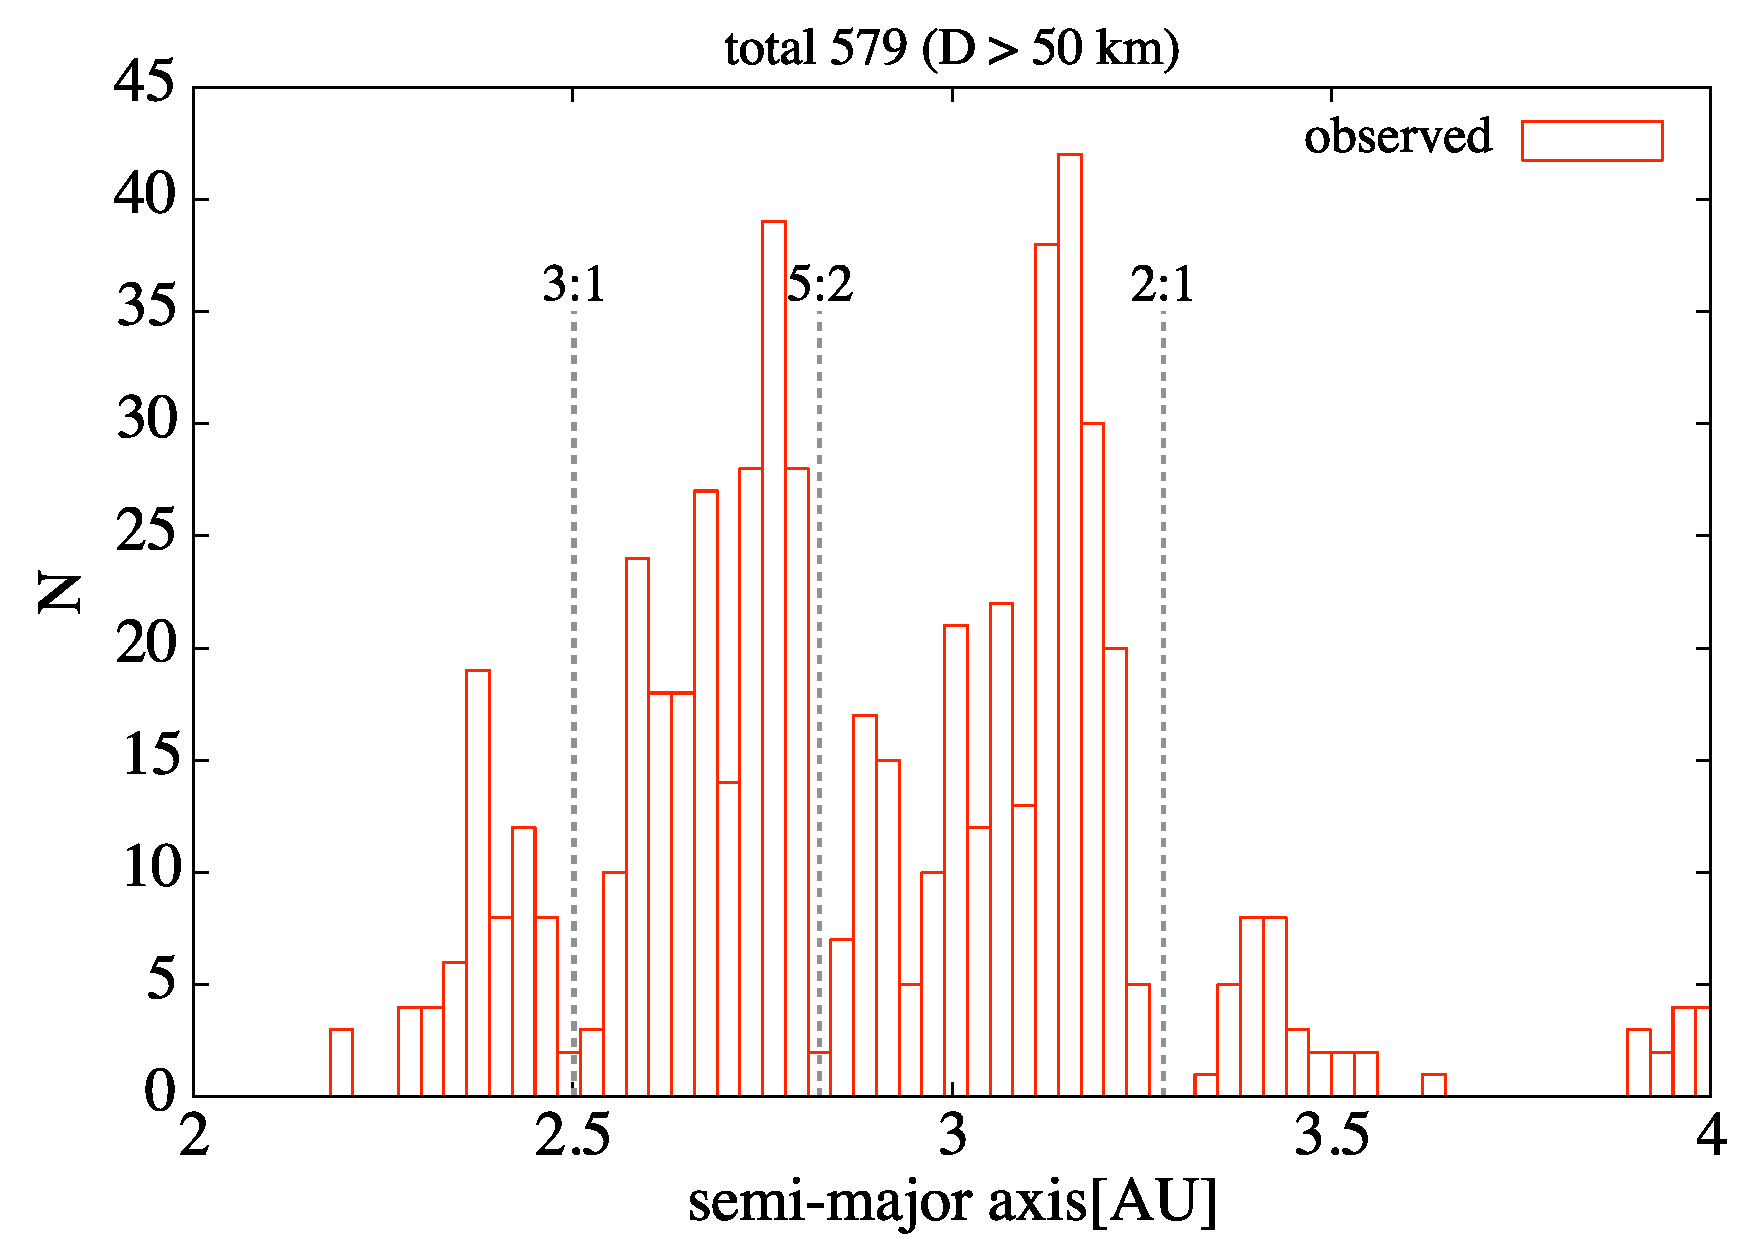
\includegraphics[width=8cm]{./image/mainbelt_histogram.pdf}
\end{minipage} &
%調整
\begin{minipage}[t]{0.1\hsize}
\end{minipage} &
%右
\begin{minipage}[t]{0.45\hsize}
\centering
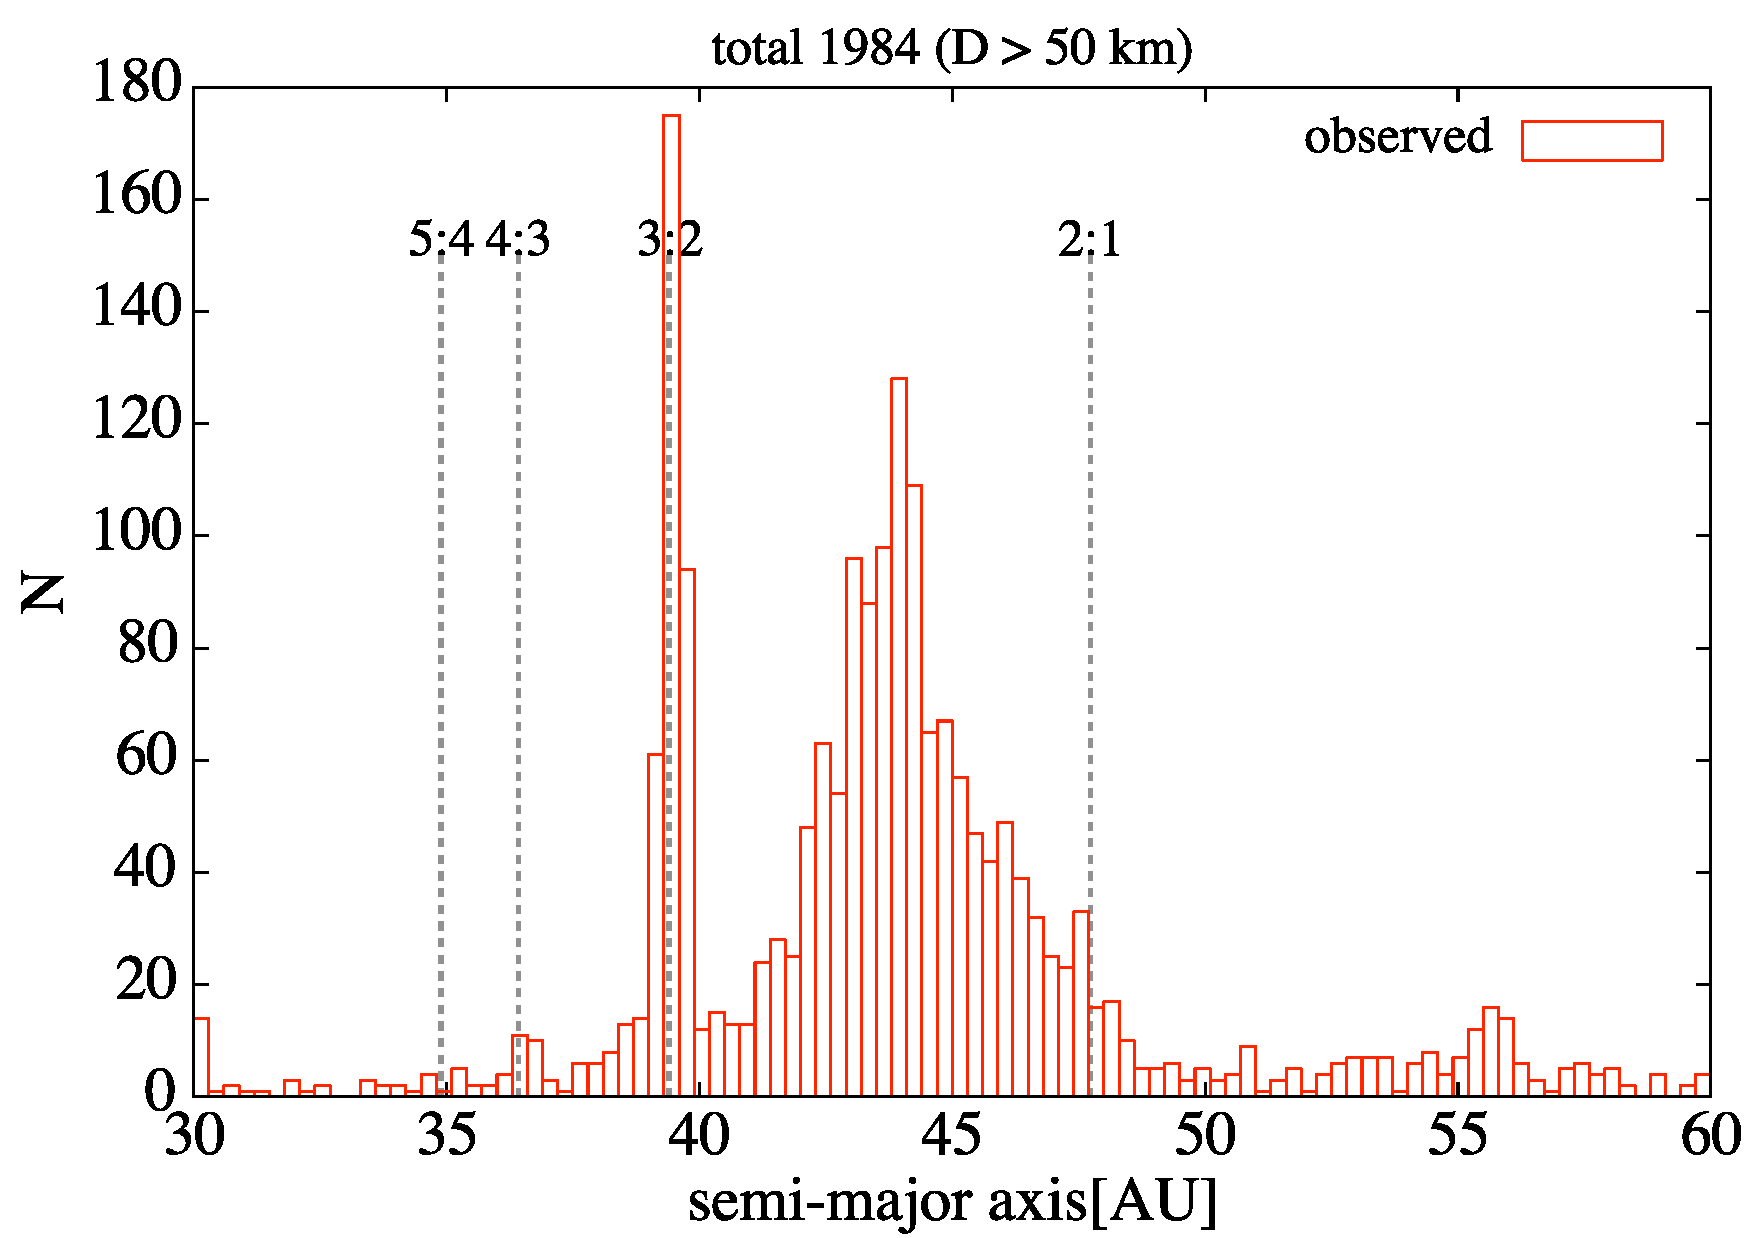
\includegraphics[width=8cm]{./image/kuiperbelt_histogram.pdf}
\end{minipage}\\
%
\end{tabular}
\caption{小惑星帯領域(左)とカイパーベルト領域(右)の小天体の軌道長半径に対する個数分布.各ビンの幅は,小惑星帯:0.03AU,カイパーベルト:0.3AUとしている.\label{fig:obs_histogram}}
\end{figure}

(個数分布の数値計算結果は小惑星帯:図\ref{fig:asteroid_histogram_5Myr} ,カイパーベルト:図\ref{fig:kuiper_histogram_20Myr} で説明している.)
\\

続いて,離心率の分布をみると,小惑星帯は0から0.3まで均等に分布している(図\ref{fig:obs_ecc}左参照).

一方カイパーベルトでは,3:2の尽数関係の位置で0.1から0.3までに集中しており,また3:2と2:1の尽数関係の間の領域では0から0.2までに集中している.また曲線は,近日点距離が30AU(海王星の軌道長半径とほぼ等しい)と一致するときの,軌道長半径と離心率の関係を表しており,大多数の小天体が海王星と軌道交差しない領域にいる中で,3:2の尽数関係の位置には軌道交差しているものが比較的多く存在する(図 \ref{fig:obs_ecc} 右参照).

\begin{figure}[H]
\begin{tabular}{ccc}
%左
\begin{minipage}[t]{0.45\hsize}
\centering
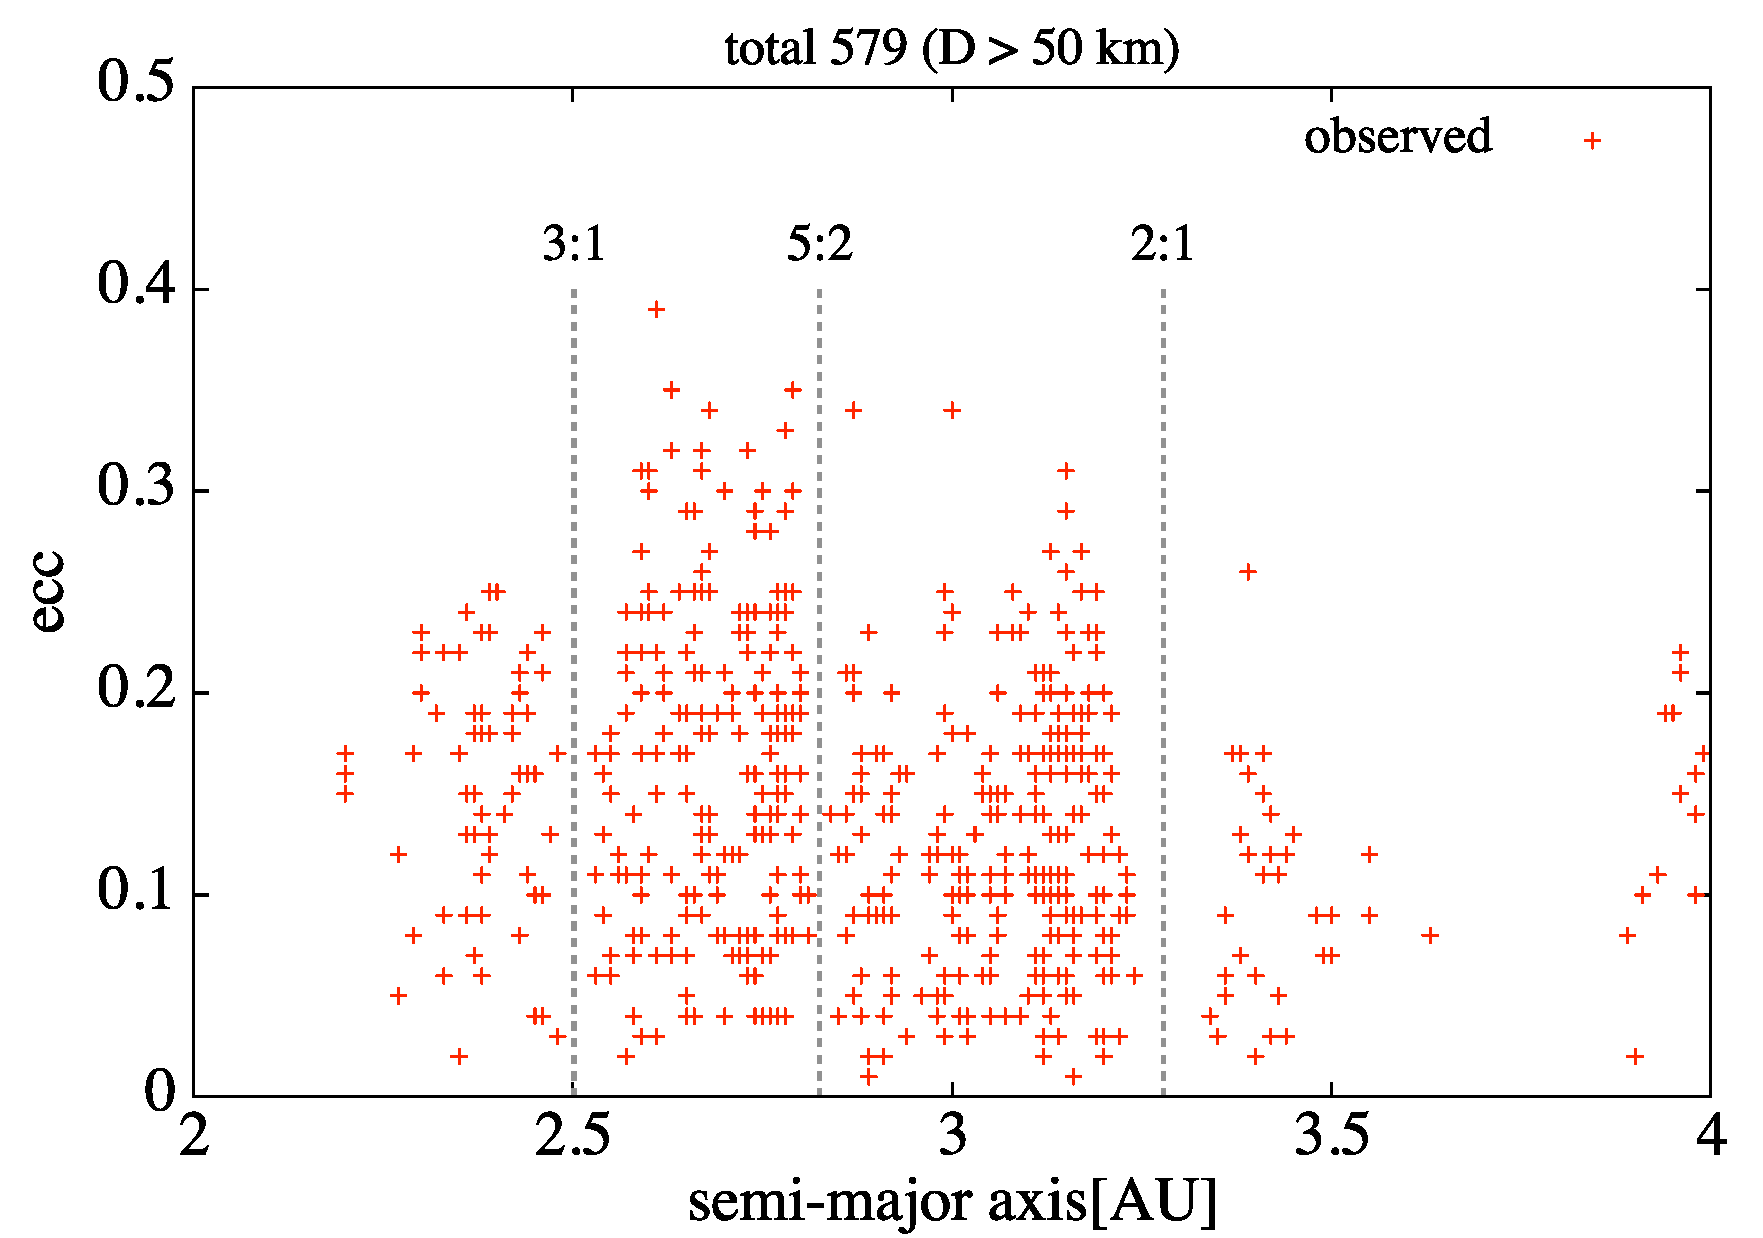
\includegraphics[width=8cm]{./image/mainbelt_ecc.pdf}
\end{minipage} &
%調整
\begin{minipage}[t]{0.1\hsize}
\end{minipage} &
%右
\begin{minipage}[t]{0.45\hsize}
\centering
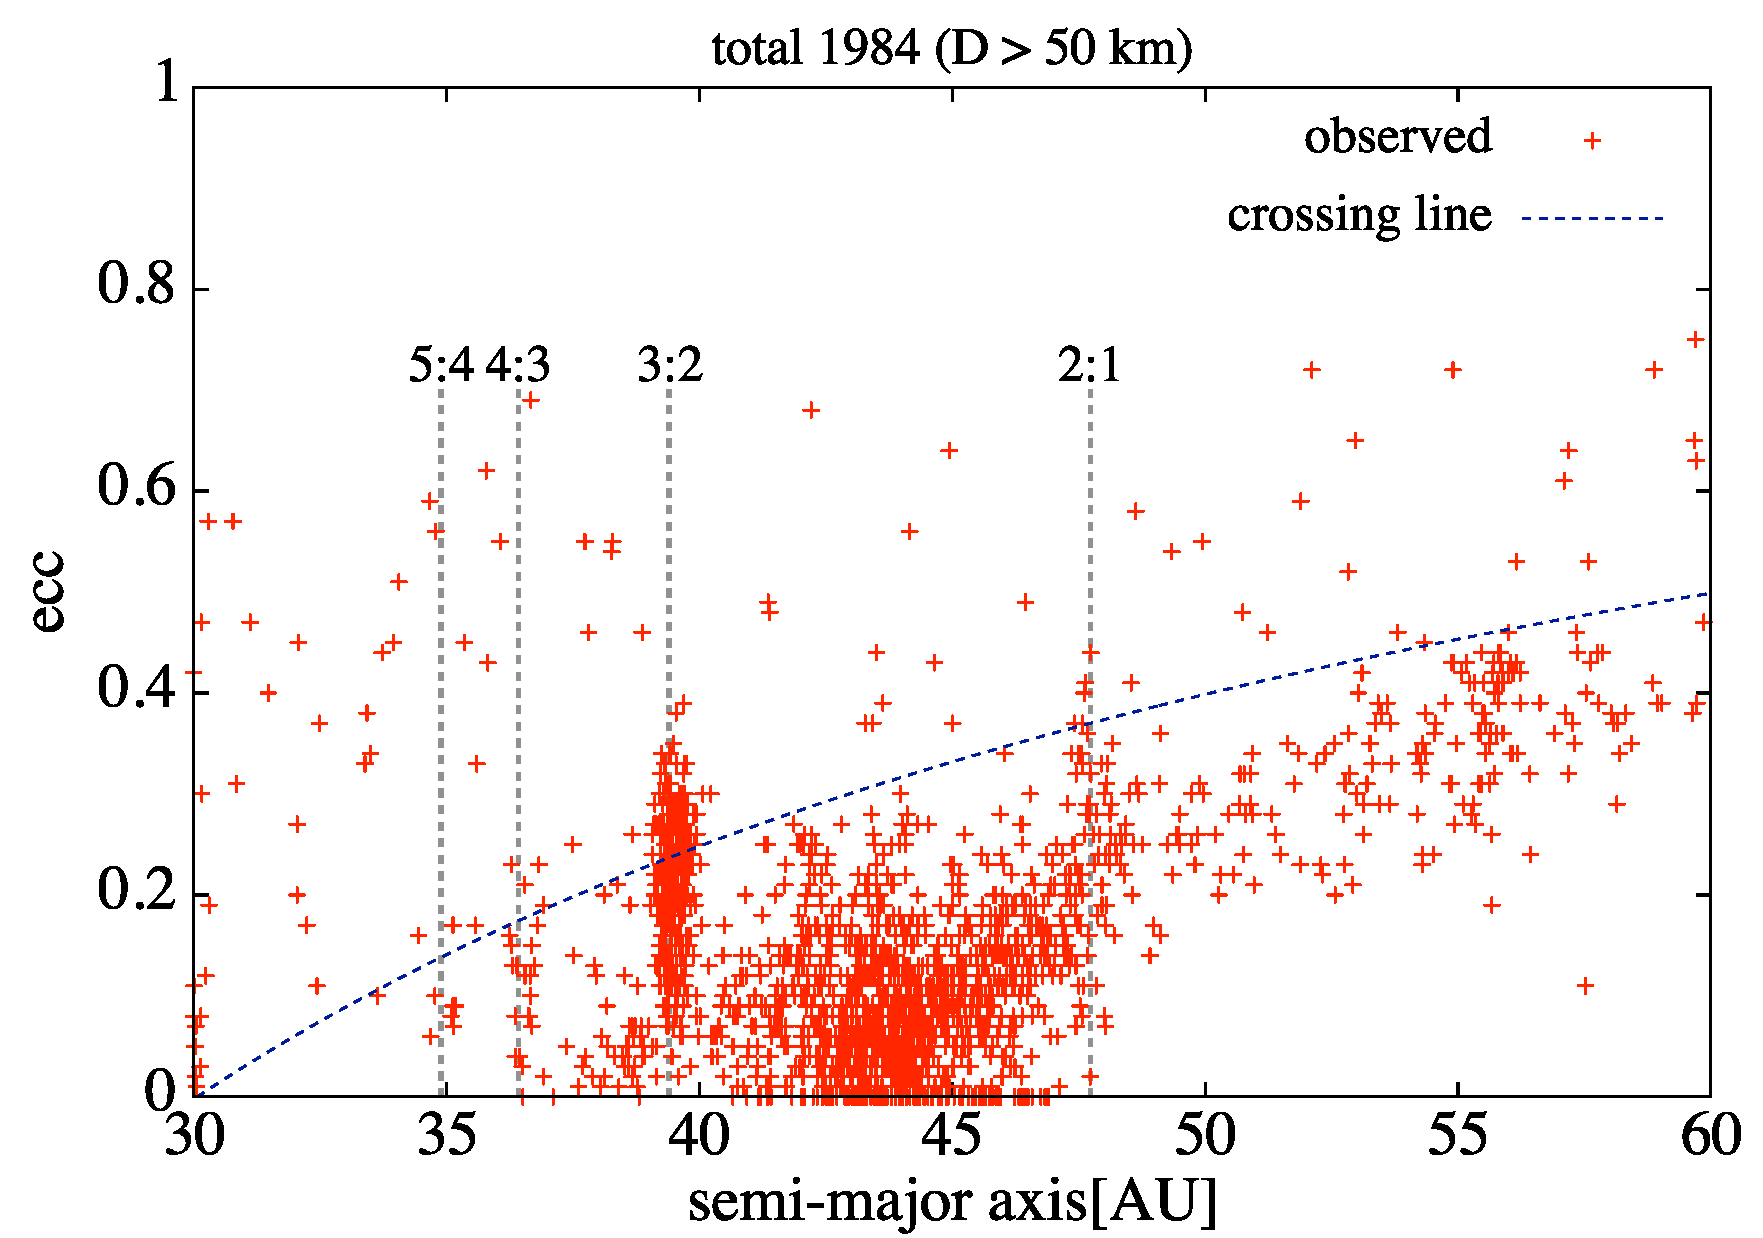
\includegraphics[width=8cm]{./image/kuiperbelt_ecc.pdf}
\end{minipage}\\
%
\end{tabular}
\caption{小惑星帯領域(左)とカイパーベルト領域(右)の小天体の離心率.また近日点距離が $30 {\rm AU}$ と一致するときの,軌道長半径と離心率の関係を曲線で表している.\label{fig:obs_ecc}}
\end{figure}

(離心率の数値計算結果は小惑星帯:図\ref{fig:asteroid_ecc_inc_5Myr}左,カイパーベルト:図\ref{fig:kuiper_ecc_inc_20Myr}左で説明している.)
\\

最後に,軌道傾斜角の分布をみると,先ほどと同様に,小惑星帯は0から0.3\ radまで均等に分布している(図\ref{fig:obs_inc}左参照).

一方カイパーベルトでは,3:2の尽数関係の位置では0から0.6\ radまで均等に分布しているが,42AUから2:1の尽数関係の位置までの領域では0から0.1\ radに集中している.また,軌道長半径が40AUから42AU,軌道傾斜角が0から0.2\ radの領域で,明らかに小天体の数が少ない(図\ref{fig:obs_inc}右参照).

\begin{figure}[H]
\begin{tabular}{ccc}
%左
\begin{minipage}[t]{0.45\hsize}
\centering
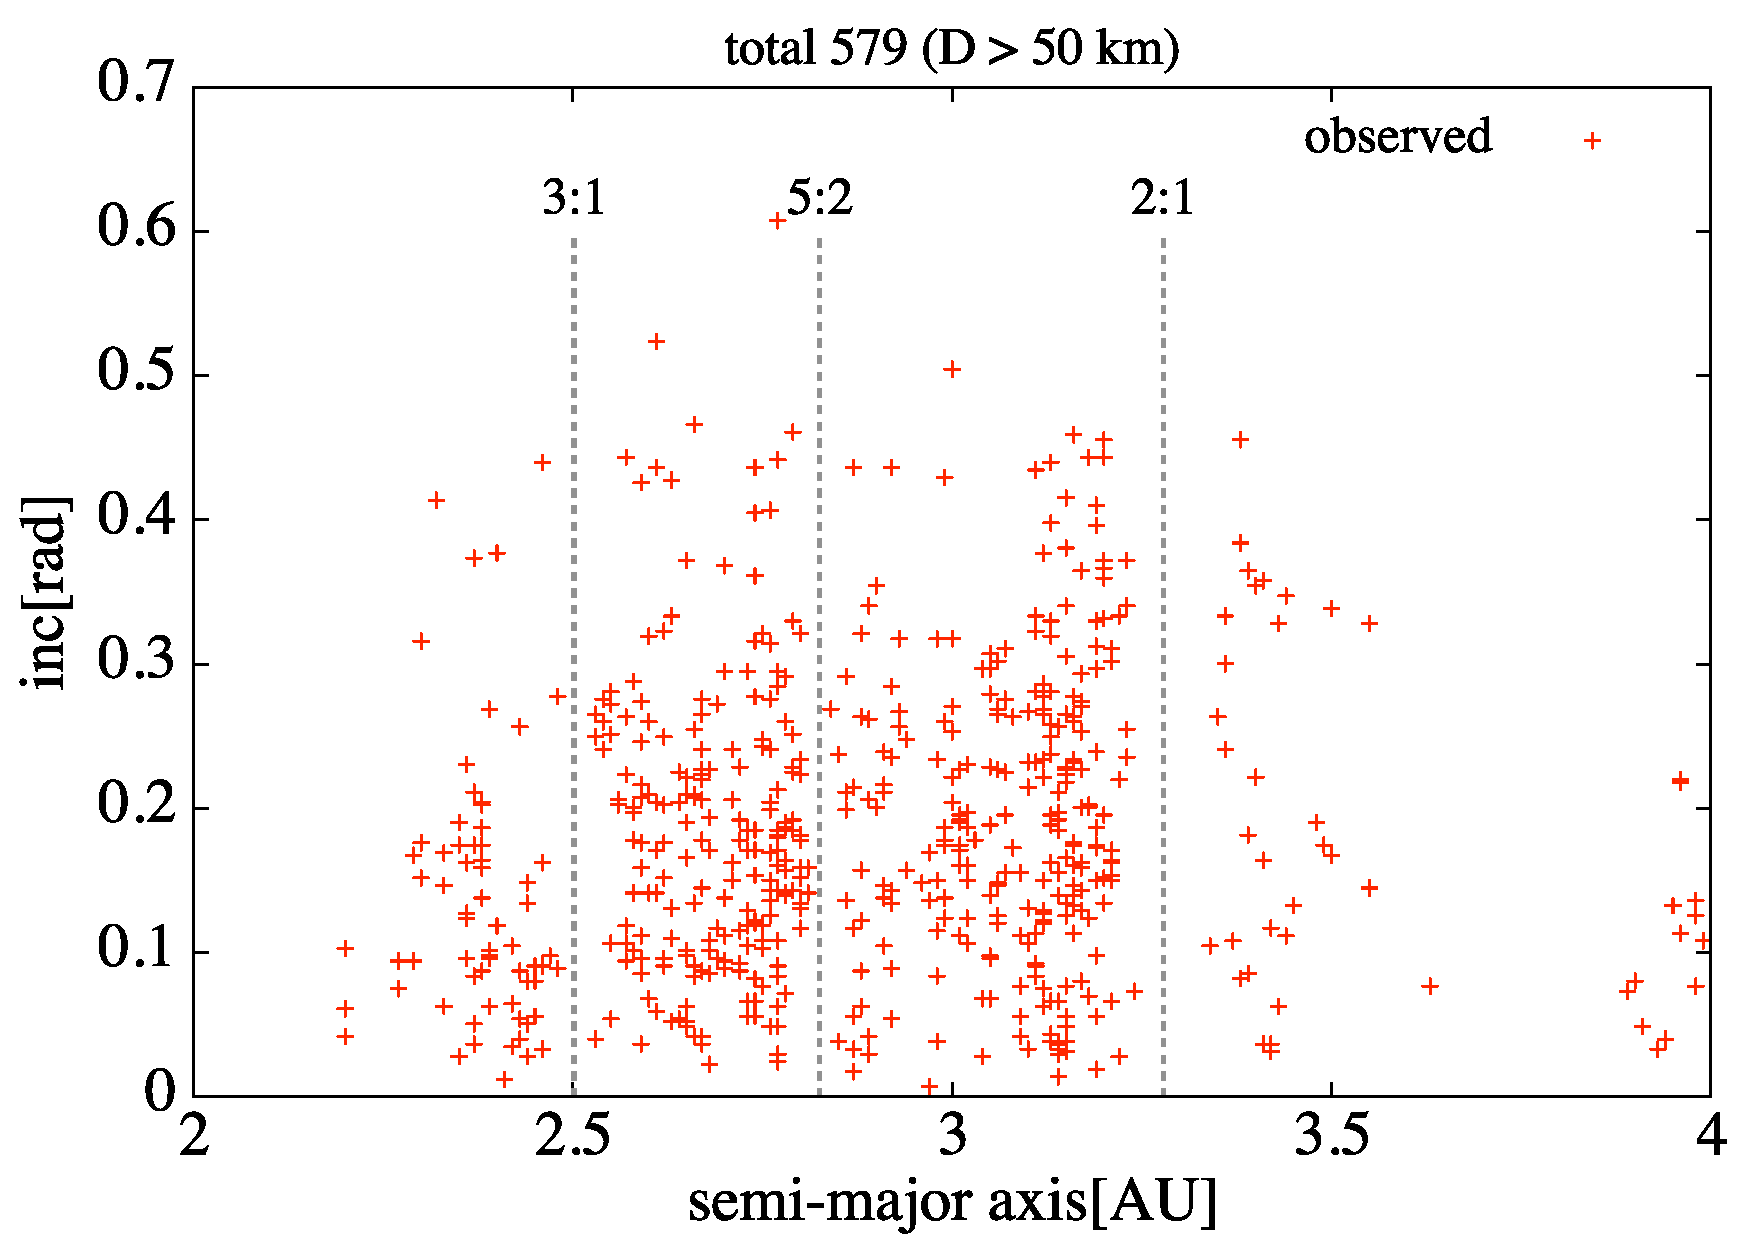
\includegraphics[width=8cm]{./image/mainbelt_inc.pdf}
\end{minipage} &
%調整
\begin{minipage}[t]{0.1\hsize}
\end{minipage} &
%右
\begin{minipage}[t]{0.45\hsize}
\centering
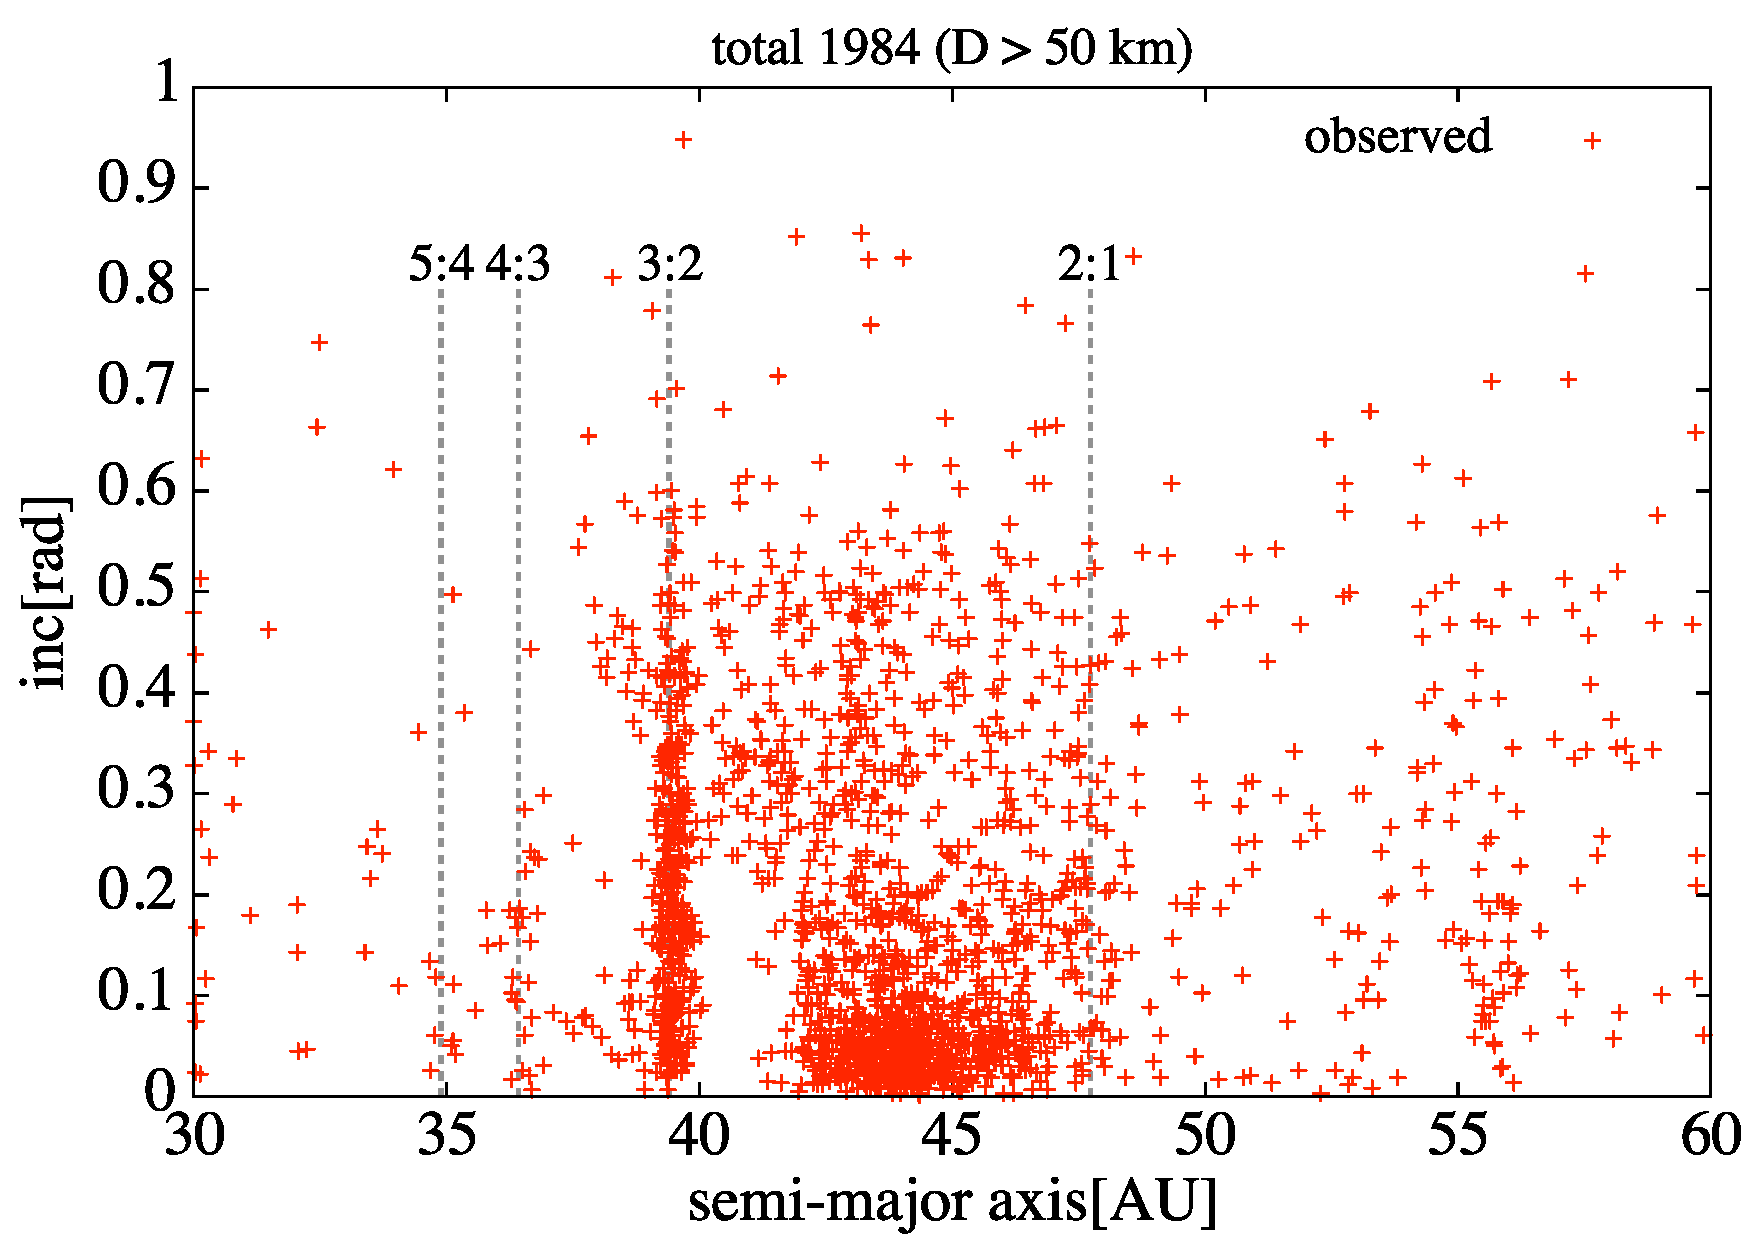
\includegraphics[width=8cm]{./image/kuiperbelt_inc.pdf}
\end{minipage}\\
%
\end{tabular}
\caption{小惑星帯領域(左)とカイパーベルト領域(右)の小天体の軌道傾斜角.\label{fig:obs_inc}}
\end{figure}

(軌道傾斜角の数値計算結果は小惑星帯:図\ref{fig:asteroid_ecc_inc_5Myr}右,カイパーベルト:図\ref{fig:kuiper_ecc_inc_20Myr}右で説明している.)
\\

上で述べたような小天体の軌道の特徴を説明するために,巨大惑星(木星,土星,天王星,海王星)が現在の軌道長半径とは異なる場所で生まれ,時間をかけて移動し,現在の軌道長半径になったとするモデルが提唱され,惑星移動に関する研究が行われてきた.

Malhotraは,カイパーベルトのうち海王星と3:2の尽数関係となる軌道長半径の小天体について,惑星移動を考えたときの離心率と軌道傾斜角の変化について詳しく数値計算をした\cite{Malhotra}.彼が用いた惑星移動モデルは,木星を内側へ0.2AU,土星を外側へ0.8AU,天王星を外側へ3.0AU,海王星を外側へ7.0AU移動させるものである.このモデルの移動距離のうち天王星と海王星は,Fernandezらによる天王星と海王星の2つの惑星と微惑星との角運動量交換を考えたときの数値計算\cite{Fernandez}の範囲内にある.さらに,海王星と3:2の尽数関係となる軌道長半径で小天体の離心率を0.3まで上げるには,海王星の移動距離は最低でも5AU必要であると結論づけている.

Mintonらは,Malhotraと同じ惑星移動モデルを使い,小惑星帯の小天体について詳しく数値計算をした\cite{Minton}.彼らは木星と尽数関係となる軌道長半径でギャップが形成されることを確かめ,また内側にいくほど個数が減っているように見えることの原因として,後に紹介する土星の「永年共鳴」が通過することを挙げた.この土星の永年共鳴が小惑星帯を通過したと考えると,土星の移動距離に強い制約をつけることができるだろうと結論づけている.

すなわち,小惑星帯やカイパーベルトには太陽系の惑星移動の痕跡が残されており,小天体の特徴的な分布がどのように作られたのかについて理解することは,太陽系の歴史を探ることにつながると考えられる.


\chapter{天体力学の基礎}
\thispagestyle{fancy}
この章は本研究に必要な天体力学の基礎を学ぶために,Solar System Dynamics\cite{SSD}の部分訳を載せている.

\section{2体問題 \label{sec:2body}}
2体問題とは,万有引力の法則で記述される2つの質点の相互作用による運動を考える問題である.2体問題は太陽系力学の中で最も単純で,かつ解析的に解くことができる.また,太陽系には様々な質量の物体があるが,2体問題に近似して考えることができる場面が多く,通常3体目の天体との相互作用は2体の系に対する摂動として扱う.
\subsection{運動方程式 \label{sec:EoM}}
2体問題の例として,質量がそれぞれ $m_1, m_2$ の2つの質点を考える.各点の位置ベクトルは ${\bm r}_1, {\bm r}_2$ である.また,$m_1$ を基準とした $m_2$ の相対ベクトルは ${\bm r} = {\bm r}_2 - {\bm r}_1$ と書ける (図\ref{fig:2body}).2つの質点の運動方程式は以下のように書ける.
\begin{equation}
{\bm F}_1 = + G \frac{m_1 m_2}{r^3} {\bm r} = m_1 \ddot{{\bm r}}_1 \quad {\rm and} \quad {\bm F}_2 = - G \frac{m_1 m_2}{r^3} {\bm r} = m_2 \ddot{{\bm r}}_2. \label{eq:F}
\end{equation}
$G = 6.67260 \times 10^{-11} {\rm N m^2 kg^{-2}}$ は重力定数.これらから,
\begin{equation}
m_1 \ddot{{\bm r}}_1 + m_2 \ddot{{\bm r}}_2 = 0. \label{eq:mr}
\end{equation}
が求まる.

\begin{figure}[H]
\centering
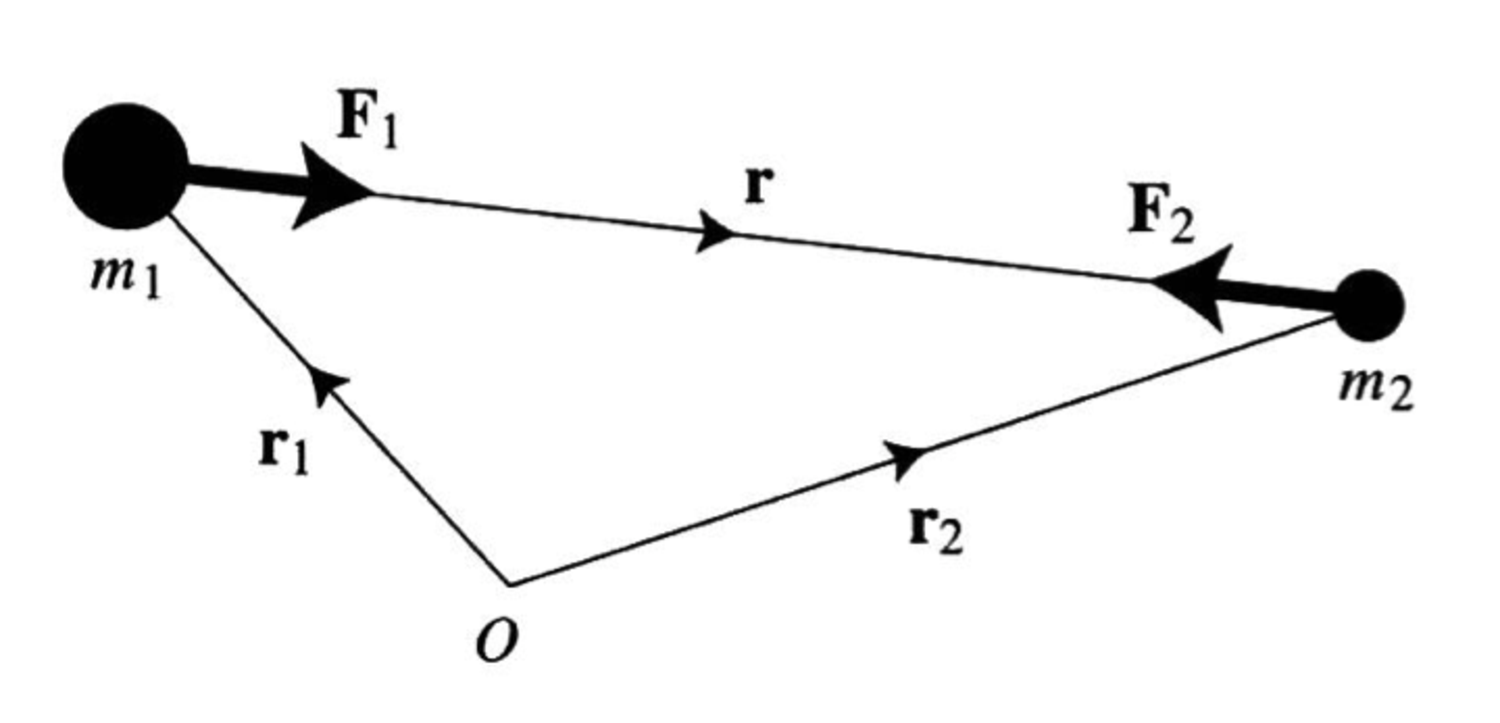
\includegraphics[width=10cm]{./image/sec2_1.pdf}
\caption{位置ベクトル ${\bm r}_1, {\bm r}_2$ にある2つの質点 $m_1, m_2$ に働く力のベクトル図.(Solar System Dynamics\cite{SSD} より引用)\label{fig:2body}}
\end{figure}

式(\ref{eq:mr})を両辺2階積分する.
\begin{equation}
m_1 \dot{{\bm r}}_1 + m_2 \dot{{\bm r}}_2 = {\bm a} \quad {\rm and} \quad m_1 {\bm r}_1 + m_2 {\bm r}_2 = {\bm a} t + {\bm b}.
\end{equation}
${\bm a}, {\bm b}$ は定数ベクトル.${\bm R} = (m_1 {\bm r}_1 + m_2 {\bm r}_2)/(m_1 + m_2)$ を使って重心の位置ベクトルを表現する.
\begin{equation}
\dot{{\bm R}} = \frac{{\bm a}}{m_1 + m_2} \quad {\rm and} \quad {\bm R} = \frac{{\bm a} t + {\bm b}}{m_1 + m_2}.
\end{equation}
この式から,2体が互いの重力のみで運動している場合,その重心の運動は静止しているか,等速直線運動を行っているかのどちらかということになる.ここで,相対ベクトル ${\bm r}$ を使って運動方程式を書き直す.$\ddot{{\bm r}} = \ddot{{\bm r}}_2 - \ddot{{\bm r}}_1$ とすると式(\ref{eq:F})は,
\begin{equation}
\frac{d^2 {\bm r}}{dt^2} + \mu \frac{{\bm r}}{r^3} = 0. \label{eq:raletive}
\end{equation}
($\mu = G (m_1 + M_2)$) となり,相対運動の方程式となる.この方程式を解き $m_2$ の $m_1$ に対する相対軌道を得るためには,相対運動におけるいくつかの定数を求める必要がある. ここではまずそれらの運動の定数の一つである角運動量ベクトルについて述べる.

式(\ref{eq:raletive})の両辺と ${\bm r}$ の外積をとると,${\bm r} \times \ddot{{\bm r}} = 0$.さらに両辺積分すると,
\begin{equation}
{\bm r} \times \dot{{\bm r}} = {\bm h} \label{eq:angmom}
\end{equation}
${\bm h}$ は角運動量ベクトルであり,${\bm r}, \dot{{\bm r}}$ に垂直である定数ベクトルである.つまり,$m_2$ の相対運動は,${\bm r}, \dot{{\bm r}}$ に垂直な平面内に限定されることがわかる.この平面を軌道平面という.$m_2 \ll m_1$ とすれば $h = |{\bm h}|$ は単位質量あたりの $m_2$ の角運動量として近似できる.

ここで,${\bm r}$ を極座標で表現してみよう.座標原点は $m_1$ とし,$\theta = 0$ となる基準線は任意の位置でとることとする.また $m_1, m_2$ の重心は慣性系を運動しているが,$\theta = 0$ の基準線の方向は一定とする.動径方向の単位ベクトルを $\hat{{\bm r}}$,角度方向の単位ベクトルを $\hat{{\bm \theta}}$ として,位置,速度,加速度を表現すると以下のようになる.
\begin{equation}
{\bm r} = r \hat{{\bm r}}, \quad \dot{{\bm r}} = \dot{r} \hat{{\bm r}} + r \dot{\theta} \hat{{\bm \theta}}, \quad \ddot{{\bm r}} = (\ddot{r} - r \dot{\theta}^2) \hat{{\bm r}} + \left[ \frac{1}{r} \frac{d}{dt} (r^2 \dot{\theta})\right] \hat{{\bm \theta}}. \label{eq:polar}
\end{equation}

式(\ref{eq:angmom})に上記の ${\bm r}, \dot{{\bm r}}$ を代入すると,${\bm h} = r^2 \dot{\theta} \hat{{\bm z}}$ となる.$\hat{{\bm z}}$ は軌道平面に垂直な単位ベクトルであり,向きは ${\bm r}$ から ${\bm \theta}$ へ右ねじを回したときに進む方向である.これより,
\begin{equation}
h = r^2 \dot{\theta}.
\end{equation}
この式からわかることは以下の通りである.

質点 $m_2$ が微小時間 $\delta t$ の間だけ運動したとする.$t = 0$ のとき $m_2$ の座標が ($r, \theta$) とすれば,$t = \delta t$ の座標は ($r + \delta r, \theta + \delta \theta$) である.その間に動径ベクトルが横切る領域の面積は,
\begin{equation}
\delta A \approx \frac{1}{2} r (r + \delta r) \sin (\delta \theta) \approx \frac{1}{2} r^2 \delta \theta. 
\end{equation}
両辺を $\delta t$ で割り,$\delta t \rightarrow 0$ の極限をとると,
\begin{equation}
\frac{dA}{dt} = \frac{1}{2} r^2 \frac{d \theta}{dt} = \frac{1}{2} r^2 \dot{\theta} = \frac{1}{2} h. \label{eq:kepler2}
\end{equation}
$h$ は定数であるので,動径が一定時間に横切る軌道面の面積は常に一定であることがわかる.つまり 式(\ref{eq:kepler2})は Kepler の第2法則 と等価である.しかし,このことは万有引力に対してのみ成り立つ訳ではなく,2物体の間に引力が働いていれば成り立つ.

\subsection{軌道と速度 \label{sec:position&velocity}}
式(\ref{eq:polar})の $\ddot{{\bm r}}$ を式(\ref{eq:raletive})に代入することで,相対運動のスカラー方程式を求めることができる.$r$ 成分を比べると,
\begin{equation}
\ddot{r} - r \dot{\theta}^2 = - \frac{\mu}{r^2}. \label{eq:scalar}
\end{equation}
$\theta$ の関数としての $r$ の解を求めるため,$u = 1/r$ として代入し,定数 $h = r^2 \dot{\theta}$ を使って時間 $t$を消去する必要がある.$r$ を時間微分すると,
\begin{equation}
\dot{r} = - \frac{1}{u^2} \frac{du}{d \theta} \dot{\theta} \quad {\rm and} \quad \ddot{r} = - h \frac{d^2 u}{d \theta^2} \dot{\theta} = - h^2 u^2 \frac{d^2 u}{d \theta^2}. 
\end{equation}
したがって式(\ref{eq:scalar})を書き換えると,
\begin{equation}
\frac{d^2 u}{d \theta^2} + u = \frac{\mu}{h^2}.
\end{equation}
この2階線形微分方程式の一般解は,
\begin{equation}
u =\frac{\mu}{h^2} \left[ 1+ e \cos (\theta - \varpi) \right].
\end{equation}
ここで振幅 $e$,位相 $\varpi$ は積分定数.よって $r$ は,
\begin{equation}
r =\frac{p}{1+ e \cos (\theta - \varpi)}.
\end{equation}
$p = h^2 / \mu$ は半直弦 ($\theta - \varpi = \pi / 2$ における $r$ の大きさ),$e$ は離心率と呼ばれる.この式は円錐曲線と呼ばれる.

円錐曲線から得られる曲線は $e$ によって区別され,4種類ある.
\begin{equation}
\begin{split}
円 &: \quad e = 0, \quad p = a; \\
楕円 &: \quad 0 < e < 1, \quad p = a(1-e^2); \\
放物線 &: \quad e = 1, \quad p = 2q; \\
双曲線 &: \quad e > 1, \quad p = a(e^2-1). 
\end{split}
\end{equation}
$a$ は軌道長半径.放物線の場合は $p$ を $q$ (放物線の近点距離) で定義する.

この2体問題の解から,太陽系の惑星の軌道は楕円の形をしており,閉じた軌道を描くと
考えられる.したがってKeplerの第1法則は逆2乗則の結果ととらえることができる.

\begin{figure}[H]
\centering
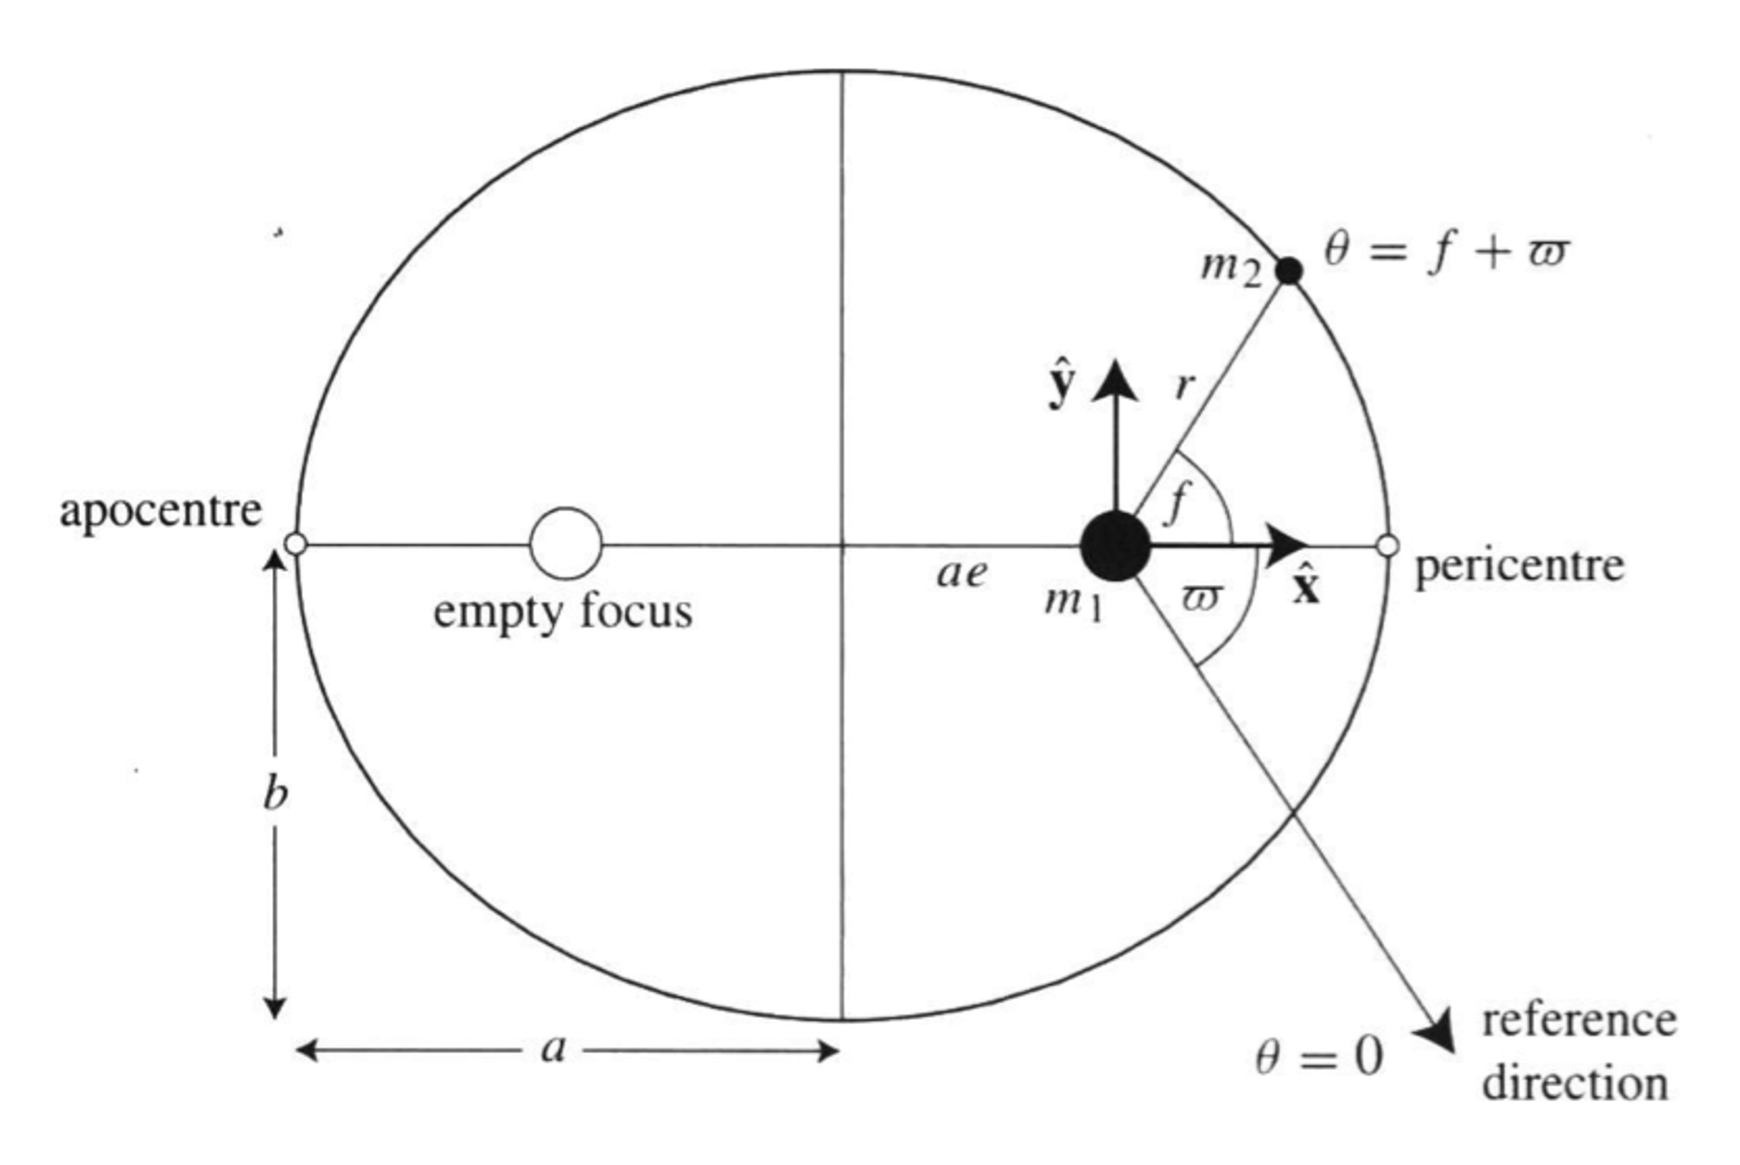
\includegraphics[width=10cm]{./image/sec2_5.pdf}
\caption{軌道長半径 $a$,軌道短半径 $b$,離心率 $e$,近日点経度 $\varpi$ の楕円の図.(Solar System Dynamics\cite{SSD} より引用)\label{fig:ellipse}}
\end{figure}

彗星はその多くが $e \approx 1$ の値を持つのに対して,冥王星 ($e = 0.25$),水星 ($e = 0.21$),そして海王星の衛星 Nereid ($e = 0.75$) という例外があるが,太陽系の主な天体のほとんどは $e \ll 1$ である.したがって,以下の議論では楕円運動に焦点を当てる.

楕円運動では $a, e$ には以下のような関係がある.
\begin{equation}
b^2 = a^2 (1 - e^2).
\end{equation}
ここで $b$ は軌道短半径である (図\ref{fig:ellipse}).また $r$ は,
\begin{equation}
r =\frac{a (1 - e^2)}{1+ e \cos (\theta - \varpi)}.
\end{equation}
$\theta$ は黄経 (黄道座標の経度にあたり,春分点を0度としている) と呼ばれる.天体力学では,慣性系において固定された基準線からの角度を測るときに,慣習的に黄経を用いる.$\theta = \varpi, \theta = \varpi + \pi$ のときに,それぞれ $r$ の最小値 $r_{\rm p} = a (1 - e)$,最大値 $r_{\rm a} = a (1 + e)$ をとる.これらの点はそれぞれ近点,遠点と呼ばれる.楕円の中心からどちらかの焦点までの距離は $a e$ で与えられる.$\varpi$ ("curly pi" と発音) は近日点経度と呼ばれ,近点の黄経である.2体問題では $\varpi$ は定数であるが,他の摂動が入る場合は時間とともに変化する.大抵は黄経よりも $\varpi$ から測った角度の方がより扱いやすく,真近点離角 $f = \theta - \varpi$ を導入する.$f, \theta$ は $2 \pi$ の周期を持つ.よって $r$ は,
\begin{equation}
r = \frac{a (1 - e^2)}{1+ e \cos f}. \label{eq:rf}
\end{equation}
ここで,$m_1$ を中心として近点方向に $x$ 軸をとる直交座標を考えると,位置ベクトルの成分は,
\begin{equation}
x = r \cos f \quad {\rm and} \quad y = r \sin f. \label{eq:xy}
\end{equation}

ある軌道周期 $T$ で楕円上を一周するときに位置ベクトルが横切る面積は単純に $A = \pi a b$ である.(\ref{eq:kepler2}) 式よりこの面積は $h T / 2$ と等しい.ゆえに $h^2 = \mu p = \mu a (1 - e^2)$ より,
\begin{equation}
T^2 = \frac{4 \pi^2}{\mu} a^3. \label{eq:kepler3}
\end{equation}
これは Kepler の第3法則と等価である.この式から軌道周期 $T$ は離心率 $e$ に依存せず,軌道長半径 $a$ のみに依存することがわかる.

$\theta$ は 1周期につき $2 \pi$ だけ周期的に変化するため,平均運動 $n$ を次のように定義する.
\begin{equation}
n = \frac{2 \pi}{T}. \label{eq:n}
\end{equation}
さらに,式(\ref{eq:kepler3})より,
\begin{equation}
\mu = n^2 a^3 \quad {\rm and} \quad h = n a^2 \sqrt{1 - e^2} = \sqrt{\mu a (1 - e^2)}. \label{eq:mu}
\end{equation}
平均運動の値は2体問題では定数であるが,実際の角速度 $\dot{f}$ は経度の関数である.

運動に関するもう一つの定数を導出するため,$\dot{{\bm r}}$ と 式(\ref{eq:raletive})の内積をとり,式(\ref{eq:polar})の ${\bm r}, \ddot{{\bm r}}$ の値を代入すると,
\begin{equation}
{\bm r} \cdot \ddot{{\bm r}} + \mu \frac{\dot{{\bm r}}}{r^2} = 0.
\end{equation}
これを両辺 $t$ で積分すると,
\begin{equation}
\frac{1}{2} v^2 - \frac{\mu}{r} = C. \label{eq:energyC}
\end{equation}
ここで $v^2 = \dot{{\bm r}} \cdot \dot{{\bm r}}$ は速度の2乗,$C$ は積分定数である.式(\ref{eq:energyC})はエネルギー積分とも呼ばれ,単位質量あたりの天体のエネルギーが保存することを示している.ここまでの結果より,2体問題には4つの定数が保存する : エネルギー積分 $C$ と角運動量 ${\bm h}$ の3成分である.\ref{sec:elements} 節で導出するが,これらは軌道要素や離心率ベクトルのような別の量で表現することもできる.

$v^2$ の別の表式を見つけ, $C$ の別の表式を導出する.$\varpi$ は固定されているので,$\dot{\theta} = d (f + \varpi) / dt = \dot{f}$ であり,式(\ref{eq:polar})の ${\bm r}$ の定義を用いると,
\begin{equation}
v^2 = \dot{{\bm r}} \cdot \dot{{\bm r}} = \dot{r}^2 + r^2 \dot{f}^2. \label{eq:v2}
\end{equation}
式(\ref{eq:rf})を微分すると,
\begin{equation}
\dot{r} = \frac{r \dot{f} e \sin f}{1+ e \cos f}.
\end{equation}
$r^2 \dot{f} = h = n a^2 \sqrt{1 - e^2}$ を使うと,
\begin{eqnarray}
\dot{r} & = & \frac{n a}{\sqrt{1 - e^2}} e \sin f, \label{eq:rdot} \\
r \dot{f} & = & \frac{n a}{\sqrt{1 - e^2}} (1+ e \cos f). \label{eq:rfdot}
\end{eqnarray}
この2つの式から式(\ref{eq:v2})を書き換えると,
\begin{equation}
v^2 = \frac{n a^2}{1 - e^2} (1 + 2 e \cos f + e^2) = \frac{n a^2}{1 - e^2} \left( \frac{2 a (1 - e^2)}{r} - (1 - e^2) \right).
\end{equation}
したがって,
\begin{equation}
v^2 = \mu \left( \frac{2}{r} - \frac{1}{a} \right). \label{eq:v2new}
\end{equation}
この式から,天体の速度は近点 ($f = 0$) で最大値,遠点 ($f = \pi$) で最小値をとる.それぞれの値は,
\begin{equation}
v_{\rm p} = n a \sqrt{\frac{1 + e}{1 - e}} \quad {\rm and} \quad v_{\rm a} = n a \sqrt{\frac{1 - e}{1 + e}}.
\end{equation}

また,式(\ref{eq:xy})をそれぞれ時間微分し,式(\ref{eq:rdot}),  式(\ref{eq:rfdot})を代入して,速度の $x, y$ 成分を求めると,
\begin{equation}
\dot{x} = - \frac{n a}{\sqrt{1 - e^2}} \sin f \quad {\rm and} \quad  \dot{y} = + \frac{n a}{\sqrt{1 - e^2}} (e^2 + \cos f). \label{eq:xdotydot}
\end{equation}

式(\ref{eq:v2new})と式(\ref{eq:energyC})を比較すると,エネルギー積分 $C$ は以下の形で表される.
\begin{equation}
C = - \frac{\mu}{2 a}. \label{eq:C}
\end{equation}
したがって,楕円軌道のエネルギーは軌道長半径のみの関数であり,離心率には依存しない.放物線軌道と双曲線軌道のエネルギーも同様に示すことができる.
\begin{equation}
C_{{\rm para}} = 0, \quad {\rm and} \quad C_{{\rm hyper}} = \frac{\mu}{2 a}.
\end{equation}

\subsection{平均近点離角と離心近点離角}
前節において,軌道長半径と離心率がわかっている場合に,真近点離角 $f$ が与えられれば,軌道の距離と速度を計算できることを示した.しかし,通常は任意の時間での天体の位置を計算したいと考えるのが普通である.$f$ と $r$ は $t$ の関数であるが,前節では依存性を示していない.

$2 \pi$ 周期かつ時間に関して線形な関数である角度を導入する.この角度は,後にさまざまな量の時間平均を計算するときに特に有益となる.式(\ref{eq:n})の平均運動 $n$ の定義を用いて,平均近点離角 $M$ を定義する.
\begin{equation}
M = n (t - \tau). \label{eq:M}
\end{equation}
ここで,$\tau$ は近点通過時刻.$M$ は角度の次元であり,平均運動と等しい一定の割合で線形的に増加するが,幾何学的に意味のある値ではない.しかし,$M$ の定義と式(\ref{eq:rf})から,$t = \tau$ (近点を通過) や $t = \tau + T / 2$ (遠点を通過) のとき,それぞれ $M = f =0, M = f = \pi$ となることは明らかである.$t$ が周期の整数倍のときも同様の関係を持つ.

$M$ は幾何学的に意味のある値ではないが,ある角度と関係がある.半径 $a$ の円を,軌道長半径 $a$,離心率 $e$ の楕円に外接させ (図\ref{fig:Ef}(a)),その楕円のある点から長軸に垂直な直線を引き,外接円に交差させる. すると,$f = 0$ の基準線 (長軸) と,楕円の中心からその外接円上の交点までを結ぶ直線とのなす角で定義される,離心近点離角 $E$ という角度を決めることができる (図\ref{fig:Ef}(b)).したがって,$E = 0$ は $f = 0$ と一致し,$E = \pi$ は $f = \pi$ と一致する.

\begin{figure}[H]
\centering
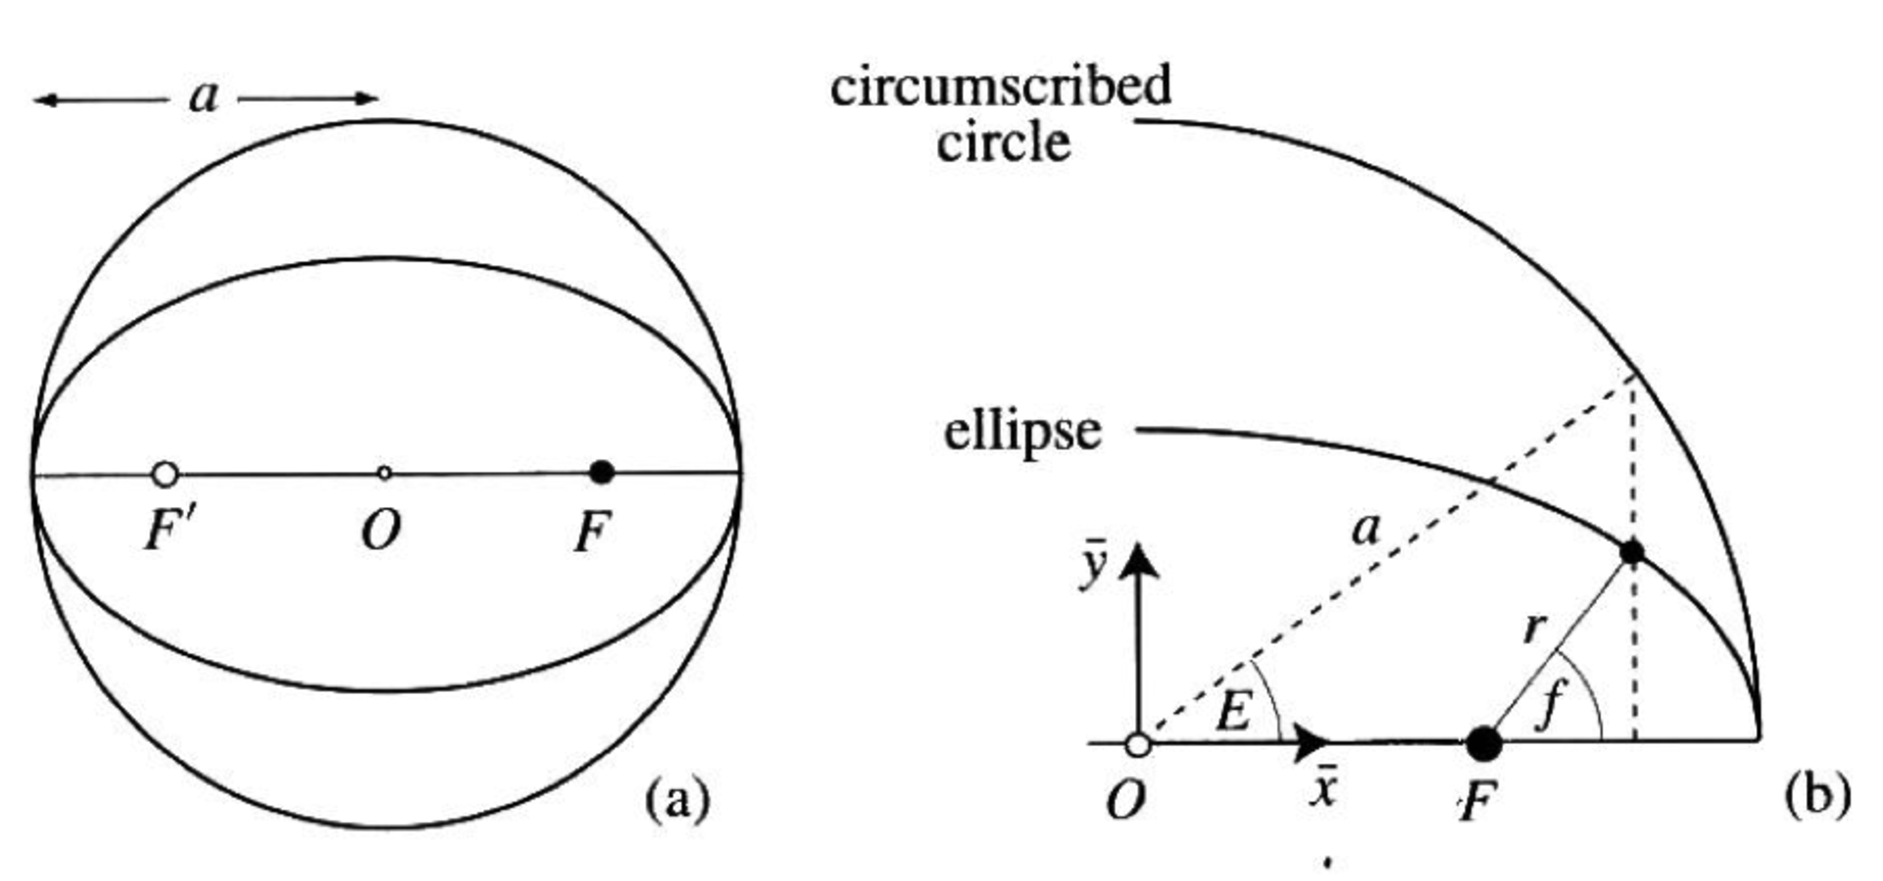
\includegraphics[width=10cm]{./image/sec2_7.pdf}
\caption{(a) 軌道長半径 $a$ の楕円と,半径 $a$ の外接円.(b) 真近点離角 $f$ と離心近点離角 $E$ の関係.(Solar System Dynamics\cite{SSD} より引用)\label{fig:Ef}}
\end{figure}

図 \ref{fig:Ef} (b) 中の $\bar{x}, \bar{y}$ のように楕円中心を原点にとる直交座標系での楕円の方程式は,
\begin{equation}
\left( \frac{\bar{x}}{a} \right)^2 + \left( \frac{\bar{y}}{b} \right)^2 = 1.
\end{equation}
$\bar{x} = e \cos E$ から $\bar{y}^2 = b^2 \sin^2 E$ が求まり,$b^2 = a^2 (1 - e^2)$ の関係から $\bar{y} = a \sqrt{1 - e^2} \sin E$ が求まる.したがって外接円への $r$ の水平方向と垂直方向の射影は,$E$ を用いて表すと,
\begin{equation}
x = a (\cos E - e) \quad {\rm and} \quad y = a \sqrt{1 - e^2} \sin E. \label{eq:xEyE}
\end{equation}
これらの2乗和の平方根をとると,
\begin{eqnarray}
r & = & a (1 - e \cos E), \label{eq:rE} \\
\cos f & = & \frac{\cos E - e}{1 - e \cos E}. \label{eq:fE}
\end{eqnarray}
さらに,離心近点離角 $E$ と真近点離角 $f$ の関係のより簡単な表式が導出できる.
\begin{equation}
1 - \cos f = \frac{(1 + e) (1 - \cos E)}{1 - e \cos E}, \quad 1 + \cos f = \frac{(1 - e) (1 + \cos E)}{1 - e \cos E}.
\end{equation}
三角関数の2倍角の公式を使えば,
\begin{equation}
2 \sin^2 \frac{f}{2} = \frac{1 + e}{1 - e \cos E} 2 \sin^2 \frac{E}{2}, \quad 2 \cos^2 \frac{f}{2} = \frac{1 - e}{1 - e \cos E} 2 \cos^2 \frac{E}{2}.
\end{equation}
ゆえに,
\begin{equation}
\tan \frac{f}{2} = \sqrt{\frac{1 + e}{1 - e}} \tan \frac{E}{2}. \label{eq:fEnew}
\end{equation}
したがって,$E$ がわかっているとき,式(\ref{eq:rE})を使えば $r$ を,式(\ref{eq:fE})または式(\ref{eq:fEnew})を使えば $f$ を決定することができる.しかし,任意の時間 $t$ における天体の位置を知るには,$M$ と $E$ の関係を明らかにする必要がある.

$v^2 = \dot{r}^2 + (r \dot{f})^2$ と式(\ref{eq:rfdot}),式(\ref{eq:v2new})を使うと,
\begin{eqnarray}
\dot{r}^2 & = & n^2 a^3 \left( \frac{2}{r} - \frac{1}{a} \right) - \frac{n^2 a^4 (1 - e^2)}{r^2}, \\
\frac{dr}{dt} & = & \frac{na}{r} \sqrt{a^2 e^2 - (r - a)^2}. \label{eq:drdt}
\end{eqnarray}
この式は式(\ref{eq:rE})を用いた以下の置き換えで積分可能となる.
\begin{equation}
r - a = - a e \cos E.
\end{equation}
よって式(\ref{eq:drdt})は,
\begin{equation}
\frac{dE}{dt} = \frac{n}{1 - e \cos E}. \label{eq:dEdt}
\end{equation}
この式は式(\ref{eq:xEyE})をそれぞれ時間微分し,${\bm r} \times \dot{{\bm r}} = h ( = n a^2 \sqrt{1 - e^2} )$ に代入することでも求めることができる.式(\ref{eq:dEdt})は簡単に積分できて,
\begin{equation}
n (t - \tau) = E - e \sin E. \label{eq:tauE}
\end{equation}
$t = \tau$ のとき $E = 0$.したがって式(\ref{eq:M})は,
\begin{equation}
M = E - e \sin E. \label{eq:keplereq}
\end{equation}
この式は Kepler 方程式と呼ばれ,その解は,任意の時間における軌道上の位置を求める際になくてはならないものである.ある時間が与えられたとき,(i) 式(\ref{eq:M})から $M$ を求め,(ii) $E$ について式(\ref{eq:keplereq})を解き,(iii) 式(\ref{eq:xEyE})または式(\ref{eq:fE})と,式(\ref{eq:rf})を使って$r, f$ を決める.

\subsection{軌道要素 \label{sec:elements}}
\ref{sec:EoM}節では,$m_1$ に対する $m_2$ の相対位置ベクトルと速度ベクトルが,常に角運動量ベクトルに垂直な平面上に存在することを示した.$m_2$ の ${\bm r} = (x, y)$ と $\dot{\bm r} = (\dot{x}, \dot{y})$ は3つの定数 $a, e, \varpi$ と変数 $f$ によって固有の値をもつ.ここまでの解析では軌道面上の運動を理解してきた.しかし,太陽系の天体の運動は単一の基準面上で起こるものではなく,ここからは軌道の3次元表現を考えていく (図\ref{fig:elements_SSD}).
 
任意の位置が位置ベクトル ${\bm r} = (x, y, z) = x \hat{\bm x} + y \hat{\bm y} + z \hat{\bm z}$ で表現される3次元直交座標系を考える.3つの軸が右手系をなすように,$x$ 軸は楕円軌道の長軸上の近点の方向,$y$ 軸は 軌道面上の$x$ 軸に垂直な方向,そして $z$ 軸は $x, y$ 軸両方に垂直で $\hat{\bm x} \times \hat{\bm y}$ の方向にとる.

この軌道面から基準面を参照するために,基準面上の基準線の方向を $X$ 軸にとるような別の3次元直交座標系を考える.上と同様に3つの軸が右手系をなすように,$Y$  軸は基準面上の$X$ 軸に垂直な方向,そして $Z$ 軸は $X, Y$ 軸両方に垂直で $\hat{\bm X} \times \hat{\bm Y}$ の方向にとる.この座標系の例として,太陽のまわりを回る惑星の運動の場合,日心座標系 (太陽を中心とし,基準面を地球軌道面 (黄道面),基準線を地球の赤道面と黄道面の交線に沿った方向,すなわち春分の方向にとる座標系) が慣習的に使われる.注意すべきことは,他の天体による摂動を受けるため,特定の基準面を決めてもその基準面は時間変化してしまうことである.

\begin{figure}[H]
\centering
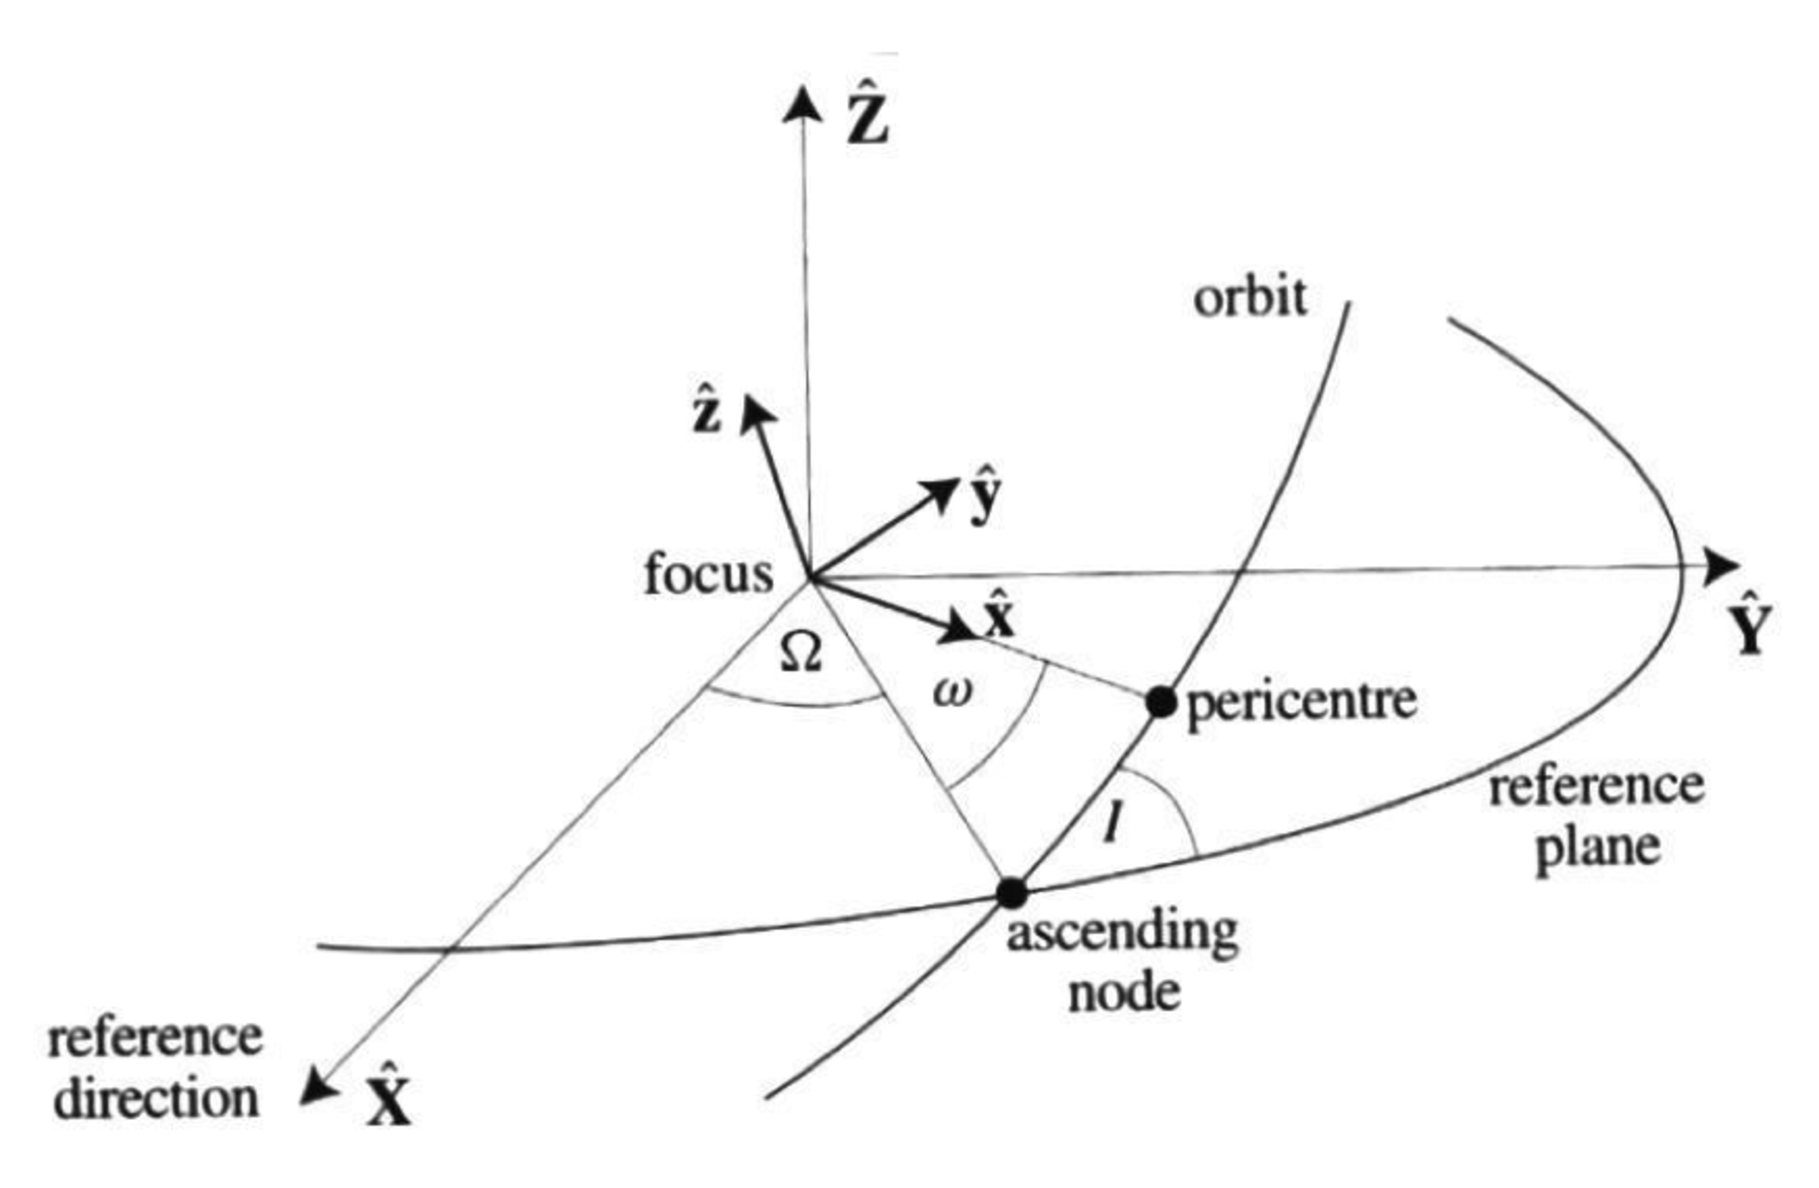
\includegraphics[width=10cm]{./image/sec2_13.pdf}
\caption{3次元空間での基準面に対する軌道運動.(Solar System Dynamics\cite{SSD} より引用)\label{fig:elements_SSD}}
\end{figure}

一般に軌道面は基準面に対して軌道傾斜角 (inclination,$I$) と呼ばれる角度だけ傾いている.軌道面と基準面が交わる線を交線 (line of nodes) と呼ぶ.基準面に対して下から上に軌道が横切る際の交点を昇交点 (ascending node),基準線と昇交点の動径ベクトルのなす角を昇交点経度 (longitude of ascending node,$\Omega$) と呼ぶ.昇交点の動径ベクトルと近点の方向のなす角を近日点引数 (argument of perisentre,$\omega$) と呼ぶ.

軌道傾斜角は常に $0 \leq I \leq 180^{\circ}$ である.$I \leq 90 ^{\circ}$ の場合は順行 (prograde),一方 $I \geq 90 ^{\circ}$ の場合は逆行 (retrograde) と呼ぶ.

$I \to 0$ の極限では軌道面は基準面と同一平面上に存在し,
\begin{equation}
\varpi = \Omega + \omega \label{eq:varpi}
\end{equation}
ここで $\varpi$ は\ref{sec:position&velocity}節で導入した近日点経度である.しかし $\Omega$ と $\omega$ は異なる平面上で定義される角度にも関わらず,式(\ref{eq:varpi})の $\varpi$ の定義は軌道が傾いている場合にも使われる.ゆえに,$\varpi$ は一般に "曲がった" 角 ("dogleg" angle) とも呼ばれる.

図\ref{fig:xyzXYZ}は軌道面の座標系と基準面の座標系の関係を示している.1つの座標系は,他の座標系を軸に沿って回転させることで表現できることがわかる.

軌道面の座標系 ($x, y, z$) から基準面の座標系 ($X, Y, Z$) へ変換するためには,(i) $x$ 軸が交線 (line of nodes) と一致するように $z$ 軸を中心に $\omega$ だけ回転させ,(ii) 次に2つの平面が一致するように $x$ 軸を中心に $I$ だけ回転させ,(iii) 最後に $z$ 軸を中心に $\Omega$ だけ回転させる (図\ref{fig:elements_SSD},\ref{fig:xyzXYZ},\ref{fig:grapher}参照).

\begin{figure}[H]
\centering
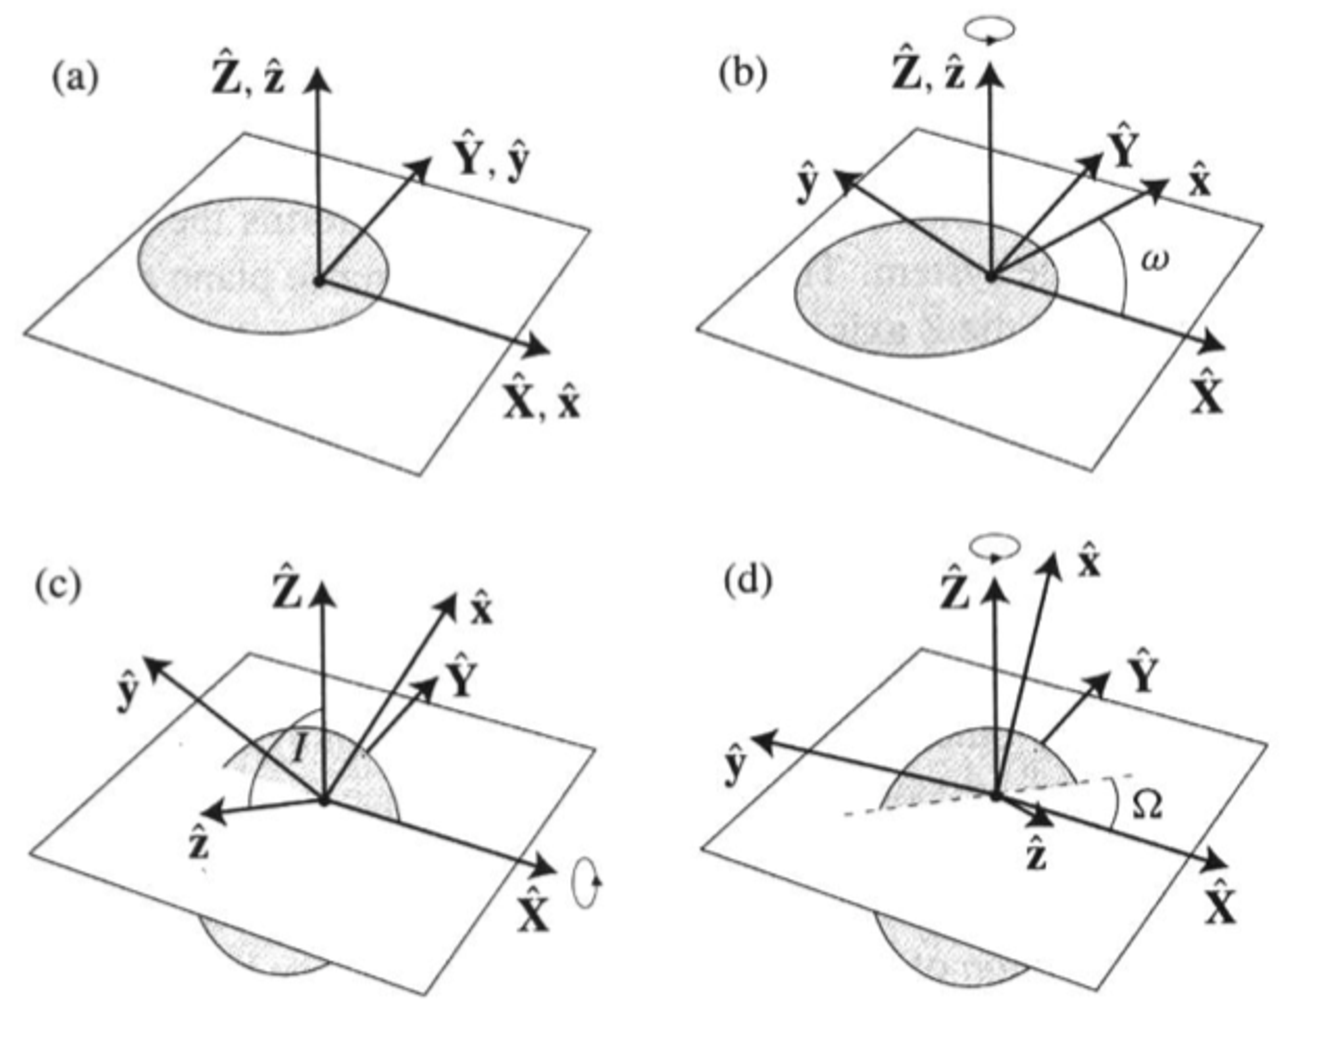
\includegraphics[width=10cm]{./image/sec2_14.pdf}
\caption{単位ベクトル $\hat{\bm x}, \hat{\bm y}, \hat{\bm z}, \hat{\bm X}, \hat{\bm Y}, \hat{\bm Z}$ と角度 $\omega, I, \Omega$ の関係.(a) 近日点の向きを $\hat{\bm X}$ 軸と一致させる.(b) まず $\hat{\bm Z}$ 軸正の向きに $\omega$ 回転させる.(c) 次に $\hat{\bm X}$ 軸正の向きに $I$ 回転させる.(d) 最後に $\hat{\bm Z}$ 軸正の向きに $\Omega$ 回転させる.(Solar System Dynamics\cite{SSD} より引用)\label{fig:xyzXYZ}}
\end{figure}

\begin{figure}[H]
\begin{tabular}{cc}
%左
\begin{minipage}[t]{0.45\hsize}
\centering
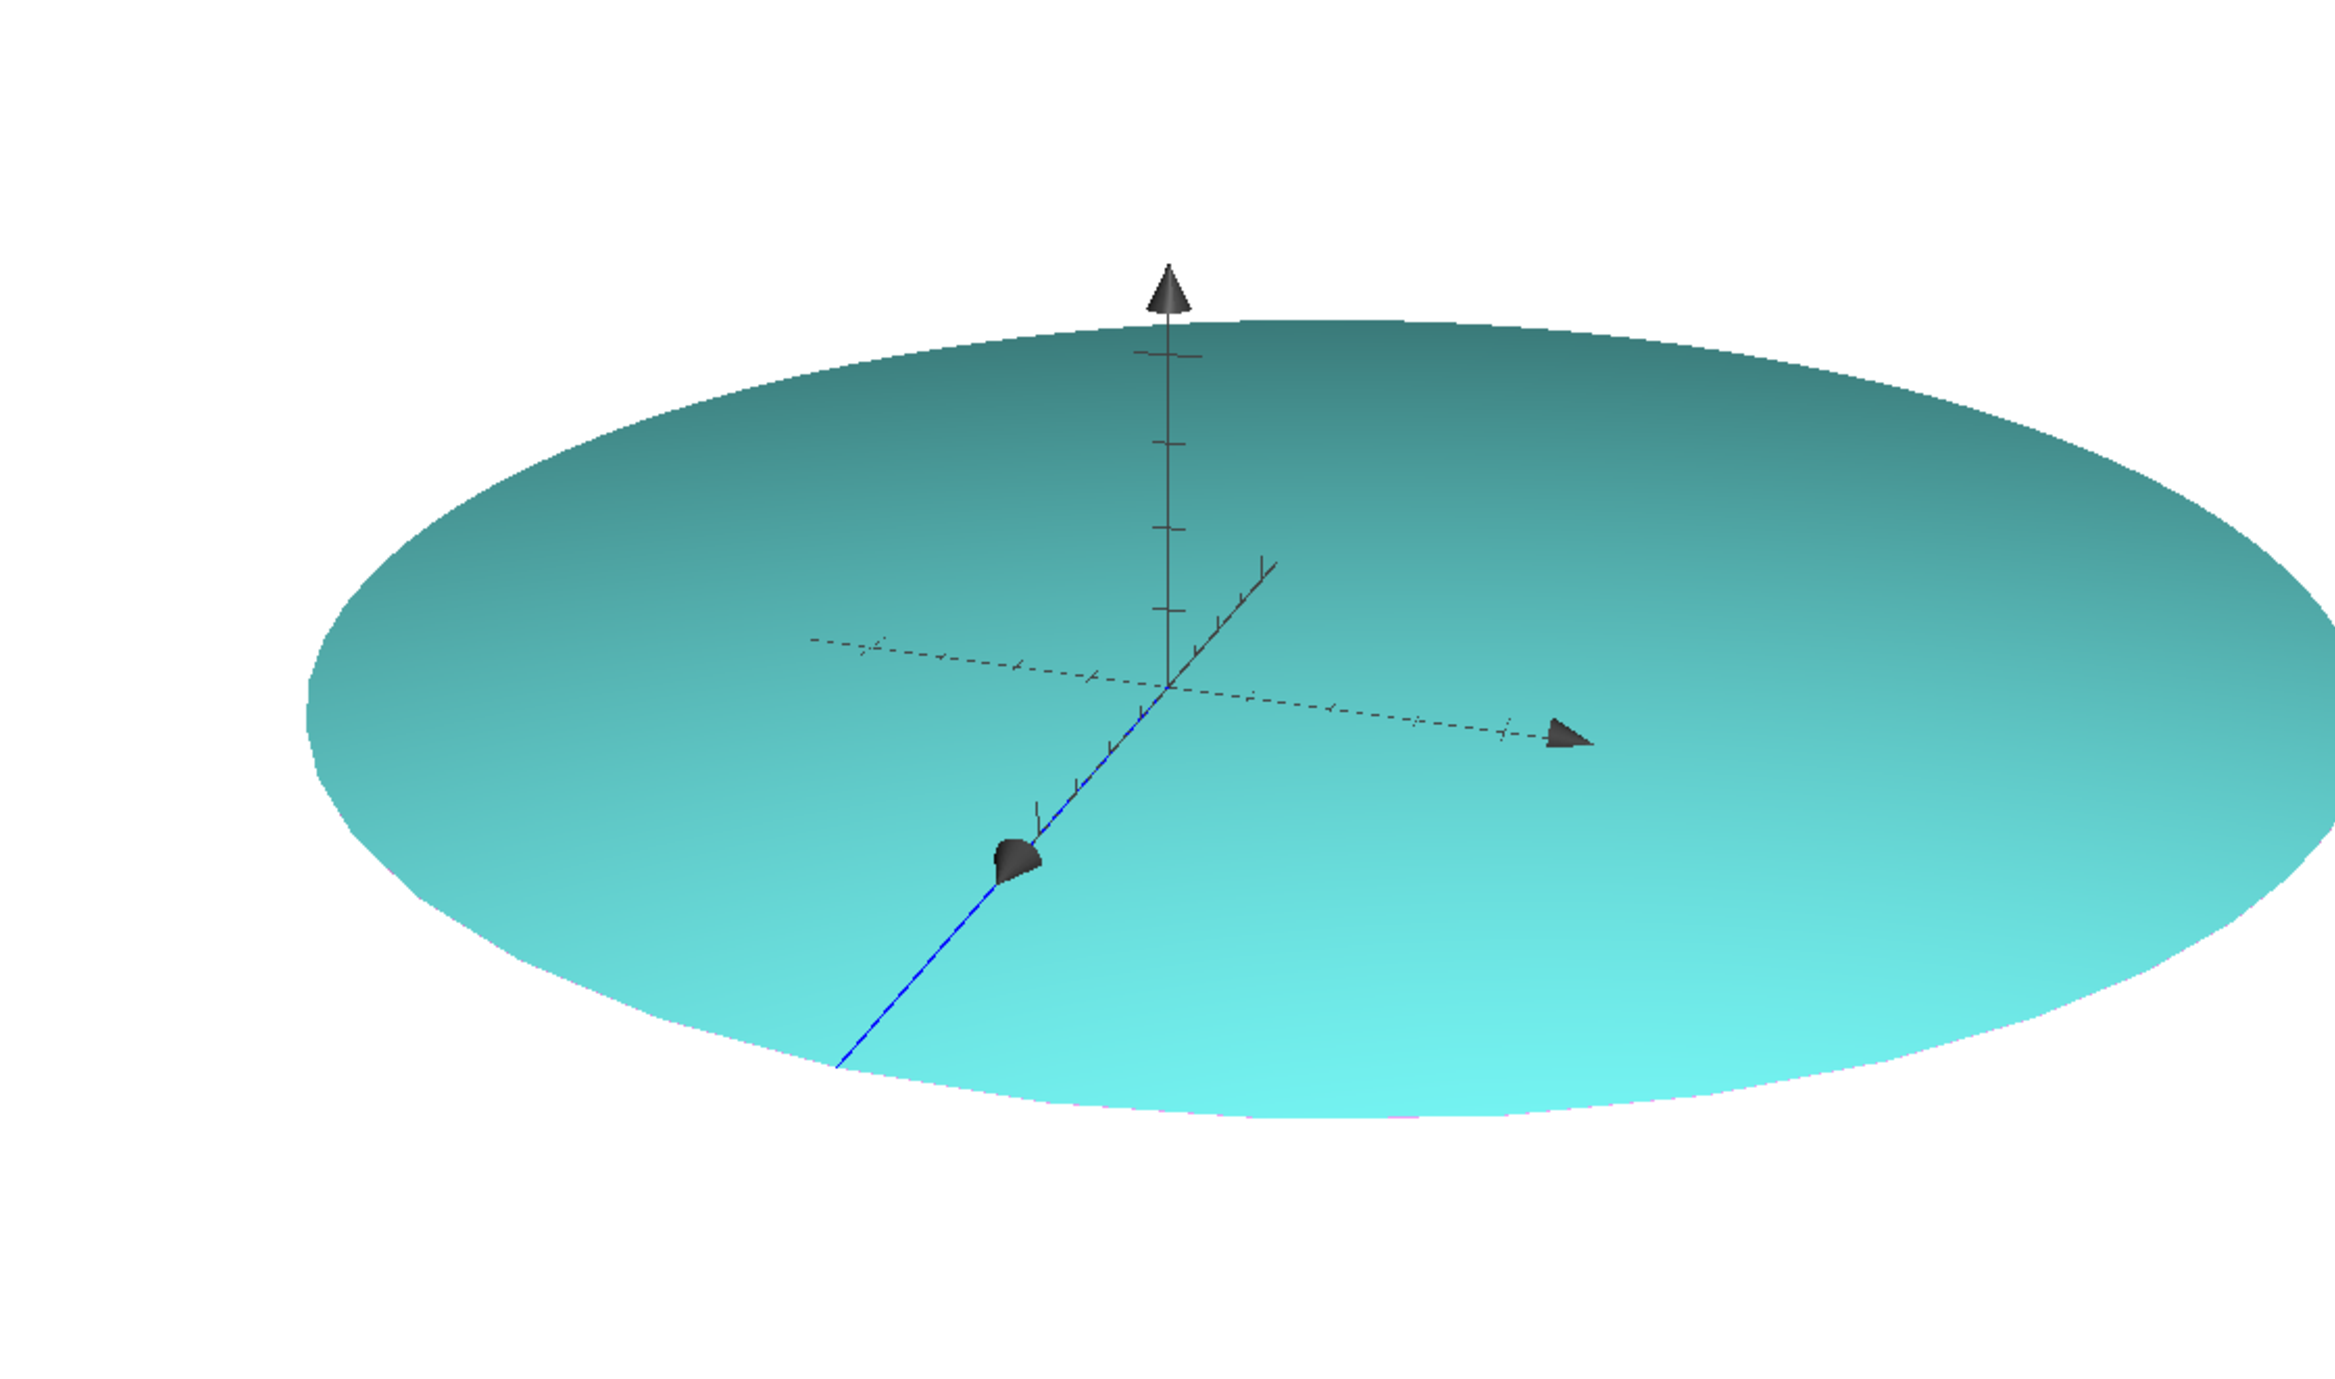
\includegraphics[width=7cm]{./image/ellipse1.pdf}
\end{minipage} &
%右
\begin{minipage}[t]{0.45\hsize}
\centering
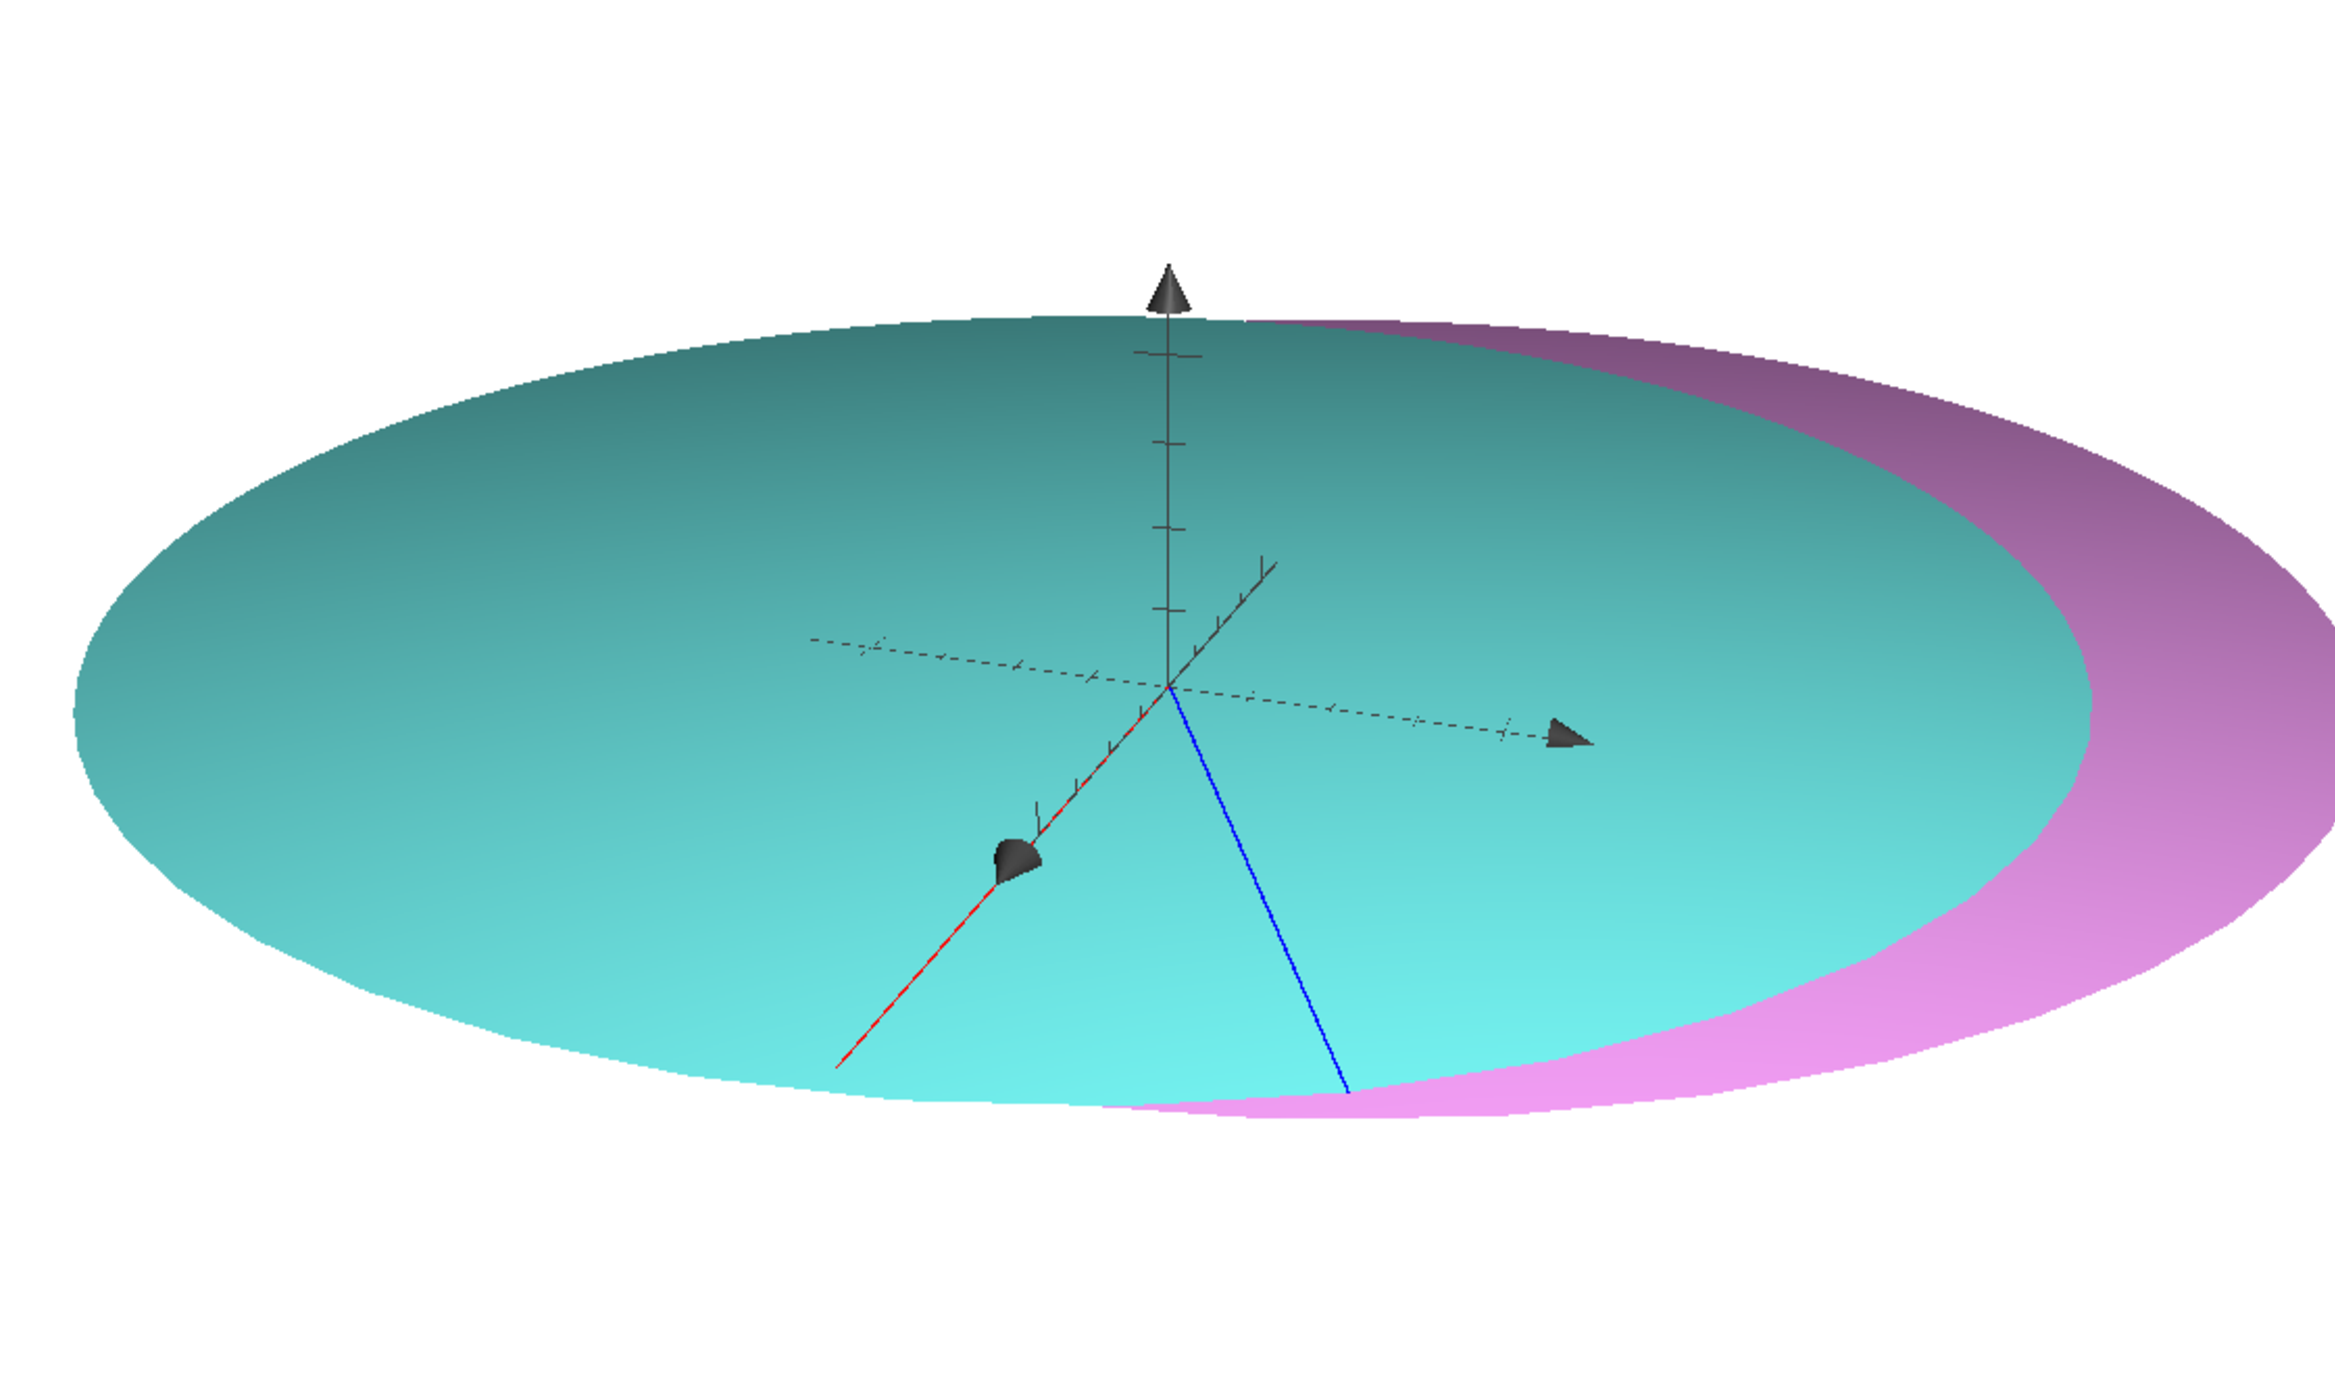
\includegraphics[width=7cm]{./image/ellipse2.pdf}
\end{minipage}\\
%
%左
\begin{minipage}[t]{0.45\hsize}
\centering
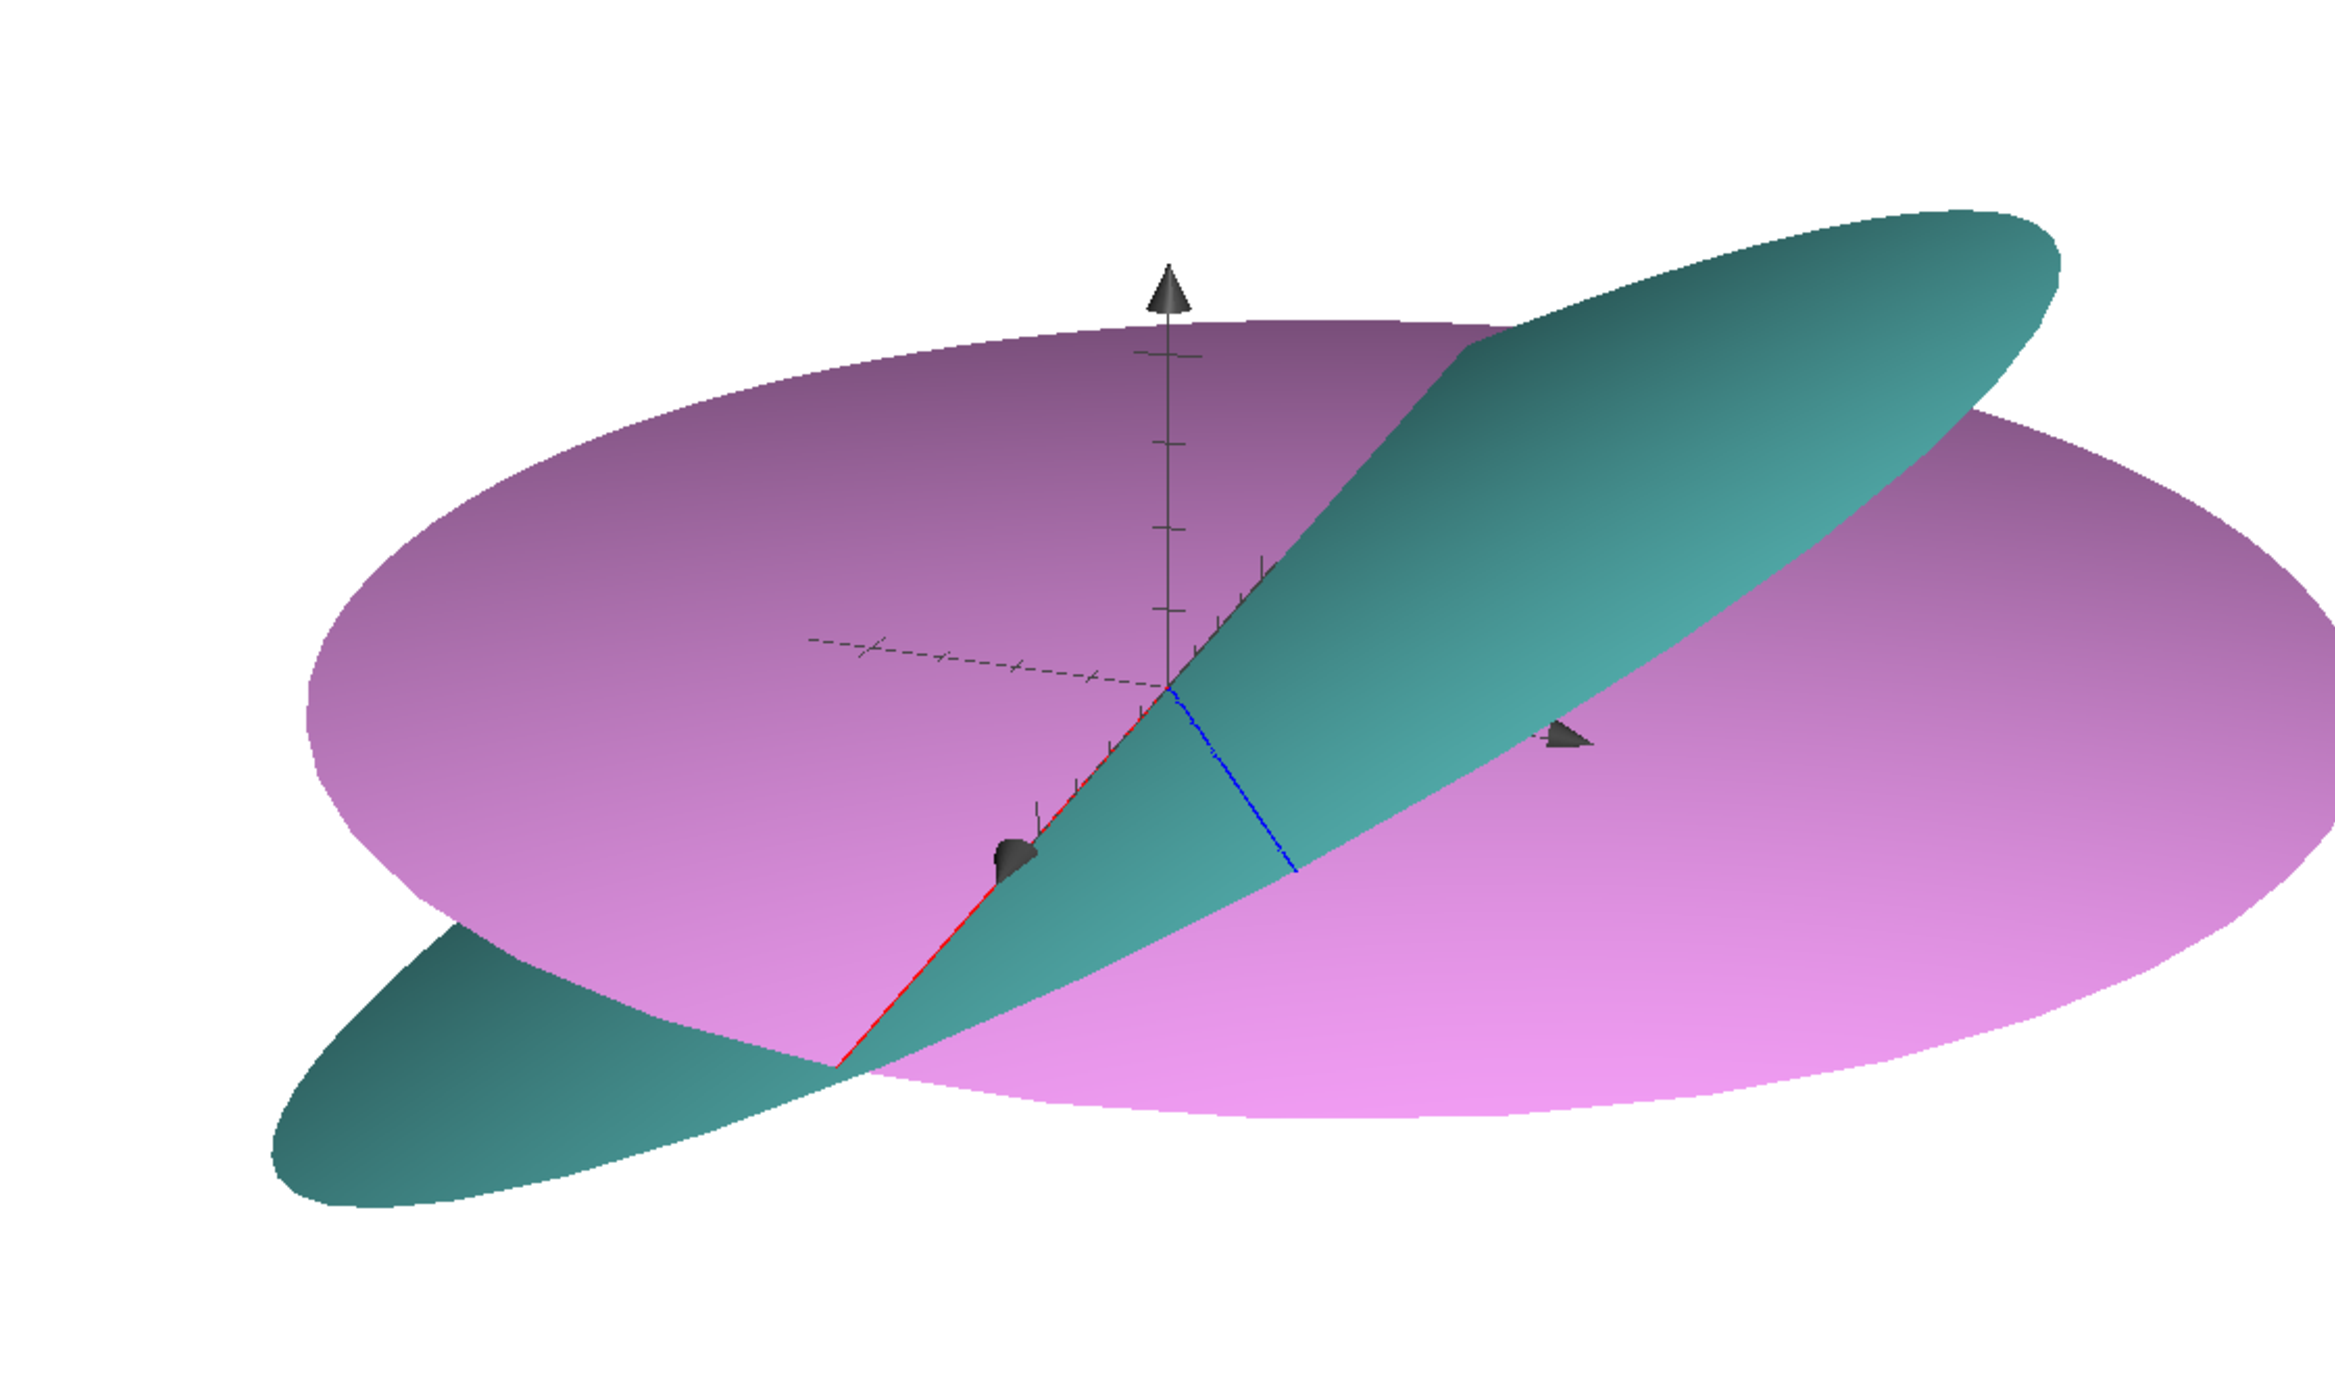
\includegraphics[width=7cm]{./image/ellipse3.pdf}
\end{minipage} &
%右
\begin{minipage}[t]{0.45\hsize}
\centering
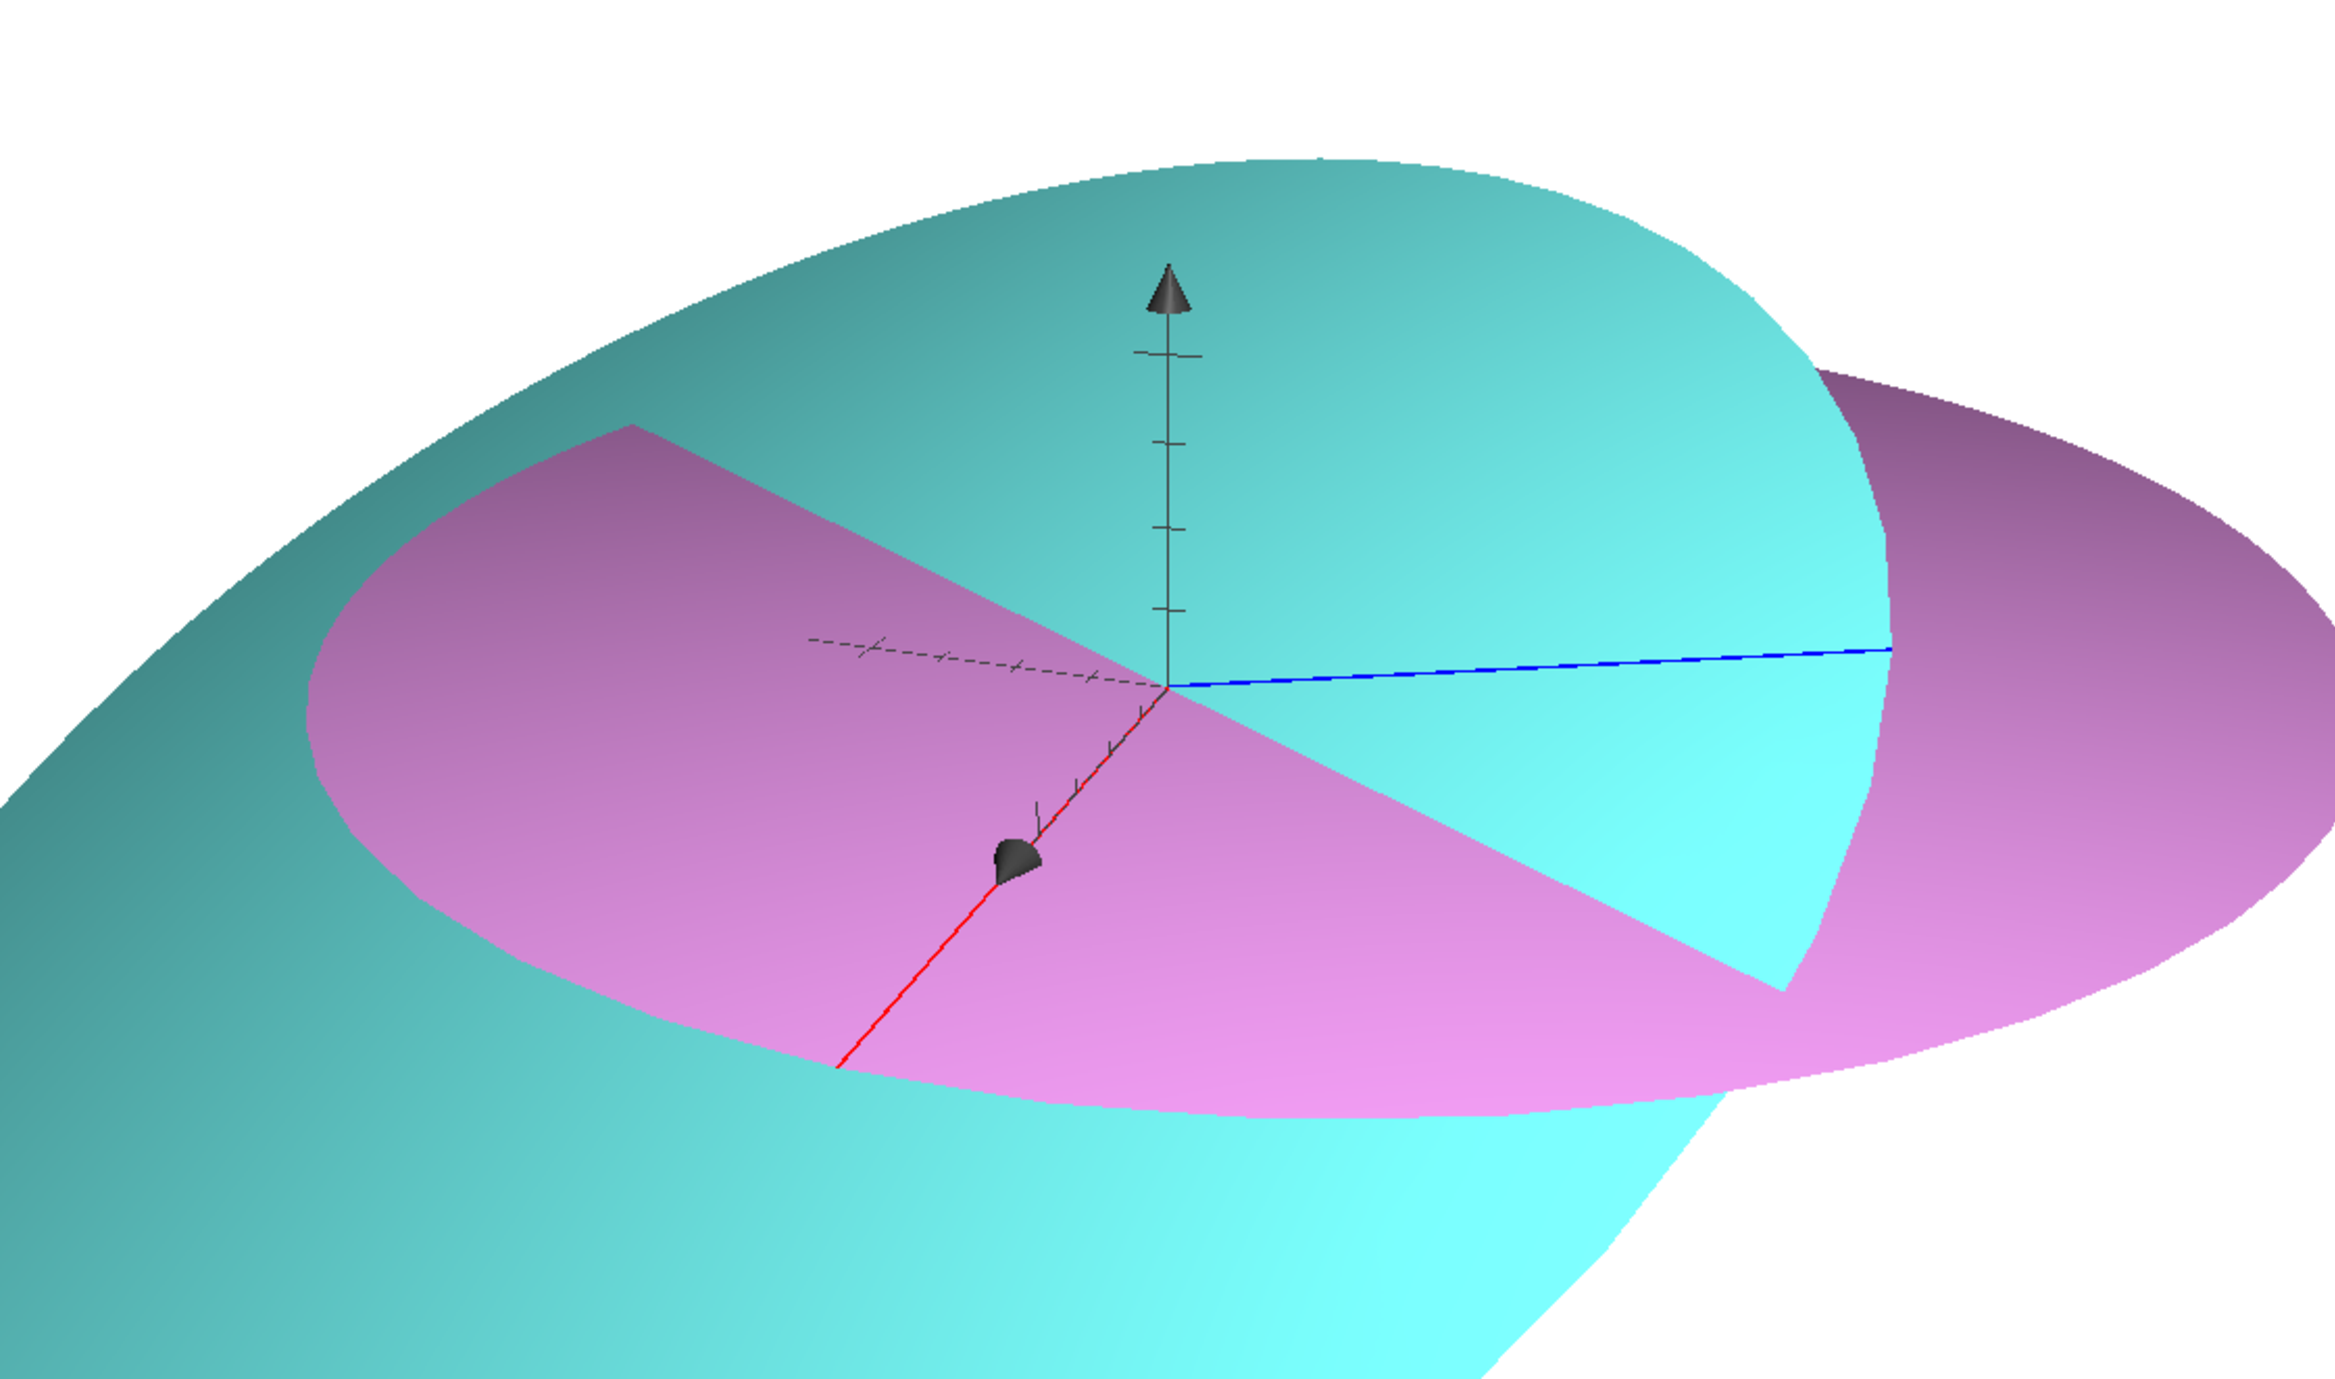
\includegraphics[width=7cm]{./image/ellipse4.pdf}
\end{minipage}
%
\end{tabular}
\caption{上と同じ操作をしたときの基準面(ピンク)と軌道面(水色).\label{fig:grapher}}
\end{figure}

これらのような3次元座標系の変換は,それぞれ ${\rm{\bm P}}_1,{\rm{\bm P}}_2,{\rm{\bm P}}_3$ のような3 $\times$ 3回転行列で表現できる.

\begin{equation}
{\rm{\bm P}}_1 =
\begin{pmatrix}
\cos \omega & - \sin \omega & 0\\
\sin \omega & \cos \omega & 0 \\
0 & 0 & 1\\
\end{pmatrix}
, \quad {\rm{\bm P}}_2 =
\begin{pmatrix}
1 & 0 & 0\\
0 & \cos I & - \sin I\\
0 & \sin I & \cos I\\
\end{pmatrix}
, \quad {\rm{\bm P}}_3 =
\begin{pmatrix}
\cos \Omega & - \sin \Omega & 0\\
\sin \Omega & \cos \Omega & 0 \\
0 & 0 & 1\\
\end{pmatrix}
\end{equation}

これらを使うと,
\begin{equation}
\begin{pmatrix}
X\\
Y\\
Z\\
\end{pmatrix}
= {\rm{\bm P}}_3 {\rm{\bm P}}_2 {\rm{\bm P}}_1
\begin{pmatrix}
x\\
y\\
z\\
\end{pmatrix}
\quad {\rm and} \quad
\begin{pmatrix}
x\\
y\\
z\\
\end{pmatrix}
= {\rm{\bm P}}_1^{-1} {\rm{\bm P}}_2^{-1} {\rm{\bm P}}_3^{-1}
\begin{pmatrix}
X\\
Y\\
Z\\
\end{pmatrix}
\end{equation}
ここで ${\rm{\bm P}}^{-1}$ は ${\rm{\bm P}}$ の逆行列である.すべての回転行列は直交行列であるため,逆行列は転置行列と等しい.

軌道面の座標系を基準面の座標系で表すと,
\begin{equation}
\begin{pmatrix}
X\\
Y\\
Z\\
\end{pmatrix}
= {\rm{\bm P}}_3 {\rm{\bm P}}_2 {\rm{\bm P}}_1
\begin{pmatrix}
r \cos f\\
r \sin f\\
0\\
\end{pmatrix}
= r 
\begin{pmatrix}
\cos \Omega \cos (\omega + f) - \sin \Omega \sin (\omega + f) \cos I\\
\sin \Omega \cos (\omega + f) + \cos \Omega \sin (\omega + f) \cos I\\
\sin (\omega + f) \sin I\\
\end{pmatrix}
\label{eq:xyzXYZ}
\end{equation}
回転変換では長さは保存されるため,$a, e$ の値は変化しない.

これで時間 $t$ での楕円運動をする天体の基準面の座標系における位置 ($X, Y, Z$) と速度 ($\dot{X}, \dot{Y}, \dot{Z}$) を,6つの軌道要素 $a, e, I, \Omega, \omega, f$ と近点通過時刻 $\tau$ に変換することができるようになった.中心星とそのまわりを回る天体の質量をそれぞれ $m_1, m_2$ とすると,
\begin{eqnarray}
R^2 & = & X^2 + Y^2 + Z^2, \label{eq:R}\\
V^2 & = & \dot{X}^2 + \dot{Y}^2 + \dot{Z}^2, \label{eq:Rdot}\\
{\bm R} \cdot \dot{{\bm R}} & = & X \dot{X} + Y \dot{Y} + Z \dot{Z}, \\
{\bm h} & = & (Y \dot{Z} - Z \dot{Y}, Z \dot{X} - X \dot{Z}, X \dot{Y} - Y \dot{X}), \\
\dot{R} & = & \pm \sqrt{V^2 - \frac{h^2}{R^2}}.
\end{eqnarray}
ここで $R = r$ は動径ベクトルの長さ,$\dot{R}$ はその変化率を示している.$R$ は常に正なので,$\dot{R}$ の符号は ${\bm R} \cdot \dot{{\bm R}}$ の符号と一致する.${\bm h} = (h_X, h_Y, h_Z)$ のそれぞれの成分は,
\begin{eqnarray}
h \cos I & = & h_Z, \label{eq:h_Z}\\
h \sin I \sin \Omega & = & \pm h_X, \label{eq:h_X}\\
h \sin I \cos \Omega & = & \mp h_Y. \label{eq:h_Y}
\end{eqnarray}
ここで,$h_Z$ の符号が正のとき式(\ref{eq:h_X}),式(\ref{eq:h_Y})の上の符号,$h_Z$ の符号が負のとき下の符号をとる.

軌道要素を求める過程を以下に示す.

\begin{description}
\item[1)] 式(\ref{eq:v2new}),式(\ref{eq:R}),式(\ref{eq:Rdot})から $a$ を求める.
\begin{equation}
a = \left( \frac{2}{R} -\frac{V^2}{G (m_1 + m_2)} \right)^{-1} \label{eq:axis}
\end{equation}
\item[2)] 式(\ref{eq:mu}),式(\ref{eq:axis})から $e$ を求める.
\begin{equation}
e = \sqrt{1- \frac{h^2}{G (m_1 + m_2) a}} \label{eq:ecc}
\end{equation}
\item[3)] 式(\ref{eq:h_Z})から $I$ を求める.
\begin{equation}
I = \cos^{-1} \left( \frac{h_Z}{h} \right) \label{eq:inc}
\end{equation}
\item[4)] 式(\ref{eq:h_X}),式(\ref{eq:h_Y})から $\sin \Omega,\cos \Omega$ の形で $\Omega$ を求める.
\begin{equation}
\sin \Omega = \frac{\pm h_X}{h \sin I} \quad {\rm and} \quad \cos \Omega = \frac{\mp h_Y}{h \sin I}. \label{eq:OMEGA}
\end{equation}
符号は $h_Z$ の符号によって決まる.
\item[5)] 式(\ref{eq:xyzXYZ})の $Z/R, X/R$ の表式から $\omega + f$ を求める.
\begin{equation}
\sin (\omega + f) = \frac{Z}{R \sin I} \quad {\rm and} \quad \cos (\omega + f) = \frac{1}{\cos \Omega} \left( \frac{X}{R} + \sin \Omega \sin (\omega + f) \cos I \right). \label{eq:omega+f}
\end{equation}
\item[6)] 式(\ref{eq:rf}),式(\ref{eq:rdot})から得られる $\sin f$ と $\cos f$ の表式から $f, \omega$ を求める.$\dot{r} = \dot{R}$ と置き換えると,
\begin{equation}
\sin f = \frac{a (1 - e^2)}{h e} \dot{R} \quad {\rm and} \quad \cos f = \frac{1}{e} \left( \frac{a (1 - e^2)}{R} - 1 \right). \label{eq:f}
\end{equation}
\item[7)] 式(\ref{eq:rE})から $E$を計算し,式(\ref{eq:mu}),式(\ref{eq:tauE})を用いて $\tau$ を求める.
\begin{equation}
\tau = t - \frac{E - e \sin E}{\sqrt{G (m_1 + m_2) a^{-3}}} \label{eq:tau}
\end{equation}
\end{description}

これらの式は軌道要素を求める正しい方法であるが,数値計算において,SI単位系や他の標準的な単位系よりも実用的な単位系を用いて,$G (m_1 + m_2) = 1$ とするように,すなわち時間 $t$ を $\sqrt{\mu} = \sqrt{G (m_1 + m_2)}$ でスケーリングし, 新たな時間 $\bar{t}$ を用いることがある.
\begin{equation}
\sqrt{\mu} dt = d \bar{t} \label{eq:tbar}
\end{equation}

式(\ref{eq:raletive})から,これは $\mu = 1$ としたときと同じである.加えて,単位長さを $a = 1$ と選ぶと,2体問題は単位平均運動 $n = 1$ と単位周期 $T = 2 \pi$ のケプラー運動として扱うことができる.これは円制限3体問題を扱う際にも同様の形で適用できる.


\section{制限3体問題 \label{sec:3body}}
この節では3体の物体が重力相互作用をした場合に拡張して考える.特に,3体目の質量が他の2つに比べ無視できるほど小さいときの3体目の物体の運動について考える.この問題は「制限3体問題」と呼ばれる.また,1,2体目の物体がそれらの共通重心を中心に円運動をし,3体目の物体がそれと同一な平面上を運動する場合,「円制限3体問題」と呼ばれる.一見すると,太陽系の天体運動に対して円制限3体問題はほとんど応用できないと思えるかもしれない.観測された太陽系の天体はやはり,同一平面上を運動せず円運動もしていない.しかし,太陽系の天体の軌道と質量の階層構造 (太陽,惑星,衛星,リングなど) は,制限3体問題がよい近似であり,比較的簡単な解析で定性的に天体の運動の振る舞いを理解できることを示している.

\subsection{運動方程式}
2つの質量 $m_1, m_2$ の物体の重力の影響下で,質量が無視できるほど小さい粒子の運動を考える.粒子は2つの物体に影響を与えないが,2つの物体は共通重心を中心に円運動をして粒子に力を及ぼすと仮定する.

$\xi, \eta, \zeta$ の軸を持ち,2つの物体の重心を原点にとる慣性座標系を考える (図\ref{fig:xi_eta_zeta}).時刻 $t = 0$ で $m_1$ から $m_2$ に沿った方向に $\xi$ 軸,軌道平面上で $\xi$ 軸と垂直な方向に $\eta$ 軸,そして $\xi - \eta$ 平面に垂直な,角運動量ベクトルの方向に $\zeta$ 軸をとる.この慣性座標系での2つの物体の座標を ($\xi_1, \eta_1, \zeta_1$) ,($\xi_2, \eta_2, \zeta_2$) とし,距離は一定で,同じ角速度で共通重心のまわりを回っているとする.また単位質量を $\mu = G (m_1 + m_2) = 1$ となるように選ぶ.$m_1 > m_2$ と仮定し,
\begin{equation}
\bar{\mu} = \frac{m_2}{m_1 + m_2}
\end{equation}
と定義すると,この単位系での2つの物体の質量は,
\begin{equation}
\mu_1 = G m_1 = 1 - \bar{\mu} \quad {\rm and} \quad \mu_2 = G m_2 = \bar{\mu}, \label{eq:mu1mu2}
\end{equation}
となり,ここで仮定より $\bar{\mu} < 1/2$ である.単位長さは,2つの物体間の距離が1となるように選ぶ.そうすると,共通の平均運動 $n$ も1となる.

\begin{figure}[H]
\centering
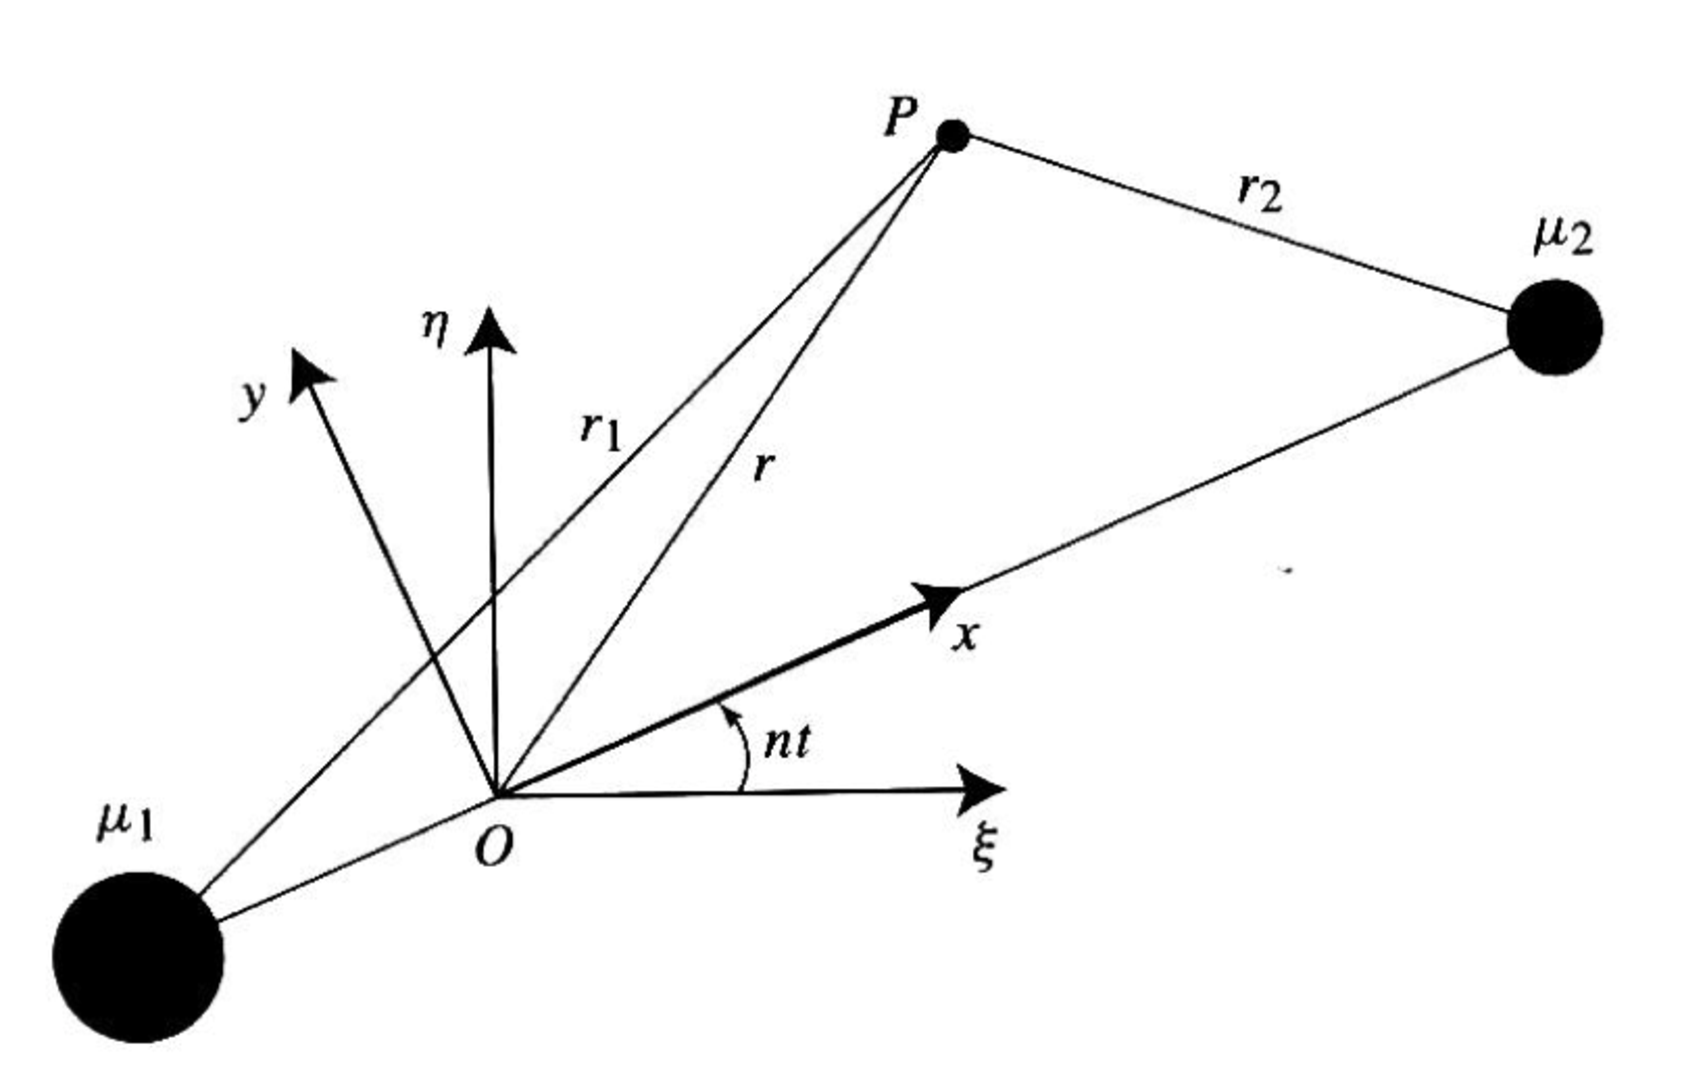
\includegraphics[width=10cm]{./image/sec3_1.pdf}
\caption{sidereal 座標系 ($\xi, \eta, \zeta$) とsynodic座標系 ($x, y, z$) の関係.点 $P$ は粒子.原点 $O$ は2つの物体の重心に位置する.$\zeta$ 軸と $z$ 軸は回転軸と一致する.矢印は正の回転の向きを表す.(Solar System Dynamics\cite{SSD} より引用)\label{fig:xi_eta_zeta}}
\end{figure}

慣性座標系,すなわちsidereal座標系での粒子の座標を ($\xi, \eta, \zeta$) とする.逆2乗則のベクトル形式を用いると,
粒子の運動方程式は,
\begin{eqnarray}
\ddot{\xi} & = & \mu_1 \frac{\xi_1 - \xi}{r_1^3} + \mu_2 \frac{\xi_2 - \xi}{r_2^3}, \label{eq:xiddot}\\
\ddot{\eta} & = & \mu_1 \frac{\eta_1 - \eta}{r_1^3} + \mu_2 \frac{\eta_2 - \eta}{r_2^3}, \label{eq:etaddot}\\
\ddot{\zeta} & = & \mu_1 \frac{\zeta_1 - \zeta}{r_1^3} + \mu_2 \frac{\zeta_2 - \zeta}{r_2^3}, \label{eq:zetaddot}
\end{eqnarray}
となり,ここで図\ref{fig:xi_eta_zeta}より,
\begin{eqnarray}
r_1^2 & = & (\xi_1 - \xi)^2 + (\eta_1 - \eta)^2 + (\zeta_1 - \zeta)^2,\\
r_2^2 & = & (\xi_2 - \xi)^2 + (\eta_2 - \eta)^2 + (\zeta_2 - \zeta)^2.
\end{eqnarray}
これらの方程式は,2つの物体の軌道の仮定が必要ないため,一般の3体問題にも有効である.

2つの物体が円運動をするとき,それらの距離と平均運動は一定である.このような場合,2つの物体の位置も固定されるような回転座標系での粒子の運動を考えたほうが自然である.ここで,$\xi, \eta$ 座標と原点は同じだが,正の方向に一定の回転速度 $n$ で回転する新たな座標系を考える (図\ref{fig:xi_eta_zeta}).$x$ 軸を2つの物体に沿うようにとると,それぞれの座標は ($x_1, y_1,z_1$) = ($- \mu_2, 0, 0$),($x_2, y_2, z_2$) = ($\mu_1, 0, 0$) である.したがって,式(\ref{eq:mu1mu2})と図\ref{fig:xi_eta_zeta} より,
\begin{eqnarray}
r_1^2 & = & (x + \mu_2)^2 + y^2 + z^2,\\
r_2^2 & = & (x - \mu_1)^2 + y^2 + z^2,
\end{eqnarray}
となり,ここで ($x, y, z$) は回転座標系,すなわちsynodic座標系での粒子の座標である.これらの座標系は次のような単純な回転で関連づけられる.
\begin{equation}
\begin{pmatrix}
\xi\\
\eta\\
\zeta\\
\end{pmatrix}
= 
\begin{pmatrix}
\cos nt & - \sin nt & 0\\
\sin nt & \cos nt & 0\\
0 & 0 & 1\\
\end{pmatrix}
\begin{pmatrix}
x\\
y\\
z\\
\end{pmatrix}. \label{eq:xi_eta_zeta_x_y_z}
\end{equation}
今用いている単位系では $n = 1$ であるが,方程式中に $n$ をあえて残しておく.

式(\ref{eq:xi_eta_zeta_x_y_z})を各成分ごとに2階微分すると,
\begin{equation}
\begin{pmatrix}
\dot{\xi}\\
\dot{\eta}\\
\dot{\zeta}\\
\end{pmatrix}
= 
\begin{pmatrix}
\cos nt & - \sin nt & 0\\
\sin nt & \cos nt & 0\\
0 & 0 & 1\\
\end{pmatrix}
\begin{pmatrix}
\dot{x} - ny\\
\dot{y} + nx\\
\dot{z}\\
\end{pmatrix} \label{eq:xidot_etadot_zetadot}
\end{equation}

\begin{equation}
\begin{pmatrix}
\ddot{\xi}\\
\ddot{\eta}\\
\ddot{\zeta}\\
\end{pmatrix}
= 
\begin{pmatrix}
\cos nt & - \sin nt & 0\\
\sin nt & \cos nt & 0\\
0 & 0 & 1\\
\end{pmatrix}
\begin{pmatrix}
\ddot{x} - 2 n \dot{y} - n^2 x\\
\ddot{y} + 2 n \dot{x} - n^2 y\\
\ddot{z}\\
\end{pmatrix}. \label{eq:xiddot_etaddot_zetaddot}
\end{equation}
回転座標系に切り替えることによって,$n \dot{x}, n \dot{y}$ の項 (コリオリ力) と $n^2 x, n^2 y$ の項 (遠心力) が運動方程式に生じる.これらの式を使って式(\ref{eq:xiddot}),式(\ref{eq:etaddot}),式(\ref{eq:zetaddot})を書き換えると,
\begin{equation}
\begin{split}
(\ddot{x} - 2 n \dot{y} & - n^2 x) \cos nt - (\ddot{y} + 2 n \dot{x} - n^2 y) \sin nt =\\
& \left[ \mu_1 \frac{x_1 - 1}{r_1^3} + \mu_2 \frac{x_2 - x}{r_2^3} \right] \cos nt + \left[ \frac{\mu_1}{r_1^3} + \frac{\mu_2}{r_2^3} \right] y \sin nt, \label{eq:cos_sin}
\end{split}
\end{equation}
\begin{equation}
\begin{split}
(\ddot{x} - 2 n \dot{y} & - n^2 x) \sin nt + (\ddot{y} + 2 n \dot{x} - n^2 y) \cos nt =\\
& \left[ \mu_1 \frac{x_1 - 1}{r_1^3} + \mu_2 \frac{x_2 - x}{r_2^3} \right] \sin nt - \left[ \frac{\mu_1}{r_1^3} + \frac{\mu_2}{r_2^3} \right] y \cos nt, \label{eq:sin_cos}
\end{split}
\end{equation}
\begin{equation}
\ddot{z} = - \left[ \frac{\mu_1}{r_1^3} + \frac{\mu_2}{r_2^3} \right] z.
\end{equation}
式(\ref{eq:cos_sin})と $\cos nt$ の積,式(\ref{eq:sin_cos})と $\sin nt$ の積の和をとり,また式(\ref{eq:cos_sin})と $- \sin nt$ の積,式(\ref{eq:sin_cos})と $\cos nt$ の積の和をとると,synodic座標系での運動方程式は,
\begin{eqnarray}
\ddot{x} - 2 n \dot{y} - n^2 x & = & - \left[ \mu_1 \frac{x + \mu_2}{r_1^3} + \mu_2 \frac{x - \mu_1}{r_2^3} \right],\\
\ddot{y} + 2 n \dot{x} - n^2 y & = & - \left[ \frac{\mu_1}{r_1^3} + \frac{\mu_2}{r_2^3} \right] y,\\
\ddot{z} & = & - \left[ \frac{\mu_1}{r_1^3} + \frac{\mu_2}{r_2^3} \right] z.
\end{eqnarray}
これらの運動方程式はスカラー関数 $U$ の勾配として書くこともできる.
\begin{eqnarray}
\ddot{x} - 2 n \dot{y} & = & \frac{\partial U}{\partial x}, \label{eq:xU}\\
\ddot{y} + 2 n \dot{x} & = & \frac{\partial U}{\partial y}, \label{eq:yU}\\
\ddot{z} & = & \frac{\partial U}{\partial z}. \label{eq:zU}
\end{eqnarray}
ここで $U = U (x, y, z)$ は次のように与えられる.
\begin{equation}
U = \frac{n^2}{2} (x^2 + y^2) + \frac{\mu_1}{r_1} + \frac{\mu_2}{r_2}. \label{eq:U}
\end{equation}
$x^2 + y^2$ の項は遠心力によるポテンシャル,$1/r_1, 1/r_2$ の項は重力によるポテンシャルであり,それぞれの偏微分をとると運動方程式に遠心力,重力の項が現れる.

式(\ref{eq:xU}),式(\ref{eq:yU})の $- 2n \dot{y}$ と $+ 2n \dot{x}$ の項はコリオリ項であり,回転座標系での粒子の速度に依存する.コリオリ力は速度方向に対して右側にずれる力であり,ゆえに効かない.

$U$ の定義より符号は正であるが,単に天文学の伝統であり,物理では慣習として符号を負にする.$U^{\ast} = - U$ のように置き換えると運動方程式は,
\begin{eqnarray}
\ddot{x} - 2 n \dot{y} & = & - \frac{\partial U^{\ast}}{\partial x}, \label{eq:xUast}\\
\ddot{y} + 2 n \dot{x} & = & - \frac{\partial U^{\ast}}{\partial y}, \label{eq:yUast}\\
\ddot{z} & = & - \frac{\partial U^{\ast}}{\partial z}. \label{eq:zUast}
\end{eqnarray}
また,$U$ は真のポテンシャルではなく,回転座標系での粒子にかかる力のいくつか (全てではない) を得ることができるスカラー関数である.$U$ は偽ポテンシャルと呼ぶ.

\subsection{ヤコビ積分}
式(\ref{eq:xU})と $\dot{x}$ の積,式(\ref{eq:yU})と $\dot{y}$ の積,式(\ref{eq:zU})と $\dot{z}$ の積の和をとると,
\begin{equation}
\dot{x} \ddot{x} + \dot{y} \ddot{y} + \dot{z} \ddot{z} = \frac{\partial U}{\partial x} \dot{x} + \frac{\partial U}{\partial y} \dot{y} + \frac{\partial U}{\partial z} \dot{z} = \frac{dU}{dt}.
\end{equation}
これは積分できて,
\begin{equation}
\dot{x}^2 + \dot{y}^2 + \dot{z}^2 = 2 U - C_J, \label{eq:2U-C_J}
\end{equation}
ここで $C_J$ は積分定数である.$\dot{x}^2 + \dot{y}^2 + \dot{z}^2 = v^2$ は回転座標系での速度の2乗なので,
\begin{equation}
v^2 = 2 U - C_J
\end{equation}
または,式(\ref{eq:U})を用いて,
\begin{equation}
C_J = n^2 (x^2 + y^2) + 2 \left( \frac{\mu_1}{r_1} + \frac{\mu_2}{r_2} \right) - \dot{x}^2 - \dot{y}^2 - \dot{z}^2.
\end{equation}
これらのことから,$2 U - C_J$ はこの運動における定数であることがわかる.これはヤコビ積分,またはヤコビ定数であり,時には相対エネルギー積分とも呼ばれる.ただし,制限3体問題ではエネルギーも角運動量も保存しないので,エネルギー積分ではないことに注意する.ヤコビ積分は単に円制限3体問題における積分定数であり,これは一般の場合には3体問題は閉じた式で解くことはできないことを意味する.

$C_J$ の表式は,回転していない,sidereal座標系での粒子の位置と速度を使って書くこともできる.位置ベクトルは,式(\ref{eq:xi_eta_zeta_x_y_z})を用いると,
\begin{equation}
\begin{pmatrix}
x\\
y\\
z\\
\end{pmatrix}
= 
\begin{pmatrix}
\cos nt & \sin nt & 0\\
- \sin nt & \cos nt & 0\\
0 & 0 & 1\\
\end{pmatrix}
\begin{pmatrix}
\xi\\
\eta\\
\zeta\\
\end{pmatrix}. \label{eq:x_y_z_xi_eta_zeta}
\end{equation}
速度ベクトルは,式(\ref{eq:xidot_etadot_zetadot})を用いると,
\begin{equation}
\begin{pmatrix}
\dot{x} - ny\\
\dot{y} + nx\\
\dot{z}\\
\end{pmatrix}
= 
\begin{pmatrix}
\cos nt & \sin nt & 0\\
- \sin nt & \cos nt & 0\\
0 & 0 & 1\\
\end{pmatrix}
\begin{pmatrix}
\dot{\xi}\\
\dot{\eta}\\
\dot{\zeta}\\
\end{pmatrix} \label{eq:xdot_ydot_zdot_1}
\end{equation}
しかし,
\begin{equation}
\begin{pmatrix}
\dot{x} - ny\\
\dot{y} + nx\\
\dot{z}\\
\end{pmatrix}
= 
\begin{pmatrix}
\dot{x}\\
\dot{y}\\
\dot{z}\\
\end{pmatrix}
+ n
\begin{pmatrix}
\sin nt & - \cos nt & 0\\
\cos nt & \sin nt & 0\\
0 & 0 & 0\\
\end{pmatrix}
\begin{pmatrix}
\xi\\
\eta\\
\zeta\\
\end{pmatrix} \label{eq:xdot_ydot_zdot_2}
\end{equation}
とも書けるから,したがって,
\begin{equation}
\begin{pmatrix}
\dot{x}\\
\dot{y}\\
\dot{z}\\
\end{pmatrix}
= 
\begin{pmatrix}
\cos nt & \sin nt & 0\\
- \sin nt & \cos nt & 0\\
0 & 0 & 1\\
\end{pmatrix}
\begin{pmatrix}
\dot{\xi}\\
\dot{\eta}\\
\dot{\zeta}\\
\end{pmatrix}
- n
\begin{pmatrix}
\sin nt & - \cos nt & 0\\
\cos nt & \sin nt & 0\\
0 & 0 & 0\\
\end{pmatrix}
\begin{pmatrix}
\xi\\
\eta\\
\zeta\\
\end{pmatrix} \label{eq:xdot_ydot_zdot_3}
\end{equation}
ここで,
\begin{equation}
{\rm A} = 
\begin{pmatrix}
\cos nt & \sin nt & 0\\
- \sin nt & \cos nt & 0\\
0 & 0 & 1\\
\end{pmatrix}
 \quad {\rm and} \quad 
 {\rm B} = 
\begin{pmatrix}
\sin nt & - \cos nt & 0\\
\cos nt & \sin nt & 0\\
0 & 0 & 0\\
\end{pmatrix}
\end{equation}
とおくと,式(\ref{eq:xdot_ydot_zdot_3})から,
\begin{equation}
\begin{split}
\dot{x}^2 + \dot{y}^2 + \dot{z}^2 & = 
\begin{pmatrix}
\dot{x} & \dot{y} & \dot{z}\\
\end{pmatrix}
\begin{pmatrix}
\dot{x}\\
\dot{y}\\
\dot{z}\\
\end{pmatrix}\\
& = 
\begin{pmatrix}
\dot{\xi} & \dot{\eta} & \dot{\zeta}\\
\end{pmatrix}
{\rm A}^{\rm T} {\rm A} 
\begin{pmatrix}
\dot{\xi}\\
\dot{\eta}\\
\dot{\zeta}\\
\end{pmatrix}
- n
\begin{pmatrix}
\dot{\xi} & \dot{\eta} & \dot{\zeta}\\
\end{pmatrix}
{\rm A}^{\rm T} {\rm B} 
\begin{pmatrix}
\xi\\
\eta\\
\zeta\\
\end{pmatrix}\\
& \quad - n
\begin{pmatrix}
\xi & \eta & \zeta\\
\end{pmatrix}
{\rm B}^{\rm T} {\rm A}
 \begin{pmatrix}
\dot{\xi}\\
\dot{\eta}\\
\dot{\zeta}\\
\end{pmatrix}
+ n^2 
\begin{pmatrix}
\xi & \eta & \zeta\\
\end{pmatrix}
{\rm B}^{\rm T} {\rm B}
\begin{pmatrix}
\xi\\
\eta\\
\zeta\\
\end{pmatrix}\\
& =  \dot{\xi}^2 + \dot{\eta}^2 + \dot{\zeta}^2 + n^2 (\xi^2 + \eta^2) + 2 n (\dot{\xi} \eta - \dot{\eta} \xi)
\end{split}
\end{equation}
ここで,${\rm A}^{\rm T}, {\rm B}^{\rm T}$ は ${\rm A}, {\rm B}$ の転置行列を表す.${\rm A}, {\rm B}$ はどちらも直交行列なので,逆行列は単純に自身の転置行列である.回転行列を作用させても距離は常に変わらないので (言い換えると,直交行列の行列式は$\pm 1$なので),$x^2 + y^2 + z^2 = \xi^2 + \eta^2 + \zeta^2$ である.このことは,式(\ref{eq:xi_eta_zeta_x_y_z})からも得られる.したがって,sidereal座標系でのヤコビ積分の表式は,
\begin{equation}
C_J = 2 \left( \frac{\mu_1}{r_1} + \frac{\mu_2}{r_2} \right) + 2 n (\dot{\xi} \eta - \dot{\eta} \xi) - \dot{\xi}^2 - \dot{\eta}^2 - \dot{\zeta}^2 \label{eq:C_J}
\end{equation}
となる.これは以下のように書き直せる.
\begin{equation}
 \frac{1}{2} (\dot{\xi}^2 + \dot{\eta}^2 + \dot{\zeta}^2) - \left( \frac{\mu_1}{r_1} + \frac{\mu_2}{r_2} \right) = {\bm h} \cdot {\bm n} - \frac{1}{2} C_J
\end{equation}
ここで ${\bm n} = (0, 0, n)$ であり,左辺は粒子の単位質量あたりの全エネルギーである.${\bm h} \cdot {\bm n}$ は一定ではないため,制限3体問題ではエネルギーが保存しない理由はこの式で説明できる.

各座標系での粒子の位置と速度を測定することで,粒子の運動と関連したヤコビ積分の値を決定することができる.2体問題では,角運動量とエネルギー積分を使って相対運動を解くことができた.ヤコビ積分は制限3体問題の単なる積分定数である.ヤコビ積分を使って運動を厳密に解くことはできないが,粒子が存在できない領域を決定することができる.

\begin{figure}[H]
\centering
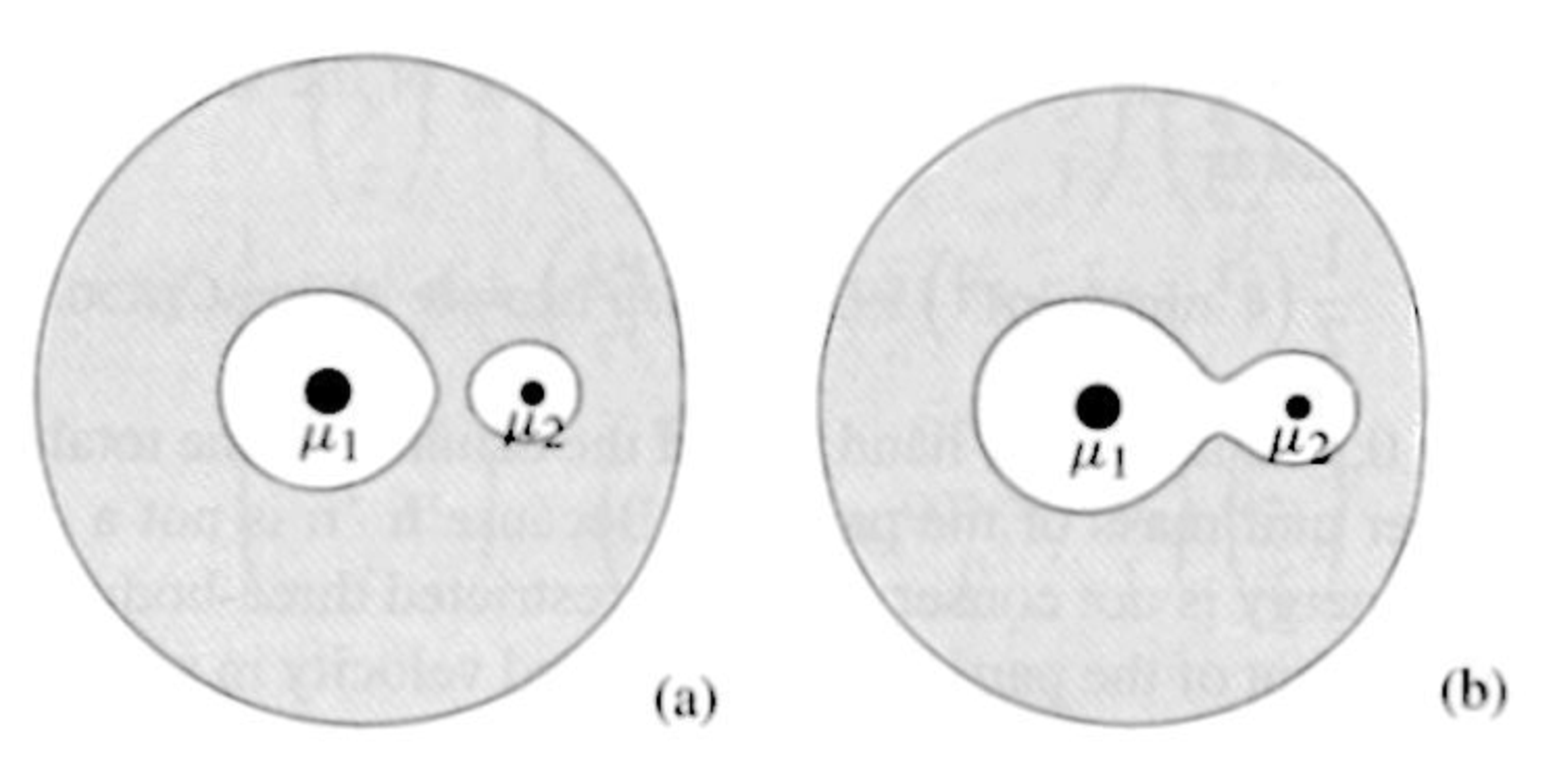
\includegraphics[width=10cm]{./image/sec3_2.pdf}
\caption{$\mu_2 = 0.2$ の場合の2種類のヤコビ積分の値におけるゼロ速度曲線.(Solar System Dynamics\cite{SSD} より引用)\label{fig:zerovelo}}
\end{figure}

粒子の速度が0である場所を考えることで,ヤコビ積分の有用さがわかる.この場合,
\begin{equation}
2 U = C_J
\end{equation}
または,
\begin{equation}
n^2 (x^2 + y^2) + 2 \left( \frac{\mu_1}{r_1} + \frac{\mu_2}{r_2} \right) = C_J \label{eq:zerovelo}
\end{equation}
式(\ref{eq:zerovelo})はある $C_J$ の値の曲面を定義している.この曲面はゼロ速度曲面として知られているもので,粒子の運動に制約を与える上で重要な役割を果たす.簡単のため $x-y$ 平面を考えると,ゼロ速度曲面と $x-y$ 平面が交わるところでは,ゼロ速度曲線を形成する.図\ref{fig:zerovelo}は $\mu_2 = 0.2, n = 1$ の場合のゼロ速度曲線を示している.式(\ref{eq:2U-C_J})から,常に $2 U \geqq C_J$ であることは明らかである.ゆえに式(\ref{eq:zerovelo})は,粒子が運動が不可能な領域の境界線を決定する.したがって,制限3体問題は積分不可能である (任意の初期状態から粒子の運動を解くことができない) が,ヤコビ積分が存在することによって,粒子が存在できない $x-y$ 平面の領域を見つけることができる.この結果は簡単に3次元に拡張できる.

\subsection{ティスランの関係式}
軌道長半径 $a$,離心率 $e$,軌道傾斜角 $I$ をもつ彗星を考える.また,この彗星が木星に接近した後の軌道要素を $a', e', I'$ とする.これらの2組の軌道要素は,ヤコビ積分やいくつかの近似を用いることで簡単に関連づけることができる.ヤコビ積分の値 $C_J = 2 U - v^2$ は接近の間定数である.3次元慣性座標系では,彗星は位置ベクトル ${\bm r} = (\xi, \eta, \zeta)$,速度ベクトル $\dot{{\bm r}} = (\dot{\xi}, \dot{\eta}, \dot{\zeta})$ を持つ.この座標系では,式(\ref{eq:C_J})よりヤコビ積分を以下のように書くことができる.
\begin{equation}
C_J = 2 \left( \frac{\mu_1}{r_1} + \frac{\mu_2}{r_2} \right) + 2 n (\dot{\xi} \eta - \dot{\eta} \xi) - \dot{\xi}^2 - \dot{\eta}^2 - \dot{\zeta}^2 \label{eq:C_Jcomet}
\end{equation}
ここで $r_1, r_2$ はそれぞれ彗星の太陽からと木星からの距離である.木星の軌道長半径を単位長さ,木星の平均運動を単位角速度として選ぶ.また木星と彗星の質量は太陽に比べ十分に小さいため,
\begin{equation}
G (m_{\rm sun} + m_{\rm comet}) \approx G (m_{\rm sun} + m_{\rm Jupiter}) = 1
\end{equation}
ここで $m_{\rm sun}, m_{\rm comet}, m_{\rm Jupiter}$ はそれぞれ太陽,彗星,木星の質量である.太陽-彗星の2体問題のエネルギー積分は式(\ref{eq:v2new})より,
\begin{equation}
\dot{\xi}^2 + \dot{\eta}^2 + \dot{\zeta}^2 = \frac{2}{r} - \frac{1}{a}
\end{equation}
ここで選んだ単位系では $\mu = 1$ であり,また木星と彗星の質量は太陽に比べ無視できるため,$r_1 \approx r$ と仮定した.彗星の単位質量あたりの角運動量は,
\begin{equation}
{\bm h} = {\bm r} \times \dot{{\bm r}}
\end{equation}
木星の軌道面に対する彗星の軌道傾斜角を $I$ とすると,角運動量の $\zeta$ 成分は,
\begin{equation}
\xi \dot{\eta} - \eta \dot{\xi} = h \cos I
\end{equation}
ここで選んだ単位系では $h^2 = a (1 - e^2)$ である.したがって,式(\ref{eq:C_Jcomet})のヤコビ積分の表式から,
\begin{equation}
\frac{2}{r} - \frac{1}{a} - 2 \sqrt{a (1 - e^2)} \cos I = \frac{2}{r} - 2 \mu_2 \left( \frac{1}{r} - \frac{1}{r_2} \right) - C_J
\end{equation}
彗星が木星から遠く $1/r_2$ が常に微少量だとし,$\mu_2$ の項を無視すると,
\begin{equation}
\frac{1}{2a} + \sqrt{a (1 - e^2)} \cos I \approx {\rm const.}
\end{equation}
したがって,彗星の木星接近前後の軌道要素の関係は,近似的に以下のように書くことができる.
\begin{equation}
\frac{1}{2a} + \sqrt{a (1 - e^2)} \cos I = \frac{1}{2a'} + \sqrt{a' (1 - e'^2)} \cos I'
\end{equation}
これはティスランの関係式 (Tisserand relation (Tisserand 1896)) として知られ,新しく発見された彗星が,すでに発見されていた,惑星に接近して軌道要素を変えられた彗星かどうかを判定するのに使うことができる.

\section{摂動関数 \label{sec:disturb_func}}
\ref{sec:3body}節では,制限問題における惑星の位置から3体問題を扱った.しかし,任意の初期条件で2つの物体から重力の影響を受ける,3体目の物体の運動のより一般的な問題に取り組もうとはしなかった.この問題は積分不可能であるが,3体目の物体が受ける加速度を解析することで議論を進めることができる.運動が中心星または主星に支配されているなら,伴星らの軌道は,相互重力摂動によって円錐曲線から少しずれたものとなる.この章では,摂動関数 (disturbing function) の定義と解析によって,このずれがどのように計算できるのかを示す.

質量 $m_c$ の主星のまわりを質量 $m_i$ の天体が楕円軌道で回っている場合を考える.\ref{sec:2body}節でみてきたように,この2体問題は積分可能であり,主星の重力効果が質点によるものみなすと,$m_i$ の天体の軌道要素 $a_i, e_i, I_i, \varpi_i, \Omega_i$ は定数である.ここで3体目の天体 $m_j$ を導入すると,$m_c$ との2体問題での加速度に加えて,$m_i$ と $m_j$ 間の相互重力が加速度に足される (図\ref{fig:disturbingfunc}).主星に対する伴星らの相対的な追加の加速度は,摂動関数と呼ばれる摂動のポテンシャルの勾配から得られる.

この章は,摂動関数のフーリエ級数展開の性質の数学的な解析と関係している.摂動関数の展開式から適切な項を取り出し,その他の項の運動方程式への時間平均された寄与が無視できると仮定し,太陽系力学における特定の問題に取り組む方法を示す.摂動関数の性質を理解することは,太陽系における共鳴の力学やその他の長周期運動を理解する鍵となる.

\begin{figure}[H]
\centering
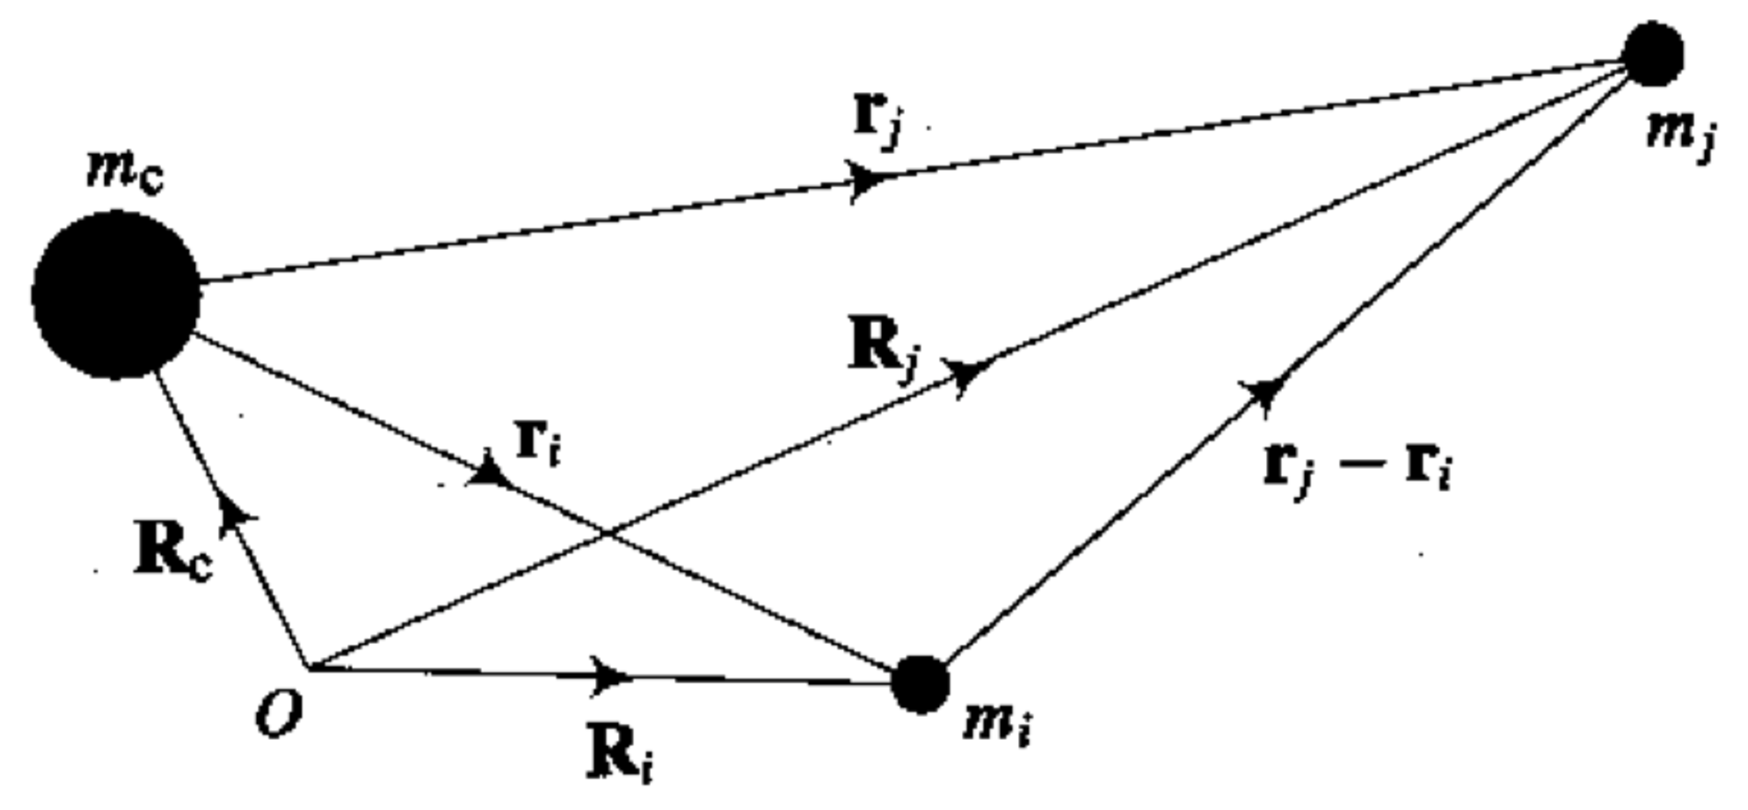
\includegraphics[width=10cm]{./image/sec6_1.pdf}
\caption{主星 $m_c$ に対する2つの伴星 $m_i, m_j$ の相対位置ベクトル ${\bm r}_i, {\bm r}_j$.3つの天体は任意の固定された原点 $O$ からの位置ベクトル ${\bm R}_i, {\bm R}_j, {\bm R}_c$ をもつ.(Solar System Dynamics\cite{SSD} より引用)\label{fig:disturbingfunc}}
\end{figure}

\subsection{摂動関数}
質量 $m_c, m_i, m_j$ の3つの天体の,固定された原点 $O$ に対する位置ベクトルをそれぞれ ${\bm R}_c, {\bm R}_i, {\bm R}_j$ とする.主星 $m_c$ に対する伴星 $m_i, m_j$ の位置ベクトルをそれぞれ ${\bm r}_i, {\bm r}_j$ とすると,
\begin{equation}
|{\bm r}_i| = r_i = (x_i^2 + y_i^2 + z_i^2)^{1/2}, \quad |{\bm r}_j| = r_j = (x_j^2 + y_j^2 + z_j^2)^{1/2},
\end{equation}
そして
\begin{equation}
|{\bm r}_j- {\bm r}_i| = \left[ (x_j - x_i)^2 + (y_j - y_i)^2 + (z_j - z_i)^2 \right]^{1/2}.
\end{equation}
この座標系の原点は主星である (図\ref{fig:disturbingfunc}).

ニュートンの運動の法則と重力の法則より,慣性系における3つの天体の運動方程式が得られる.
\begin{eqnarray}
m_c \ddot{\bm R}_c & = & G m_c m_i \frac{{\bm r}_i}{r_i^3} + G m_c m_j \frac{{\bm r}_j}{r_j^3}, \label{eq:R_c}\\
m_i \ddot{\bm R}_i & = & G m_i m_j \frac{({\bm r}_j - {\bm r}_i)}{|{\bm r}_j - {\bm r}_i|^3} - G m_i m_c \frac{{\bm r}_i}{r_i^3}, \label{eq:R_i}\\
m_j \ddot{\bm R}_j & = & G m_j m_i \frac{({\bm r}_i - {\bm r}_j)}{|{\bm r}_i - {\bm r}_j|^3} - G m_j m_c \frac{{\bm r}_j}{r_j^3}. \label{eq:R_j}
\end{eqnarray}
主星に対する伴星の加速度は次のように与えられる.
\begin{eqnarray}
\ddot{\bm r}_i & = & \ddot{\bm R}_i - \ddot{\bm R}_c, \\
\ddot{\bm r}_j & = & \ddot{\bm R}_j - \ddot{\bm R}_c.
\end{eqnarray}
式(\ref{eq:R_c}),式(\ref{eq:R_i}),式(\ref{eq:R_j})から $\ddot{\bm R}_c, \ddot{\bm R}_i, \ddot{\bm R}_j$ の表式を代入すると,
\begin{eqnarray}
\ddot{\bm r}_i + G (m_c + m_i) \frac{{\bm r}_i}{r_i^3} & = & G m_j \left( \frac{{\bm r}_j - {\bm r}_i}{| {\bm r}_j - {\bm r}_i |^3} - \frac{{\bm r}_j}{r_j^3} \right), \label{eq:r_i} \\ 
\ddot{\bm r}_j + G (m_c + m_j) \frac{{\bm r}_j}{r_j^3} & = & G m_i \left( \frac{{\bm r}_i - {\bm r}_j}{| {\bm r}_i - {\bm r}_j |^3} - \frac{{\bm r}_i}{r_i^3} \right). \label{eq:r_j}
\end{eqnarray}
これらの相対加速度は,スカラー関数の勾配として次のように書ける.
\begin{eqnarray}
\ddot{\bm r}_i & = & \nabla_i (U_i + {\cal R}_i) = \left( \hat{\bf i} \frac{\partial}{\partial x_i} + \hat{{\bf j}} \frac{\partial}{\partial y_i} + \hat{\bf k} \frac{\partial}{\partial z_i} \right) (U_i + {\cal R}_i), \label{eq:r_i_nabla} \\ 
\ddot{\bm r}_j & = & \nabla_j (U_j + {\cal R}_j) = \left( \hat{\bf i} \frac{\partial}{\partial x_j} + \hat{{\bf j}} \frac{\partial}{\partial y_j} + \hat{\bf k} \frac{\partial}{\partial z_j} \right) (U_j + {\cal R}_j), \label{eq:r_j_nabla}
\end{eqnarray}
ここで,
\begin{equation}
U_i = G \frac{m_c + m_i}{r_i} \quad {\rm and} \quad U_j = G \frac{m_c + m_j}{r_j}
\end{equation}
は全体のポテンシャルのうちの2体問題の部分である.$\nabla$ 演算子の添字 $i, j$ は,勾配を $m_i, m_j$ それぞれの座標についてとることを強調している.ポテンシャル中の${\cal R}$ の項は摂動関数であり,他の伴星によって生じるポテンシャルを表している.${\bm r}_i$ は $x_j, y_j, z_j$ によらず,${\bm r}_j$ は $x_i, y_i, z_i$ によらないので,次のように書ける.
\begin{eqnarray}
{\cal R}_i & = & \frac{G m_j}{ |{\bm r}_j - {\bm r}_i| } - G m_j \frac{ {\bm r}_i \cdot {\bm r}_j }{r_j^3}, \\
{\cal R}_j & = & \frac{G m_i}{ |{\bm r}_i - {\bm r}_j| } - G m_i \frac{ {\bm r}_i \cdot {\bm r}_j }{r_i^3}.
\end{eqnarray}
第一項は直接項 (direct terms) と呼ばれ,座標系の原点のとり方によって生じる第二項は間接項 (indirect terms) と呼ばれる.座標系の原点が重心にある場合,この間接項は現れない.

上記の解析は天体の数を増やしても拡張できる.さらに,摂動関数に関係した加速度は,質点の重力に限らずどのような原因からでも生じうる.例えば,主星の扁平性によるポテンシャルから生じる.ここから先,この章では,質量がそれぞれ $m, m'$ で主星に対する位置ベクトルがそれぞれ ${\bm r}, {\bm r'}$ である2つの伴星を質点とみなす特別な場合を主に考える.ここで常に $r < r'$ とする.このとき,内側の伴星の運動方程式は,
\begin{equation}
\ddot{\bm r} + G (m_c + m) \frac{{\bm r}}{r^3} = G m' \left( \frac{{\bm r'} - {\bm r}}{| {\bm r'} - {\bm r} |^3} - \frac{{\bm r'}}{r'^3} \right)
\end{equation}
そして内側の伴星の摂動関数は,
\begin{equation}
{\cal R} = \frac{\mu'}{ |{\bm r'} - {\bm r}| } - \mu' \frac{ {\bm r} \cdot {\bm r'} }{r'^3} \label{eq:cal_R1}
\end{equation}
ここで $\mu' = G m'$ であり,内側の伴星の基準軌道は接触軌道要素 $n^2 a^3 = G (m_c + m)$ を持つ.同様に外側の伴星に関する運動方程式は,
\begin{equation}
\ddot{\bm r'} + G (m_c + m') \frac{{\bm r'}}{r'^3} = G m \left( \frac{{\bm r} - {\bm r'}}{| {\bm r} - {\bm r'} |^3} - \frac{{\bm r}}{r^3} \right)
\end{equation}
そして外側の伴星の摂動関数は,
\begin{equation}
{\cal R'} = \frac{\mu}{ |{\bm r} - {\bm r'}| } - \mu \frac{ {\bm r} \cdot {\bm r'} }{r^3} \label{eq:cal_R'1}
\end{equation}
ここで $\mu = G m$ であり,外側の伴星の基準軌道は接触軌道要素 $n'^2 a'^3 = G (m_c + m')$ を持つ.

以上は ${\cal R}, {\cal R'}$ の最も素直な求め方であるが,この求め方や結果の表式は唯一のものではない.例えば,${\cal R'}$ の式の両辺に $- \frac{\mu}{r'}$ の項を加えると,$m'$ の運動方程式の両辺に $G m \frac{{\bm r'}}{r'^3}$ の項を加えることが可能である.ただし,このとき,$m'$ の基準軌道は接触軌道要素 $n'^2 a'^3 = G (m_c + m + m')$ を持つ.

\subsection{ルジャンドル多項式を用いた展開}
\begin{figure}[H]
\centering
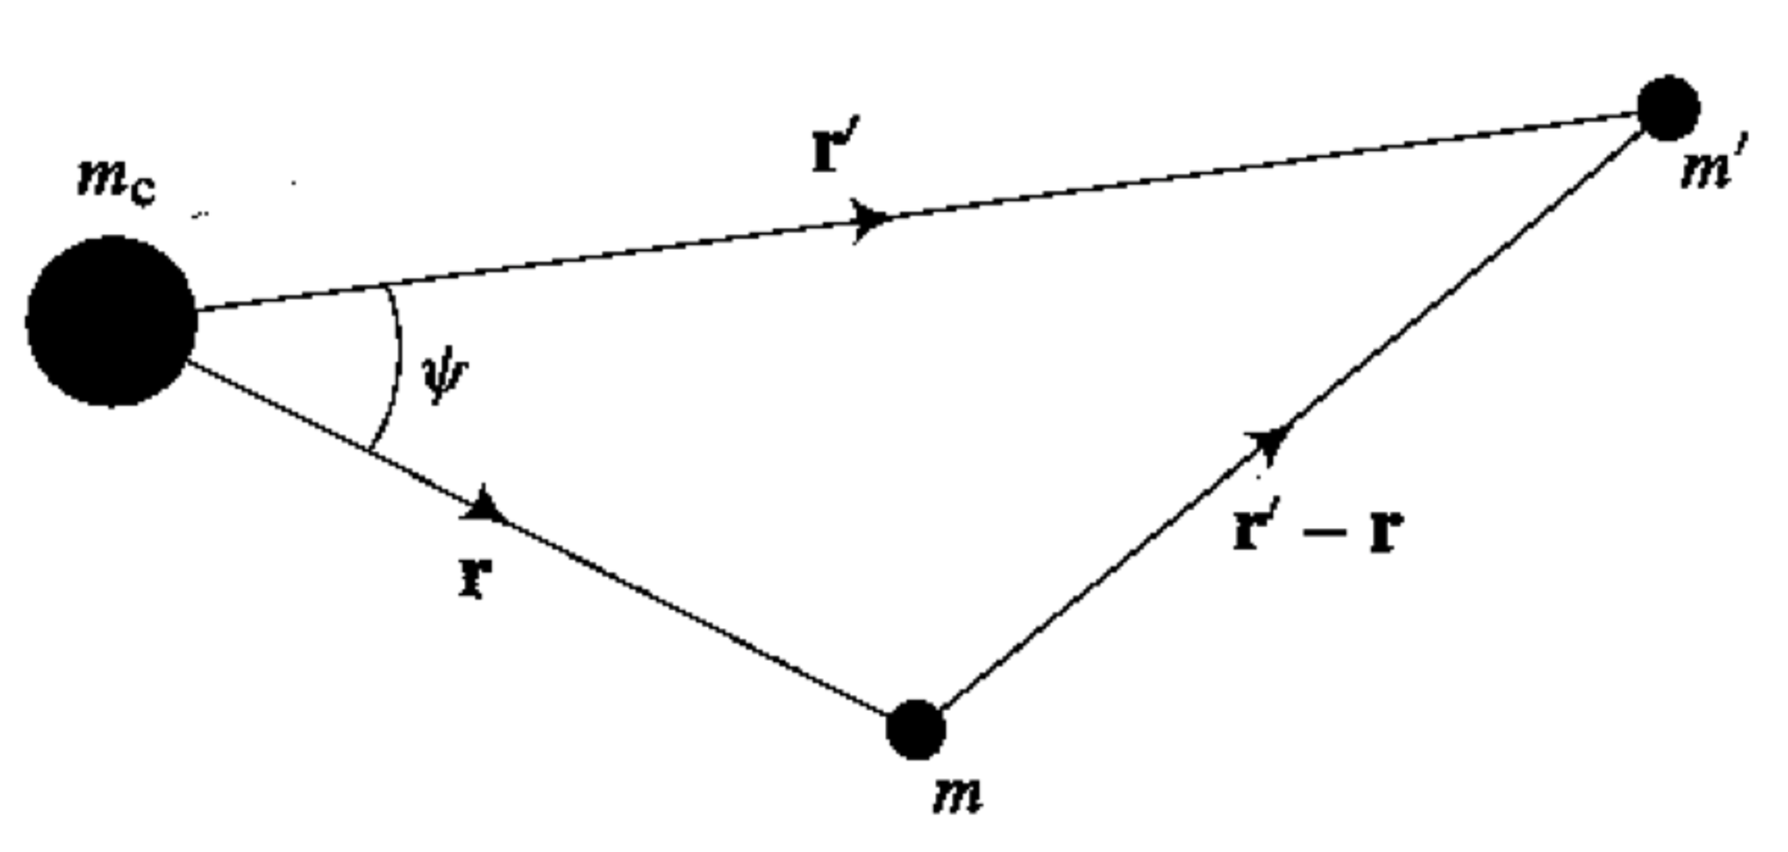
\includegraphics[width=10cm]{./image/sec6_2.pdf}
\caption{主星 $m_c$ に対する2つの伴星 $m, m'$ の位置ベクトル ${\bm r}, {\bm r}'$.位置ベクトルのなす角は $\psi$.(Solar System Dynamics\cite{SSD} より引用)\label{fig:disturbingfunc_psi}}
\end{figure}
図\ref{fig:disturbingfunc_psi}に示すような,質量がそれぞれ $m, m'$ で主星に対する位置ベクトルがそれぞれ ${\bm r}, {\bm r'}$ である2つの伴星を考える.この2つの位置ベクトルのなす角を $\psi$ とする.余弦定理より,
\begin{equation}
|{\bm r'} - {\bm r}|^2 = r^2 + r'^2 - 2 r r' \cos \psi,
\end{equation}
または,
\begin{equation}
\frac{1}{|{\bm r'} - {\bm r}|} = \frac{1}{r'} \left[ 1 - 2 \frac{r}{r'} \cos \psi + \left( \frac{r}{r'} \right)^2 \right]^{-\frac{1}{2}}
\end{equation}
これはルジャンドル多項式で展開でき,
\begin{equation}
\frac{1}{|{\bm r'} - {\bm r}|} = \frac{1}{r'} \sum_{l = 0}^{\infty} \left( \frac{r}{r'} \right)^l P_l (\cos \psi)
\end{equation}
ここで $P_0 (\cos \psi) = 1, P_1 (\cos \psi) = \cos \psi, P_2 (\cos \psi) = \frac{1}{2} (3 \cos^2 \psi - 1), \cdots$ である.${\bm r} \cdot {\bm r'} = r r' \cos \psi = r r' P_1 (\cos \psi)$ なので,内側の伴星の摂動関数は,
\begin{equation}
{\cal R} = \frac{\mu'}{r'} \sum_{l = 2}^{\infty} \left( \frac{r}{r'} \right)^l P_l (\cos \psi) \label{eq:cal_R2}
\end{equation}
ここで,$P_0 (\cos \psi)$ の項は $r$ に依存せず,内側の伴星の座標に対する ${\cal R}$ の勾配のみに興味があるため,この式からは省略している.同様に,外側の伴星の摂動関数は,
\begin{equation}
{\cal R'} = \frac{\mu}{r'} \sum_{l = 2}^{\infty} \left( \frac{r}{r'} \right)^l P_l (\cos \psi) + \mu \frac{r}{r'^2} \cos \psi - \mu \frac{r'}{r^2} \cos \psi
\end{equation}
したがって,後ろの二項 (ここで扱う利用法において実質的に重要でない) を別として,${\cal R}, {\cal R'}$ の表式はとても似ている.

この章では摂動関数 ${\cal R}, {\cal R'}$ の,$m, m'$ の軌道要素 (直交座標ではなく) についての級数展開を扱う.ここで,標準軌道要素 $a, e, I, \varpi, \Omega, \lambda$ を用い,それぞれ $m$ の軌道長半径,離心率,軌道傾斜角,近日点経度,昇交点経度,平均経度 ($\lambda = M + \varpi$) を意味する.$m'$ についてはプライムをつけて表す.${\cal R}$ の展開式は,
\begin{equation}
{\cal R} = \mu' \sum S (a,a',e,e',I,I') \cos \varphi \label{eq:cal_R_varphi}
\end{equation}
の形で表される.ここで $\varphi$ は,
\begin{equation}
\varphi = j_1 \lambda' + j_2 \lambda + j_3 \varpi' + j_4 \varpi + j_5 \Omega' + j_6 \Omega \label{eq:varphi}
\end{equation}
という線形結合の形で表され,$j_i (i = 1,2,…,6)$ は整数であり,
\begin{equation}
\sum_{i = 1}^{6} j_i = 0
\end{equation}
である.これはダランベールの関係式 (d'Alembert relation) という.この性質は主星のポテンシャルが方位角に対して不変であることに由来する.角変数に何をつかってもよいわけではなく,固定された方向からの角度 (すなわち,離角ではなく経度) を用いなければならない.関数 $S$ の詳細な形と $\varphi$ における許容される角の組み合わせを知ることにより,運動方程式に対して支配的な寄与をする項や,逆に無視できる項を見分けることができる.

式(\ref{eq:cal_R2})の動径方向に依存する部分に注目すると,
\begin{equation}
{\cal R} = \frac{\mu}{a'} \sum_{l = 2}^{\infty} \alpha^l \left( \frac{a'}{r'} \right)^{l+1} \left( \frac{r}{a} \right)^l P_l (\cos \psi)
\end{equation}
ここで,
\begin{equation}
\alpha = \frac{a}{a'} < 1
\end{equation}
は $m$ と $m'$ の軌道長半径の比である.

摂動関数の展開はよくコンピュータの助けを借りて行われる作業である.最終的に得られる結果は膨大な数の偏角からなる $\alpha$ の級数である.

摂動関数 ${\cal R}$ はKaula (1961, 1962) によって開発された手法により,標準軌道要素で展開できる.この手法では,摂動関数は主星の赤道を基準とした接触楕円要素で無限級数展開される.
\begin{equation}
\begin{split}
{\cal R} = & \frac{\mu'}{a'} \sum_{l = 2}^{\infty} \alpha^l \sum_{m = 0}^l (-1)^{l - m} \kappa_m \frac{(l - m) !}{(l + m) !} \\
& \times \sum_{p,p' = 0}^l F_{lmp} (I) F_{lmp'} (I') \sum_{q,q' = - \infty}^{\infty} X_{l - 2p + q}^{l, l - 2p} (e) X_{l - 2p' + q'}^{-l -1, l - 2p'} (e') \\
& \times \cos [ (l - 2p' + q') \lambda' - (l - 2p + q) \lambda - q' \varpi' + q \varpi \\
& \quad \quad \quad+ (m - l + 2p') \Omega' - (m - l + 2p) \Omega ]
\end{split}
\end{equation}
ここで $\alpha = a / a'$ であり,$\lambda, \lambda'$ は平均経度,$\varpi, \varpi'$ は近日点経度である.また,$\kappa_0 = 1, \kappa_m = 2 \ {\rm for} \ m \not = 0$ である.

関数 $F_{lmp} (I)$ は軌道傾斜角関数であり,次のように定義される.
\begin{equation}
\begin{split}
F_{lmp} (I) = & \frac{{\rm i}^{l - m} (l + m) !}{2^l p ! (l - m) !} \\
& \times \sum_k (-1)^k 
\begin{pmatrix}
2l - 2p \\
k \\
\end{pmatrix}
\begin{pmatrix}
2p \\
l - m - k \\
\end{pmatrix}
c^{3l - m - 2p - 2k} s^{m - l + 2p + 2k}
\end{split} \label{eq:F_lmp}
\end{equation}
ここで ${\rm i} = \sqrt{-1}$ であり,$k$ については $k = {\rm max} (0, l - m - 2p)$ から $k = {\rm min} (l - m, 2l - 2p)$ まで和をとる.また,$s \equiv \sin \frac{1}{2} I, c \equiv \cos \frac{1}{2} I$ とした.

$X_c^{a, b} (e)$ はハンセン係数 (Hansen coefficients) であり,次のように定義できる.
\begin{equation}
X_c^{a, b} (e) = e^{|c - b|} \sum_{\sigma = 0}^{\infty} X_{\sigma + \alpha, \sigma + \beta}^{a, b} e^{2 \sigma}
\end{equation}
ここで,$\alpha = {\rm max} (0, c - b), \beta = {\rm max} (0, b - c)$ である.また $X_{c, d}^{a, b}$ はニューカム演算子 (Newcomb operators) であり,次のように再帰的に定義される.
\begin{eqnarray}
X_{0, 0}^{a, b} = 1,\\
X_{1, 0}^{a, b} = b - a / 2,
\end{eqnarray}
$d = 0$ のとき,
\begin{equation}
4 c X_{c, 0}^{a, b} = 2 (2b - a) X_{c - 1, 0}^{a, b + 1} + (b - a) X_{c - 2, 0}^{a, b + 2},
\end{equation}
$d \not = 0$ のとき,
\begin{equation}
\begin{split}
4 c X_{c, d}^{a, b} = & -2 (2b + a) X_{c, d - 1}^{a, b - 1} - (b + a) X_{c, d - 2}^{a, b - 2} \\
& - (c - 5d + 4 + 4b +a) X_{c - 1, d - 1}^{a, b} \\
& + 2 (c - d + b) \sum_{j \geqq 2} (-1)^j
\begin{pmatrix}
3/2 \\
j \\
\end{pmatrix}
X_{c - j, d - j}^{a, b}.
\end{split} \label{eq:4dX}
\end{equation}
また,$c < 0$ または $d < 0$ のとき $X_{c, d}^{a, b} = 0$,$d > c$ のとき $X_{c, d}^{a, b} = X_{d, c}^{a, -b}$ である.

Plummer (1918) とHughes (1981) にはハンセン係数とニューカム演算子に関する詳細な記述がある.特にHughes (1981) にはハンセン係数の性質や様々な再帰関係について述べている.

${\cal R'}$ の展開も考えると,
\begin{equation}
\begin{split}
{\cal R'} = & \frac{\mu}{a'} \sum_{l = 1}^{\infty} \alpha^l \sum_{m = 0}^l \kappa_m \frac{(l - m) !}{(l + m) !} \\
& \times \sum_{p,p' = 0}^l F_{lmp} (I) F_{lmp'} (I') \sum_{q,q' = - \infty}^{\infty} X_{l - 2p + q}^{l, l - 2p} (e) X_{l - 2p' + q'}^{-l -1, l - 2p'} (e') \\
& \times \cos [ (l - 2p' + q') \lambda' - (l - 2p + q) \lambda - q' \varpi' + q \varpi \\
& \quad \quad \quad + (m - l + 2p') \Omega' - (m - l + 2p) \Omega ] \\
& - \frac{\mu a'}{a^2} \sum_{m = 0}^1 \kappa_m \frac{(1 - m) !}{(1 + m) !} \\
& \times \sum_{p,p' = 0}^1 F_{1mp} (I) F_{1mp'} (I') \sum_{q,q' = - \infty}^{\infty} X_{1 - 2p + q}^{-2, 1 - 2p} (e) X_{1 - 2p' + q'}^{1, 1 - 2p'} (e') \\
& \times \cos [ (1 - 2p' +q') \lambda' - (1 -2p + q) \lambda - q' \varpi' +q \varpi \\
& \quad \quad \quad + (m - 1 + 2p') \Omega' - (m - 1 + 2p) \Omega ].
\end{split}
\end{equation}

展開の複雑さを考えると,摂動関数の直接部と間接部を区別することが慣習的に行われる.式(\ref{eq:cal_R1}),式(\ref{eq:cal_R'1})の定義より,次のように書ける.
\begin{eqnarray}
{\cal R} & = & \frac{\mu'}{a'} {\cal R}_{\rm D} + \frac{\mu'}{a'} \alpha {\cal R}_{\rm E} \label{eq:cal_R3} \\
{\cal R'} & = & \frac{\mu}{a'} {\cal R}_{\rm D} + \frac{\mu}{a'} \frac{1}{\alpha^2} {\cal R}_{\rm I} \label{eq:cal_R'3}
\end{eqnarray}
ここで,
\begin{eqnarray}
{\cal R}_{\rm D} & = & \frac{a'}{|{\bm r'} - {\bm r}|}, \label{eq:cal_RD}\\
{\cal R}_{\rm E} & = & - \left( \frac{r}{a} \right) \left( \frac{a'}{r'} \right)^2 \cos \psi, \label{eq:cal_RE} \\
{\cal R}_{\rm I} & = & - \left( \frac{r'}{a'} \right) \left( \frac{a}{r} \right)^2 \cos \psi. \label{eq:cal_RI}
\end{eqnarray}
${\cal R}_{\rm D}$ は直接部,${\cal R}_{\rm E}$ は外側の摂動源による間接部,${\cal R}_{\rm I}$ は内側の摂動源による間接部から得られるものである.式(\ref{eq:cal_R3}),式(\ref{eq:cal_R'3}),式(\ref{eq:cal_RD})から明らかなように,${\cal R}_{\rm D}$ の表式を用いて ${\cal R}, {\cal R'}$ の直接部を得ることができる.

式(\ref{eq:cal_R_varphi}),式(\ref{eq:varphi})から,これらは角変数 $\varphi$ のオーダー,すなわち $\lambda$ と $\lambda'$ の係数の和によって分類できる.

直接部の二次のオーダーまでの展開式は,${\cal R}^{(i)}$ がオーダー $i$ の角変数を含む部分を表すとすると,
\begin{equation}
{\cal R}_{\rm D} =  {\cal R}_{\rm D}^{(0)} + {\cal R}_{\rm D}^{(1)} + {\cal R}_{\rm D}^{(2)} \label{eq:cal_RD(012)}
\end{equation}
\begin{equation}
\begin{split}
{\cal R}_{\rm D}^{(0)} = & \left( \frac{1}{2} b_{ \frac{1}{2} }^{(j)} + \frac{1}{8} (e^2 + e'^2) [ -4 j^2 + 2 \alpha D + \alpha^2 D^2 ] b_{ \frac{1}{2} }^{(j)} \right. \\
& \left. \quad + \frac{1}{4} (s^2 + s'^2) \left( [- \alpha ] b_{ \frac{3}{2} }^{(j - 1)} + [- \alpha ] b_{ \frac{3}{2} }^{(j + 1)} \right) \right) \\
& \quad \times \cos [j \lambda' - j \lambda ] \\
& + \left( \frac{1}{4} e e' [ 2 + 6j + 4 j^2 - 2 \alpha D - \alpha^2 D^2] b_{ \frac{1}{2} }^{(j + 1)} \right) \\
& \quad \times \cos [j \lambda' - j \lambda + \varpi' - \varpi ] \\
& + \left( s s' [ \alpha ] b_{ \frac{3}{2} }^{(j + 1)} \right) \cos [ j \lambda' - j \lambda + \Omega' - \Omega ]
\end{split} \label{eq:cal_RD(0)}
\end{equation}
\begin{equation}
\begin{split}
{\cal R}_{\rm D}^{(1)} = & \left( \frac{1}{2} e [-2 j - \alpha D] b_{ \frac{1}{2} }^{(j)} \right) \cos [j \lambda' + (1 -j) \lambda - \varpi ] \\
& + \left( \frac{1}{2} e' [ -1 + 2 j + \alpha D] b_{ \frac{1}{2} }^{(j - 1)} \right) \cos [j \lambda' + (1 -j) \lambda - \varpi' ]
\end{split}  \label{eq:cal_RD(1)}
\end{equation}
\begin{equation}
\begin{split}
{\cal R}_{\rm D}^{(2)} = & \left( \frac{1}{8} e^2 [-5 j + 4 j^2 - 2 \alpha D + 4 j \alpha D + \alpha^2 D^2] b_{ \frac{1}{2} }^{(j)} \right) \\
& \quad \times \cos [j \lambda' + (2 - j) \lambda - 2 \varpi ] \\
& + \left( \frac{1}{4} e e' [ -2 + 6 j - 4 j^2 + 2 \alpha D - 4 j \alpha D - \alpha^2 D^2] b_{ \frac{1}{2} }^{(j - 1)} \right) \\
& \quad \times \cos [j \lambda' + (2 -j) \lambda - \varpi' - \varpi ] \\
& + \left( \frac{1}{8} e'^2 [2 -7 j + 4 j^2 - 2 \alpha D + 4 j \alpha D + \alpha^2 D^2] b_{ \frac{1}{2} }^{(j - 2)} \right) \\
& \quad \times \cos [j \lambda' + (2 - j) \lambda - 2 \varpi' ] \\
& + \left( \frac{1}{2} s^2 [ \alpha ] b_{ \frac{3}{2} }^{(j - 1)} \right) \cos [j \lambda' + (2 - j) \lambda - 2 \Omega ] \\
& + \left( s s' [ - \alpha ] b_{ \frac{3}{2} }^{(j - 1)} \right) \cos [j \lambda' + (2 - j) \lambda - \Omega' - \Omega] \\
& + \left( \frac{1}{2} s'^2 [ \alpha ] b_{ \frac{3}{2} }^{(j - 1)} \right) \cos [j \lambda' + (2 - j) \lambda - 2 \Omega' ]
\end{split} \label{eq:cal_RD(2)}
\end{equation}
ここで,$s \equiv \sin \frac{I}{2}$,$\alpha = a/a'$.$D \equiv d/d \alpha$ は微分演算子.また,$b_{i + \frac{1}{2}}^{(j)}(\alpha)$ はラプラス係数 (Laplace coefficients) であり,$i$ を整数として,
\begin{equation}
\frac{1}{2} b_{i + \frac{1}{2}}^{(j)} = \frac{1}{2 \pi} \int_0^{2 \pi} \frac{\cos j \psi d \psi}{(1 - 2 \alpha \cos \psi + \alpha^2)^{i + \frac{1}{2}}}
\end{equation}
と定義される.

式(\ref{eq:cal_RE}),式(\ref{eq:cal_RI})で定義された間接部の展開式は,離心率と軌道傾斜角を微少量だとして楕円展開 (elliptical expansion) を使うと比較的簡単に求めることができる.$\cos \psi, (r/a), (a'/r')$ の $e, I$ の二次までの展開は,
\begin{equation}
\begin{split}
\cos \psi \approx & (1 - e^2 - e'^2 - s^2 - s'^2) \cos [\lambda - \lambda'] \\
& + e e' \cos [2 \lambda - 2 \lambda' - \varpi - \varpi'] \\
& + e e' \cos [\varpi - \varpi'] + 2 s s' \cos [\lambda - \lambda' - \Omega + \Omega'] \\
& + e \cos [2 \lambda - \lambda' - \varpi] - e \cos [\lambda' - \varpi] \\
& + e' \cos [\lambda - 2 \lambda' + \varpi'] - e' \cos [\lambda - \varpi'] \\
& + \frac{9}{8} e^2 \cos [3 \lambda - \lambda' - 2 \varpi] - \frac{1}{8} e^2 \cos [\lambda + \lambda' - 2 \varpi] \\
& + \frac{9}{8} e'^2 \cos [\lambda - 3 \lambda' + 2 \varpi'] - \frac{1}{8} e'^2 \cos [\lambda + \lambda' - 2 \varpi'] \\
& - e e' \cos [2 \lambda - \varpi - \varpi'] - e e' \cos [2 \lambda' - \varpi - \varpi'] \\
& + s^2 \cos [\lambda + \lambda' - 2 \Omega] + s'^2 \cos [\lambda + \lambda' - 2 \Omega'] \\
& - 2 s s' \cos [\lambda + \lambda' - \Omega - \Omega']
\end{split}
\end{equation}
\begin{eqnarray}
\left( \frac{r}{a} \right) & = & 1 - e \cos [\lambda - \varpi] + \frac{1}{2} e^2 \left(1 - \cos [2 \lambda - 2 \varpi] \right) \\
\left( \frac{a'}{r'} \right) & = & 1 + 2 e' \cos [\lambda' - \varpi'] + \frac{1}{2} e'^2 \left(1 + 5 \cos [2 \lambda' - 2 \varpi'] \right)
\end{eqnarray}

したがって,${\cal R}_{\rm E}$ の $e, I$ の二次までの展開は,
\begin{equation}
\begin{split}
{\cal R}_{\rm E} = & - \left( \frac{r}{a} \right) \left( \frac{a'}{r'} \right)^2 \cos \psi \\
\approx & \left( -1 + \frac{1}{2} e^2 + \frac{1}{2} e'^2 + s^2 + s'^2 \right) \cos [\lambda' - \lambda] \\
& - e e' \cos [2 \lambda' - 2 \lambda - \varpi' + \varpi] - 2 s s' \cos [\lambda' - \lambda - \Omega' + \Omega] \\
& - \frac{1}{2} e \cos [\lambda' -2 \lambda + \varpi] + \frac{3}{2} e \cos [\lambda' - \varpi] - 2 e' \cos [2 \lambda' - \lambda - \varpi'] \\
& - \frac{3}{8} e^2 \cos [\lambda' - 3 \lambda + 2 \varpi] - \frac{1}{8} e^2 \cos [\lambda' + \lambda - 2 \varpi] \\
& + 3 e e' \cos [2 \lambda - \varpi' - \varpi] - \frac{1}{8} e'^2 \cos [\lambda' + \lambda - 2 \varpi'] \\
& - \frac{27}{8} e'^2 \cos [3 \lambda' - \lambda - 2 \varpi'] - s^2 \cos [\lambda' + \lambda - 2 \Omega] \\
& + 2 s s' \cos [\lambda' + \lambda - \Omega' - \Omega] - s'^2 \cos [\lambda' + \lambda - 2 \Omega']
\end{split} \label{eq:cal_RE(012)}
\end{equation}
ただし,${\cal R}_{\rm D}$ を求めたときと同じ形にするため,偏角の符号を変えている.

${\cal R}_{\rm I}$ の $e, I$ の二次までの展開は,${\cal R}_{\rm E}$ の表式の中のプライム付きの量とプライムなしの量を入れ替えればよい.
\begin{equation}
\begin{split}
{\cal R}_{\rm I} = & - \left( \frac{r'}{a'} \right) \left( \frac{a}{r} \right)^2 \cos \psi \\
\approx & \left( -1 + \frac{1}{2} e^2 + \frac{1}{2} e'^2 + s^2 + s'^2 \right) \cos [\lambda' - \lambda] \\
& - e e' \cos [2 \lambda' - 2 \lambda - \varpi' + \varpi] - 2 s s' \cos [\lambda' - \lambda - \Omega' + \Omega] \\
& -2 e \cos [\lambda' -2 \lambda + \varpi] + \frac{3}{2} e' \cos [\lambda - \varpi'] - \frac{1}{2} e' \cos [2 \lambda' - \lambda - \varpi'] \\
& - \frac{27}{8} e^2 \cos [\lambda' - 3 \lambda + 2 \varpi] - \frac{1}{8} e^2 \cos [\lambda' + \lambda - 2 \varpi] \\
& + 3 e e' \cos [2 \lambda - \varpi' - \varpi] - \frac{1}{8} e'^2 \cos [\lambda' + \lambda - 2 \varpi'] \\
& - \frac{3}{8} e'^2 \cos [3 \lambda' - \lambda - 2 \varpi'] - s^2 \cos [\lambda' + \lambda - 2 \Omega] \\
& + 2 s s' \cos [\lambda' + \lambda - \Omega' - \Omega] - s'^2 \cos [\lambda' + \lambda - 2 \Omega']
\end{split}
\end{equation}

\subsection{摂動関数の利用}
ここまでの解析で,$r' > r$ (すなわち,軌道は交差しない) と仮定してきた.級数展開が収束するかどうかは,軌道が交差にどれだけ近いかに依存している.式(\ref{eq:cal_R1}),式(\ref{eq:cal_R'1})より,もし軌道が交差するなら,ある経度では ${\bm r} = {\bm r'}$ となり第一項が定義できなくなるため,明らかに特異点が存在する.したがって収束のおおよその条件は,
\begin{equation}
a (1 + e) < a' (1 - e')
\end{equation}
つまり,内側の軌道の遠日点距離が,外側の軌道の近日点距離よりも短いことである.

次に,式(\ref{eq:cal_R_varphi})より,${\cal R} = \mu' \sum S (a,a',e,e',I,I') \cos \varphi$ の $S$ の形,すなわち各項の「強さ」を考える.$X_{l - 2p + q}^{l, l - 2p} (e)$ と $F_{lmp} (I)$ の性質より,離心率と軌道傾斜角の最低次の項を計算することができる.式(\ref{eq:F_lmp})から式(\ref{eq:4dX})を用いると,
\begin{equation}
X_{l - 2p + q}^{l, l - 2p} (e) = \mathcal{O} (e^{|q|}), \quad X_{l - 2p' + q'}^{-l -1, l - 2p'} (e') = \mathcal{O} (e'^{|q'|})
\end{equation}
\begin{equation}
F_{lmp} (I) = \mathcal{O} (s^{|m - l + 2p|}), \quad F_{lmp'} (I') = \mathcal{O} (s'^{|m - l + 2p'|})
\end{equation}
ここで,$s \equiv \sin \frac{1}{2} I, s' \equiv \sin \frac{1}{2} I'$ である.よって,
\begin{equation}
S \approx \frac{f (\alpha)}{a'} e^{|q|} e'^{|q'|} s^{|m - l + 2p|} s'^{|m - l + 2p'|} = \frac{f (\alpha)}{a'} e^{|j_4|} e'^{|j_3|} s^{|j_6|} s'^{|j_5|} \label{eq:S}
\end{equation}
ここで,$f (\alpha)$ はラプラス係数の関数として表される.したがって例えば $e$ の最低次は,最小でもその項の中の $\varpi$ の係数の絶対値に等しい.同様に,$e', \sin \frac{1}{2} I, \sin \frac{1}{2} I'$ の最低次は $\varpi', \Omega, \Omega'$ の係数の絶対値に等しいかそれ以上である.

\subsection{ラグランジュの惑星方程式}
摂動関数の展開によって,摂動のポテンシャルの軌道要素に対する依存性を明らかにしてきた.ここからは,摂動を受けた天体の軌道変化の量を表すことが必要である.そこで,ラグランジュの惑星方程式 (Lagrange's planetary equations) を用いる.ここでは方程式の説明だけにとどめる.完全な導出は,Brouwer \& Clemence (1961) とRoy (1988) に記されている.

ラグランジュの惑星方程式を使うために,新たな角度を導入する必要がある.
\begin{equation}
\lambda = M + \varpi = n (t - \tau) + \varpi = n t + \epsilon \label{eq:lambda}
\end{equation}
ここで,$\lambda$ は平均経度 (mean longitude),$M$ は平均近点離角 (mean anomaly),$\varpi$ は近日点経度 (longitude of pericentre),$t$ は時間,$\tau$ は近点通過時刻 (time of pericentre passage),そして新たな角度 $\epsilon$ は元期 ($t = 0$) での平均経度 (mean longitude at epoch) である.軌道要素の変化に関するラグランジュの惑星方程式は,
\begin{eqnarray}
\frac{d a}{d t} & = & \frac{2}{n a} \frac{\partial {\cal R}}{\partial \epsilon}, \label{eq:dadt} \\
\frac{d e}{d t} & = & - \frac{\sqrt{1 - e^2}}{n a^2 e} \left( 1 - \sqrt{1 - e^2} \right) \frac{\partial {\cal R}}{\partial \epsilon} - \frac{\sqrt{1 - e^2}}{n a^2 e} \frac{\partial {\cal R}}{\partial \varpi}, \label{eq:dedt} \\
\frac{d \epsilon}{d t} & = & - \frac{2}{n a} \frac{\partial {\cal R}}{\partial a} + \frac{\sqrt{1 - e^2}}{n a^2 e} \left( 1 - \sqrt{1 - e^2} \right) \frac{\partial {\cal R}}{\partial e} + \frac{\tan \frac{1}{2} I}{n a^2 \sqrt{1 - e^2}} \frac{\partial {\cal R}}{\partial I}, \label{eq:depsilondt} \\
\frac{d \Omega}{d t} & = & \frac{1}{n a^2 \sqrt{1 - e^2} \sin I} \frac{\partial {\cal R}}{\partial I}, \label{eq:dOmegadt} \\
\frac{d \varpi}{d t} & = & \frac{\sqrt{1 - e^2}}{n a^2 e} \frac{\partial {\cal R}}{\partial e} + \frac{\tan \frac{1}{2} I}{n a^2 \sqrt{1 - e^2}} \frac{\partial {\cal R}}{\partial I}, \label{eq:dvarpidt} \\
\frac{d I}{d t} & = & - \frac{\tan \frac{1}{2} I}{n a^2 \sqrt{1 - e^2}} \left( \frac{\partial {\cal R}}{\partial \epsilon} + \frac{\partial {\cal R}}{\partial \varpi} \right) - \frac{1}{n a^2 \sqrt{1 - e^2} \sin I} \frac{\partial {\cal R}}{\partial \Omega}. \label{eq:dIdt}
\end{eqnarray}
式(\ref{eq:depsilondt})で与えられる $\dot{\epsilon}$ の表式を考える際に,ある問題が生じる (Brouwer \& Clemence (1961)).右辺には $\partial {\cal R}/\partial a$ の因数が含まれるため,軌道長半径が, 
摂動関数のラプラス係数の中に陽に現れ,偏角 $\varphi$ の中に ($\lambda = n t + \epsilon$ のため) 平均運動 $n = \sqrt{\mu /a^3}$として陰に現れることに気をつけなければならない.このことは偏微分をとったときに時間因子として現れる.この問題は,次のように新しく元期での平均経度 $\epsilon^{\ast}$ を定義することで解決することができる.
\begin{equation}
\frac{d \epsilon^{\ast}}{d t} = \frac{d \epsilon}{d t} + t \frac{d n}{d t}.
\end{equation}
したがって,
\begin{eqnarray}
\frac{d \lambda}{d t} = n + \frac{d \epsilon^{\ast}}{d t}, \\
\lambda = \int n d t + \epsilon^{\ast}.
\end{eqnarray}
これは,次のようにも書ける.
\begin{equation}
\lambda = \rho + \epsilon^{\ast}
\end{equation}
ここで,
\begin{equation}
\frac{d \rho}{d t} = n, \quad \frac{d^2 \rho}{d t^2} = \frac{d n}{d t} = - \frac{3}{2} \frac{n}{a} \frac{d a}{d t}
\end{equation}
または,
\begin{equation}
\frac{d^2 \rho}{d t^2} = - \frac{3}{a^2} \frac{\partial {\cal R}}{\partial \epsilon}.
\end{equation}
この場合,$\dot{a}, \dot{e}, \dot{I}$ の表式に生じる $\partial / \partial \epsilon$ の導関数を考え,$\partial / \partial \lambda$ を示さなければならない.実際には $\epsilon$ の変化はとても小さい効果であり,大抵は無視できる.

$m'$ の軌道要素の変化は式(\ref{eq:dadt})から式(\ref{eq:dIdt})の ${\cal R}$ を ${\cal R'}$ に,プライムなしの量をプライム付きの量に置き換えることで,同様に求めることができる.ラグランジュの惑星方程式の導出には ${\cal R}$ が外側からの摂動によって生じることを仮定していない.したがってこれらの方程式を,中心星が球対称でないときの $m$ への摂動を扱う場合にも同様に使うことができる.

ラグランジュの惑星方程式を使うと,この章で議論した摂動関数のフーリエ級数展開に基づいて軌道要素の変化を求めることができる.このように,ラグランジュの惑星方程式は,以下に示すほとんどの摂動計算の基礎となる.

\subsection{摂動関数中の偏角の分類}
これで,摂動関数の展開式の物理的意味にせまることができるようになった.今までは,角変数の無限個の結合を含む級数として,摂動のポテンシャルを表してきた.しかし,どの角変数が与えられた問題において重要なのだろうか.つまり,無限個の項の中で,重要な項と無視できる項はどれなのだろうか.それに対する答えは,ほとんどの場合,摂動を受ける天体の軌道長半径に依存する.展開式の余弦偏角に関連した振動数や周期を考えることで,全ての偏角を分類することができる.

余弦偏角はそれぞれ角変数 $\lambda', \lambda, \varpi', \varpi, \Omega', \Omega$ の線形結合を含む.摂動がない問題では,平均経度 $\lambda', \lambda$ はそれぞれ $n', n$ の速さで線形的に増加する.対照的に,他の角変数は摂動がない問題では定数である.よって,摂動を受ける系を考えるときには,$\lambda', \lambda$ は急激に変化し,他の角変数はゆっくりと変化する.したがって,平均経度を含まない偏角はゆっくりと変化する.これらの偏角によって,永年項,すなわち長周期の項が生じる.これはその他の偏角が全て短周期であることを意味していない.$\varphi = j_1 \lambda' + j_2 \lambda + j_3 \varpi' + j_4 \varpi + j_5 \Omega' + j_6 \Omega$ の形の一般的な偏角を考えよう.ここで式(\ref{eq:lambda})より,
\begin{equation}
\lambda' \approx n' t + \epsilon' \quad {\rm and} \quad \lambda \approx n t + \epsilon
\end{equation}
と書ける.したがって,$j_1 \lambda' + j_2 \lambda \approx (j_1 n' + j_2 n) t + {\rm const.}$ であるから,軌道長半径が
\begin{equation}
j_1 n' + j_2 n \approx 0 \label{eq:zinnsuu}
\end{equation}
を満たせば,この偏角も軌道周期よりも長い周期を持つことになる.式(\ref{eq:zinnsuu})は平均運動や軌道周期が尽数関係にあるとき成り立つ.このような偏角を展開式中の共鳴項として分類する.軌道長半径で考えると,この関係は次のように書ける.
\begin{equation}
a \approx \left( \frac{|j_1|}{|j_2|} \right)^{\frac{2}{3}} a'
\end{equation}
軌道長半径に依存するため,共鳴項は局所的である.ある特定の角変数の結合は,摂動を受ける天体のある軌道長半径ではゆっくり変化するかもしれないが,同じ角変数の結合でも他の軌道長半径では急激な変化をするだろう.これに対し,永年項は包括的である.

永年項でも共鳴項でもない偏角は,短周期項を生じさせると考えられる.実際,平均法によって展開式中にある無限個の短周期項を無視することができ,適切な永年項と共鳴項によって力学が支配されていることを認めることができる.

以下に,軌道傾斜角が小さい楕円制限3体問題における永年項と共鳴項による運動の予測を行った.ここで質量 $m$ を無視できるとし,質量 $m'$ の天体の軌道は基準平面上に固定されているものとする.式(\ref{eq:dadt}),式(\ref{eq:dedt}),式(\ref{eq:dvarpidt}),式(\ref{eq:dOmegadt})の考察から得られる $\dot{a}, \dot{e}, \dot{\varpi}, \dot{\Omega}$ のラグランジュの惑星方程式の最低次の形から考えることにする.運動方程式は,
\begin{eqnarray}
\frac{d a}{d t} & = & \frac{2}{n a} \frac{\partial \langle {\cal R} \rangle}{\partial \lambda}, \label{eq:dadt2} \\
\frac{d e}{d t} & = & - \frac{1}{n a^2 e} \frac{\partial \langle {\cal R} \rangle}{\partial \varpi}, \label{eq:dedt2} \\
\frac{d \varpi}{d t} & = & + \frac{1}{n a^2 e} \frac{\partial \langle {\cal R} \rangle}{\partial e}, \label{eq:dvarpidt2} \\
\frac{d \Omega}{d t} & = & + \frac{1}{n a^2 \sin I} \frac{\partial \langle {\cal R} \rangle}{\partial I}.\label{eq:dOmegadt2}
\end{eqnarray}
ここで,$\langle {\cal R} \rangle$ は外側からの摂動による摂動関数の平均部分である.

\subsubsection{永年項}
永年項は平均経度を含まない偏角によって生じる.式(\ref{eq:cal_RD(012)})から式(\ref{eq:cal_RD(2)})の,摂動関数の直接部 ${\cal R}_{\rm D}$ の二次のオーダーまでの展開式より,永年項は $j \lambda' - j \lambda$ を含む余弦偏角の中で $j = 0$ とおくことで得られることがわかる.したがって,
\begin{equation}
\langle {\cal R}_{\rm D} \rangle = C_0 + C_1 (e^2 + e'^2) + C_2 s^2 + C_3 e e' \cos (\varpi - \varpi')
\end{equation}
ここで,
\begin{eqnarray}
C_0 & = & \frac{1}{2} b_{\frac{1}{2}}^{(0)} (\alpha), \\
C_1 & = & \frac{1}{8} [ 2 \alpha D + \alpha^2 D^2 ] b_{\frac{1}{2}}^{(0)} (\alpha), \\
C_2 & = & - \frac{1}{2} b_{\frac{3}{2}}^{(1)} (\alpha), \\
C_3 & = & \frac{1}{4} [ 2 - 2 \alpha D - \alpha^2 D^2 ] b_{\frac{1}{2}}^{(1)} (\alpha).
\end{eqnarray}
$\langle {\cal R}_{\rm D} \rangle$ には $s s', s'^2$ の項が含まれないことに注意する.これは $s' = 0$ とおき,$C_0$ が $\alpha$ のみの関数であるとしたからである.さらに,式(\ref{eq:cal_RE(012)})の ${\cal R}_{\rm E}$ の項をみると,全ての偏角が少なくとも一つは平均経度を含むことから,摂動関数の間接部からくる永年寄与はないことがわかる.したがって,ラグランジュの惑星方程式の低次の項は,
\begin{eqnarray}
\left( \frac{d a}{d t} \right)_{\rm sec} & = & 0, \\
\left( \frac{d e}{d t} \right)_{\rm sec} & = & n \alpha (m' / m_c) C_3 e' \sin (\varpi - \varpi'), \\
\left( \frac{d \varpi}{d t} \right)_{\rm sec} & = & n \alpha (m' / m_c) [2 C_1 + C_3 (e' / e) \cos (\varpi - \varpi') ], \\
\left( \frac{d \Omega}{d t} \right)_{\rm sec} & = & n \alpha (m' / m_c) (C_2 / 2).
\end{eqnarray}
ここで,中心星の質量を $m_c$ とし,$\mu' = G m' \approx n^2 a^3 (m' / m_c)$ を使った.$e \gg e'$ とすると,これらの方程式の近似解は次のようになる.
\begin{eqnarray}
a & = & a_0, \\
e & = & e_0 - \frac{n \alpha}{\dot{\varpi}} (m' / m_c) C_3 e' [\cos \varpi_0 - \cos \varpi], \\
\varpi & = & \varpi_0 + n \alpha (m' / m_c) 2 C_1 t, \\
\Omega & = & \Omega_0 n \alpha (m' / m_c) (C_2 / 2) t.
\end{eqnarray}
添字0は各量の初期 ($t = 0$) の値を表し,$\varpi' = 0$ とした.これらの解から $a$ には永年変化がないことが予測され,$e$ は振幅
\begin{equation}
(\Delta e)_{\rm sec} = | (n \alpha /\dot{\varpi}) (m' / m_c) C_3 e' |
\end{equation}
で正弦関数的に変化することが予測される.また $\varpi$ と $\Omega$ は $C_1, C_2$ の符号に依存して,時間とともに線形的に増加,または減少することが予測される.

\subsubsection{共鳴項}
今度は,例えば,$3.27{\rm AU}$ で木星からの摂動を受ける小惑星の運動に着目する.木星の軌道長半径は $5.20 {\rm AU}$ であるから,ケプラーの第3法則より周期の比は $(3.27/5.20)^{3/2} \approx 0.499$ である.よって,$2 n' \approx n$ という関係が得られ,共鳴項の重要性が予想される.したがって,2:1共鳴の近傍では,上で議論した永年項だけでなく,摂動関数の展開式中の $2 \lambda' - \lambda$ を含む項 (すなわち,この位置における共鳴項) についても考える必要がある.

式(\ref{eq:cal_RD(012)})から式(\ref{eq:cal_RD(2)})より,二次のオーダーまでの展開式中の $\langle {\cal R} \rangle / a'$ には,ある $j$ の値に対して $2\lambda' - \lambda$ を含む余弦偏角を持つ項が2つある.平均摂動関数の意味のある直接部は,
\begin{equation}
\begin{split}
\langle {\cal R} \rangle = & C_0 + C_1 (e^2 + e'^2) + C_2 (s^2 + s'^2) + C_3 e e' \cos (\varpi - \varpi') \\
& + C_4 e \cos (2 \lambda' - \lambda - \varpi) + C_5 e' \cos (2 \lambda' - \lambda - \varpi')
\end{split}
\end{equation} 
ここで,新たな定数 $C_4, C_5$ は次のように与えられる.
\begin{eqnarray}
C_4 & = & \frac{1}{2} [- 4 - \alpha D] b_{\frac{1}{2}}^{(2)} (\alpha), \\
C_5 & = & \frac{1}{2} [3 + \alpha D] b_{\frac{1}{2}}^{(1)} (\alpha).
\end{eqnarray}
これらの共鳴偏角のうち2つ目は $\dot{e}, \dot{\varpi}, \dot{\Omega}$ には寄与しないが,$\dot{a}$ には寄与する.式(\ref{eq:cal_RE(012)})より,間接部からくる $- 2 \alpha e'$ は同じ共鳴偏角へ寄与する.

ラグランジュの惑星方程式の近似形を用いると,2:1共鳴による $a, e, \varpi, \Omega$ の変化は,
\begin{align} 
\left( \frac{d a}{d t} \right)_{\rm res} & = 2 n \alpha a (m' / m_c) C_4 e \sin (2 \lambda' - \lambda - \varpi)\nonumber \\
& \quad + 2 n \alpha a (m' / m_c) (C_5 - 2 \alpha) e' \sin (2 \lambda' - \lambda - \varpi'), \\
\left( \frac{d e}{d t} \right)_{\rm res} & = n \alpha (m' / m_c) C_4 \sin (2 \lambda' - \lambda - \varpi), \\
\left( \frac{d \varpi}{d t} \right)_{\rm res} & = n \alpha (m' / m_c) (C_4 / e) \cos (2 \lambda' - \lambda - \varpi), \\
\left( \frac{d \Omega}{d t} \right)_{\rm res} & = 0.
\end{align}
これらの共鳴の方程式の近似解を考えると,
\begin{align}
a & = a_0 - \frac{2 n \alpha a (m' / m_c) C_4 e}{2 n' - n - \dot{\varpi}} [ \cos (2 \lambda' - \lambda - \varpi) - \cos (\lambda_0 + \omega_0) ] \nonumber \\
& \quad - \frac{2 n \alpha a (m' / m_c) (C_5 - 2 \alpha) e'}{2 n' - n} [\cos (2 \lambda' - \lambda - \varpi') - \cos \lambda_0 ], \\
e & = e_0 + \frac{n \alpha (m' / m_c) C_4}{2 n' - n - \dot{\varpi}} [\cos (2 \lambda' - \lambda - \varpi) - \cos (\lambda_0 + \omega_0) ], \\
\varpi & = \varpi_0 + \frac{n \alpha (m' / m_c) (C_4 / e)}{2 n' - n - \dot{\varpi}} [\sin (2 \lambda' - \lambda - \varpi) - \sin (\lambda_0 + \omega_0) ] \\
\Omega & = \Omega_0.
\end{align}
この解を得るのに,$\dot{a}, \dot{e}, \dot{\varpi}$ の方程式の右辺で,余弦偏角の中の角変数のみが時間変化し,$\varpi$ は永年での理論から決まる定数 $\dot{\varpi}$ で時間とともに線形的に増加するものとした.これらの方程式は $a, e, \varpi$ が次のように表される最大振幅で正弦的に変化することを示唆している.
\begin{eqnarray}
(\Delta a)_{\rm res} & = & 2 n \alpha a (m' / m_c) \left( \left| \frac{C_4 e}{2 n' - n - \dot{\varpi}} \right| + \left| \frac{(C_5 - 2 \alpha) e'}{2 n' - n} \right| \right), \label{eq:Delta_a} \\
(\Delta e)_{\rm res} & = & \left| \frac{n \alpha (m' / m_c) C_4}{2 n' - n - \dot{\varpi}} \right|, \label{eq:Delta_e} \\
(\Delta \varpi)_{\rm res} & = & \left| \frac{n \alpha (m' / m_c) (C_4 / e)}{2 n' - n - \dot{\varpi}} \right|. \label{eq:Delta_varpi}
\end{eqnarray}
これらは近似解にすぎず,特に軌道長半径については,2つの共鳴偏角を持つ項の各振幅を足しただけである.

\subsubsection{短周期項と微小振幅項}
摂動関数の形を知ることで,重要そうな永年偏角と共鳴偏角を分離することができる.事実上,平均経度を含む他のすべての項は短周期であり,それらの効果は平均してゼロになるものとしている.これが平均法である.したがって短周期項は存在しているが,その効果は無視できると思われる.

共鳴項の場合は,どの項が摂動を受けた小惑星の運動を支配しているのかを知りたいときに,$j_1 n' + j_2 n \approx 0$ を満たす整数 $j_1, j_2$ を見つけなければならなかった.これらは式(\ref{eq:Delta_a}),式(\ref{eq:Delta_e}),式(\ref{eq:Delta_varpi})の分母を小さくするからである.したがって $3.27 {\rm AU}$ の近傍での支配的な項は,$2 n' - n \approx 0$ となる $j_1 = \pm 2$ と $j_2 = \mp 1$ を持つ項だろう.しかし,これは同様に分母を小さくする $j_1 = \pm 4, \pm 6, \cdots$ と $j_2 = \mp 2, \mp 3, \cdots$ を持つ項についても考えなければいけないことを示唆している,  
この共鳴での運動に寄与する項が無限個あるのだろうか.単純な整数論によると,2つの実数 (この場合は2つの平均運動) の比は常に有理数で任意の精度まで近似できる.どんな軌道長半径での摂動関数に対しても振幅の大きな項をもたらす無限個の共鳴が存在するのだろうか.

これらのパラドックスは,関数 $S$,すなわち摂動関数の「強さ」の表式を考えることで解決できる (式(\ref{eq:S})参照).簡単のため,平面上での円制限3体問題での平均運動が尽数関係に近い場合を考える.共鳴偏角を次のようにおく.
\begin{equation}
\varphi = (j + k) \lambda' - j \lambda - k \varpi
\end{equation}
次のように尽数関係に近いと仮定する.
\begin{equation}
(j + k) n' - j n \approx 0
\end{equation}
ここで,$j, k$ は整数である.これは $(j + k) \lambda' - j \lambda - k \varpi$ という形を含む偏角はゆっくりと変化し,長周期で振幅の大きい摂動を引き起こすことを意味する.例えば,2:1共鳴の場合,$j = \pm 1, \pm 2, \pm 3, \cdots, k = \pm 1, \pm 2, \pm 3, \cdots$ である.しかし,$j$ と $k$ の各ペアに対応して起こりうる共鳴は無限個存在するが,そのほとんどは弱い.これは $S \propto e^{|k|}$(式(\ref{eq:S})参照)と $e < 1$ のためである.したがって,$k$ が増えると摂動は弱くなる.実際,これらの他の項は存在するが振幅は小さい.似た偏角を使って考えると,常に任意の共鳴付近にいるという問題を解決することができる.例えば,21:10共鳴は2:1共鳴に近いが,この場合 $S \propto e^{11}$ であり,この共鳴は弱い.したがって,離心率と軌道傾斜角の高次に対応する「共鳴付近」の項は,他の短周期項と同様に切り捨てられる.

共鳴の「オーダー」$k$ は 摂動関数の偏角のオーダー $N = |j_1 + j_2|$ と等しい.

\section{永年摂動}
\ref{sec:disturb_func}節では,摂動関数がどのように永年項,共鳴項,短周期項のような独立した項に分類でき,無限項展開できるのかをみてきた.これまで述べたように,3体以上の多体問題は積分不可能である.しかしこの節では,適切な近似によって,N体問題の特定な場合に対する解析解を見つけることができることを示す.中心星のまわりをN個の天体が回っている系に対する摂動関数のうち,永年項からのみの効果を考えることによって,解析解を見つけることができる.この結果得られる理論は,惑星のまわりを回る衛星,または太陽のまわりを回る惑星に適用でき,そして太陽まわりの系,惑星まわりの系のどちらかを回る小天体の運動の研究に用いられてきた.この理論を永年摂動論という.

\subsection{2つの惑星の永年摂動 \label{sec:2planet}}
中心星(質点)$m_c$ からの引力と相互重力の影響を受ける,質量 $m_1, m_2$ の2つの惑星を考える.ここで $m_1 \gg m_c$ かつ $m_2 \gg m_c$ である.${\cal R}_1, {\cal R}_2$ をそれぞれ $m_1, m_2$ の摂動を記述する摂動関数であるとし,${\cal R}_1, {\cal R}_2$ は両方の惑星の標準接触軌道要素の関数である.接触要素とは,摂動を受けずにケプラー運動をすると仮定した天体の位置と速度の値から得られる瞬間的な要素である.軌道要素の摂動は,式(\ref{eq:dadt})から式(\ref{eq:dIdt})のラグランジュの惑星方程式で与えられる.2つの惑星の平均運動に尽数関係がない場合,$m_1, m_2, m_c$ 間の重力摂動から生じる永年摂動は,摂動関数うち平均経度を含まない独立した項から得られる.また,式(\ref{eq:dadt})より軌道長半径は永年進化に寄与しないため,軌道長半径のみに依存する項を取り除くことができる.離心率と軌道傾斜角の2次のオーダーまでの,一般化された,平均化された,永年項の,摂動関数の直接部は,
\begin{equation}
\begin{split}
{\cal R}_{\rm D}^{\rm (sec)} = & \frac{1}{8} \left[ 2 \alpha_{12} D + \alpha_{12}^2 D^2 \right] b_{1/2}^{(0)} (e_1^2 + e_2^2) - \frac{1}{2} \alpha_{12} b_{3/2}^{(1)} (s_1^2 + s_2^2) \\
& + \frac{1}{4} \left[ 2 - 2 \alpha_{12} D - \alpha_{12}^2 D^2 \right] b_{1/2}^{(1)} e_1 e_2 \cos (\varpi_1 - \varpi_2) \\
& + \alpha_{12} b_{3/2}^{(1)} s_1 s_2 \cos (\Omega_1 - \Omega_2) \\
\end{split} \label{}
\end{equation}
ここで,添字 $1,2$ はそれぞれ内側,外側の天体を表し,$a_1 < a_2$ のとき $\alpha_{12} = a_1 / a_2$ 
である.間接部は永年項には存在しない.実際,すべての間接項は少なくとも一つの平均経度を含み,したがって永年項には決して寄与しない (Brouwer \& Clemence 1961 参照).

${\cal R}_{\rm D}^{\rm (sec)}$ から ${\cal R}_1, {\cal R}_2$ を計算する際に,${\cal R}_1$ は $m_2$ による外側からの摂動から生じ,一方 ${\cal R}_2$ は $m_1$ による内側からの摂動から生じることを考慮する必要がある.したがって,式(\ref{eq:cal_R3})と式(\ref{eq:cal_R'3})より,${\cal R}_1, {\cal R}_2$ は次のように書ける.
\begin{eqnarray}
{\cal R}_1 & = & \frac{G m_2}{a_2} {\cal R}_{\rm D}^{\rm (sec)} = \frac{G m_2}{a_1} \alpha_{12} {\cal R}_{\rm D}^{\rm (sec)}, \\ \label{}
{\cal R}_2 & = & \frac{G m_1}{a_1} \alpha_{12} {\cal R}_{\rm D}^{\rm (sec)} = \frac{G m_1}{a_2} {\cal R}_{\rm D}^{\rm (sec)}. \label{}
\end{eqnarray}
ラプラス係数とその導関数の関係,
\begin{eqnarray}
2 \alpha \frac{d b_{1/2}^{(0)}}{d \alpha} + \alpha^2 \frac{d^2 b_{1/2}^{(0)}}{d \alpha^2} & = & \alpha b_{3/2}^{(1)}, \\ \label{}
2 b_{1/2}^{(1)} - 2 \alpha \frac{d b_{1/2}^{(1)}}{d \alpha} - \alpha^2 \frac{d^2 b_{1/2}^{(1)}}{d \alpha^2} & = & - \alpha b_{3/2}^{(2)}, \label{}
\end{eqnarray}
さらに $G m_c \approx n_1^2 a_1^3 \approx n_2^2 a_2^3$ という近似を用いると,
\begin{equation}
\begin{split}
{\cal R}_1 = n_1^2 a_1^2 \frac{m_2}{m_c + m_1} & \left[ \frac{1}{8} \alpha_{12}^2 b_{3/2}^{(1)} e_1^2 - \frac{1}{8} \alpha_{12} b_{3/2}^{(1)} I_1^2 \right. \\
& \left. - \frac{1}{4} \alpha_{12}^2 b_{3/2}^{(2)} e_1 e_2 \cos (\varpi_1 - \varpi_2) \right. \\
& \left. + \frac{1}{4} \alpha_{12}^2 b_{3/2}^{(1)} I_1 I_2 \cos (\Omega_1 - \Omega_2) \right] \\
\end{split} \label{}
\end{equation}
\begin{equation}
\begin{split}
{\cal R}_2 = n_2^2 a_2^2 \frac{m_1}{m_c + m_2} & \left[ \frac{1}{8} \alpha_{12}^2 b_{3/2}^{(1)} e_2^2 - \frac{1}{8} \alpha_{12} b_{3/2}^{(1)} I_2^2 \right. \\
& \left. - \frac{1}{4} \alpha_{12}^2 b_{3/2}^{(2)} e_1 e_2 \cos (\varpi_1 - \varpi_2) \right. \\
& \left. + \frac{1}{4} \alpha_{12}^2 b_{3/2}^{(1)} I_1 I_2 \cos (\Omega_1 - \Omega_2) \right] \\
\end{split} \label{}
\end{equation}
ここで,$I_1, I_2$ は $s_1 = \sin \frac{1}{2} I_1 \approx \frac{1}{2} I_1, s_2 = \sin \frac{1}{2} I_2 \approx \frac{1}{2} I_2$ と近似できるほど十分に小さいと仮定している.

上式の ${\cal R}_1, {\cal R}_2$ の表式を組み合わせると,
\begin{equation}
\begin{split}
{\cal R}_j = n_j^2 a_j^2 & \left[ \frac{1}{2} A_{jj} e_j^2 + A_{jk} e_1 e_2 \cos (\varpi_1 - \varpi_2) \right. \\
& + \left. \frac{1}{2} B_{jj} I_j^2 + B_{jk} I_1 I_2 \cos (\Omega_1 - \Omega_2) \right]. \\
\end{split} \label{}
\end{equation} 
ここで $j = 1, 2; k = 2, 1 (j \not= k)$ であり,
\begin{eqnarray}
A_{jj} & = & + n_j \frac{1}{4} \frac{m_k}{m_c + m_j} \alpha_{12} \bar{\alpha}_{12} b_{3/2}^{(1)} (\alpha_{12}), \\
A_{jk} & = & - n_j \frac{1}{4} \frac{m_k}{m_c + m_j} \alpha_{12} \bar{\alpha}_{12} b_{3/2}^{(2)} (\alpha_{12}), \\
B_{jj} & = & - n_j \frac{1}{4} \frac{m_k}{m_c + m_j} \alpha_{12} \bar{\alpha}_{12} b_{3/2}^{(1)} (\alpha_{12}), \label{eq:B_jj} \\
B_{jk} & = & + n_j \frac{1}{4} \frac{m_k}{m_c + m_j} \alpha_{12} \bar{\alpha}_{12} b_{3/2}^{(1)} (\alpha_{12}). \label{eq:B_jk}
\end{eqnarray}
ここで,$j = 1$(内側の摂動源)のとき $\bar{\alpha}_{12} = \alpha_{12}$,$j = 2$(外側の摂動源)のとき $\bar{\alpha}_{12} = 1$ である.ラプラス係数の定義より,
\begin{eqnarray}
b_{3/2}^{(1)} (\alpha) & = & \frac{1}{\pi} \int_0^{2 \pi} \frac{\cos \psi d \psi}{(1 - 2 \alpha \cos \psi + \alpha^2)^{3/2}}, \\
b_{3/2}^{(2)} (\alpha) & = & \frac{1}{\pi} \int_0^{2 \pi} \frac{\cos 2 \psi d \psi}{(1 - 2 \alpha \cos \psi + \alpha^2)^{3/2}}.
\end{eqnarray}
この場合, $B_{11} = - B_{12}, B_{21} = - B_{22}$ となることに注意する.しかし,中心星の偏平率を考慮した場合,この状況とは異なる.これら全ては振動数であり,2つの行列 ${\rm A}, {\rm B}$ の定数要素と見なすことができる.
\begin{equation}
{\rm A} = 
\begin{pmatrix}
A_{11} & A_{12}\\
A_{21} & A_{22}\\
\end{pmatrix}
\quad {\rm and} \quad
{\rm B} = 
\begin{pmatrix}
B_{11} & B_{12}\\
B_{21} & B_{22}\\
\end{pmatrix}.
\end{equation}
これらの行列の要素は2つの惑星の質量と(固定された)軌道長半径のみの関数であり,行列 ${\rm B}$ の行(または列)は線形独立ではないことに注意する.

式(\ref{eq:dedt}),式(\ref{eq:dOmegadt}),式(\ref{eq:dvarpidt}),式(\ref{eq:dIdt})で $e, I$ の最低次の項を考えると,軌道要素の時間微分を得るためのラグランジュの惑星方程式の近似形を簡単に導出することができる.
\begin{equation}
\dot{e}_j = - \frac{1}{n_j a_j^2 e_j} \frac{\partial {\cal R}_j}{\partial \varpi_j}, \quad \dot{\varpi}_j = + \frac{1}{n_j a_j^2 e_j} \frac{\partial {\cal R}_j}{\partial e_j}, \label{eq:edot_varpidot}
\end{equation}
\begin{equation}
\dot{I}_j = - \frac{1}{n_j a_j^2 I_j} \frac{\partial {\cal R}_j}{\partial \Omega_j}, \quad \dot{\Omega}_j = + \frac{1}{n_j a_j^2 I_j} \frac{\partial {\cal R}_j}{\partial I_j}. \label{eq:Idot_Omegadot}
\end{equation}

上の方程式の形が与えられたとき,以下のように離心率と軌道傾斜角の「ベクトル」の垂直成分と水平成分を定義すると便利である.
\begin{equation}
h_j = e_j \sin \varpi_j, \quad k_j = e_j \cos \varpi_j,
\end{equation}
\begin{equation}
p_j = I_j \sin \Omega_j, \quad q_j = I_j \cos \Omega_j.
\end{equation}
これらの変数は,式(\ref{eq:edot_varpidot}),式(\ref{eq:Idot_Omegadot})で $e, I$ が小さいときに発散するという問題を避ける点で有利である.ここまでで,摂動関数の一般化された永年項はこのように書ける.
\begin{equation}
\begin{split}
{\cal R}_j = n_j a_j^2 & \left[ \frac{1}{2} A_{jj} (h_j^2 + k_j^2) + A_{jk} (h_j h_k + k_j k_k) \right. \\
& + \left. \frac{1}{2} B_{jj} (p_j^2 + q_j^2) + B_{jk} (p_j p_k + q_j q_k) \right]. \\
\end{split} \label{eq:cal_R_hkpq}
\end{equation} 
ここで,$k$ を添字として用いるときには,常に1か2と等しく,内側か外側の惑星を指しており,離心率ベクトルの水平成分と混同しないように注意する.

$h_j, k_j, p_j, q_j$ は2変数の関数なので,次のように書ける.
\begin{equation}
\frac{d h_j}{dt} = \frac{\partial h_j}{\partial e_j} \frac{d e_j}{dt} + \frac{\partial h_j}{\partial \varpi_j} \frac{d \varpi_j}{dt} , \quad \frac{d k_j}{dt} = \frac{\partial k_j}{\partial e_j} \frac{d e_j}{dt} + \frac{\partial k_j}{\partial \varpi_j} \frac{d \varpi_j}{dt},
\end{equation}
\begin{equation}
\frac{d p_j}{dt} = \frac{\partial p_j}{\partial I_j} \frac{d I_j}{dt} + \frac{\partial p_j}{\partial \Omega_j} \frac{d \Omega_j}{dt} , \quad \frac{d q_j}{dt} = \frac{\partial q_j}{\partial I_j} \frac{d I_j}{dt} + \frac{\partial q_j}{\partial \Omega_j} \frac{d \Omega_j}{dt}.
\end{equation}
ここで,偏微分は上の定義より次のように与えられる.
\begin{equation}
\frac{\partial h_j}{\partial e_j} = \frac{h_j}{e_j}, \quad \frac{\partial k_j}{\partial e_j} = \frac{k_j}{e_j}, \quad \frac{\partial h_j}{\partial \varpi_j} = + k_j, \quad \frac{\partial k_j}{\partial \varpi_j} = - h_j,
\end{equation}
\begin{equation}
\frac{\partial p_j}{\partial I_j} = \frac{p_j}{I_j}, \quad \frac{\partial q_j}{\partial I_j} = \frac{q_j}{I_j}, \quad \frac{\partial p_j}{\partial \Omega_j} = + q_j, \quad \frac{\partial q_j}{\partial \Omega_j} = - p_j.
\end{equation}
計算を進めると,式(\ref{eq:cal_R_hkpq})の ${\cal R}_j$ を用いて,以下のような摂動方程式が得られる.
\begin{equation}
\dot{h}_j = + \frac{1}{n_j a_j^2} \frac{\partial {\cal R}_j}{\partial k_j}, \quad \dot{k}_j = - \frac{1}{n_j a_j^2} \frac{\partial {\cal R}_j}{\partial h_j},
\end{equation}
\begin{equation}
\dot{p}_j = + \frac{1}{n_j a_j^2} \frac{\partial {\cal R}_j}{\partial q_j}, \quad \dot{q}_j = - \frac{1}{n_j a_j^2} \frac{\partial {\cal R}_j}{\partial p_j}.
\end{equation}
ゆえに $h_j, k_j, p_j, q_j (j = 1, 2)$ の導関数の方程式は,
\begin{equation}
\begin{split}
\dot{h}_1= + A_{11} k_1 + A_{12} k_2, & \quad \dot{k}_1 = - A_{11} h_1 - A_{12} h_2, \\
\dot{h}_2 = + A_{21} k_1 + A_{22} k_2, & \quad \dot{k}_2 = - A_{21} h_1 - A_{22} h_2, \\
\dot{p}_1 = + B_{11} q_1 + B_{12} q_2, & \quad \dot{q}_1 = - B_{11} p_1 - B_{12} p_2, \\
\dot{p}_2 = + B_{21} q_1 + B_{22} q_2, & \quad \dot{q}_2 = - B_{21} p_1 - B_{22} p_2.
\end{split}
\end{equation}
したがって,最低次まででは,$\{ h_j, k_j \}$ の時間微分は $\{ p_j, q_j \}$ の時間微分と分離されている.さらに,これらは定数係数の線形微分方程式であり,よって永年摂動の問題は2つの固有値問題にまとめられる.その解は,
\begin{equation}
h_j = \sum_{i = 1}^2 e_{ji} \sin (g_i t + \beta_i), \quad k_j = \sum_{i=1}^2 e_{ji} \cos (g_i t + \beta_i), \label{eq:hk_eigen}
\end{equation}
\begin{equation}
p_j = \sum_{i = 1}^2 I_{ji} \sin (f_i t + \gamma_i), \quad q_j = \sum_{i=1}^2 I_{ji} \cos (f_i t + \gamma_i). \label{eq:pq_eigen}
\end{equation}
ここで,振動数 $g_i (i = 1, 2)$ は行列 ${\rm A}$ の固有値,$e_{ji}$ は固有ベクトルの2つの要素に対応しており,また振動数 $f_i (i = 1, 2)$ は行列 ${\rm B}$ の固有値,$I_{ji}$ は固有ベクトルの2つの要素に対応している.位相 $\beta_i, \gamma_i$ は,固有ベクトルの振幅と同様に,初期条件によって決まる.これはある時刻に離心率と軌道傾斜角の接触要素を観測することに対応する.式(\ref{eq:hk_eigen})と式(\ref{eq:pq_eigen})で記述される解は,永年問題の古典的な「ラプラス−ラグランジュ永年解」と呼ばれる.

固有値問題の解の導入によって,2つの惑星に関係する物理量と2つの固有モードに関係する物理量を混同しやすくなっている.ここで用いる表記法では,添字 $j$ が常に惑星の番号を指し,一方添字 $i$ は常にモードの番号を指すことにする.

この問題の場合は,行列 ${\rm B}$ の特性方程式は
\begin{equation}
\begin{vmatrix}
B_{11} - f & B_{12} \\
B_{21} & B_{22} - f \\
\end{vmatrix}
= 0
\end{equation}
であり,式(\ref{eq:B_jj})と式(\ref{eq:B_jk})の定義より $B_{11} B_{22} - B_{12} B_{21} = 0$ であるから,
\begin{equation}
f \left[ f - (B_{11} + B_{22}) \right] = 0
\end{equation}
とまとめられる.したがって,特性方程式の解の一つは $f_1 = 0$ であり,この固有値問題には縮退がある.このことによって $\{ h, k \}$ と $\{ p, q \}$ の解の微妙な違いがはっきりとした.偏心軌道は非対称性と基準線を導入する一方で,球対称または質点の中心天体の場合はもっともらしい基準面を持たない.物理的には相互の軌道傾斜角について議論することに意味があるため,基準面の選び方には任意性がある.例えば,衛星の軌道は慣習的に惑星の赤道面を基準面とする(つまり惑星の自転の回転ベクトルに垂直な平面).しかし,球対称でない中心天体を導入することで行列 ${\rm B}$ の対角成分に項が足され,縮退する問題はなくなる. 

解に関してもう一つ挙げるとすれば,摂動関数の平均化の際に故意に平均経度を取り除いたので,永年解は平均経度に依存しないことである.したがって,2つの惑星の離心率,軌道傾斜角,近日点経度,昇交点経度は予測できるが,位置についての情報はない.

式(\ref{eq:hk_eigen})と式(\ref{eq:pq_eigen})の解は,全ての天体は「永久に」安定であることを示している.しかし,次のような仮定の下で導出されたことを覚えておくことが重要である: (i) 平均運動が尽数関係にない,(ii) $r_1 < r_2$,(iii) 摂動関数の2次のオーダーまでの展開が運動を記述するのに有効であるほど $e, I$ が十分小さい.しかし,例えば離心率の固有ベクトルの振幅は,軌道交差を起こすほど大きくなる可能性があり,(ii) と (iii) の条件を破ってしまう.これからみるように,平均運動が尽数関係にないという条件があるかもしれないが,それでもなお「微小分母」項が重要である.
%これまで,質量の1次までしか正しくない理論を導出してきたため,2次までの理論からの重要な寄与を理解することが大切である.

\subsection{自由要素と強制要素 \label{sec:free_forced}}
特定の条件下では,相互重力効果の下でケプラー運動する天体の運動に対する永年解を構成することができることを示してきた.そして任意の時間に両方の天体の離心率,軌道傾斜角,近日点経度,昇交点経度を得ることができる.質量を無視でき,中心星の影響下で運動をし,2つの惑星からの摂動を受ける天体(テスト粒子)を追加したときの運動を研究するために,この永年解を利用することができる.\ref{sec:2planet}節の例のように,テスト粒子の摂動関数 ${\cal R}$ は軌道要素 $a, n, e, I, \varpi, \Omega$ を用いて次のように与えられる.
\begin{equation}
\begin{split}
{\cal R} = n a^2 & \left[ \frac{1}{2} A e^2 + \frac{1}{2} B I^2 \right. \\
& \left. + \sum_{j = 1}^2  A_j e e_j \cos (\varpi - \varpi_j) + \sum_{j = 1}^2 B_j I I_j \cos (\Omega - \Omega_j) \right]. \\
\end{split} \label{}
\end{equation} 
ここで,
\begin{eqnarray}
A & = & + n \frac{1}{4} \sum_{j = 1}^2 \frac{m_j}{m_c} \alpha_j \bar{\alpha}_j b_{3/2}^{(1)} (\alpha_j), \label{eq:A_test} \\
A_j & = & - n \frac{1}{4} \frac{m_j}{m_c} \alpha_j \bar{\alpha}_j b_{3/2}^{(2)} (\alpha_j), \label{eq:A_j_test} \\
B & = & - n \frac{1}{4} \sum_{j = 1}^2 \frac{m_j}{m_c} \alpha_j \bar{\alpha}_j b_{3/2}^{(1)} (\alpha_j), \label{eq:B_test} \\
B_j & = & + n \frac{1}{4} \frac{m_j}{m_c} \alpha_j \bar{\alpha}_j b_{3/2}^{(1)} (\alpha_j). \label{eq:B_j_test}
\end{eqnarray}
そして,
\begin{equation}
\alpha_j = \left\{
\begin{array}{lll}
a_j / a & {\rm if} & a_j < a, \\
a / a_j & {\rm if} & a_j > a,
\end{array}
\right.
\end{equation}
\begin{equation}
\bar{\alpha}_j = \left\{
\begin{array}{lll}
1 & {\rm if} & a_j < a, \\
a / a_j & {\rm if} & a_j > a.
\end{array}
\right.
\end{equation}

ここで新しい変数のセット $h, k, p, q$ に変換すると,
\begin{eqnarray}
h = e \sin \varpi, & \quad & k = e \cos \varpi, \\
p = I \sin \Omega, & \quad & q = I \cos \Omega.
\end{eqnarray}
すなわち,
\begin{equation}
\begin{split}
{\cal R} = n a^2 & \left[ \frac{1}{2} A (h^2 + k^2) + \frac{1}{2} B (p^2 + q^2) \right. \\
& \left. + \sum_{j = 1}^2 A_j (h h_j + k k_j) + \sum_{j = 1}^2 B_j (p p_j + q q_j) \right]. \\
\end{split} \label{eq:cal_R_hkpq_test}
\end{equation} 
運動方程式は,
\begin{eqnarray}
\dot{h} = + \frac{1}{n a^2} \frac{\partial {\cal R}}{\partial k}, & \quad & \dot{k} = - \frac{1}{n a^2} \frac{\partial {\cal R}}{\partial h}, \\
\dot{p} = + \frac{1}{n a^2} \frac{\partial {\cal R}}{\partial q}, & \quad & \dot{q} = - \frac{1}{n a^2} \frac{\partial {\cal R}}{\partial p}.
\end{eqnarray}
式(\ref{eq:cal_R_hkpq_test})の ${\cal R}$ を代入すると,運動方程式は次のように書ける.
\begin{eqnarray}
\dot{h} = + A k + \sum_{j = 1}^2 A_j k_j, & \quad & \dot{k} = - A h - \sum_{j = 1}^2 A_j h_j, \\
\dot{p} = + B q + \sum_{j = 1}^2 B_j q_j, & \quad & \dot{q} = - B p - \sum_{j = 1}^2 B_j p_j.
\end{eqnarray}
ここで $h_j, k_j, p_j, q_j$ の値は式(\ref{eq:hk_eigen})と式(\ref{eq:pq_eigen})の永年解から得られ,これらを代入すると,
\begin{eqnarray}
\dot{h} & = & + A k + \sum_{j = 1}^2 A_j \sum_{i = 1}^2 e_{ji} \cos (g_i t + \beta_i), \\
\dot{k} & = & - A h - \sum_{j = 1}^2 A_j \sum_{i = 1}^2 e_{ji} \sin (g_i t + \beta_i), \\
\dot{p} & = & + B q + \sum_{j = 1}^2 B_j \sum_{i = 1}^2 I_{ji} \cos (f_i t + \gamma_i), \\
\dot{q} & = & - B p - \sum_{j = 1}^2 B_j \sum_{i = 1}^2 I_{ji} \sin (f_i t + \gamma_i).
\end{eqnarray}
各項をさらに時間微分し整理すると,
\begin{eqnarray}
\ddot{h} & = & - A^2 h - \sum_{i = 1}^2 \nu_i (A + g_i) \sin (g_i t + \beta_i), \\
\ddot{k} & = & - A^2 k - \sum_{i = 1}^2 \nu_i (A + g_i) \cos (g_i t + \beta_i), \\
\ddot{p} & = & - B^2 p - \sum_{i = 1}^2 \mu_i (B + f_i) \sin (f_i t + \gamma_i), \\
\ddot{q} & = & - B^2 h - \sum_{i = 1}^2 \mu_i (B + f_i) \cos (f_i t + \gamma_i).
\end{eqnarray}
ここで,
\begin{equation}
\nu_i = \sum_{j = 1}^2 A_j e_{ji} \quad {\rm and} \quad \mu_i = \sum_{j=1}^2 B_j I_{ji}. \label{eq:nu_mu}
\end{equation}
これらの微分方程式の解は,
\begin{eqnarray}
h = e_{\rm free} \sin (A t + \beta) + h_0 (t), & \quad & k = e_{\rm free} \cos (A t + \beta) + k_0 (t), \label{eq:hk_solution} \\
p = I_{\rm free} \sin (B t + \gamma) + p_0 (t), & \quad & q = I_{\rm free} \cos (B t + \gamma) + q_0 (t). \label{eq:pq_solution}
\end{eqnarray}
ここで,$e_{\rm free}, I_{\rm free}, \beta, \gamma$ は境界条件から決まる定数であり,
\begin{eqnarray}
h_0 (t) & = & - \sum_{i = 1}^2 \frac{\nu_i}{A - g_i} \sin (g_i t + \beta_i), \label{eq:h_0} \\
k_0 (t) & = & - \sum_{i = 1}^2 \frac{\nu_i}{A - g_i} \cos (g_i t + \beta_i), \label{eq:k_0} \\
p_0 (t) & = & - \sum_{i = 1}^2 \frac{\mu_i}{B - f_i} \sin (f_i t + \gamma_i), \label{eq:p_0} \\
q_0 (t) & = & - \sum_{i = 1}^2 \frac{\mu_i}{B - f_i} \cos (f_i t + \gamma_i). \label{eq:q_0} 
\end{eqnarray}
$h_0, k_0, p_0, q_0$ はテスト粒子の軌道長半径(定数)のみの関数であり,他の軌道要素を含まないことに注意する.しかし,$h_0, k_0, p_0, q_0$ の値は2つの摂動源天体の永年解にも依存するため,これらは時間変化する.

これらの値を,
\begin{equation}
e_{\rm forced} = \sqrt{h_0^2 + k_0^2}, \quad I_{\rm forced} = \sqrt{p_0^2 + q_0^2} \label{eq:forced}
\end{equation}
と定義すれば,式(\ref{eq:hk_solution})と式(\ref{eq:pq_solution})で与えられる解は,簡単な幾何学的解釈をすることができる (図\ref{fig:geometrical_e},図\ref{fig:geometrical_I}参照).$h - k$ 解の場合,粒子の $k$ と $h$ の値は $k - h$ 平面上の一点として定義される.原点からその点までのベクトルは,長さ $e$,$k$ 軸となす角は $\varpi$ である.上で述べた解の観点から,このベクトルは2つの異なるベクトルの足し合わせとみなすことができる.1つ目のベクトルは原点から点 $(k_0, h_0)$ まで,長さ $e_{\rm forced}$,$k$ 軸となす角は $\varpi_{\rm forced}$ である.2つ目のベクトルは点 $(k_0, h_0)$ から点 $(k, h)$ まで,長さ $e_{\rm free}$, $k$ 軸となす角は $\varpi_{\rm free} = A t + \beta$ である.このことから,粒子は点 $(k_0, h_0)$ を中心とし,角速度 $A$ で円運動するとみなすことができる.一方,点 $(k_0, h_0)$ 自身は2つの摂動源天体の永年解によって決定される複雑な軌跡に沿って運動する.このことをイラストにしたのが図\ref{fig:geometrical_e}である.$e_{\rm forced}, \varpi_{\rm forced}$ は $h_0, k_0$ から導出され,これらは粒子の「強制離心率」,「強制近日点経度」と呼ばれる.これらの値は単に粒子の軌道長半径と2つの摂動源天体の永年解によって決定される.対照的に,$e_{\rm free}, \varpi_{\rm free}$ は粒子の「自由離心率」,「自由近日点経度」と呼ばれ,境界条件から決まり,粒子の基本的な軌道パラメータを示している.これらの物理量は粒子の「固有離心率」,「固有近日点経度」とも呼ばれる.

\begin{figure}[H]
\centering
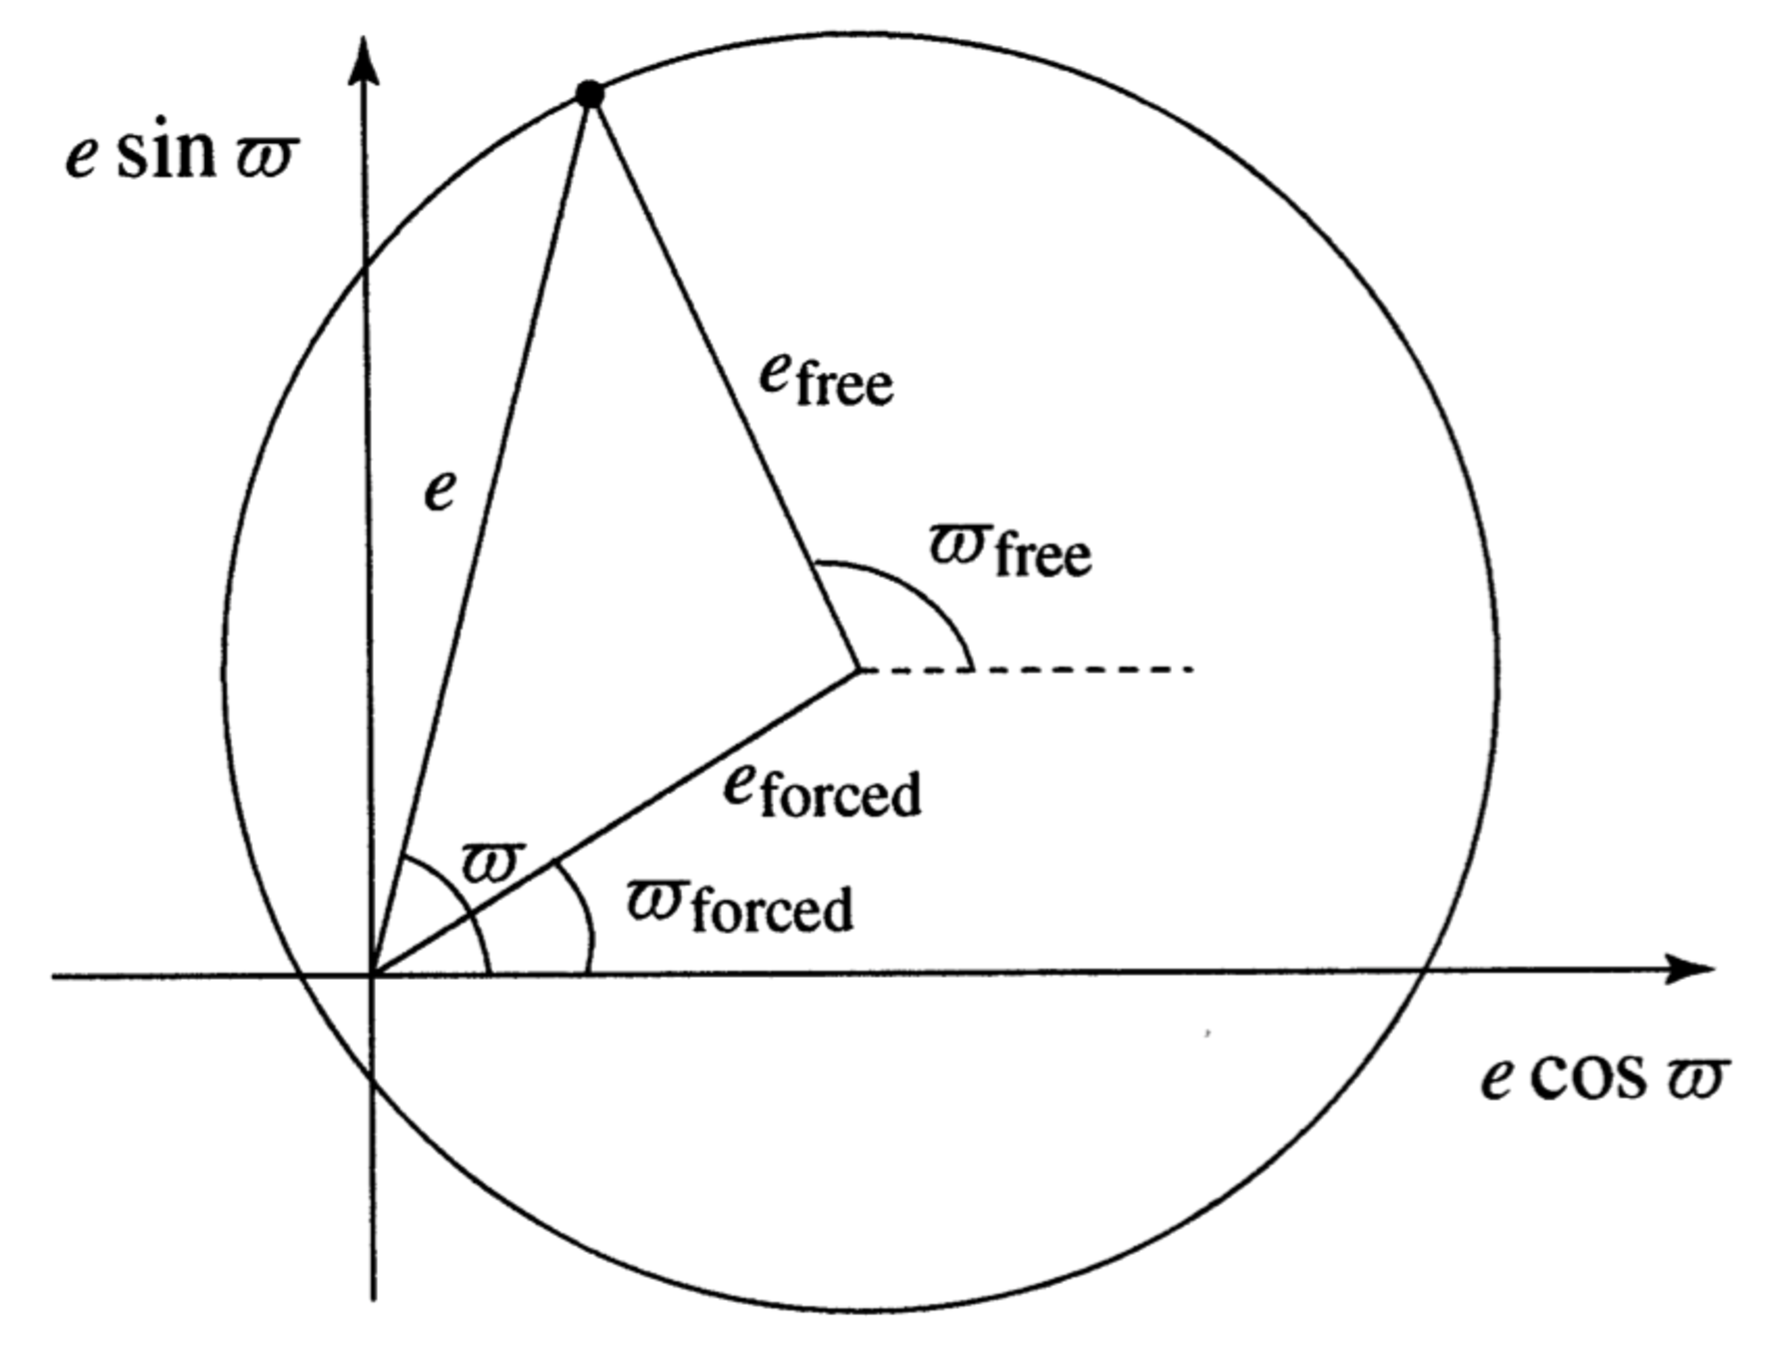
\includegraphics[width=8cm]{./image/sec7_2.pdf}
\caption{$e_{\rm free} > e_{\rm forced}$ の場合の自由離心率,強制離心率の接触要素と自由近日点経度,強制近日点経度の接触要素の関係.(Solar System Dynamics\cite{SSD} より引用)\label{fig:geometrical_e}}
\end{figure}

\begin{figure}[H]
\centering
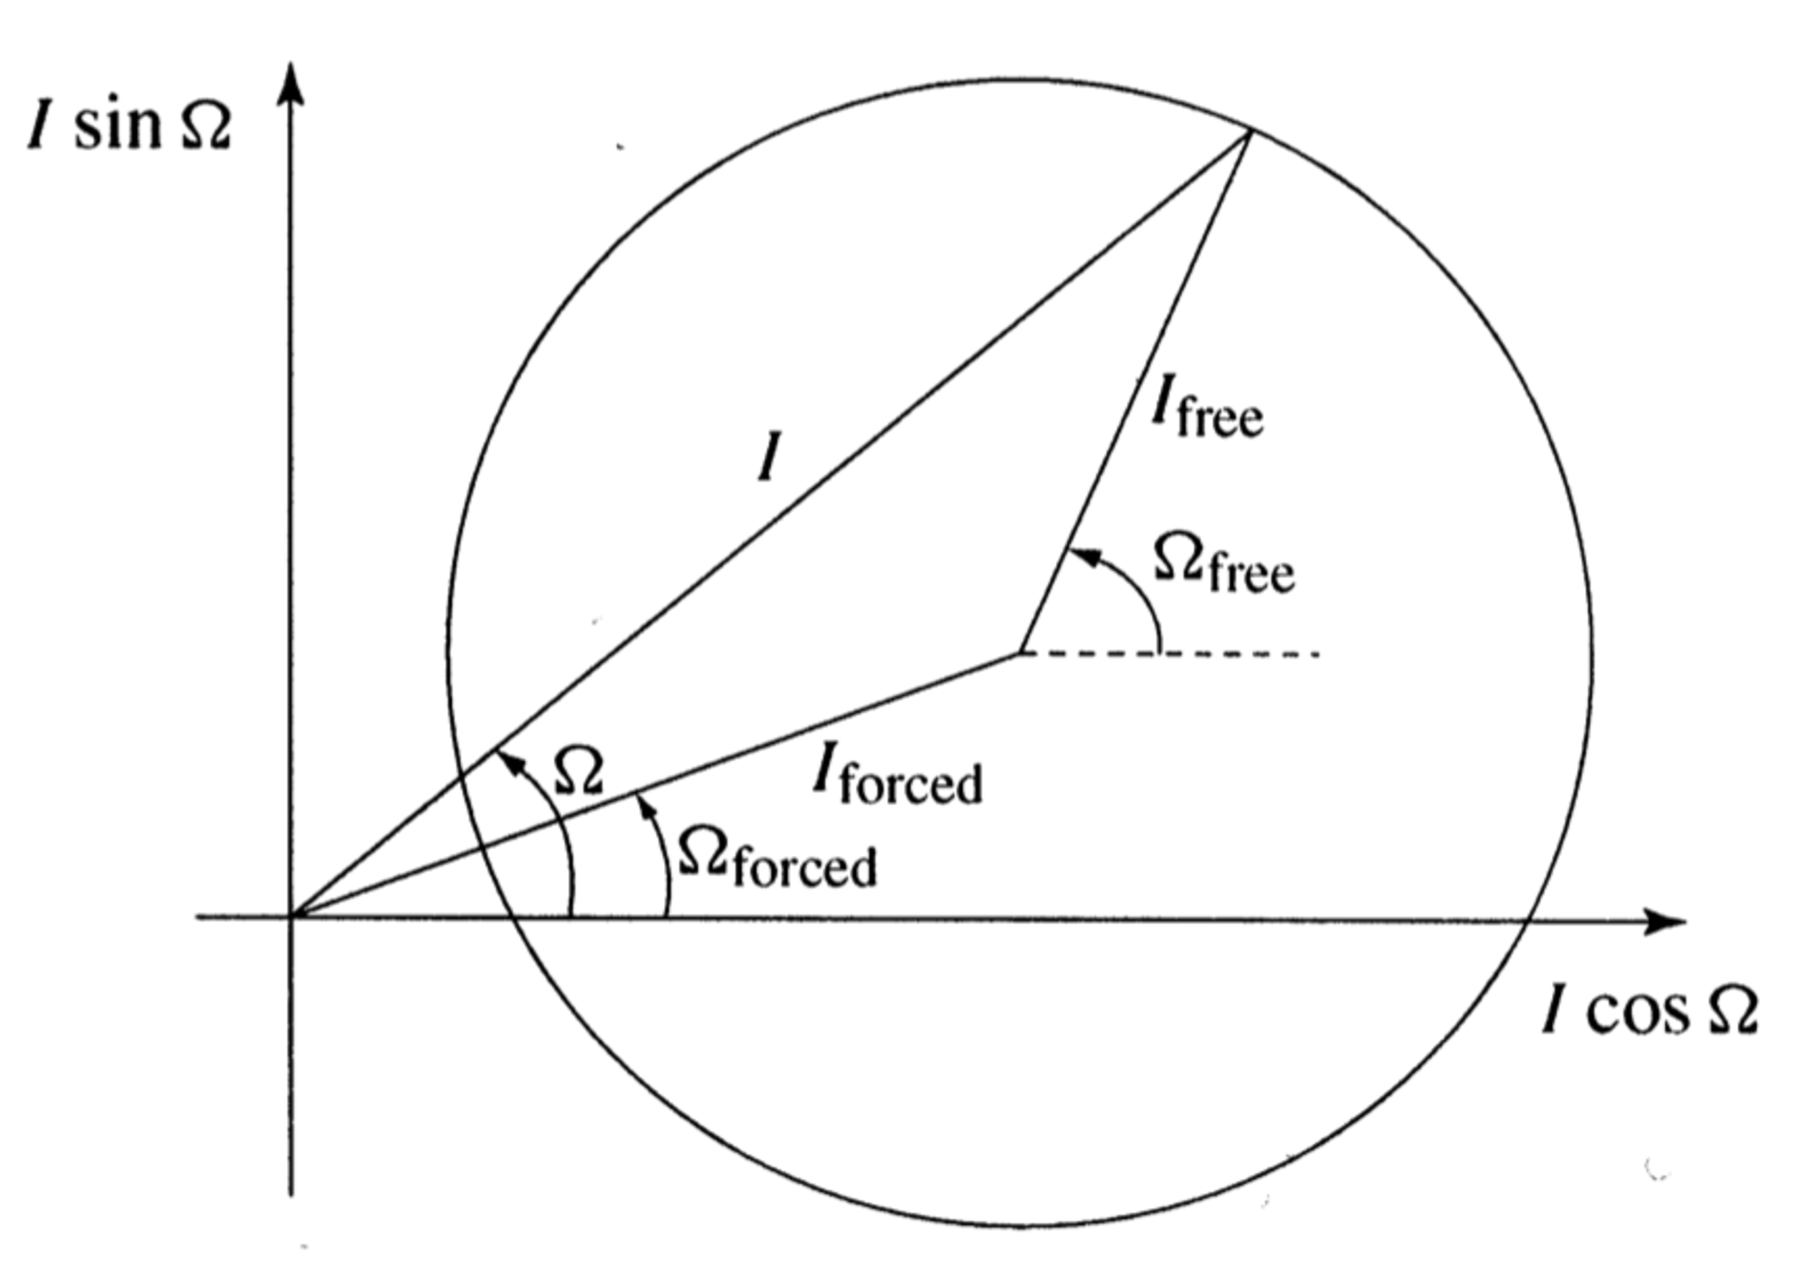
\includegraphics[width=8cm]{./image/sec7_3.pdf}
\caption{$I_{\rm free} < I_{\rm forced}$ の場合の自由軌道傾斜角,強制軌道傾斜角の接触要素と自由昇交点経度,強制昇交点経度の接触要素の関係.(Solar System Dynamics\cite{SSD} より引用)\label{fig:geometrical_I}}
\end{figure}

図\ref{fig:geometrical_e}の円は原点を含む必要がないことに注意することが重要である.$e_{\rm free}$ が十分小さい,または $e_{\rm forced}$ が十分大きい場合,粒子の円運動は,ある固定された角度の範囲の中で $\varpi$(接触近日点経度)または $\Omega$(接触昇交点経度)が変化するようなものになるだろう.

$p - q$ 解は図\ref{fig:geometrical_I}に示している.ここで $I_{\rm forced}$,$I_{\rm free}$,$\Omega_{\rm forced}$,$\Omega_{\rm free}$ は粒子の強制,自由軌道傾斜角,また強制,自由昇交点経度を表している.この図は,強制軌道傾斜角が自由軌道傾斜角より大きく,円が原点を含んでいないような状況である.上で述べたように,このことは境界条件の結果である.

式(\ref{eq:forced})の $e_{\rm forced}, I_{\rm forced}$ は,式(\ref{eq:h_0})から式(\ref{eq:q_0})の $h_0, k_0, p_0, q_0$ の定義に依存しているため,$A - g_i \approx 0$ または $B - f_i \approx 0$ のどちらかを満たす状況では $e_{\rm forced}, I_{\rm forced}$ の値が大きくなることは明らかである.$g_i, f_i$ は2つの引き合う天体の系の固有振動数である一方で,式(\ref{eq:A_test}),式(\ref{eq:B_test})より,物理量 $A, B$ はテスト粒子の軌道長半径の関数である. このことは,ある軌道長半径の場所で強制離心率または強制軌道傾斜角の発散が存在することを示している.

もう一つ重要なことは,2つの摂動源のどちらかの軌道に近づくにつれて $e_{\rm forced}, I_{\rm forced}$ が上限値に近づくことである.式(\ref{eq:nu_mu})の $\nu_i, \mu_i$ の定義と同様に,式(\ref{eq:A_test})から式(\ref{eq:B_j_test})の $A, A_j, B, B_j$ はラプラス係数 $b_{3/2}^{(1)} (\alpha_j), b_{3/2}^{(2)} (\alpha_j)$ を含み,ラプラス係数は $\alpha_j \rightarrow 1$ で無限大に発散するため,摂動源の軌道で $e_{\rm forced}, I_{\rm forced}$ が有限の上限値が存在するかは明らかではない.添字 $j = l$ で示される摂動源の軌道の付近での $e_{\rm forced}$ の振る舞いを考えていると仮定しよう.この場合,
\begin{equation}
b_{3/2}^{(1)} (\alpha_l) \rightarrow \infty \quad {\rm and} \quad b_{3/2}^{(2)} (\alpha_l) \rightarrow \infty \quad {\rm as} \quad \alpha_l \rightarrow 1.
\end{equation}
摂動源の軌道で $A \gg g_i (i = 1, 2)$ であり,$A_l \gg A_i (i \not= l)$ である.したがって,
\begin{equation}
A - g_i \approx A \approx \frac{1}{4} n \frac{m_l}{m_c} \alpha_l \bar{\alpha}_l b_{3/2}^{(1)} (\alpha_l)
\end{equation}
そして,
\begin{equation}
\nu_i = \sum_{j = 1}^{2} A_j e_{ji} \approx A_l e_{li}.
\end{equation}
これにより,
\begin{equation}
h_0 (t) \approx - \sum_{i = 1}^{2} \frac{A_l e_{li}}{A} \sin (g_i t + \beta_i) = + \frac{b_{3/2}^{(2)} (\alpha_l)}{b_{3/2}^{(1)} (\alpha_l)} \sum_{i = 1}^{2} e_{li} \sin (g_i t + \beta_i).
\end{equation}
ラプラス係数の定義から,次のように書くこともできる.
\begin{equation}
\frac{1}{2} b_{s}^{(j)} (\alpha) = \frac{s (s + 1) \cdots (s + j - 1)}{j !} \alpha^j F (s, s + j, j + 1; \alpha^2)
\end{equation}
ここで $F (a, b, c; d)$ は標準超幾何関数であり,超幾何級数の特性とそれらと楕円積分との関係から,
\begin{equation}
\lim_{\alpha_l \rightarrow 1} \frac{b_{3/2}^{(2)} (\alpha_l)}{b_{3/2}^{(1)} (\alpha_l)} = \lim_{\alpha_l \rightarrow 1} \left[ \frac{5}{4} \alpha_l \frac{F (\frac{3}{2}, \frac{7}{2}, 3; \alpha_l^2)}{F (\frac{3}{2}, \frac{5}{2}, 2; \alpha_l^2)} \right] = 1
\end{equation}
したがって,
\begin{equation}
\lim_{\alpha_l \rightarrow 1} h_0 (t) = \sum_{i = 1}^2 e_{li} \sin (g_i t + \beta_i) = h_l
\end{equation}
同様に,
\begin{equation}
\lim_{\alpha_l \rightarrow 1} k_0 (t) = \sum_{i = 1}^2 e_{li} \cos (g_i t + \beta_i) = k_l
\end{equation}
ゆえに,摂動源天体 $l$ の軌道に近づくにつれて,
\begin{equation}
e_{\rm forced} = \sqrt{h_0^2 + k_0^2} \rightarrow \sqrt{h_l^2 + k_l^2} = e_l 
\end{equation}
になる.このことは,摂動源天体の軌道での強制離心率と強制近日点経度は,摂動源天体の離心率と近日点経度に等しいことを示している.上で述べたものと同じ手法を用いると,強制軌道傾斜角と強制昇交点経度についても同様な結果が示される.
%しかし,摂動源天体の軌道付近における粒子の軌道の性質について,一般化をしすぎることに注意する必要がある.
強制離心率と強制軌道傾斜角を考えてきた結果は,$e, I$ が小さい値のときにのみ有効である.

\section{共鳴摂動}
------------------------------------ 工事中 ---------------------------------------
\subsection{共鳴の幾何 (工事中)}
\subsection{共鳴の物理 (工事中)}
\subsection{軌道要素の変化 (工事中)}
\subsection{円制限3体問題における共鳴 (工事中)}
\subsection{共鳴の幅 (工事中)}






\chapter{本研究}
\thispagestyle{fancy}
\section{目的}
先行研究で使われた惑星移動モデル\cite{Malhotra}\cite{Minton}を模擬し,本当に小天体の特徴的な分布が説明できるのかを数値計算で確かめる.

\section{数値計算の方法}
N体計算でよく用いられている「4次のエルミート法」と,効率的なタイムステップの取り方である「独立タイムステップ」について理解し,自分用のコードを作ることから始める.

この節は,東京工業大学地球惑星科学専攻井田研究室で作成された,N体計算について詳しく解説したPDF\cite{Nbody}を参考にしている.
\subsection{4次のエルミート法 \label{sec:Hermite}}
\subsubsection{手順}
\begin{enumerate}
\item t での${\bm x}_j (t)$, ${\bm v}_j (t)$ ($\to {\bm x}_{0,j} , {\bm v}_{0,j}$) と加速度 ${\bm a}_j (t)$ ($\to {\bm a}_{0,j}$) とその時間微分 $\dot{{\bm a}}_j (t)$ ($\to \dot{{\bm a}}_{0,j}$) から,$t + \Delta t$ における位置と速度 (${\bm x}_{p,j} , {\bm v}_{p,j}$) を予測する.これらを予測子 (predictor) と呼ぶ.
\item 予測子を使って,加速度 ${\bm a}_{1,j}$ とその時間微分 $\dot{{\bm a}}_{1,j}$ を求める.
\item 修正子 : 必要な回数だけ (a),(b),(c) を繰り返す.
\begin{description}
\item[(a)] ${\bm a}_{0,j}$, $\dot{{\bm a}}_{0,j}$ と ${\bm a}_{1,j}$, $\dot{{\bm a}}_{1,j}$ から加速度の2階微分と3階微分 (${\bm a}_{0,j}^{(2)}$, ${\bm a}_{0,j}^{(3)}$) を計算する.
\item[(b)] ${\bm a}_{0,j}^{(2)}$, ${\bm a}_{0,j}^{(3)}$ を使い,予測子を修正する (${\bm x}_{c,j} , {\bm v}_{c,j}$).これらを修正子 (corrector) と呼ぶ.
\item[(c)] ${\bm x}_{c,j} , {\bm v}_{c,j}$ での加速度 (${\bm a}_{1,j}^{{\rm new}}$) とその時間微分 ($\dot{{\bm a}}_{1,j}^{{\rm new}}$) を計算し,(a) に戻る.
\end{description}
\item 次のステップの準備をする.3. のループの最後の ${\bm a}_{1,j}^{{\rm new}}$, $\dot{{\bm a}}_{1,j}^{{\rm new}}$ を次のステップのための ${\bm a}_{0,j}$ と $\dot{{\bm a}}_{0,j}$ に更新し,次のステップの $\Delta t$ を求める.1. に戻る.
\end{enumerate}

\subsubsection{予測子を求める}
$t + \Delta t$ での粒子の位置,速度を次のように予測する.
\begin{eqnarray}
{\bm x}_{p,j} & = & {\bm x}_{0,j} + \Delta t {\bm v}_{0,j} + \frac{\Delta t ^2}{2} {\bm a}_{0,j} + \frac{\Delta t ^3}{6} \dot{{\bm a}}_{0,j}, \\
{\bm v}_{p,j} & = & {\bm v}_{0,j} + \Delta t {\bm a}_{0,j} + \frac{\Delta t ^2}{2} \dot{{\bm a}}_{0,j}. 
\end{eqnarray}

$\Delta t$ に対して ${\bm x}_{p,j}$ は3次,${\bm v}_{p,j}$ は2次の精度.予測子全体の精度は2次なので,本来,${\bm x}_{p,j}$ も2次まででいいのだが,$\dot{{\bm a}}_{0,j}$ が与えられているので,3次まで付け加えておく.

\subsubsection{予測子から加速度と加速度の時間微分を求める}
${\bm x}_{p,j}, {\bm v}_{p,j}$ を使い,$t + \Delta t$ での加速度 ${\bm a}_{1,j}$ とその時間微分 $\dot{{\bm a}}_{1,j}$ は以下のように計算される.
\begin{eqnarray}
{\bm a}_{1,j} & = & - \sum_{k \not= j} G m_k \frac{{\bm r}_{jk}}{(r_{jk}^2 + \epsilon^2)^{3/2}}, \label{eq:a1j}\\
\dot{{\bm a}}_{1,j} & = & - \sum_{k \not= j} G m_k \left[ \frac{{\bm v}_{jk}}{(r_{jk}^2 + \epsilon^2)^{3/2}} - \frac{3 ( {\bm v}_{jk} \cdot {\bm r}_{jk} ) {\bm r}_{jk} }{(r_{jk}^2 + \epsilon^2)^{5/2}} \right]. \label{eq:a2j}
\end{eqnarray}

ここで,
\begin{eqnarray}
{\bm r}_{jk} & = & {\bm x}_{p,j} - {\bm x}_{p,k}, \\
{\bm v}_{jk} & = & {\bm v}_{p,j} - {\bm v}_{p,k}. 
\end{eqnarray}

$\epsilon$ は計算上の発散を抑えるための softning parameter で,近接相互作用について必要な計算精度に応じてとる.

${\bm a}_{1,j}$ は3次精度,$\dot{{\bm a}}_{1,j}$ は2次精度である.

\subsubsection{${\bm a}^{(2)}, {\bm a}^{(3)}$ を求める}
Taylor 展開により,
\begin{eqnarray}
{\bm a}_{1,j} & = & {\bm a}_{0,j} + \Delta t \dot{{\bm a}}_{0,j} + \frac{\Delta t ^2}{2} {\bm a}_{0,j}^{(2)} + \frac{\Delta t ^3}{6} {\bm a}_{0,j}^{(3)}, \\
\dot{{\bm a}}_{1,j} & = & \dot{{\bm a}}_{0,j} + \Delta t {\bm a}_{0,j}^{(2)} + \frac{\Delta t ^2}{2} {\bm a}_{0,j}^{(3)}. 
\end{eqnarray}
なので,この2式を逆に解くと,
\begin{eqnarray}
{\bm a}_{0,j}^{(2)} & = & \frac{- 6 ({\bm a}_{0,j} - {\bm a}_{1,j}) - \Delta t (4 \dot{{\bm a}}_{0,j} + 2 \dot{{\bm a}}_{1,j})}{\Delta t ^2}, \\
{\bm a}_{0,j}^{(3)} & = & \frac{12 ({\bm a}_{0,j} - {\bm a}_{1,j}) + 6 \Delta t (\dot{{\bm a}}_{0,j} + \dot{{\bm a}}_{1,j})}{\Delta t ^3}. 
\end{eqnarray}
を得る.

\subsubsection{予測子の修正}
この ${\bm a}_{0,j}^{(2)}, {\bm a}_{0,j}^{(3)}$ を使って,位置と速度の予測子 (${\bm x}_{p,j}, {\bm v}_{p,j}$) を以下のように修正する.
\begin{eqnarray}
{\bm x}_{c,j} (t + \Delta t) & = & {\bm x}_{p,j} (t + \Delta t) +  \frac{\Delta t ^4}{24} {\bm a}_{0,j}^{(2)} + \alpha \frac{\Delta t ^5}{120} {\bm a}_{0,j}^{(3)}, \\
{\bm v}_{c,j} (t + \Delta t) & = & {\bm v}_{p,j} (t +\Delta t) + \frac{\Delta t ^3}{6} {\bm a}_{0,j}^{(2)} + \frac{\Delta t ^4}{24} {\bm a}_{0,j}^{(3)}. 
\end{eqnarray}
ここで,普通にTaylor 展開を考えれば,$\alpha = 1$.ただし,$\alpha \not= 1$ とすることもある.この修正により,$\Delta t$ に対して,${\bm x}_j$ は5次,${\bm v}_j$ は4次の精度になる.積分全体の精度は4次.(${\bm a}_{0,j}^{(3)}$ が与えられているので,${\bm x}_j$ は5次まで書いておくが,係数には自由度がある.)

\subsubsection{修正された予測子を使って加速度および加速度の時間微分を求める}
${\bm x}_{c,j}, {\bm v}_{c,j}$ での加速度 (${\bm a}_{1,j}^{\rm new}$) とその時間微分 ($\dot{{\bm a}}_{1,j}^{\rm new}$) を計算する.これらは,式(\ref{eq:a1j}),式(\ref{eq:a2j})で,
\begin{eqnarray}
{\bm r}_{jk} & = & {\bm x}_{c,j} - {\bm x}_{c,k}, \\
{\bm v}_{jk} & = & {\bm v}_{c,j} - {\bm v}_{c,k}. 
\end{eqnarray}
とすれば求まる.

${\bm a}_{1,j}^{\rm new}, \dot{{\bm a}}_{1,j}^{\rm new}$ を ${\bm a}_{1,j}, \dot{{\bm a}}_{1,j}$ として,「${\bm a}^{(2)}, {\bm a}^{(3)}$ を求める」に戻る.必要な回数だけこれを繰り返す(iteration).このループでは ${\bm x}_{p,j}, {\bm v}_{p,j}$ は更新しないことに注意.

\subsubsection{次のステップの準備}
ループが終わったら,最後の ${\bm a}_{1,j}^{\rm new}, \dot{{\bm a}}_{1,j}^{\rm new}$ を次のステップのための ${\bm a}_{0,j}, \dot{{\bm a}}_{0,j}$ に更新する.

\ref{sec:timestep}節でも述べるが,次のステップの $\Delta t$ は,
\begin{equation}
\Delta t_j = \eta \sqrt{\frac{| {\bm a}_{1,j} | | {\bm a}_{1,j}^{(2)} | + | \dot{{\bm a}}_{1,j} | ^2}{| \dot{{\bm a}}_{1,j} | | {\bm a}_{1,j}^{(3)} | + | {\bm a}_{1,j}^{(2)} | ^2}}.
\end{equation}
で与えることが多い.$\eta$ は積分の精度を決めるパラメータで,1より小さな数で与える (例えば,$\eta = 0.01 - 0.05$).$\eta$ を小さくすると積分精度が良くなるが,計算は遅くなる.必要な精度を満たすようになるべく小さく,一方,計算時間が長くならないようになるべく大きく,という観点で最適な $\eta$ を選ぶ.

加速度の2階微分 (${\bm a}_{1,j}^{(2)}$) と 3階微分 (${\bm a}_{1,j}^{(3)}$) は,
\begin{eqnarray}
{\bm a}_{1,j}^{(3)} & = & {\bm a}_{0,j}^{(3)}, \\
{\bm a}_{1,j}^{(2)} & = & {\bm a}_{0,j}^{(2)} + {\bm a}_{0,j}^{(3)} \Delta t. 
\end{eqnarray}
のように見積もる.これは3次の精度で正しい.(Individual timestep ではこのまま進み,Shared timestep では $\Delta t_j$ で最小のものを $\Delta t$ とする.(\ref{sec:timestep} 参照))

そして,「予測子を求める」に戻る.

$t = 0$ では,加速度の2階微分と3階微分は計算できないので,${\bm x}_j,{\bm v}_j$ での加速度 (${\bm a}_{0,j}$) とその時間微分を求め,
\begin{equation}
\Delta t_j = \eta \frac{|{\bm a}_j|}{|\dot{{\bm a}}_j|}.
\end{equation}
のようにしてから,「予測子を求める」に戻る.

\subsection{中心星重力}
中心星の周りに微惑星が回っている場合,中心星重力がほとんどの時間で圧倒的に大きい場合が多いので,中心星重力を別にして計算することが多い.簡単のため,中心星 ($j = 0$) とその周りを回る2つの天体 ($j = 1, 2$) の3体問題を考える.3天体の重心を原点にとった座標系 (慣性系) での運動方程式は,
\begin{eqnarray}
{\bm a}_0 & = & G m_1 \frac{{\bm r}_1 - {\bm r}_0}{|{\bm r}_1 - {\bm r}_0|^3} + G m_2  \frac{{\bm r}_2 - {\bm r}_0}{|{\bm r}_2 - {\bm r}_0|^3}, \label{eq:a0}\\
{\bm a}_1 & = & G m_0 \frac{{\bm r}_0 - {\bm r}_1}{|{\bm r}_10- {\bm r}_1|^3} + G m_2  \frac{{\bm r}_2 - {\bm r}_1}{|{\bm r}_2 - {\bm r}_1|^3}, \label{eq:a1}\\
{\bm a}_2 & = & G m_0 \frac{{\bm r}_0 - {\bm r}_2}{|{\bm r}_0 - {\bm r}_2|^3} + G m_1  \frac{{\bm r}_1 - {\bm r}_2}{|{\bm r}_1 - {\bm 2}_0|^3}. \label{eq:a2}
\end{eqnarray}

中心星を中心とした運動方程式を作る.式(\ref{eq:a1}),式(\ref{eq:a2})から式(\ref{eq:a0})を辺々引くと,
\begin{eqnarray}
{\bm a}_1 & = & G (m_0 + m_1) \frac{{\bm r}_1}{|{\bm r}_1|^3} + G m_2 \frac{{\bm r}_1 - {\bm r}_2}{|{\bm r}_1 - {\bm r}_2|^3} - G m_2 \frac{{\bm r}_2}{|{\bm r}_2|^3}, \\
{\bm a}_2 & = & G (m_0 + m_2) \frac{{\bm r}_2}{|{\bm r}_2|^3} + G m_1 \frac{{\bm r}_2 - {\bm r}_1}{|{\bm r}_2 - {\bm r}_1|^3} - G m_1 \frac{{\bm r}_1}{|{\bm r}_1|^3}. 
\end{eqnarray}
それぞれの式の第1項が中心星からの重力,第2項が相互作用,第3項が indirect 項となっている.これらの時間微分は,
\begin{eqnarray}
\begin{split}
\dot{{\bm a}}_1 = & - G (m_0 + m_1) \left[ \frac{{\bm v}_1}{|{\bm r}_1|^3} - 3 \frac{({\bm v}_1 \cdot {\bm r}_1) {\bm r}_1}{|{\bm r}_1|^5} \right] \\
& - G m_2 \left[ \frac{{\bm v}_1 - {\bm v}_2}{|{\bm r}_1 - {\bm r}_2|^3} - 3 \frac{[({\bm v}_1 - {\bm v}_2) \cdot ({\bm r}_1 - {\bm r}_2)] ({\bm r}_1 - {\bm r}_2)}{|{\bm r}_1 - {\bm r}_2|^5} \right] \\
& - G m_2 \left[ \frac{{\bm v}_2}{|{\bm r}_2|^3} - 3 \frac{{\bm v}_2 \cdot {\bm r}_2}{|{\bm r}_2|^5} {\bm r}_2 \right], 
\end{split}
\\
\begin{split}
\dot{{\bm a}}_2 = & - G (m_0 + m_2) \left[ \frac{{\bm v}_2}{|{\bm r}_2|^3} - 3 \frac{({\bm v}_2 \cdot {\bm r}_2) {\bm r}_2}{|{\bm r}_2|^5} \right] \\
& - G m_1 \left[ \frac{{\bm v}_2 - {\bm v}_1}{|{\bm r}_2 - {\bm r}_1|^3} - 3 \frac{[({\bm v}_2 - {\bm v}_1) \cdot ({\bm r}_2 - {\bm r}_1)] ({\bm r}_2 - {\bm r}_1)}{|{\bm r}_2 - {\bm r}_1|^5} \right] \\
& - G m_1 \left[ \frac{{\bm v}_1}{|{\bm r}_1|^3} - 3 \frac{{\bm v}_1 \cdot {\bm r}_1}{|{\bm r}_1|^5} {\bm r}_1 \right].
\end{split}
\end{eqnarray}
第1項,第2項,第3項は,加速度のそれぞれの項の時間微分に対応している.

N体問題の場合に拡張して考えると,$i, j = 1, 2, 3, \cdots, N$ に対して,
\begin{eqnarray}
{\bm a}_i & = & - G m_0 \frac{{\bm r}_i}{|{\bm r}_i|^3}  + \sum_{j \not= i} G m_j \frac{{\bm r}_{ij}}{|{\bm r}_{ij} |^3} - \sum_j G m_j \frac{{\bm r}_j}{|{\bm r}_j|^3}, \label{eq:ai} \\
\dot{{\bm a}}_i & = & - G m_0 \left[ \frac{{\bm v}_i}{|{\bm r}_i|^3} - 3 \frac{({\bm v}_i \cdot {\bm r}_i) {\bm r}_i}{|{\bm r}_i|^5} \right] \nonumber \\ 
& & - \sum_{j \not= i} G m_j \left[ \frac{{\bm v}_{ij}}{|{\bm r}_{ij}|^3} - 3 \frac{[{\bm v}_{ij} \cdot {\bm r}_{ij}] {\bm r}_{ij}}{|{\bm r}_{ij}|^5} \right] - \sum_j G m_j \left[ \frac{{\bm v}_j}{|{\bm r}_j|^3} - 3 \frac{{\bm v}_j \cdot {\bm r}_j}{|{\bm r}_j|^5} {\bm r}_j \right]. \label{eq:adoti}
\end{eqnarray}
となる.ここで,
\begin{eqnarray}
{\bm r}_{ij} & = & {\bm r}_{i} - {\bm r}_{j}, \\
{\bm v}_{ij} & = & {\bm v}_{i} - {\bm v}_{j}.
\end{eqnarray}
式(\ref{eq:ai}),式(\ref{eq:adoti})の indirect 項は $i$ にはよらないので,一度計算しておけば,全ての粒子 $i$ に対して使えることに注意.

回っている天体の質量が中心星に対して非常に小さい場合は,式(\ref{eq:ai}),式(\ref{eq:adoti})の第3項の indirect 項は第1項の中心星重力項に比べて無視できる.そのようなときには第3項の indirect 項を落とし,中心星の動きは無視して,中心星重力は外場として扱うことも多い.
\begin{eqnarray}
{\bm a}_i & = & - G m_0 \frac{{\bm r}_i}{|{\bm r}_i|^3}  + \sum_{j \not= i} G m_j \frac{{\bm r}_{ij}}{|{\bm r}_{ij} |^3},  \\
\dot{{\bm a}}_i & = & - G m_0 \left[ \frac{{\bm v}_i}{|{\bm r}_i|^3} - 3 \frac{({\bm v}_i \cdot {\bm r}_i) {\bm r}_i}{|{\bm r}_i|^5} \right] - \sum_{j \not= i} G m_j \left[ \frac{{\bm v}_{ij}}{|{\bm r}_{ij}|^3} - 3 \frac{[{\bm v}_{ij} \cdot {\bm r}_{ij}] {\bm r}_{ij}}{|{\bm r}_{ij}|^5} \right].
\end{eqnarray}
このほうが計算コストはずっと軽くなる.

以下のテスト計算,本計算では,中心星重力を外場として扱うことにした.

\subsection{タイムステップ \label{sec:timestep}}
\subsubsection{Variable Timestep (可変タイムステップ)}
軌道計算の $\Delta t$ が大きすぎると数値的な誤差が大きくなり,逆に小さすぎても計算コストがかかる.したがって,取り扱う問題やその時の状態に合った $\Delta t$ を選ぶ必要がある.特に,時々刻々と状態が大きく変化するような現象 (近接相互作用など) を取り扱う場合は,$\Delta t$ を可変にするべきである.

$\Delta t$ をどのように決めればよいかを考える.ある時刻 $t$ での粒子の位置を $x (t)$ とすると,$t + \Delta t$ での位置は,
\begin{equation}
x (t + \Delta t)  =  x (t) + v (t) \Delta t + \frac{1}{2!} a (t) (\Delta t)^2 + \cdots \label{eq:xt}
\end{equation}
と書ける.数値計算では式(\ref{eq:xt})の展開を有限項で打ち切ったものを使うため,精度の良い計算をするためには,$\Delta t$ が十分小さい必要がある.1次精度,2次精度のそれぞれの $\Delta t$ に関しての条件式が得られる.
\begin{eqnarray}
1次精度 : \Delta t & \ll & \frac{|x (t)|}{|v (t)|}, \label{eq:1storder} \\
2次精度 : \Delta t & \ll & {\rm min} \left( \frac{|x (t)|}{|v (t)|}, \frac{|v (t)|}{|a (t)|} \right). \label{eq:2ndorder}
\end{eqnarray}
$\Delta t$ は常に式(\ref{eq:1storder}),式(\ref{eq:2ndorder})を満たすように決めなければならない.例えば,係数 $\eta (\ll 1)$ を用いて,時刻 $t$ での $\Delta t$ を
\begin{eqnarray}
1次精度 : \Delta t & = & \eta \frac{|x (t)|}{|v (t)|}, \label{eq:1storder} \\
2次精度 : \Delta t & = & \eta \frac{1}{\sqrt{\left( \frac{v (t)}{x (t)} \right)^2 + \left( \frac{a (t)}{v (t)} \right)^2}}. \label{eq:2ndorder}
\end{eqnarray}
ととればよい.

\ref{sec:Hermite}節のエルミート法は4次精度である.${\bm x}, {\bm v}$ の6変数の4次の場合,上と同様に考えるとタイムステップの標識が繁雑になるので,もっと簡単な近似的な表式が用いられることが多い.よく用いられる表式は,
\begin{equation}
\Delta t  =  \eta \frac{|{\bm a}|}{|\dot{{\bm a}}|},
\end{equation}
または
\begin{equation}
\Delta t  =  \eta \sqrt{\frac{| {\bm a}| | {\bm a}^{(2)} | + | \dot{{\bm a}}| ^2}{| \dot{{\bm a}}| | {\bm a}^{(3)} | + | {\bm a}^{(2)} | ^2}} \label{eq:Aarseth}
\end{equation}
である.式(\ref{eq:Aarseth})は Aarseth によるもので,簡単でありながら非常に効率がよいタイムステップの表式であることが知られている.

\subsubsection{Shared Timestep (共有タイムステップ) とその限界}
N 体計算では,各粒子 $j$ について,「Variable Timestep (可変タイムステップ)」でやったようにして,$\Delta t_j (j = 1, 2, 3, \cdots , N)$ を計算する.例えば,その最小値
\begin{equation}
\Delta t  =  {\rm min} (\Delta t_j) ; j = 1, \cdots , N
\end{equation}
を全粒子の $\Delta t$ に採用して積分すれば,精度が保てる.このようなタイムステップの決め方を「Shared Timestep」と呼ぶ.

しかしながら,粒子同士の近接相互作用や衝突がしばしば起こり,その近接相互作用や衝突が重要なプロセスになる「衝突系」の場合 (惑星形成のシミュレーションや銀河や星団の準静的進化のシュミレーションはそういう場合に対応する) では,「Shared Timestep」では非常に効率が悪い.そこで考えだされたのが,以下に述べる「Individual Timestep」である.これは「力学的に本来必要な Timestep」で切っていこうという方法である.

また,global な計算領域を持つ場合も事情は似ている.例えば水星領域から土星領域までを含む計算の場合,水星領域での太陽まわりのケプラー時間と土星領域でのそれは 100 倍も異なる.近接相互作用をしていない粒子は太陽まわりのケプラー時間に比例した Timestep で切ることになるので,「Shared Timestep」では水星領域でのケプラー時間を基準にして土星領域の計算をするので,効率が悪い.この場合も「Individual Timestep」が有効になる.

\subsubsection{Individual Timestep (独立タイムステップ) }
「Individual Timestep」では,粒子は各々別の時間 $t_j$を持ち,別々に時間発展していく.計の時間 (「system time」または「global time」) は $t_j + \Delta t_j$ が最小になる粒子 (進めた先が一番遅れている粒子) と共に進んでいく.

粒子は各々別の時間 $t_j$ での位置 ${\bm x}_j (t_j)$,速度 ${\bm v}_j (t_j)$,加速度 ${\bm a}_j (t_j)$,加速度の時間微分 $\dot{{\bm a}}_j (t_j)$ の情報を持っていて,ある与えられた精度 ($\eta$) で次に進むことができる Timestep $\Delta t_j$ が計算されているとする.

\begin{enumerate}
\item $t_j + \Delta t_j$ が最小となる粒子 $j_{{\rm sys}}$ を選び,その時間を system time $t_{{\rm sys}}$ とする.
\item $t_{{\rm sys}}$ における全ての粒子の予測子を計算する.
\item 予測子を使って,$t_{{\rm sys}}$ での $j_{{\rm sys}}$ 粒子の ${\bm a}_{j_{{\rm sys}}}(t_{j_{{\rm sys}}}), \dot{{\bm a}}_{j_{{\rm sys}}} (t_{j_{{\rm sys}}})$ を計算する.
\item $j_{{\rm sys}}$ 粒子のみを修正する.iteration をする場合も $j_{{\rm sys}}$ 粒子以外は予測子を使う.
\item 新たな $\Delta t_{j_{{\rm sys}}}$  を計算し,$t_{j_{{\rm sys}}} + \Delta t_{j_{{\rm sys}}}$ を新たな $t_{j_{{\rm sys}}}$ として更新し,ステップ1に戻る.$j_{{\rm sys}}$ 粒子以外は予測子を捨ててもとに戻る.
\end{enumerate}

N 体計算で一番計算時間がかかるのが,$\mathcal{O} (N^2)$ の相互重力計算である.予測子はすでに持っている ${\bm x}_j (t_j), {\bm v}_j (t_j), {\bm a}_j (t_j), \dot{{\bm a}}_j (t_j)$ を使って,$t_{{\rm sys}} - t_j$ の時間分だけ予測すればいいので,$\mathcal{O} (N)$ の計算である.すなわち,進める (update する) 粒子がどんなに細かい $\Delta t_j$ でステップを切っていっても,他の粒子は実際上進むことはせず,「Shared Timestep」のときのように $\mathcal{O} (N^2)$ の無駄な計算を繰り返すことはない.このことにより,「Individual Timestep」を使うと計算が大幅に加速されることがわかる.

\section{重力散乱テスト計算}
\subsection{1体のケプラー運動 (エネルギー,角運動量とタイムステップの関係)}
4次のエルミート法のプログラムコードの計算精度が,本当に4次精度になっているのかをチェックする.質量 $M_c$ の中心星のまわりをテスト粒子がケプラー運動している場合を考える.質量 $M_c$ の中心星を原点におくと,テスト粒子の運動方程式は,
\begin{equation}
\frac{d^2 {\bm r}}{d t^2} = - \frac{G M_c {\bm r}}{r^3}
\end{equation}
である.ここで,単位長さを $1 {\rm AU}$,単位時間を $1 {\rm AU}$ におけるケプラー角速度の逆数 $(\Omega |_{1 {\rm AU}})^{-1} = (G  M_c / (1 {\rm AU})^3)^{-1}$ で規格化し,運動方程式を無次元化すると,
\begin{equation}
\frac{d^2 \tilde{\bm r}}{d  \tilde{t}^2} = - \frac{\tilde{\bm r}}{\tilde{r}^3}
\end{equation}
となる.この単位系では,時間 $2 \pi$ が $1$ 年に対応する.

xy平面上で完全な円軌道($a = 1 {\rm AU}, e = 0, I = 0 {\rm rad}$)の場合と,3次元的に傾いた平面上で円軌道からわずかにずれた軌道($a = 1 {\rm AU}, e = 0.01, I = \pi / 10 {\rm rad}$)の場合の2種類の軌道でテスト計算を行い,全エネルギーと全角運動量の相対誤差を両対数グラフにプロットしたものが図\ref{fig:relative_error}である.ここでタイムステップ $\Delta t$ は可変ではなく固定とし,全計算時間は $10$,softning parameter $\epsilon = 0$,iterationはしていない.さらに,相対誤差は,その時間での値と初期値の差の絶対値を初期値の絶対値で割ったものとして計算している(正の値のみ).
\begin{figure}[H]
\centering
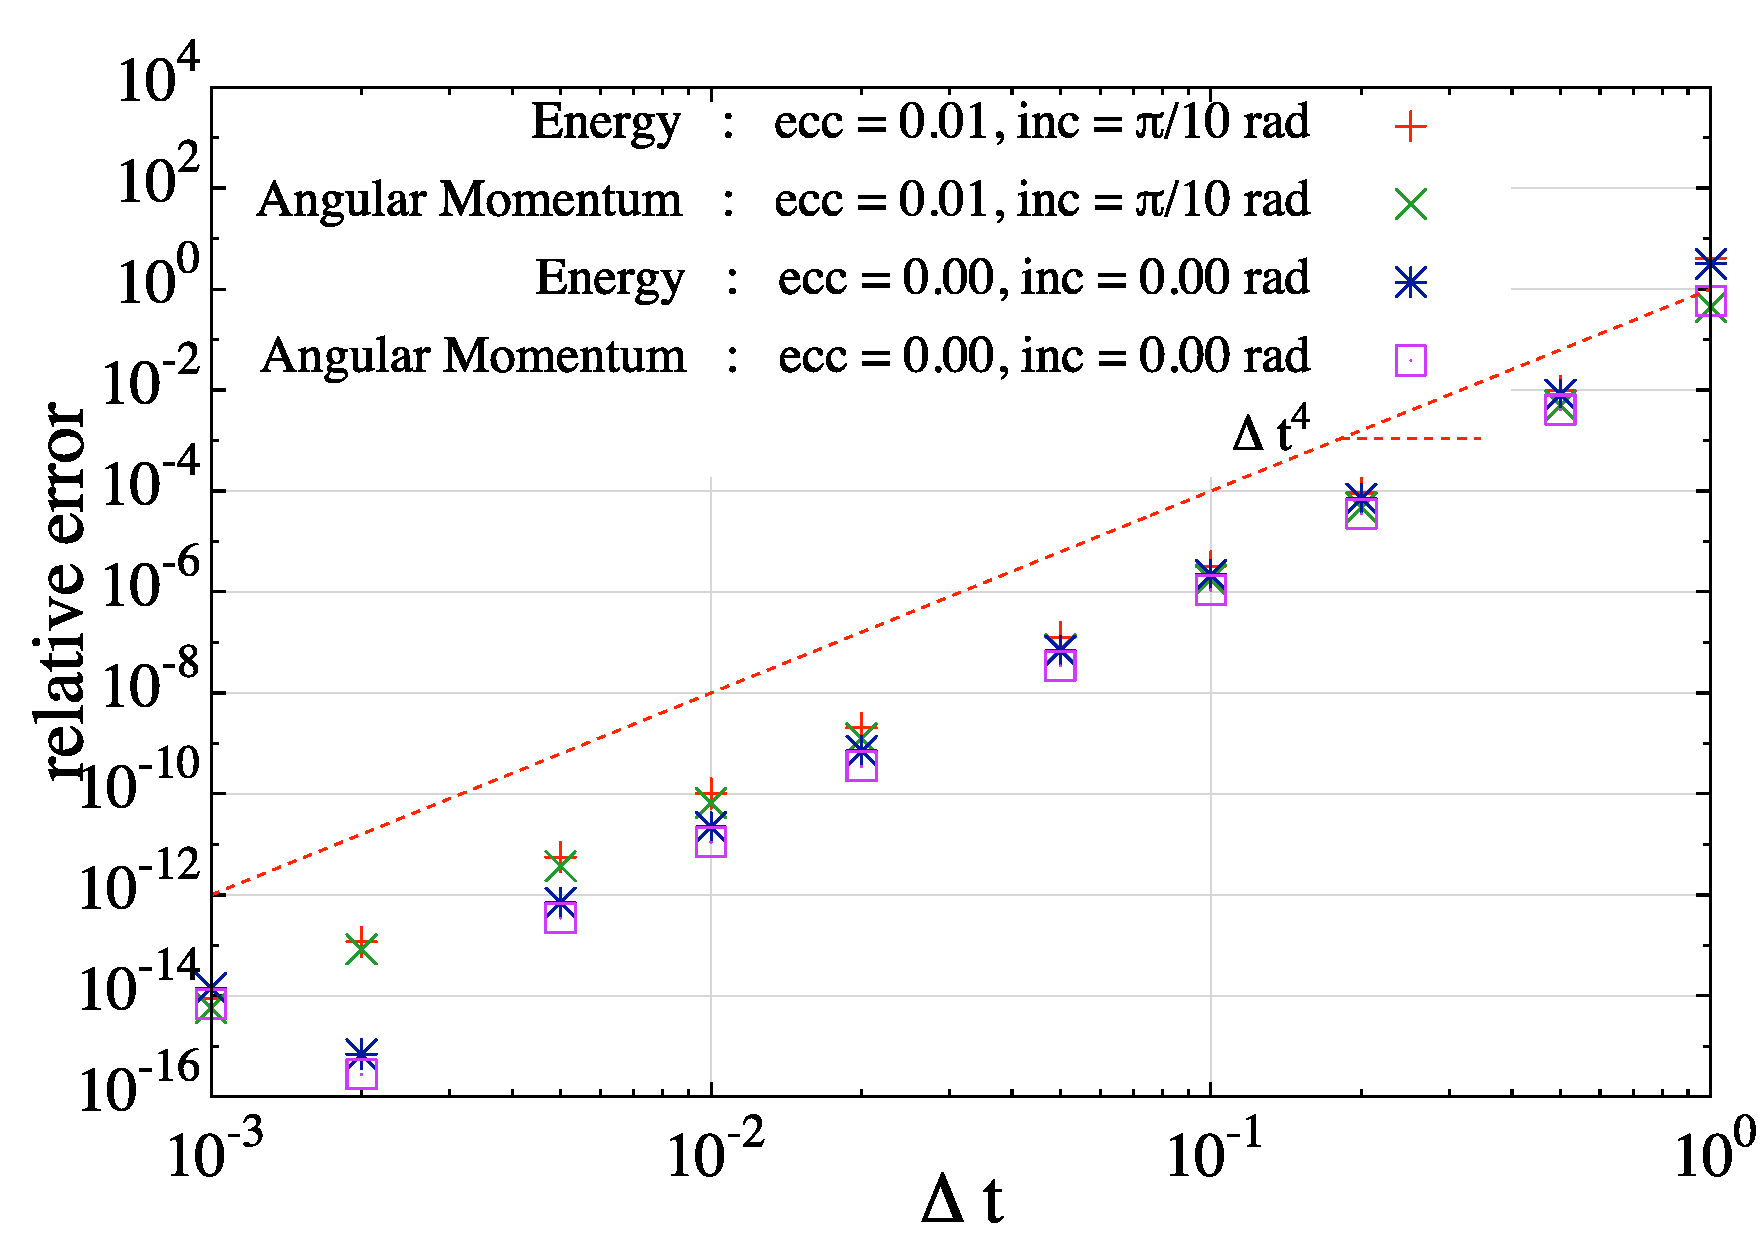
\includegraphics[width=10cm]{./image/relative_error.pdf}
\caption{テスト粒子が中心星のまわりを2種類の軌道($a = 1 {\rm AU}, e = 0, I = 0 {\rm rad}$ と $a = 1 {\rm AU}, e = 0.01, I = \pi / 10 {\rm rad}$)でケプラー運動するときの,タイムステップを変えたときの全エネルギーと全角運動量の相対誤差.比較のため,$\Delta t^4$ の曲線を並べてプロットしている.\label{fig:relative_error}}
\end{figure}
4次精度であれば,同じステップ数だけ計算したときの相対誤差は $\Delta t^5$ に比例する.また,$\Delta t$ が小さくなるにつれステップ数が $\Delta t^{-1}$ に比例して増えることから,全計算時間 $10$ 後の相対誤差は $\Delta t^4$ に比例するべきである.図\ref{fig:relative_error}より,用いたコードの積分精度は確かに4次精度を保っていることが分かる.また,相対誤差が double 型の打ち切り誤差($\sim 10^{-16}$)よりも小さくなることはなく,その下限値となる $\Delta t$ よりもタイムステップを小さくしても計算精度が上がることはない.このことも図\ref{fig:relative_error}から読み取ることができる.

\subsection{円軌道の惑星と微惑星の重力散乱}
近接相互作用がきちんと計算されるかをチェックする.ここではタイムステップは shared timestep を用い,$\eta = 0.01$,softning parameter $\epsilon = 0$,iterationは3回とした.質量 $M_c$ の中心星のまわりを,半径 $a_1$ の円軌道にある惑星(質量 $m_1 = 3 \times 10^{-6} M_c$)と,半径 $a_2$ の円軌道にある微惑星(質量 $m_2 = 1 \times 10^{-15} M_c$)がまわっているとする($a_2 > a_1$).半径が違うため角速度が異なり,いずれ惑星と微惑星は接近する.微惑星が惑星に1回だけ遭遇する場合の軌道変化を計算したいので,初期の配置は微惑星−中心星−惑星の角度が $90^{\circ}$ になるようにし,再びこの角度が $90^{\circ}$ になるとき計算終了とした.衝突パラメータ $b$ を惑星のヒル半径($r_H = (m_1 / 3 M_c)^{1/3} a_1 = 10^{-2} a_1$)で規格化し,$b = (a_2 - a_1) / r_H = (a_2 - a_1) / a_1 \times 10^2$ とする.

規格化した衝突パラメータの変化(軌道長半径の変化に対応)を $\Delta b$,微惑星の離心率の変化を $\Delta e$($(m_1 / 3 M_c)^{1/3} = 10^{-2}$ で規格化,初期は円軌道 $e = 0$ なので散乱後の $e$ と等しい),最接近距離を $r_{\rm min}$(ヒル半径 $r_H = 10^{-2} a_1$ で規格化)とする.

衝突パラメータを[1.0:3.5]の範囲で0.002ごとに変えて軌道計算をし,$\Delta b, \Delta e, r_{\rm min}$ の変化をプロットしたものが図\ref{fig:delta_b},図\ref{fig:delta_e},図\ref{fig:r_min}である.

\begin{figure}[H]
\centering
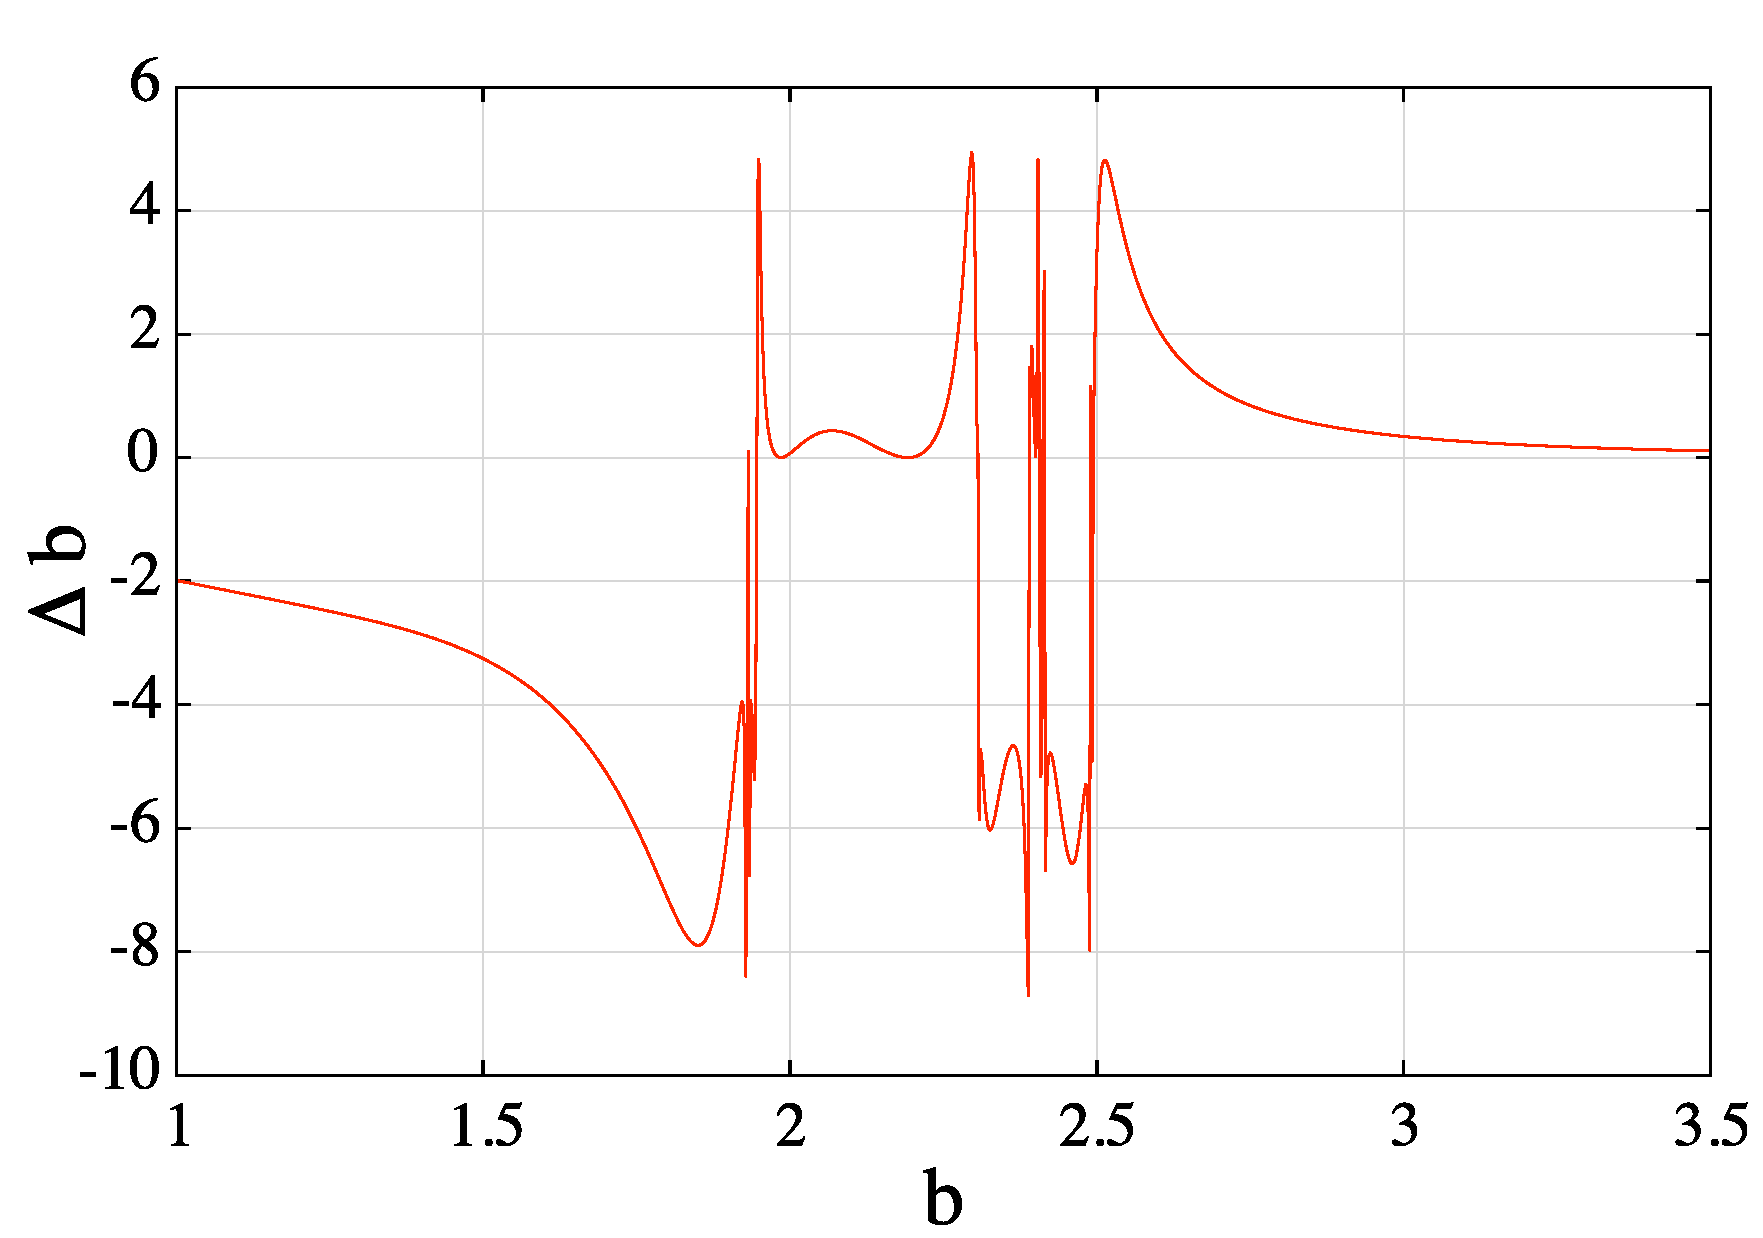
\includegraphics[width=8cm]{./image/planetesimal_delta_b.pdf}
\caption{衝突パラメータの変化 $\Delta b$.\label{fig:delta_b}}
\end{figure}

\begin{figure}[H]
\centering
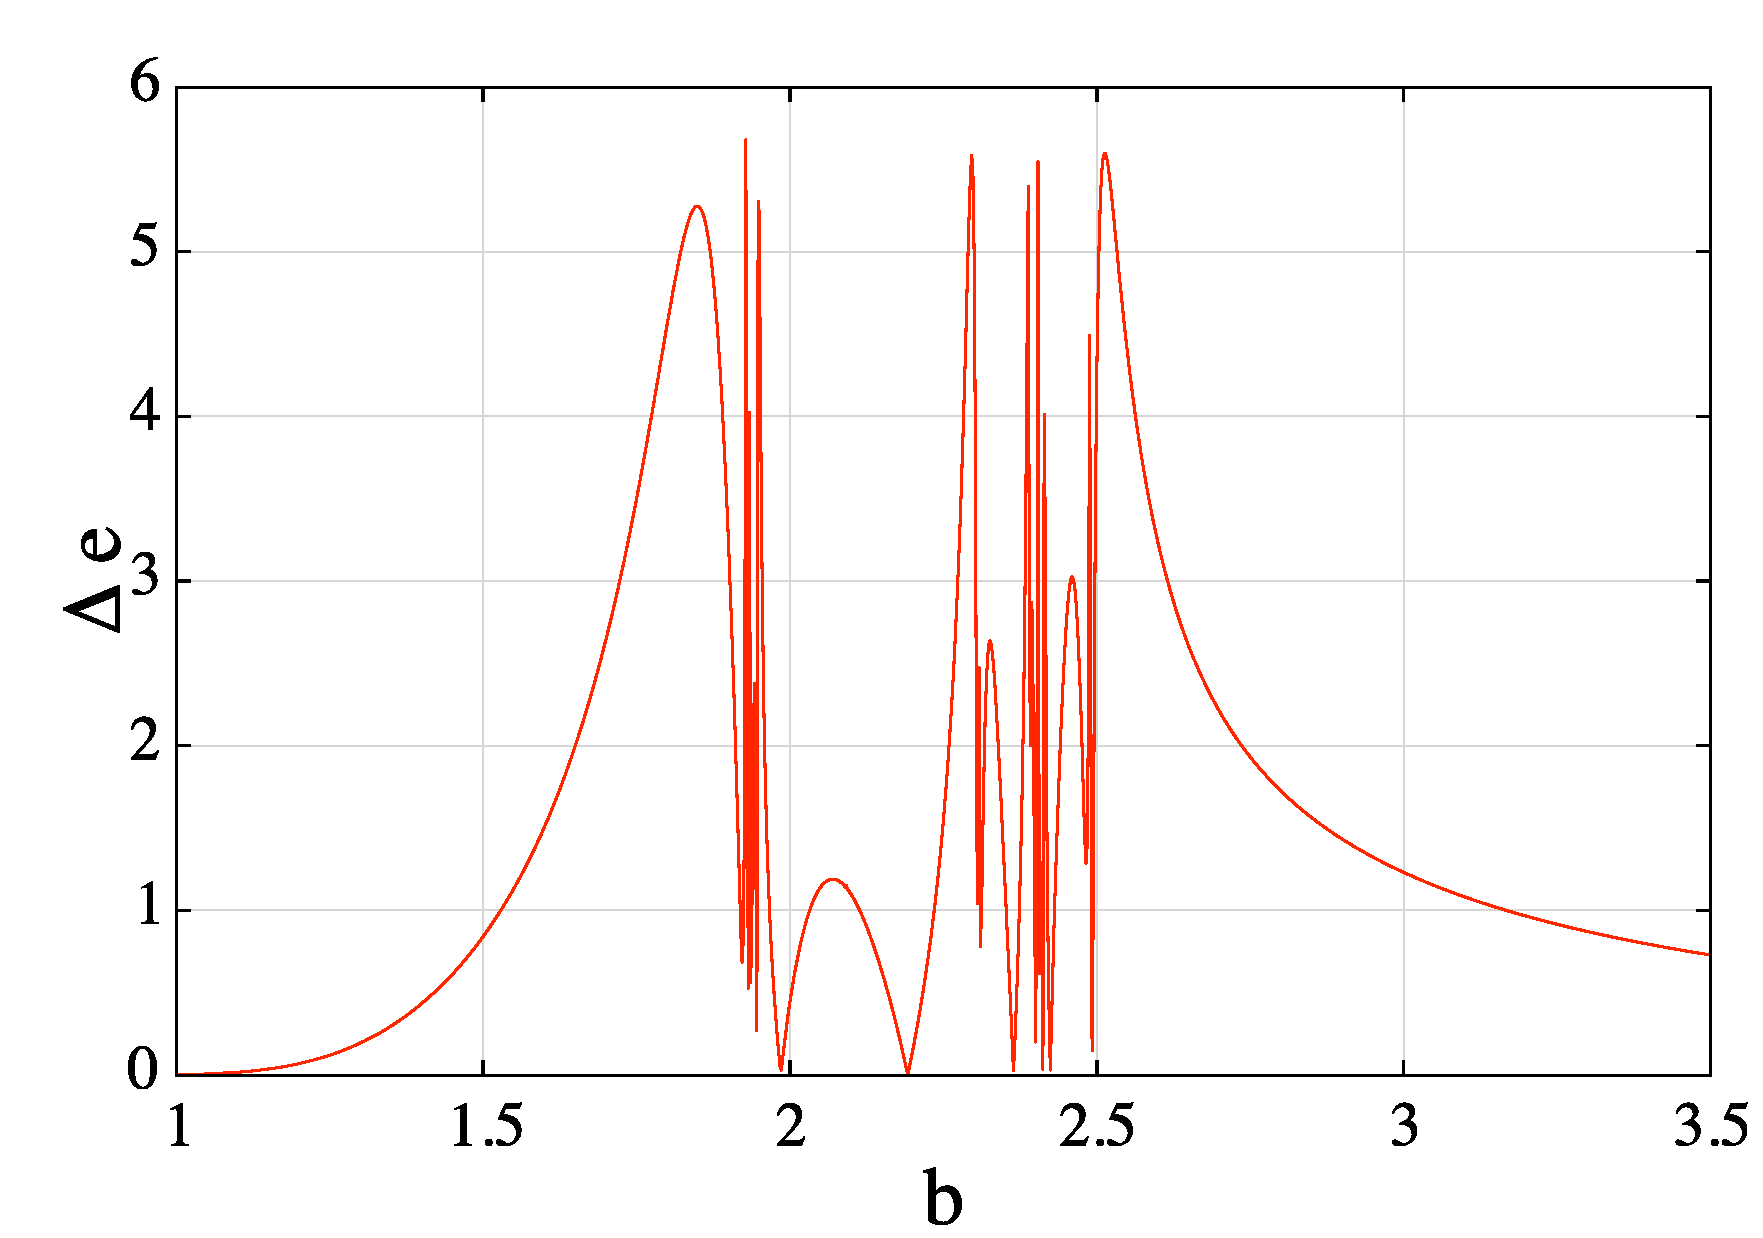
\includegraphics[width=8cm]{./image/planetesimal_delta_e.pdf}
\caption{離心率の変化 $\Delta e$($(m_1 / 3 M_c)^{1/3} = 10^{-2}$ で規格化).\label{fig:delta_e}}
\end{figure}

\begin{figure}[H]
\centering
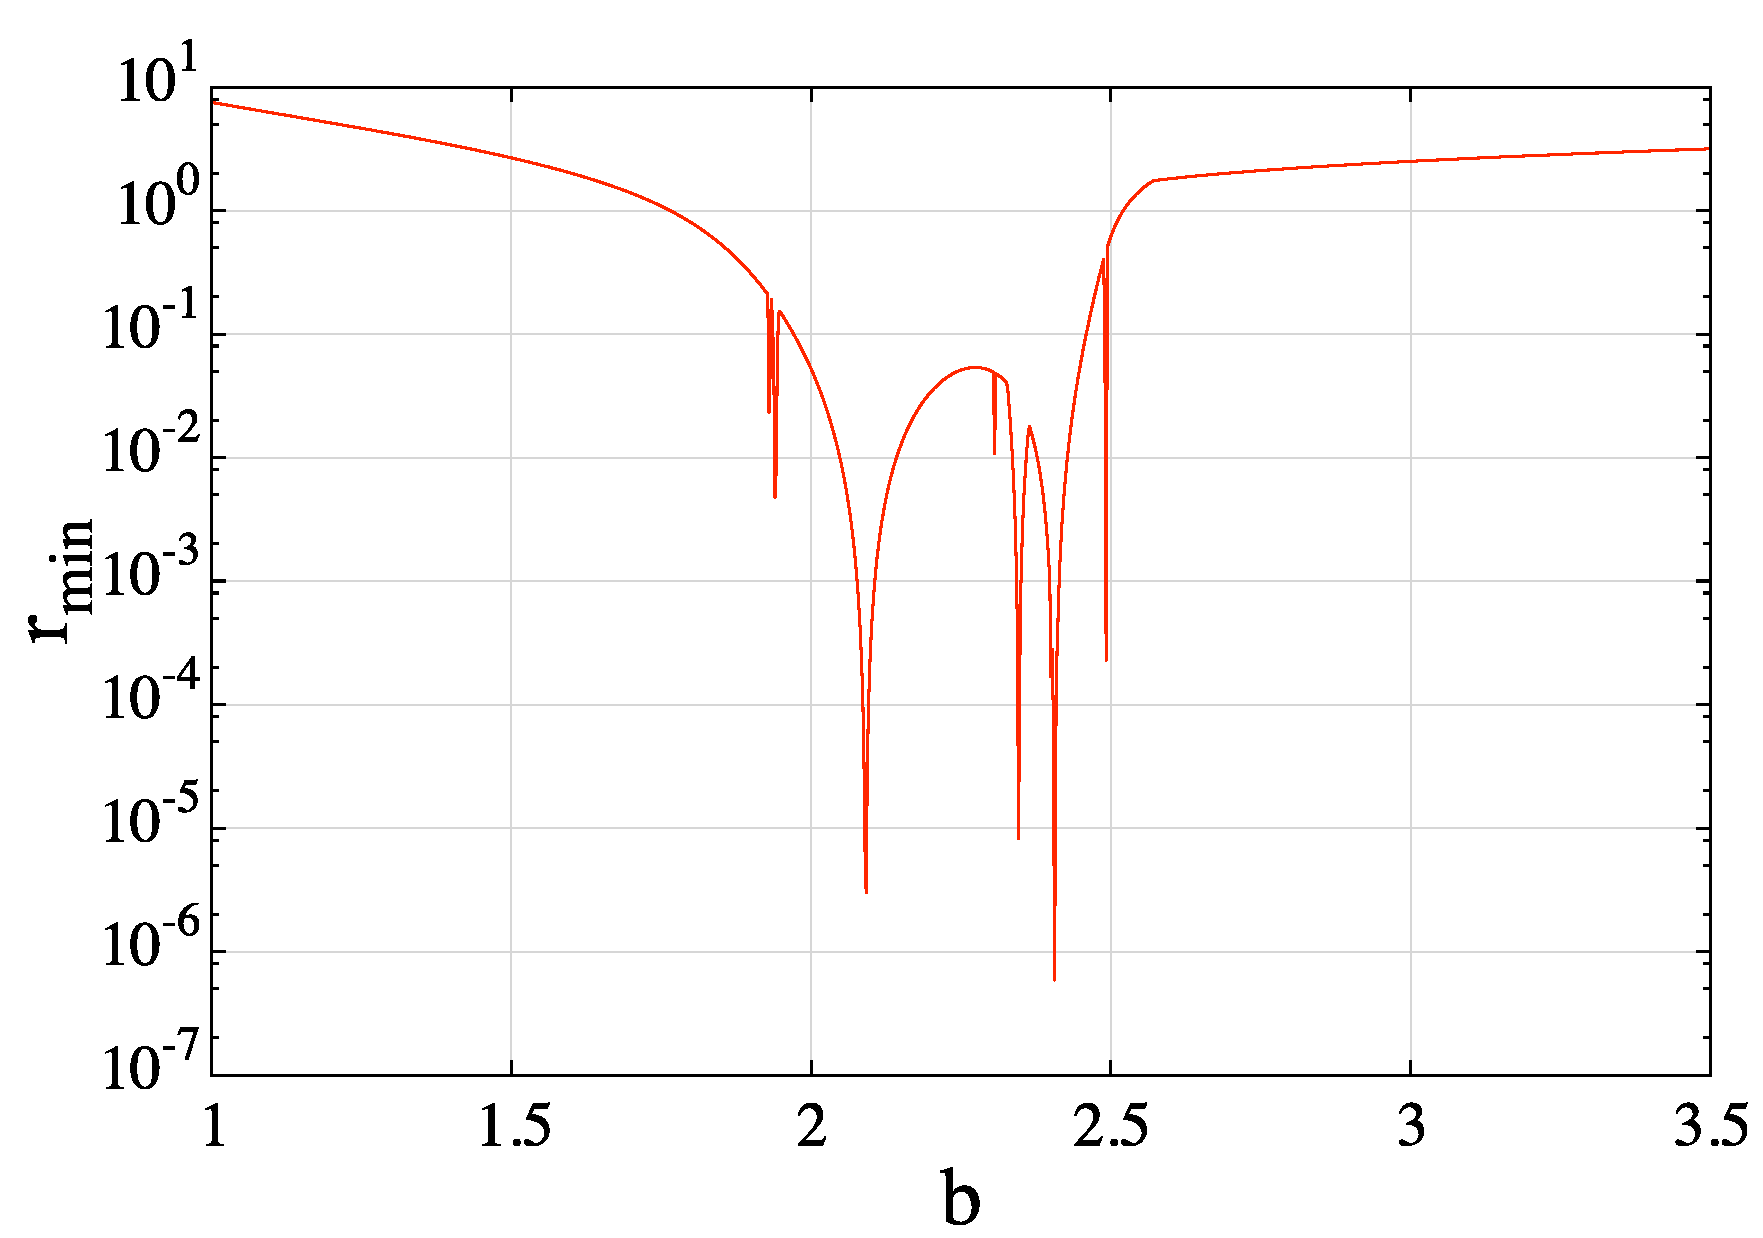
\includegraphics[width=8cm]{./image/planetesimal_r_min.pdf}
\caption{最接近距離 $r_{\rm min}$(ヒル半径 $r_H = 10^{-2} a_1$ で規格化).\label{fig:r_min}}
\end{figure}




\subsection{ピタゴラス問題}
ピタゴラス問題とは,質量 3, 4, 5 の質点を辺長 3, 4, 5 の直角三角形の頂点に静止させ,手を離したときの3体問題のことである(図\ref{fig:pythagoras}参照).1913年にC.Burrauによって研究され、1967年にSzebehelyらによって解決された問題であり,これまで詳しい数値計算が行われてきた.近接相互作用をどこまで正確に追えるかをチェックするテスト問題としてよく使われる.

\begin{figure}[H]
\centering
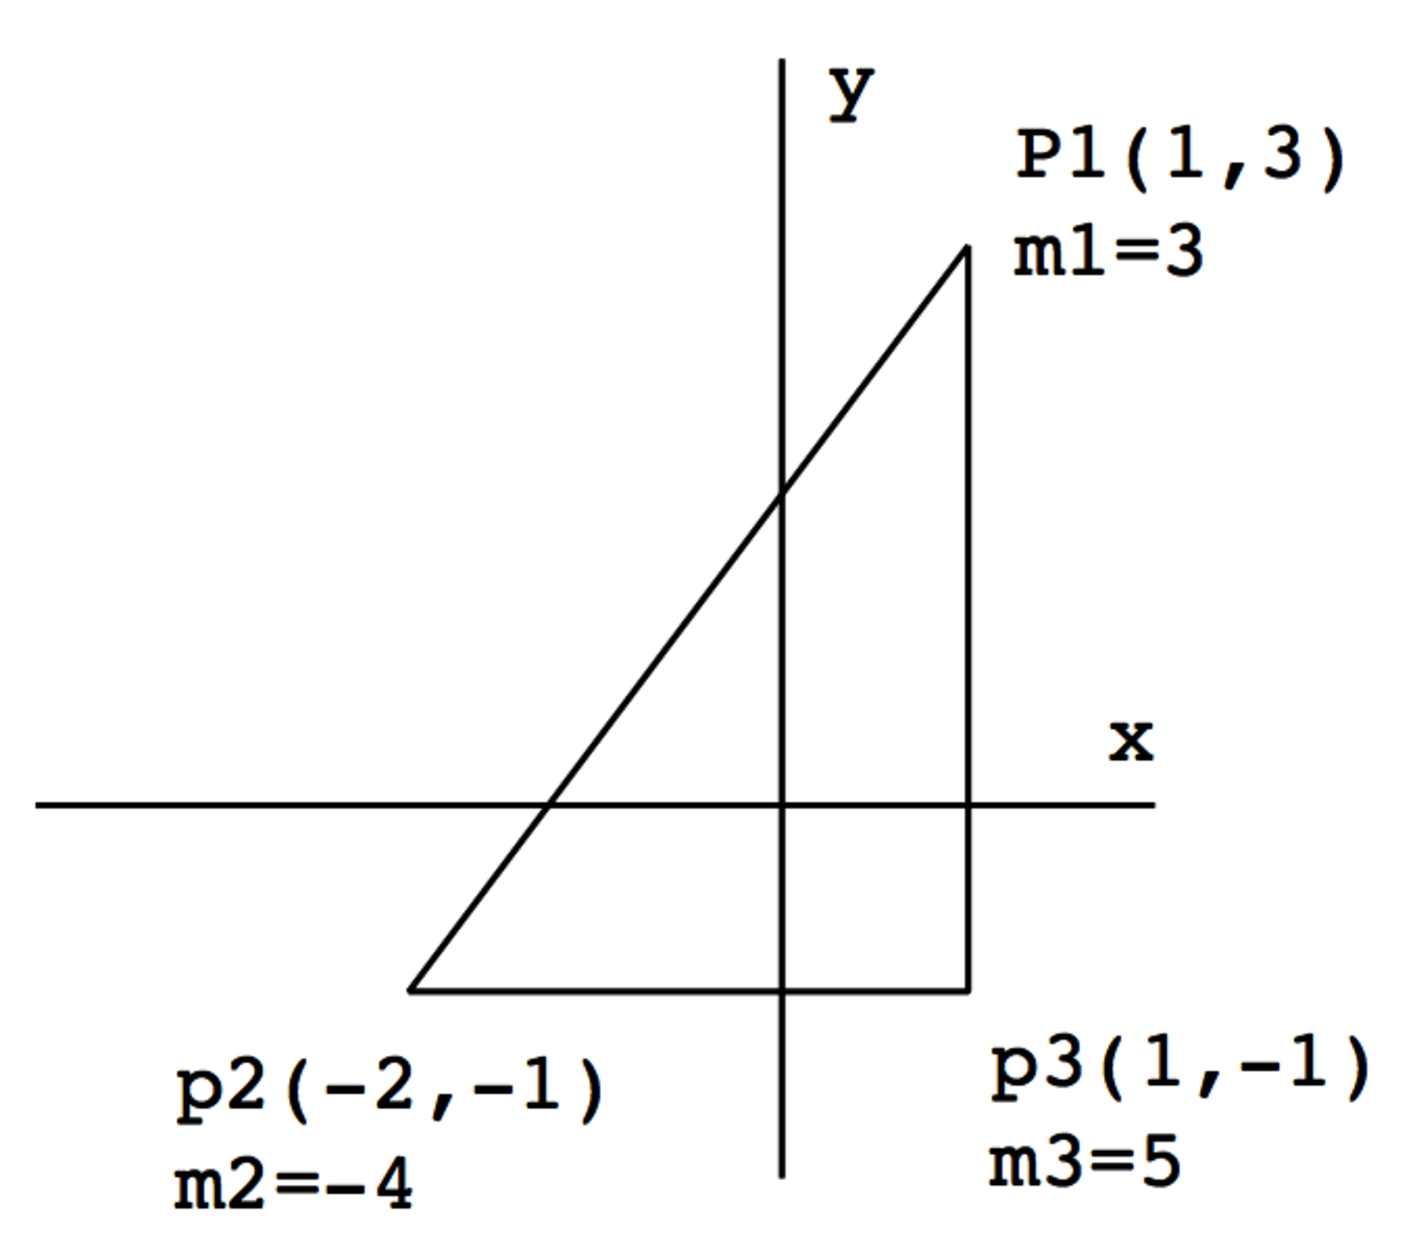
\includegraphics[width=8cm]{./image/pythagoras_1.pdf}
\caption{ピタゴラス問題の初期配置.質量 3, 4, 5 の質点を辺長 3, 4, 5 の直角三角形の頂点におく.\label{fig:pythagoras}}
\end{figure}

初期には3つの質点が静止しているため,角運動量は0であり,重心は静止している.図\ref{fig:pythagoras}のような配置をすると,原点と重心が一致する.運動方程式を,距離の単位を $L$,質量の単位を $M$,時間の単位を $T$ で無次元化すると,
\begin{equation}
\frac{G M T^2}{L^3} = 1
\end{equation}
という関係が得られるので,例えば $L = 1 {\rm AU}$,$M = 1 M_{\odot}$ とすると,時間の単位は $T = 1/(2 \pi) 年$ となる.

この計算では,タイムステップは shared timestep を用い,$\eta = 3 \times 10^{-3}$,softning parameter $\epsilon = 0$,iteration は3回とした. 計算時間は文献を参考に70までとし,$t = 10$ごとに各質点の軌道をプロットしたものが図\ref{fig:pythagoras_orbit}である.

\begin{figure}[H]
\begin{tabular}{ccc}
%左
\begin{minipage}[t]{0.45\hsize}
\centering
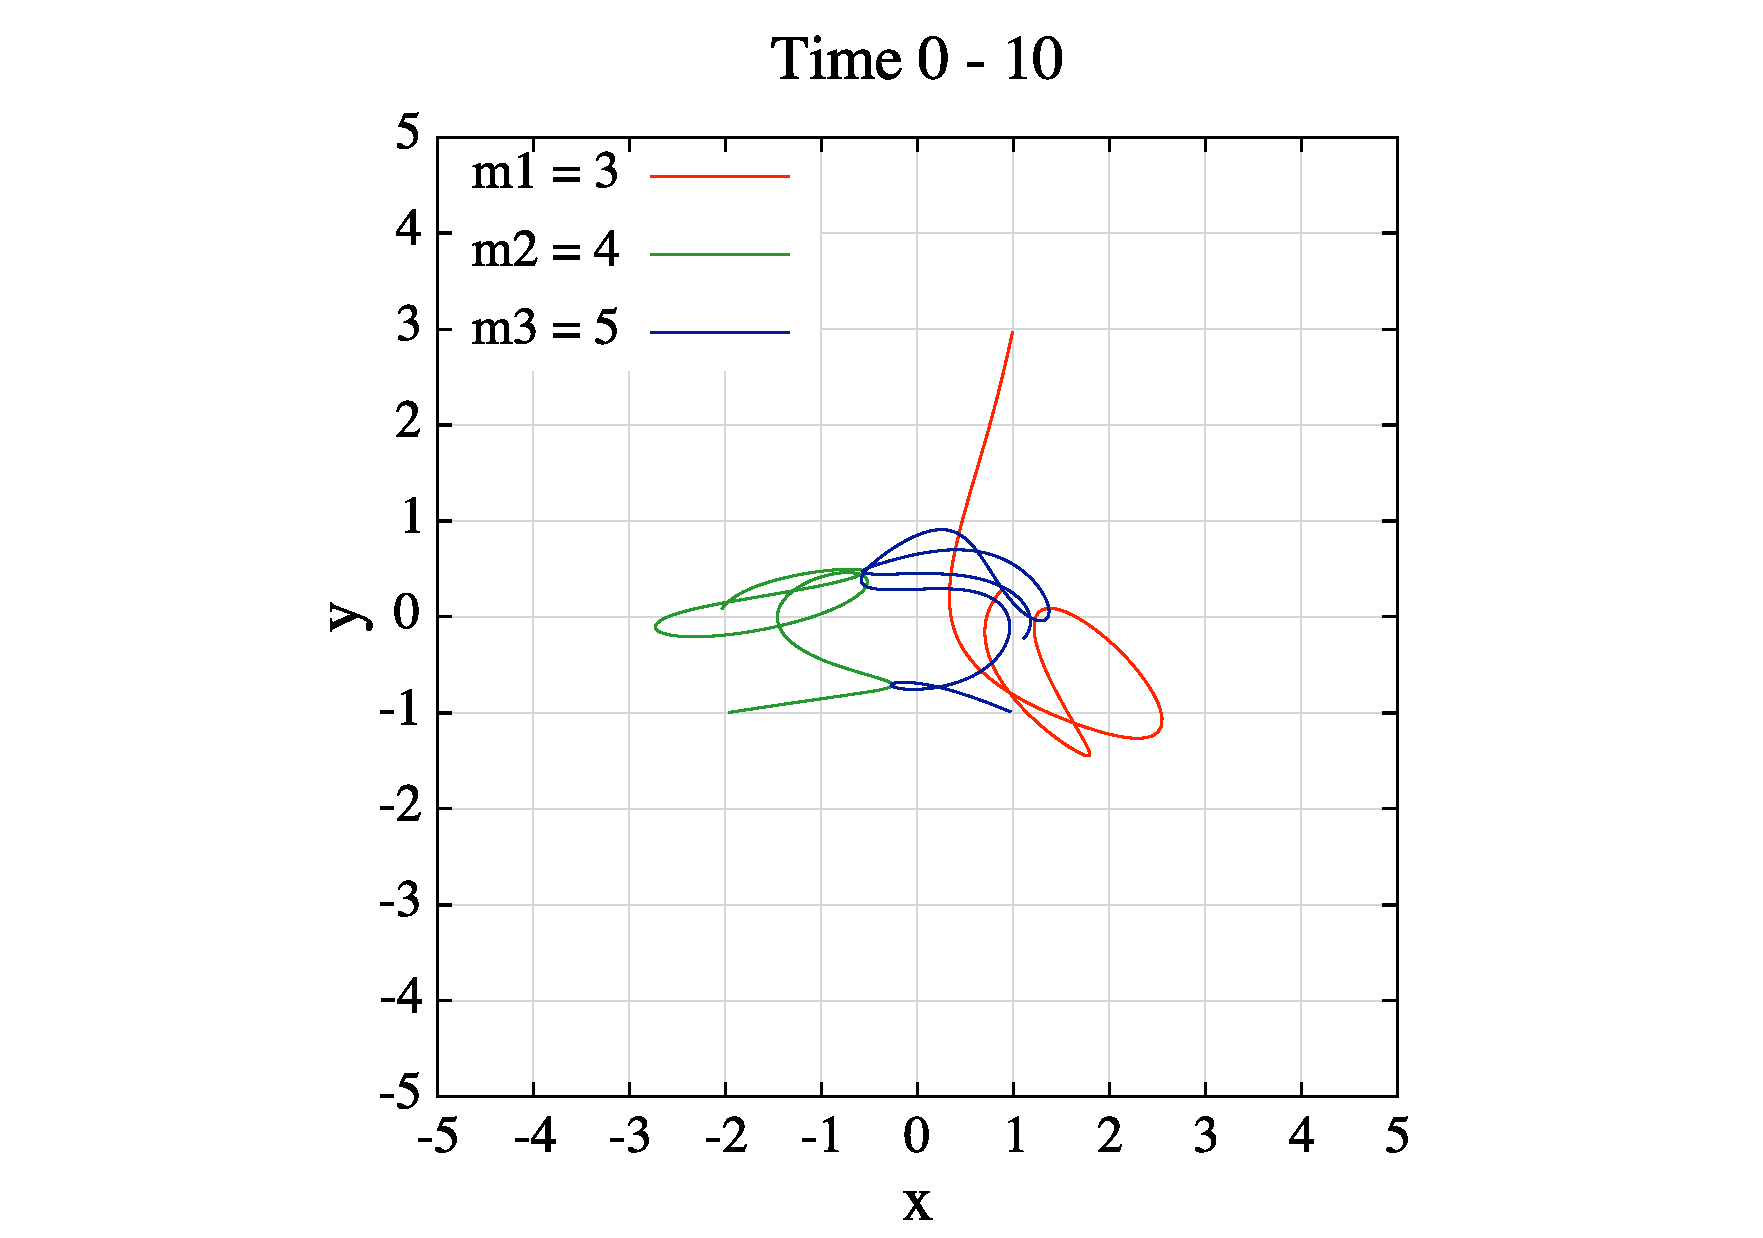
\includegraphics[width=8cm]{./image/pythagoras_orbit_0to10.pdf}
\end{minipage} &
%調整
\begin{minipage}[t]{0.1\hsize}
\end{minipage} &
%右
\begin{minipage}[t]{0.45\hsize}
\centering
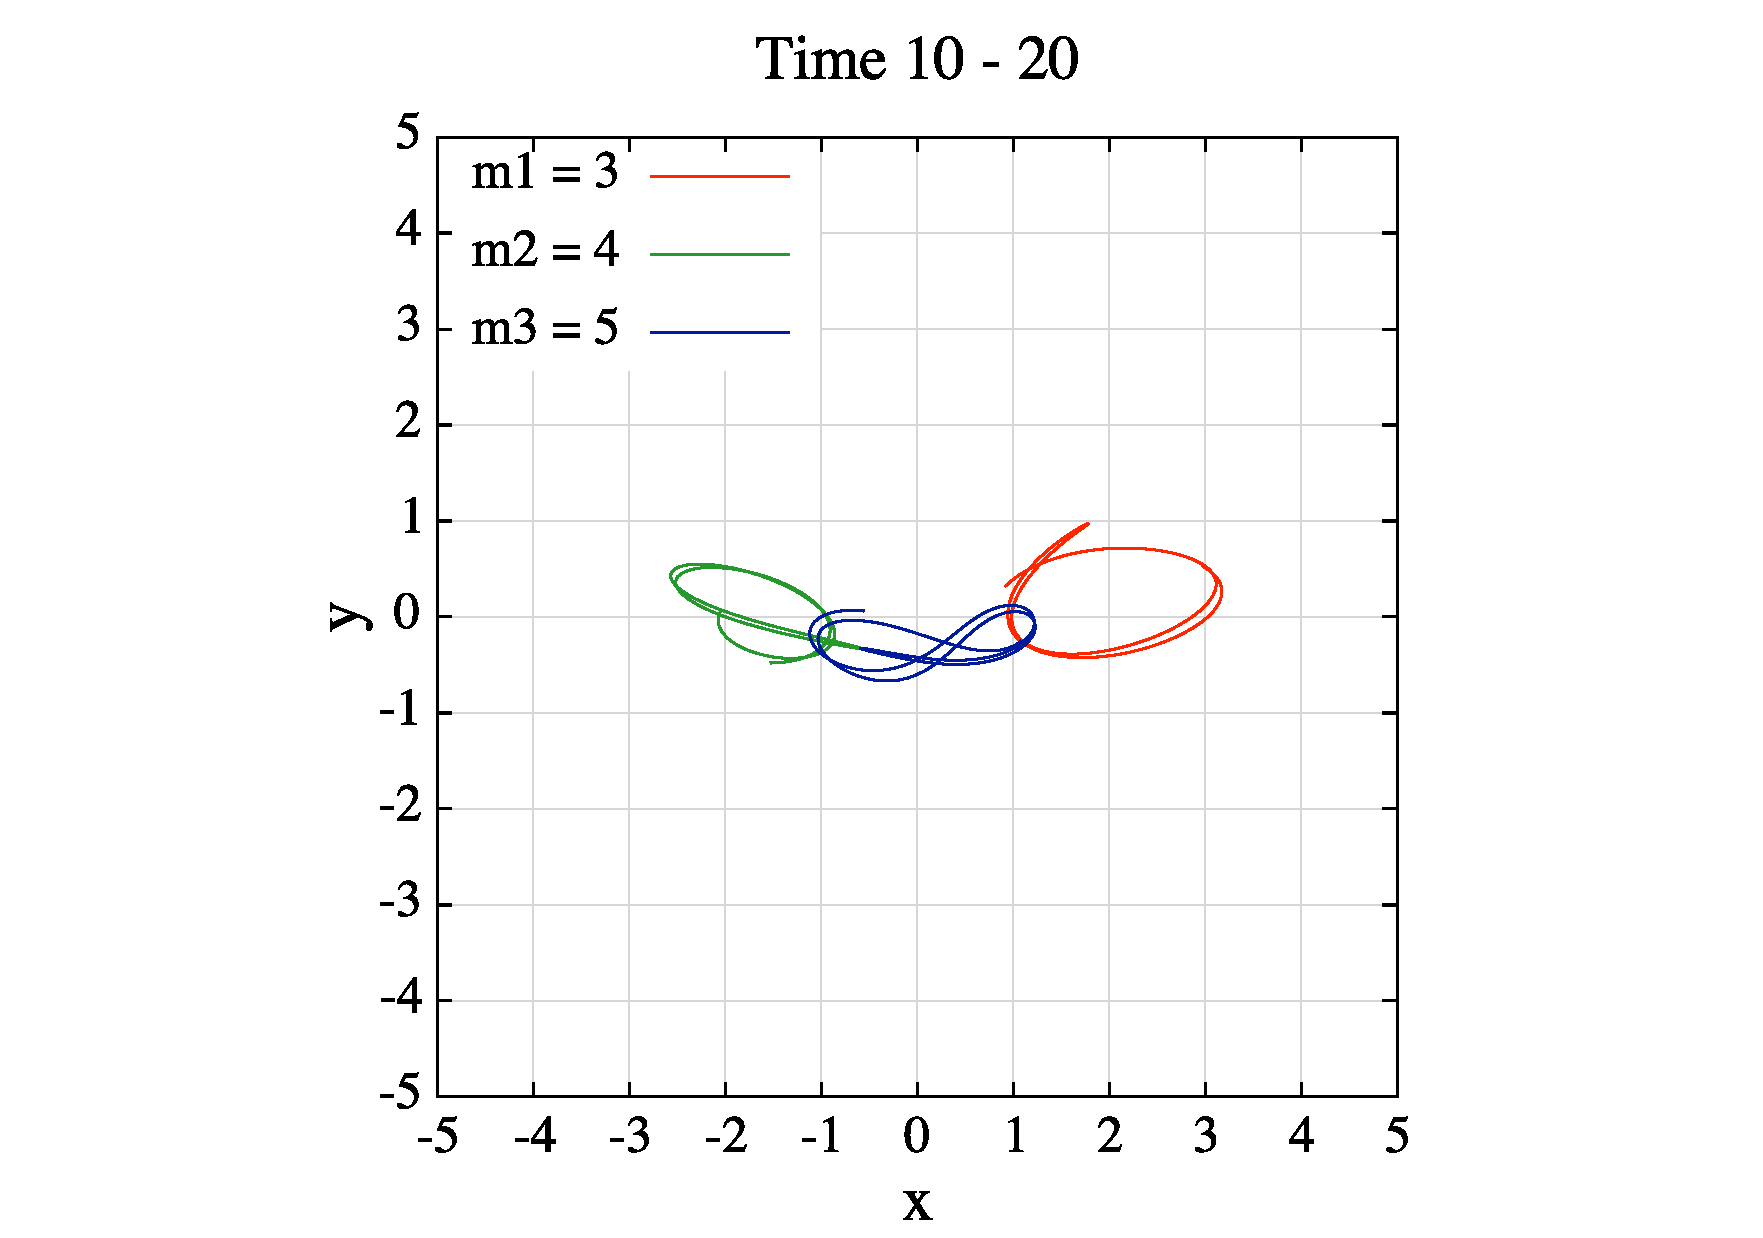
\includegraphics[width=8cm]{./image/pythagoras_orbit_10to20.pdf}
\end{minipage}\\
%
%左
\begin{minipage}[t]{0.45\hsize}
\centering
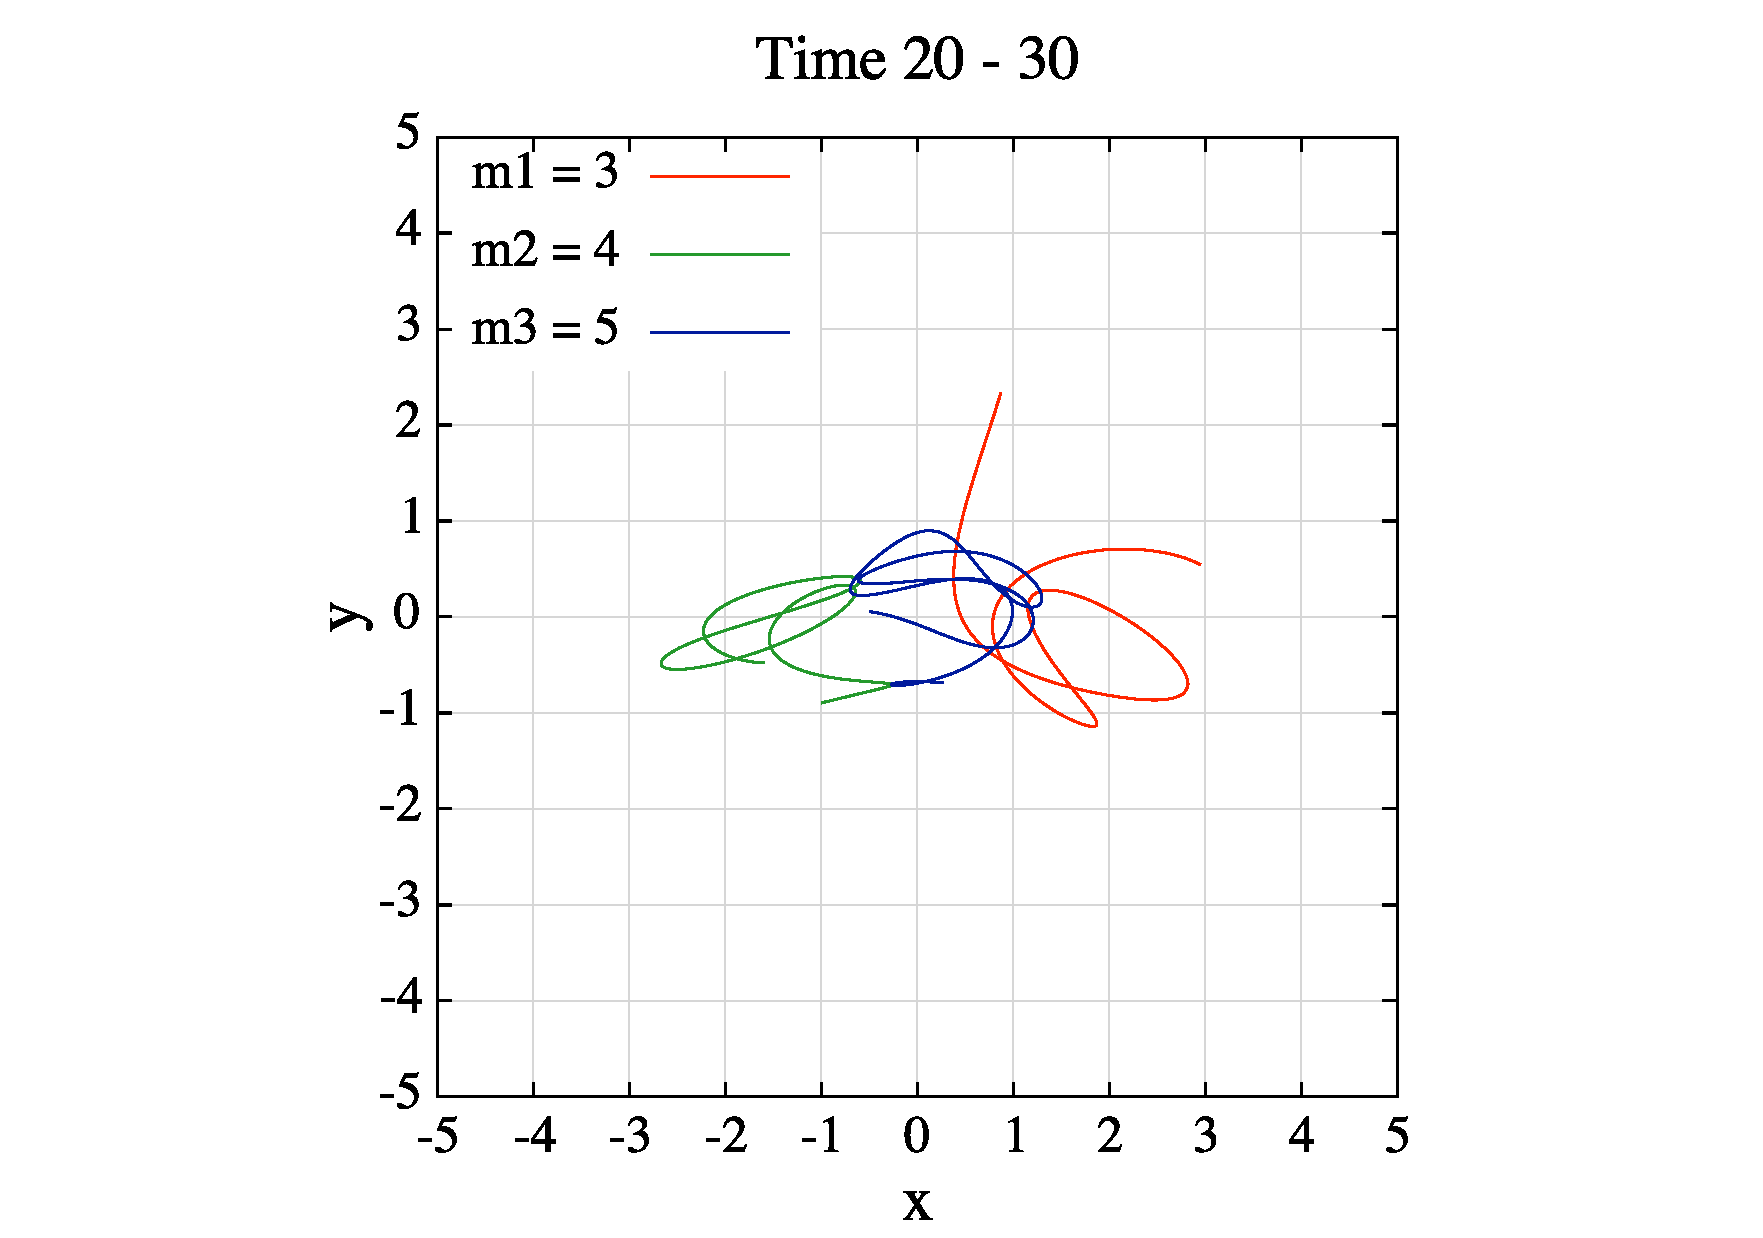
\includegraphics[width=8cm]{./image/pythagoras_orbit_20to30.pdf}
\end{minipage} &
%調整
\begin{minipage}[t]{0.1\hsize}
\end{minipage} &
%右
\begin{minipage}[t]{0.45\hsize}
\centering
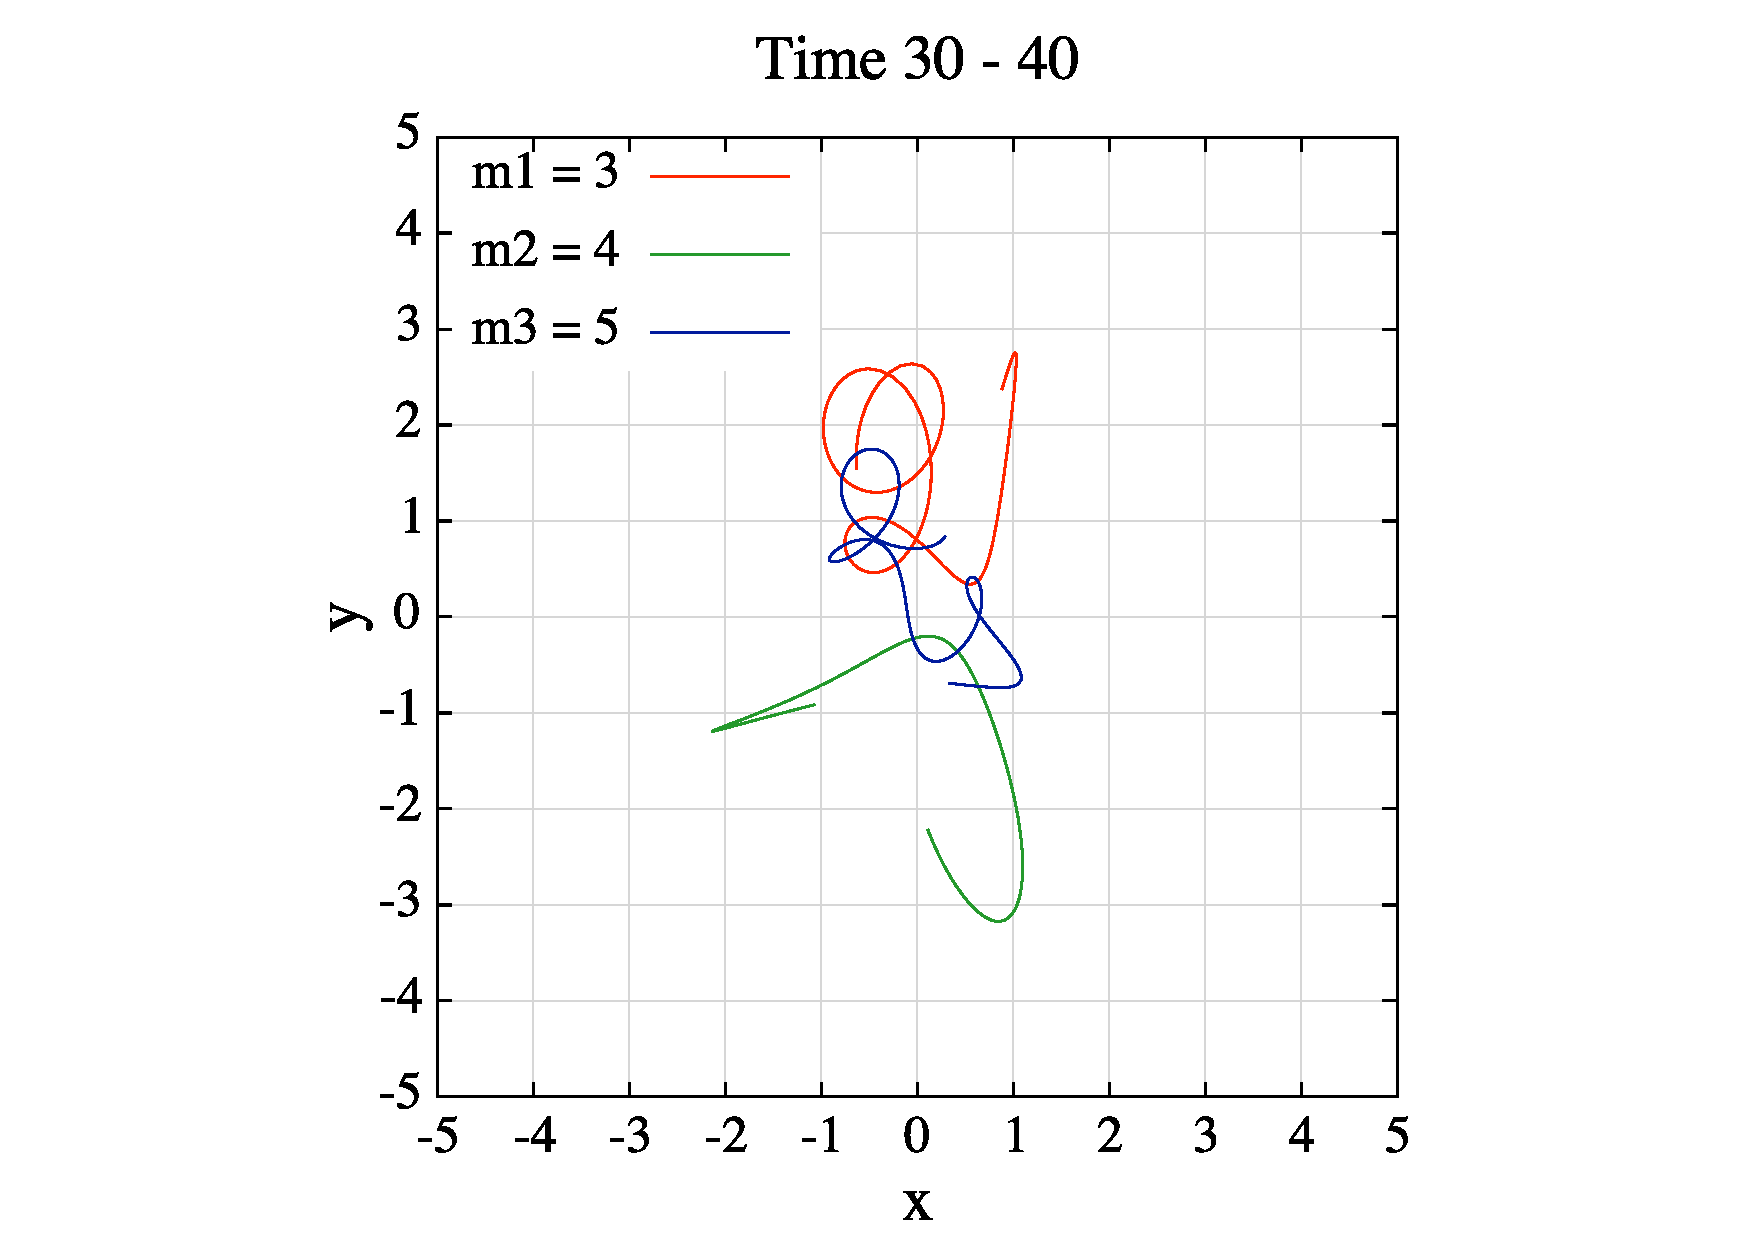
\includegraphics[width=8cm]{./image/pythagoras_orbit_30to40.pdf}
\end{minipage}\\
%
%左
\begin{minipage}[t]{0.45\hsize}
\centering
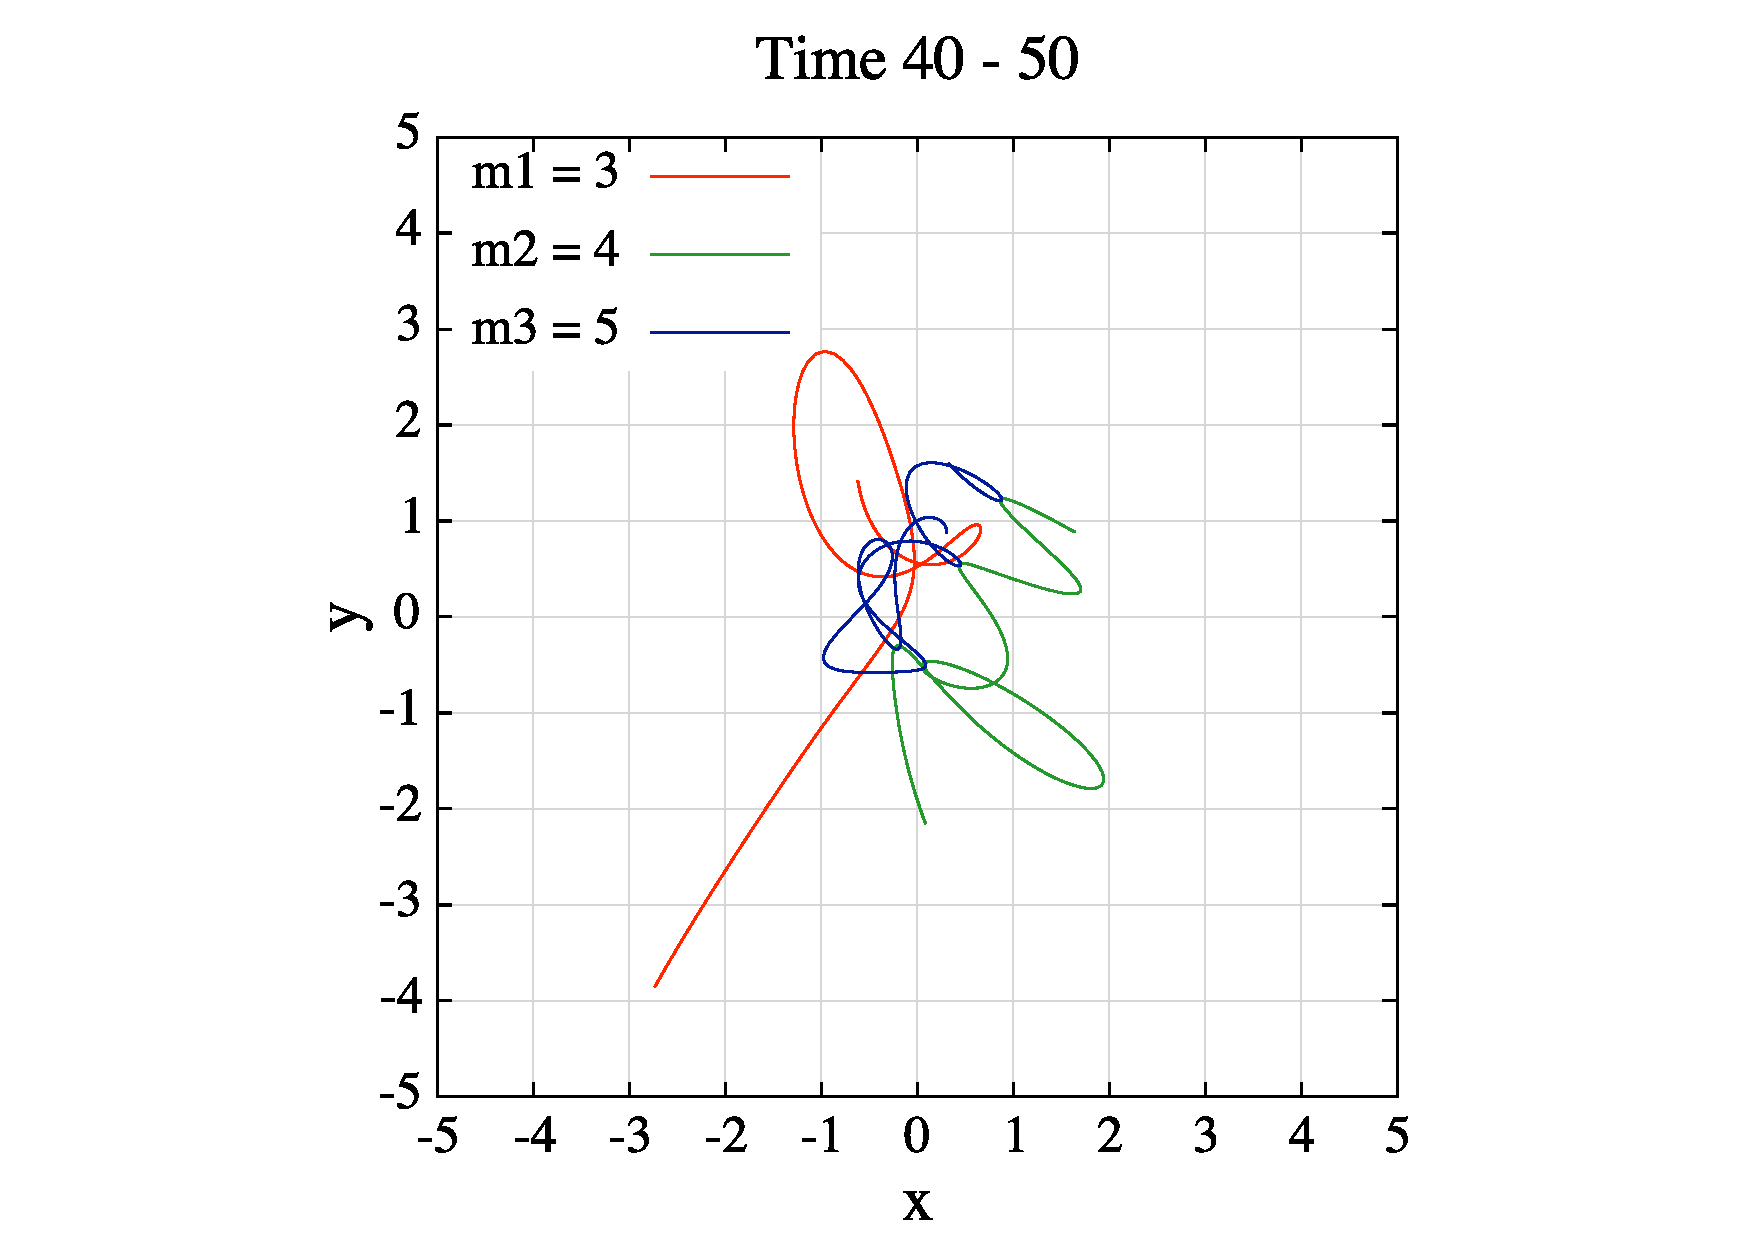
\includegraphics[width=8cm]{./image/pythagoras_orbit_40to50.pdf}
\end{minipage} &
%調整
\begin{minipage}[t]{0.1\hsize}
\end{minipage} &
%右
\begin{minipage}[t]{0.45\hsize}
\centering
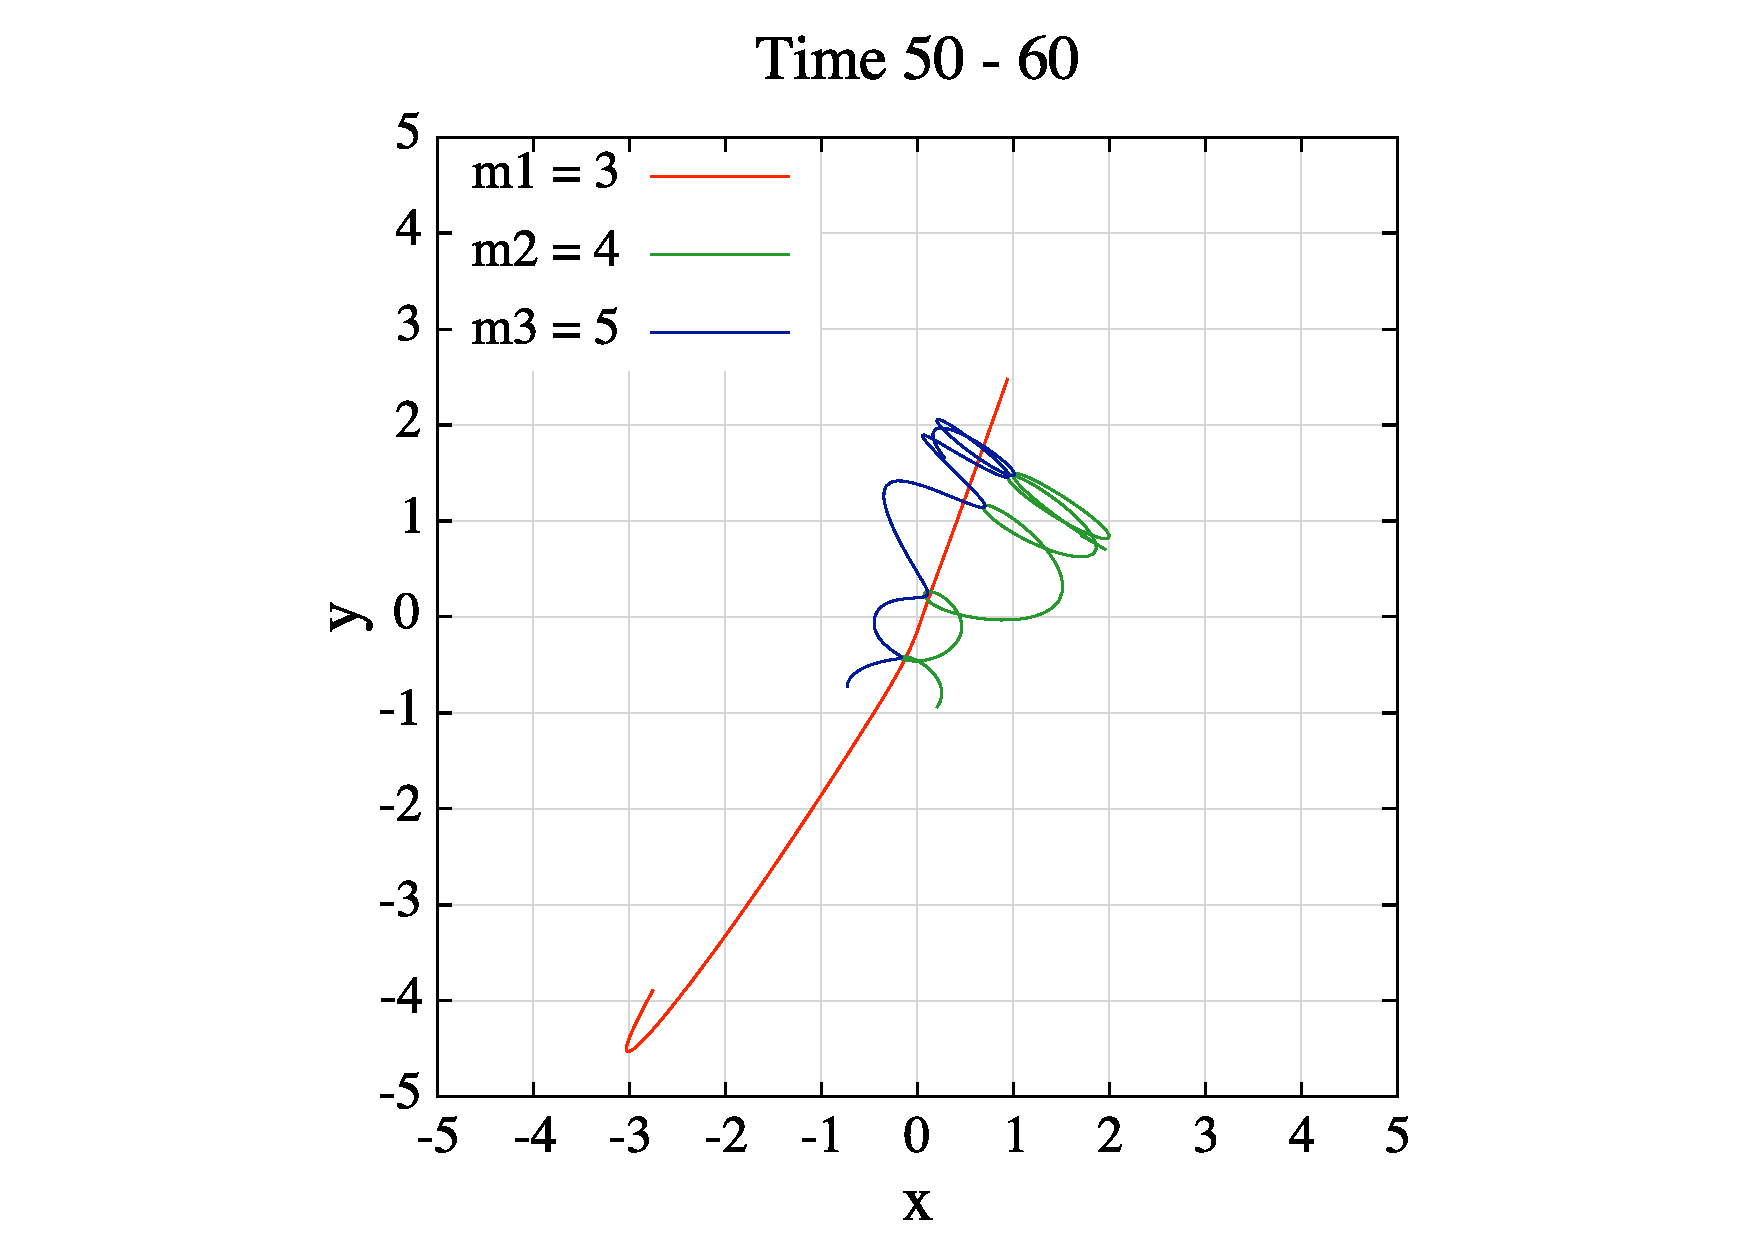
\includegraphics[width=8cm]{./image/pythagoras_orbit_50to60.pdf}
\end{minipage}\\
%
\begin{minipage}[t]{0.45\hsize}
\centering
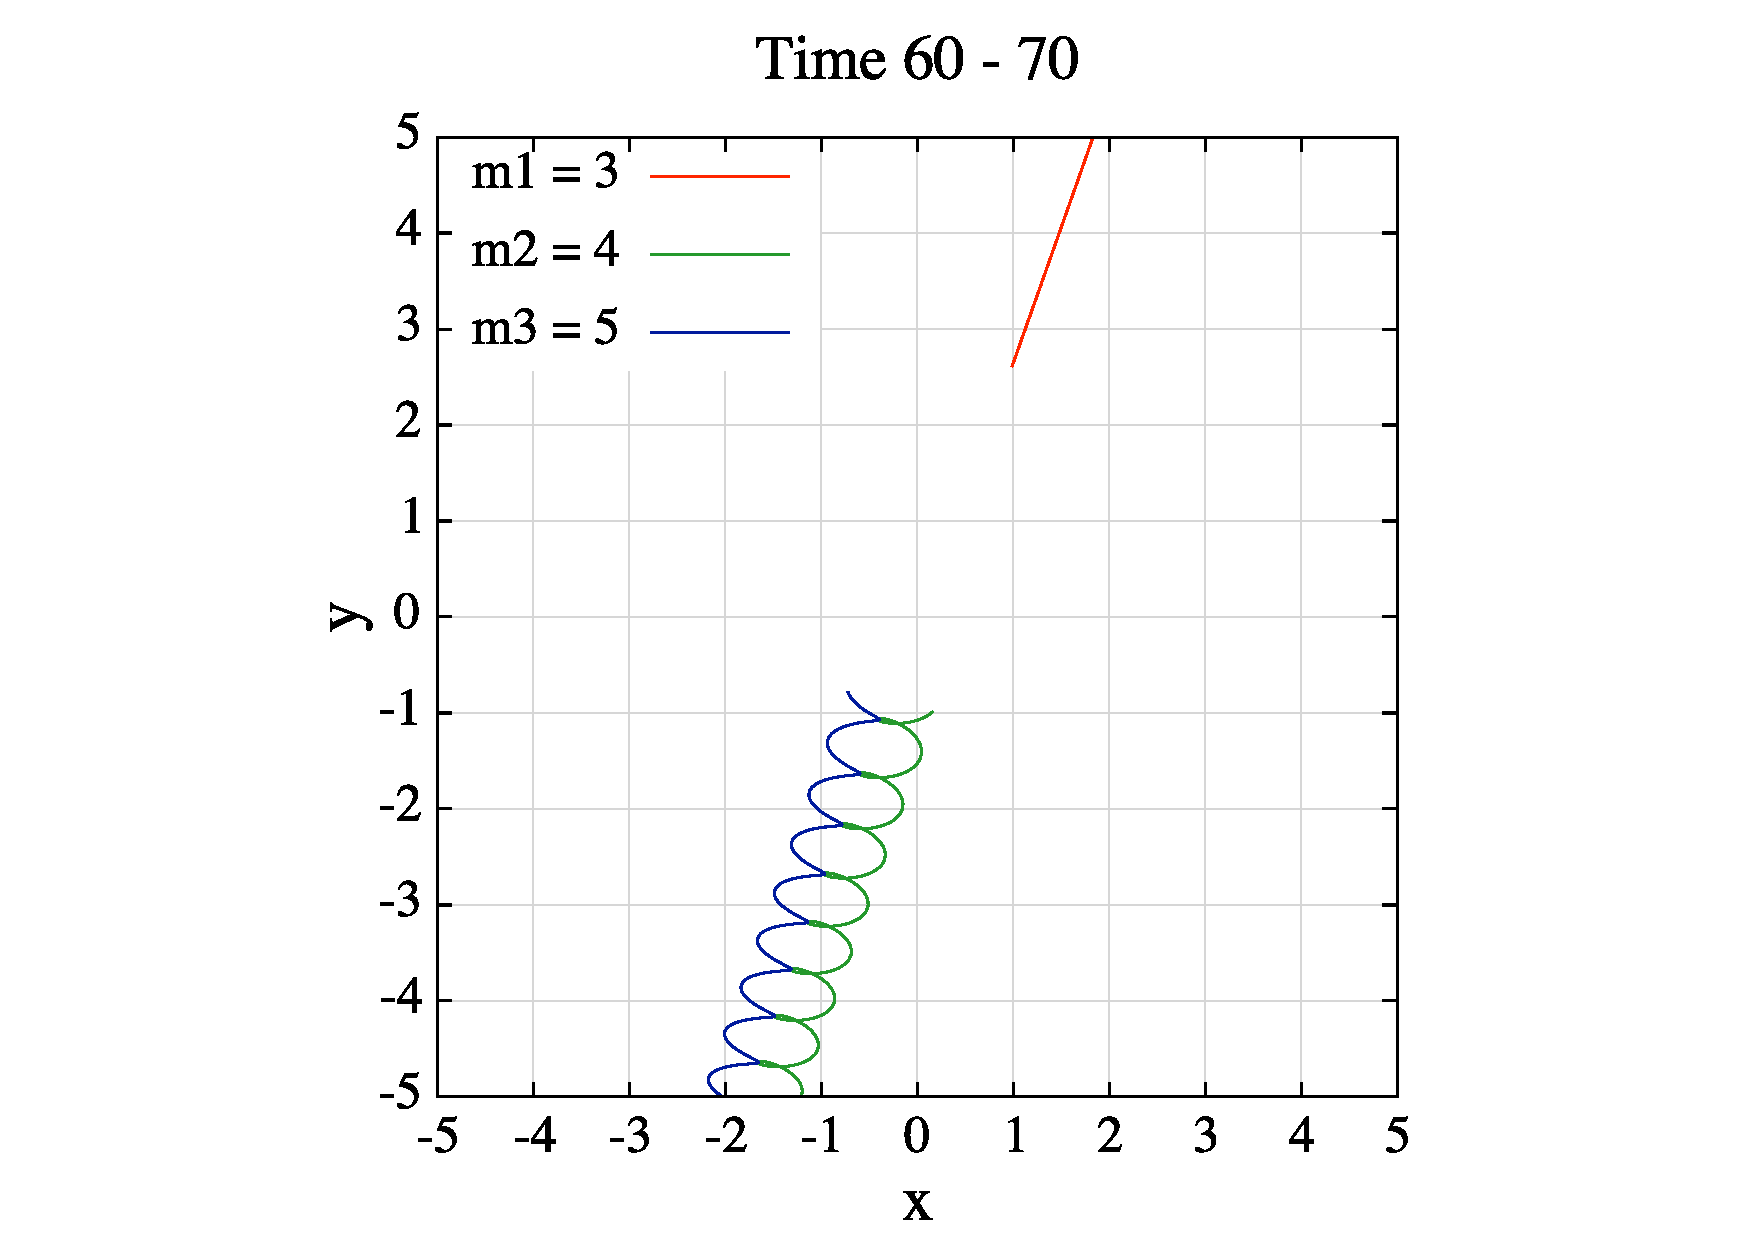
\includegraphics[width=8cm]{./image/pythagoras_orbit_60to70.pdf}
\end{minipage}
\end{tabular}
\caption{$t = 10$ごとの各質点の軌道.$t = 15.83$ 付近で質点 $m_2$ と質点 $m_3$ が最も接近し,$t = 60$ を超えたあたりからはその2つの質点が連星系をなして質点 $m_1$ と離れていく.\label{fig:pythagoras_orbit}}
\end{figure}

また,3つの質点の全エネルギーの相対誤差を計算し,その時間変化をプロットしたものが図\ref{fig:pythagoras_E_error}である.ここで,相対誤差はその時間での値と初期値の差を初期値の絶対値で割ったものとして計算している(負もとりうる).さらに,$t = 15.83$ 付近でのエネルギー相対誤差を詳しく見るために拡大したものが図\ref{fig:pythagoras_E_error_detail}である.
\begin{figure}[H]
\centering
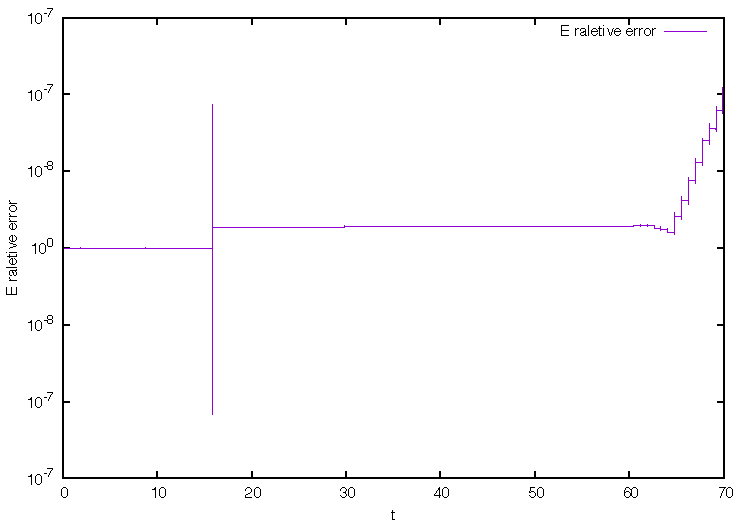
\includegraphics[width=8cm]{./image/pythagoras_E_error.pdf}
\caption{全エネルギーの相対誤差の時間変化.\label{fig:pythagoras_E_error}}
\end{figure}

\begin{figure}[H]
\centering
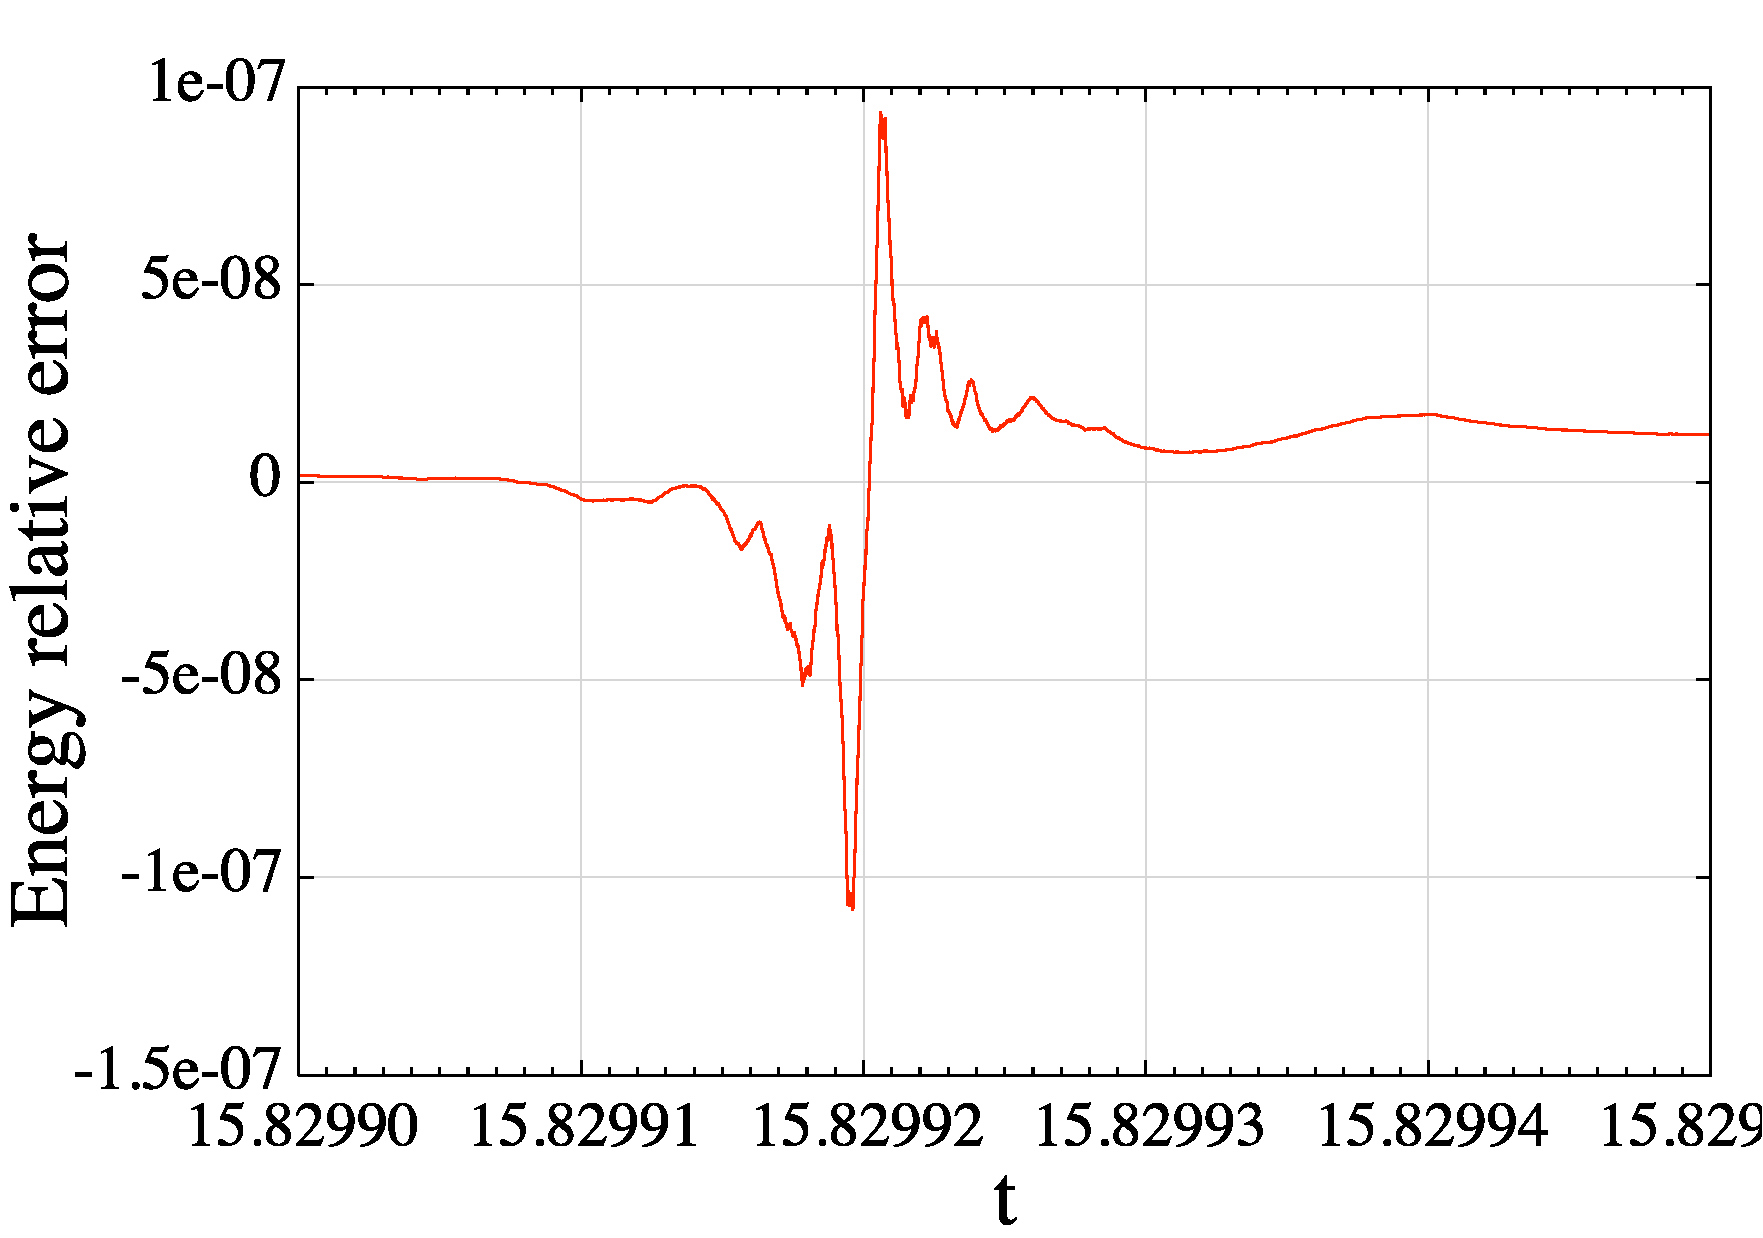
\includegraphics[width=8cm]{./image/pythagoras_E_error_detail.pdf}
\caption{全エネルギーの相対誤差の時間変化のうち,$t = 15.83$ 付近の最接近を拡大.\label{fig:pythagoras_E_error_detail}}
\end{figure}

\section{惑星移動に伴う小天体の軌道変化の数値計算}
先行研究で使われた惑星移動モデル\cite{Malhotra}\cite{Minton}を模擬し,木星を内側へ $0.2 {\rm AU}$,土星を外側へ $0.8 {\rm AU}$,天王星を外側へ $3.0 {\rm AU}$,海王星を外側へ $7.0 {\rm AU}$ 移動させたときの,惑星や小天体の軌道要素の時間変化を数値計算によって求めた.

この計算では,タイムステップは individual timestep を用い,$\eta = 0.05$,softning parameter $\epsilon = 0$,iteration は3回とした.

惑星の移動のさせ方は,軌道長半径が $\tau$ 程度の時間をかけて,
\begin{equation}
a (t) = a_f - \Delta a \exp \left( - \frac{t}{\tau} \right) \label{eq:a(t)}
\end{equation}
とゆっくり変化するように,手で加える加速度を
\begin{equation}
\Delta \ddot{\bm r} = \frac{\hat{{\bm v}}}{\tau} \left[ \sqrt{\frac{G M_{\odot}}{a_f}} - \sqrt{\frac{G M_{\odot}}{a_i}} \right] \exp \left(- \frac{t}{\tau} \right) \label{eq:delta_rddot}
\end{equation}
のように与えた\cite{Malhotra}.ここで,$\hat{{\bm v}}$ は速度方向の単位ベクトル,$\Delta a$ は移動距離,$a_f$ は現在の軌道長半径,$a_i = a_f - \Delta a$ は初期の軌道長半径である.

この加速度を与えたときの軌道長半径の時間変化について詳しく計算する.円軌道 $e = 0$を仮定すると,円柱座標系において速度方向は $\theta$ 方向と平行であるため,上で与える加速度のような微小摂動力は $d {\bm F} = \bar{T} \hat{\bm \theta}$ とおける.ガウスの惑星方程式を用いると,
\begin{equation}
\frac{d a}{d t} = 2 \frac{a^{3/2}}{\sqrt{G M_{\odot}}} \bar{T}, \quad \bar{T} = \frac{1}{\tau} \left[ \sqrt{\frac{G M_{\odot}}{a_f}} - \sqrt{\frac{G M_{\odot}}{a_i}} \right] \exp \left(- \frac{t}{\tau} \right)
\end{equation}
両辺積分して整理すると,
\begin{equation}
a (t) = a_f \left[ 1 - \left( 1 - \frac{1}{\sqrt{1 - \Delta a/ a_f}} \right) \exp \left( - \frac{t}{\tau} \right) \right]^{-2} \label{eq:a(t)_new}
\end{equation}
$\Delta a \ll a_f$ である場合,$\Delta a/ a_f$ の1次までの近似を行うと,
\begin{equation}
\begin{split}
a (t) & \approx a_f \left[ 1 + 2 \left( 1 - \frac{1}{\sqrt{1 - \Delta a/ a_f}} \right) \exp \left( - \frac{t}{\tau} \right) \right] \\
& \approx a_f \left[ 1 - \frac{\Delta a}{a_f} \exp \left( - \frac{t}{\tau} \right) \right] \\
& = a_f - \Delta a \exp \left( - \frac{t}{\tau} \right)
\end{split}
\label{eq:a(t)_approx}
\end{equation}
したがって,式(\ref{eq:delta_rddot})のような加速度の与え方は,$\Delta a \ll a_f$ である場合にのみ正しく,実際には $\Delta a/ a_f$ は木星 : $0.2 / 5.2 = 0.038$,土星 : $0.8 / 9.5 = 0.084$,天王星 : $3.0 /19.2 = 0.156$,海王星 : $7.0 / 30.1 = 0.233$ であるため,式(\ref{eq:a(t)})のような軌道長半径の時間変化を厳密には実現できていない.しかし,本研究では惑星移動の時間 $\tau$ の正確さよりも,惑星やテスト粒子の軌道要素の変化を正確に計算することに重きを置いているため,また初期値を決めたら後は時間にのみ依存する表式がシンプルであるため,式(\ref{eq:delta_rddot})を用いた.

惑星移動の時間は $\tau = 0.5 {\rm Myr}$ とし,惑星の質量は $5 {\rm Myr}$ の時間をかけて線形的に増加させた\cite{Minton}.

太陽は惑星との重力相互作用で動くはずであるが,太陽に比べて惑星の質量が十分小さいとし,太陽は原点に固定されているものと考え,太陽重力は外場として扱った.

テスト粒子が4つのうちいずれかの惑星のヒル圏内に入った場合や,離心率が1を超えて双曲線軌道になる場合には,その粒子は計算をやめ,プログラム中でループから外すようにしている.このようにすることで,タイムステップが小さくなりすぎて計算が遅くなることを防ぎ,また小惑星帯やカイパーベルトの小天体がどの程度減らされるのかを確認することができる.

惑星の軌道要素の初期値として,NASA Planetary Fact Sheets\footnote{\url{http://nssdc.gsfc.nasa.gov/planetary/planetfact.html}}の Mean Orbital Elements (J2000)の値を引用した.


\subsection{4つの巨大惑星の4体シミュレーション}
「重力相互作用」と「永年共鳴の位置の移動」を確認するため,まずは巨大惑星4つのみの4体計算を行った.
\subsubsection{重力相互作用}
比較のため,惑星を動かさない場合と動かした場合の2種類を計算した.以下の図は軌道要素の $5 {\rm Myr}$ 分の時間変化をプロットしたものである.

\begin{figure}[H]
\begin{tabular}{ccc}
%左
\begin{minipage}[t]{0.45\hsize}
\centering
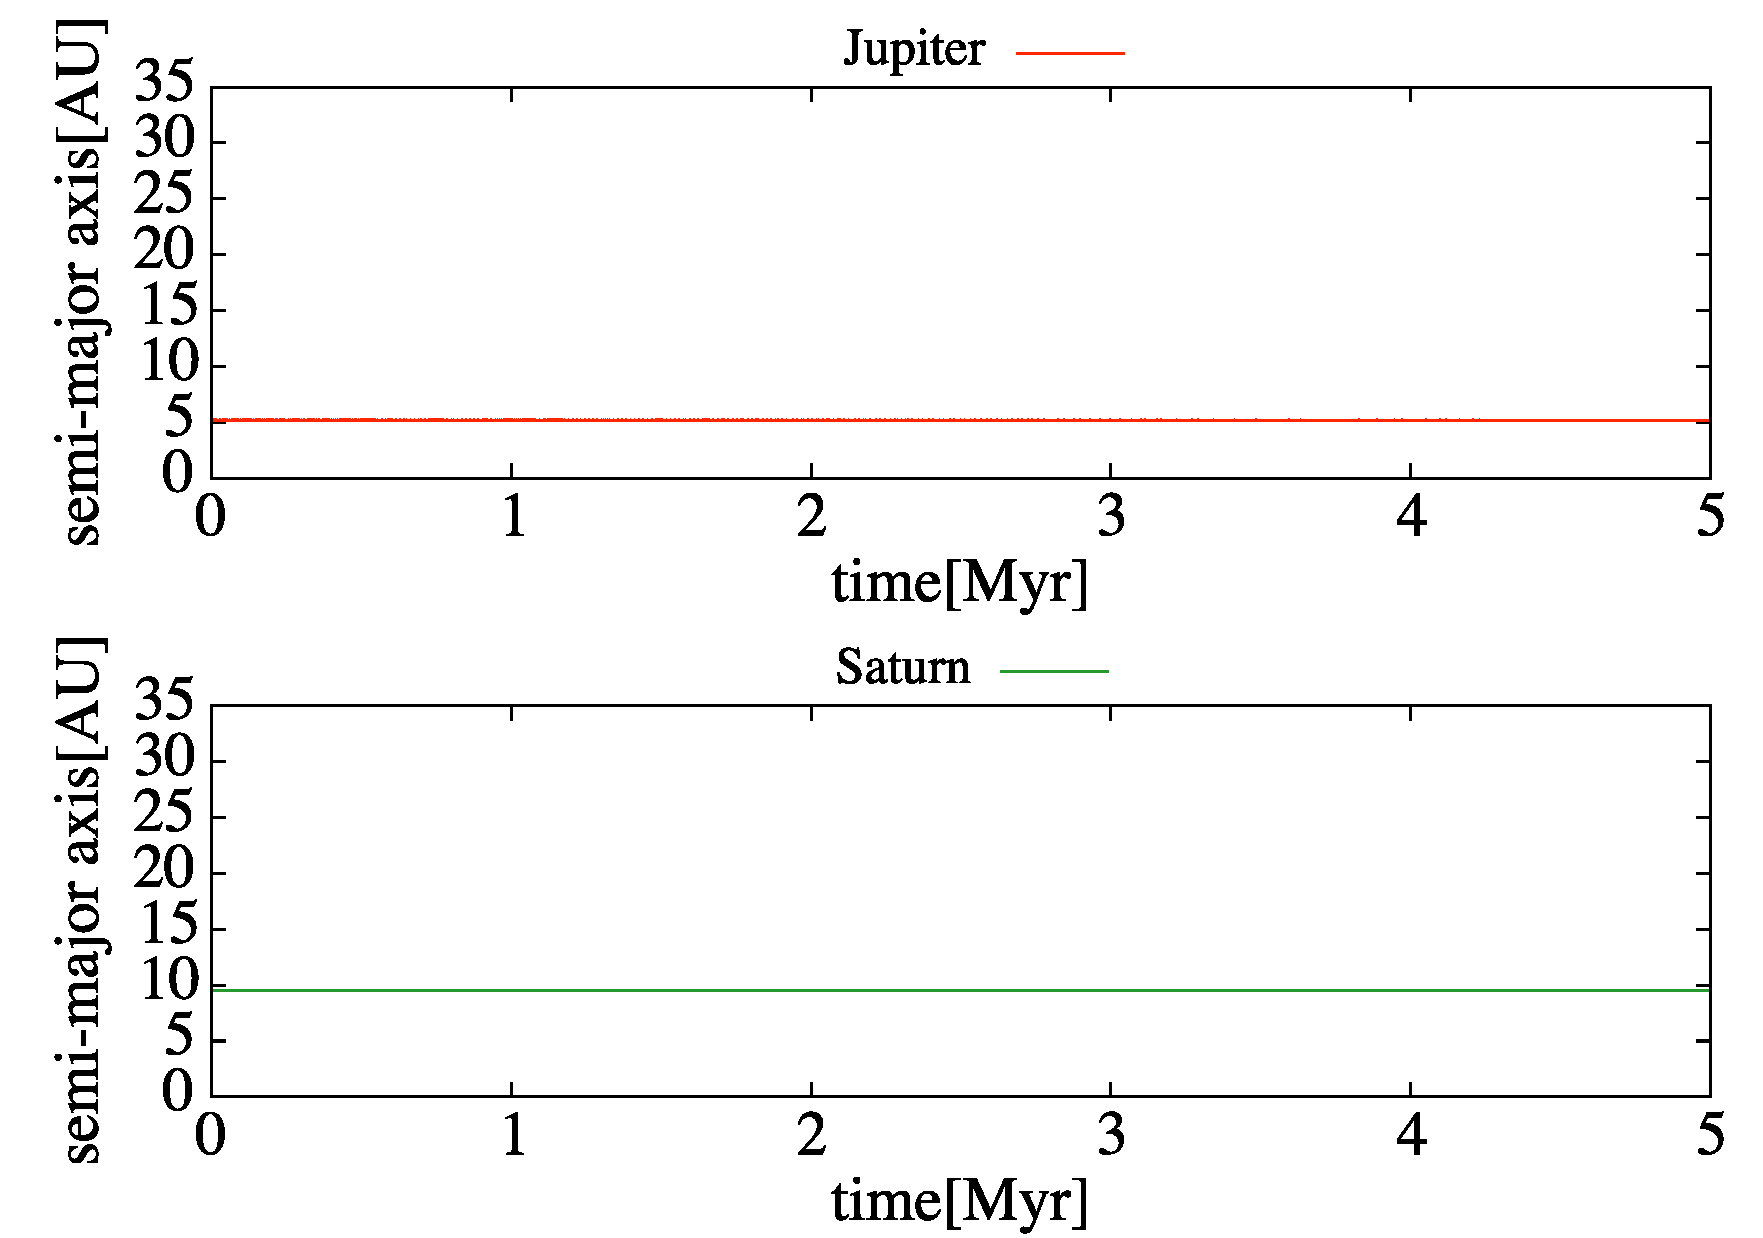
\includegraphics[width=8cm]{./image/NoMove_axis_5Myr_JUPSAT.pdf}
\end{minipage} &
%調整
\begin{minipage}[t]{0.1\hsize}
\end{minipage} &
%右
\begin{minipage}[t]{0.45\hsize}
\centering
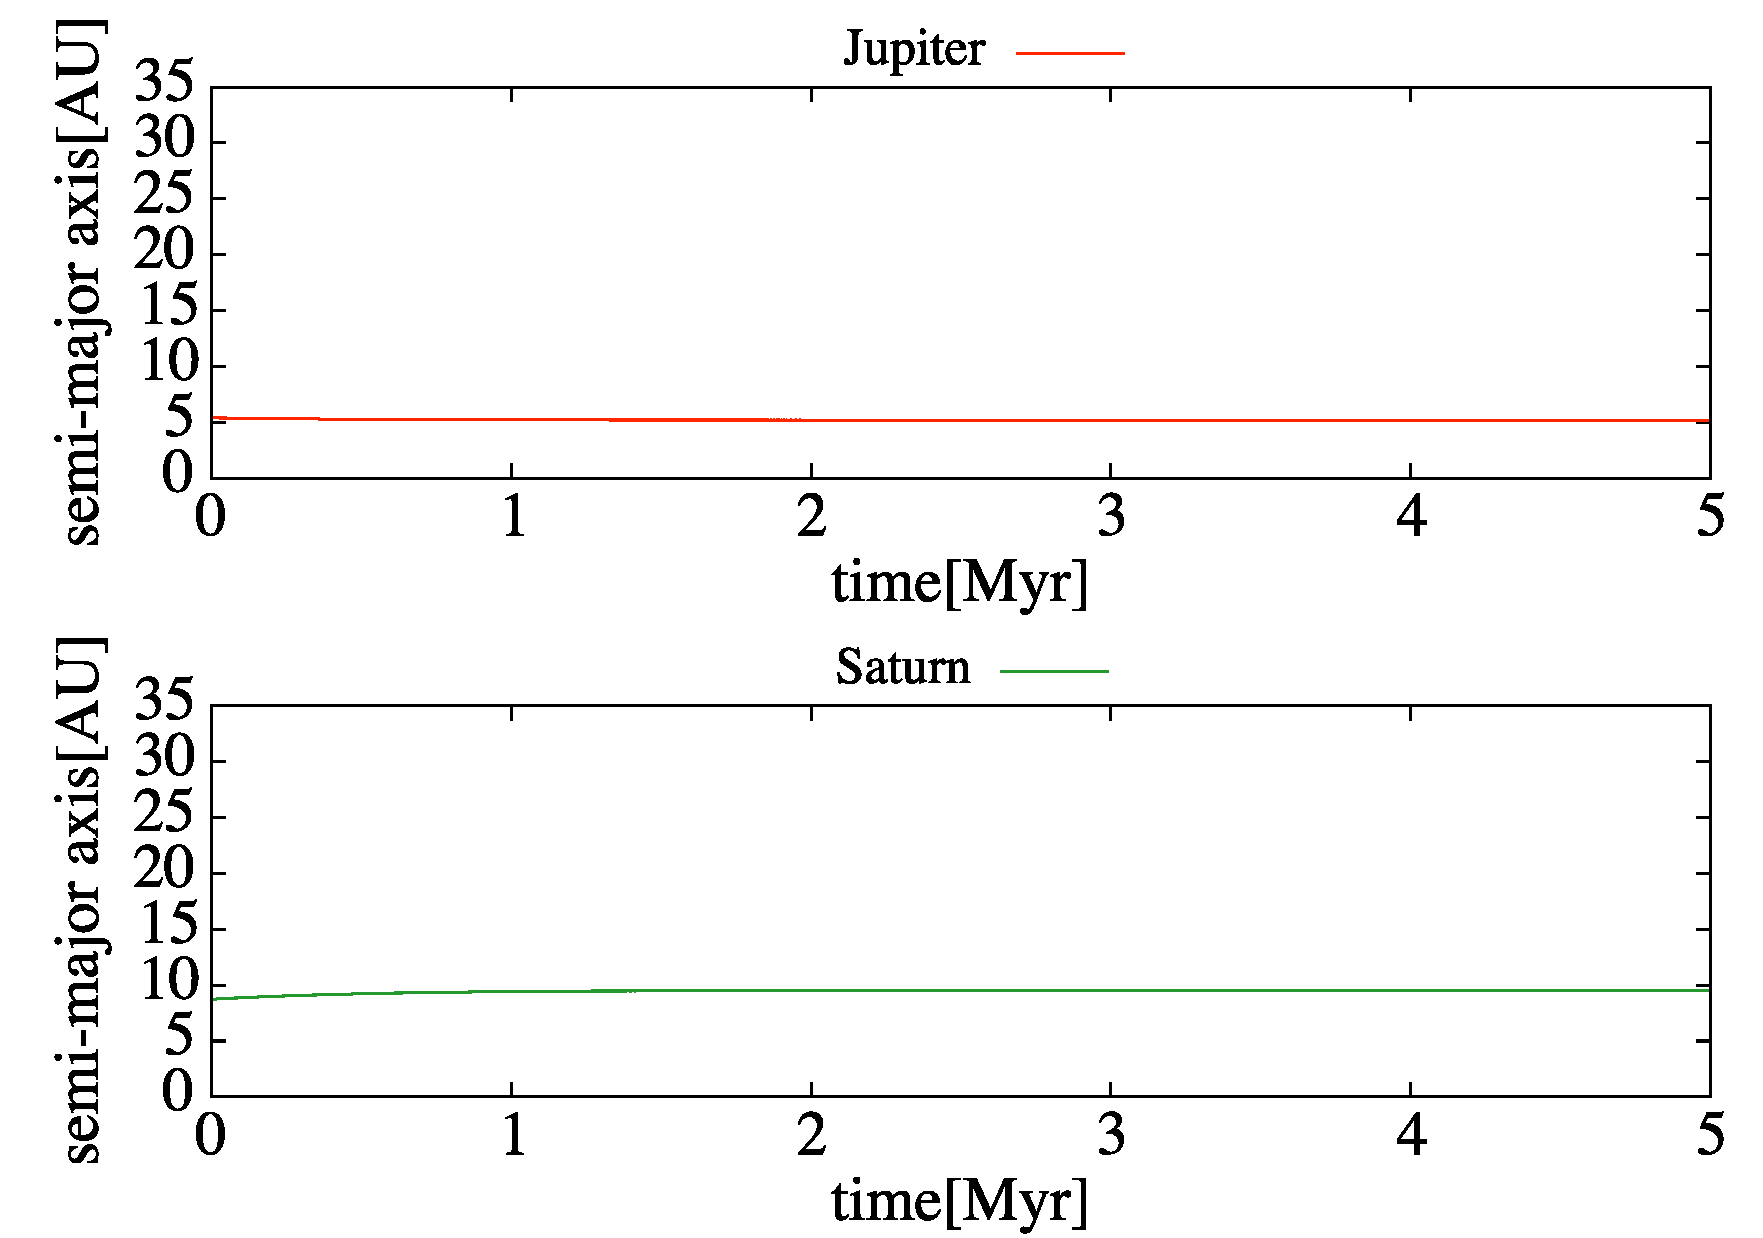
\includegraphics[width=8cm]{./image/Move500kyr_axis_5Myr_JUPSAT.pdf}
\end{minipage}\\
%左
\begin{minipage}[t]{0.45\hsize}
\centering
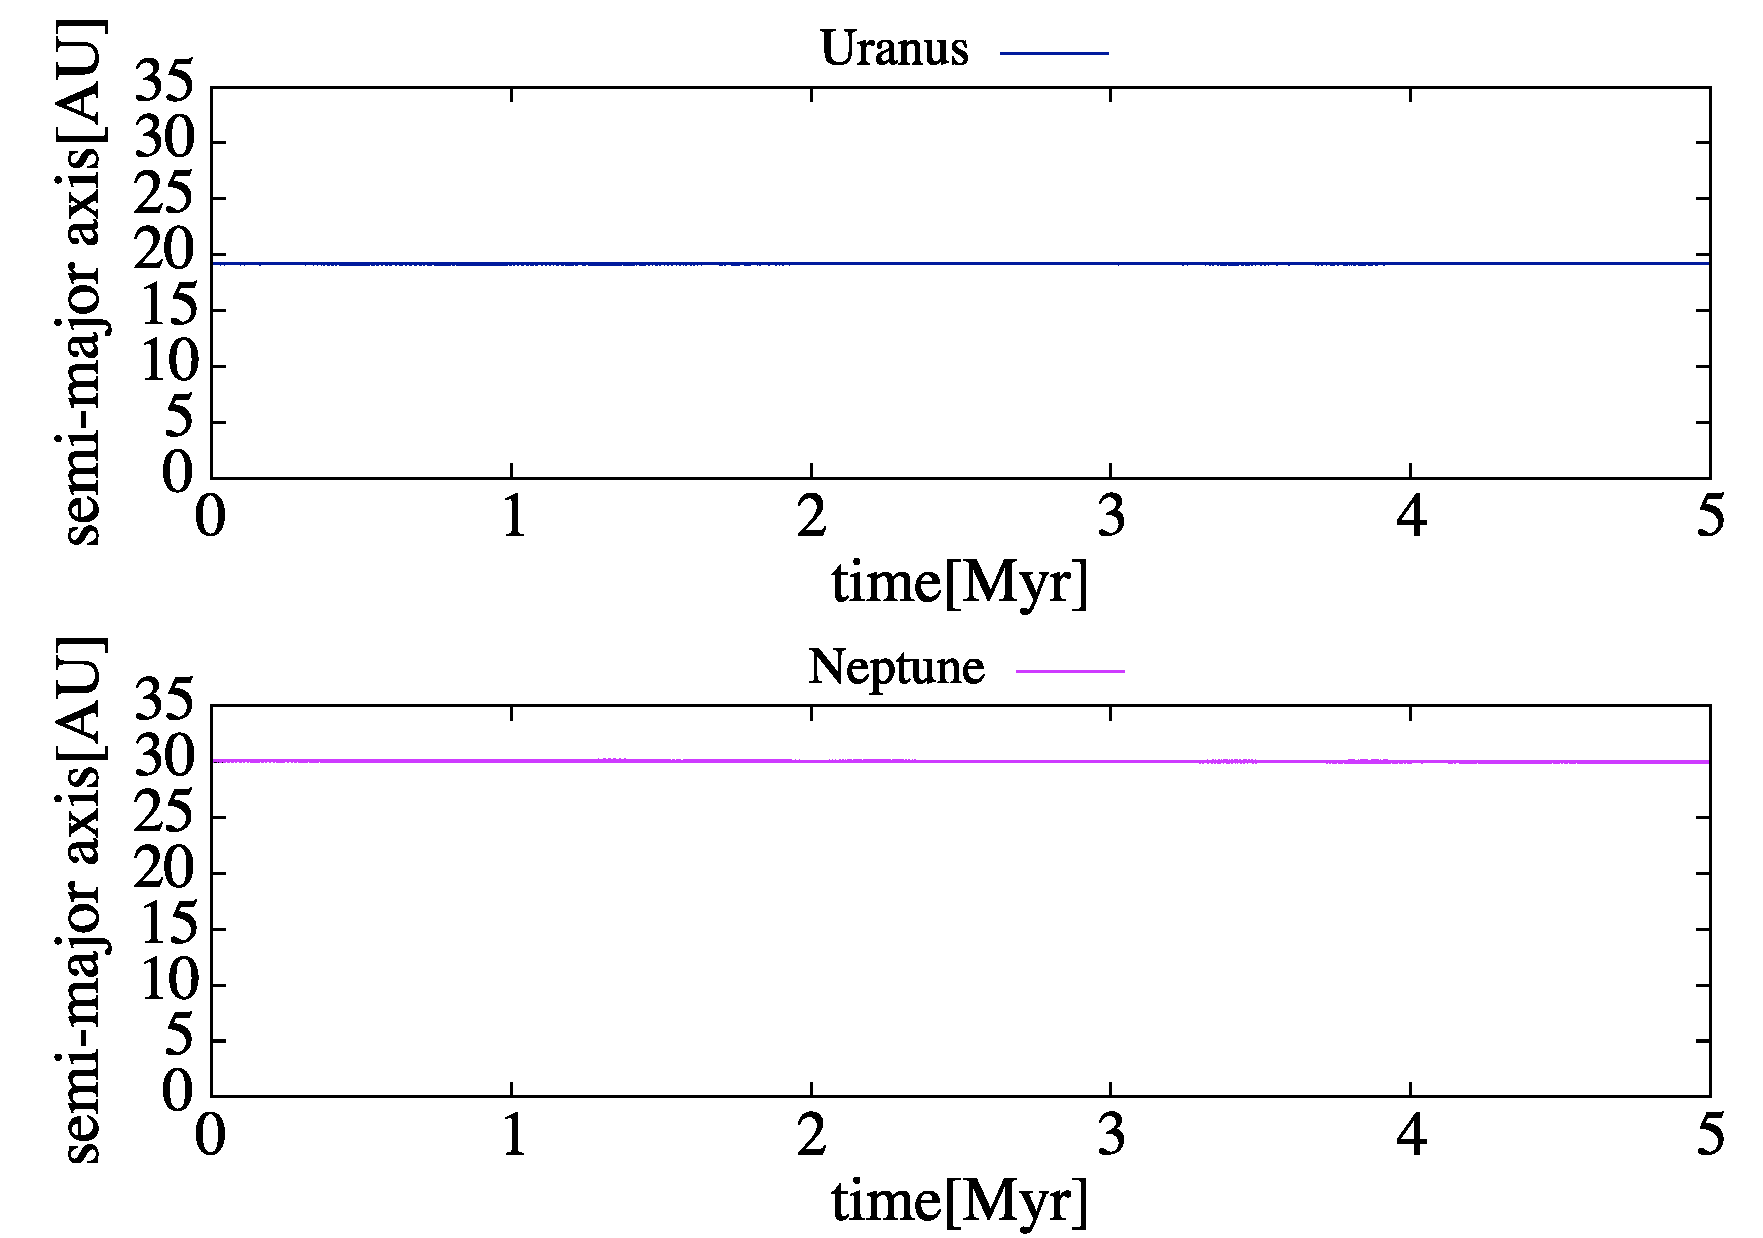
\includegraphics[width=8cm]{./image/NoMove_axis_5Myr_URANEP.pdf}
\end{minipage} &
%調整
\begin{minipage}[t]{0.1\hsize}
\end{minipage} &
%右
\begin{minipage}[t]{0.45\hsize}
\centering
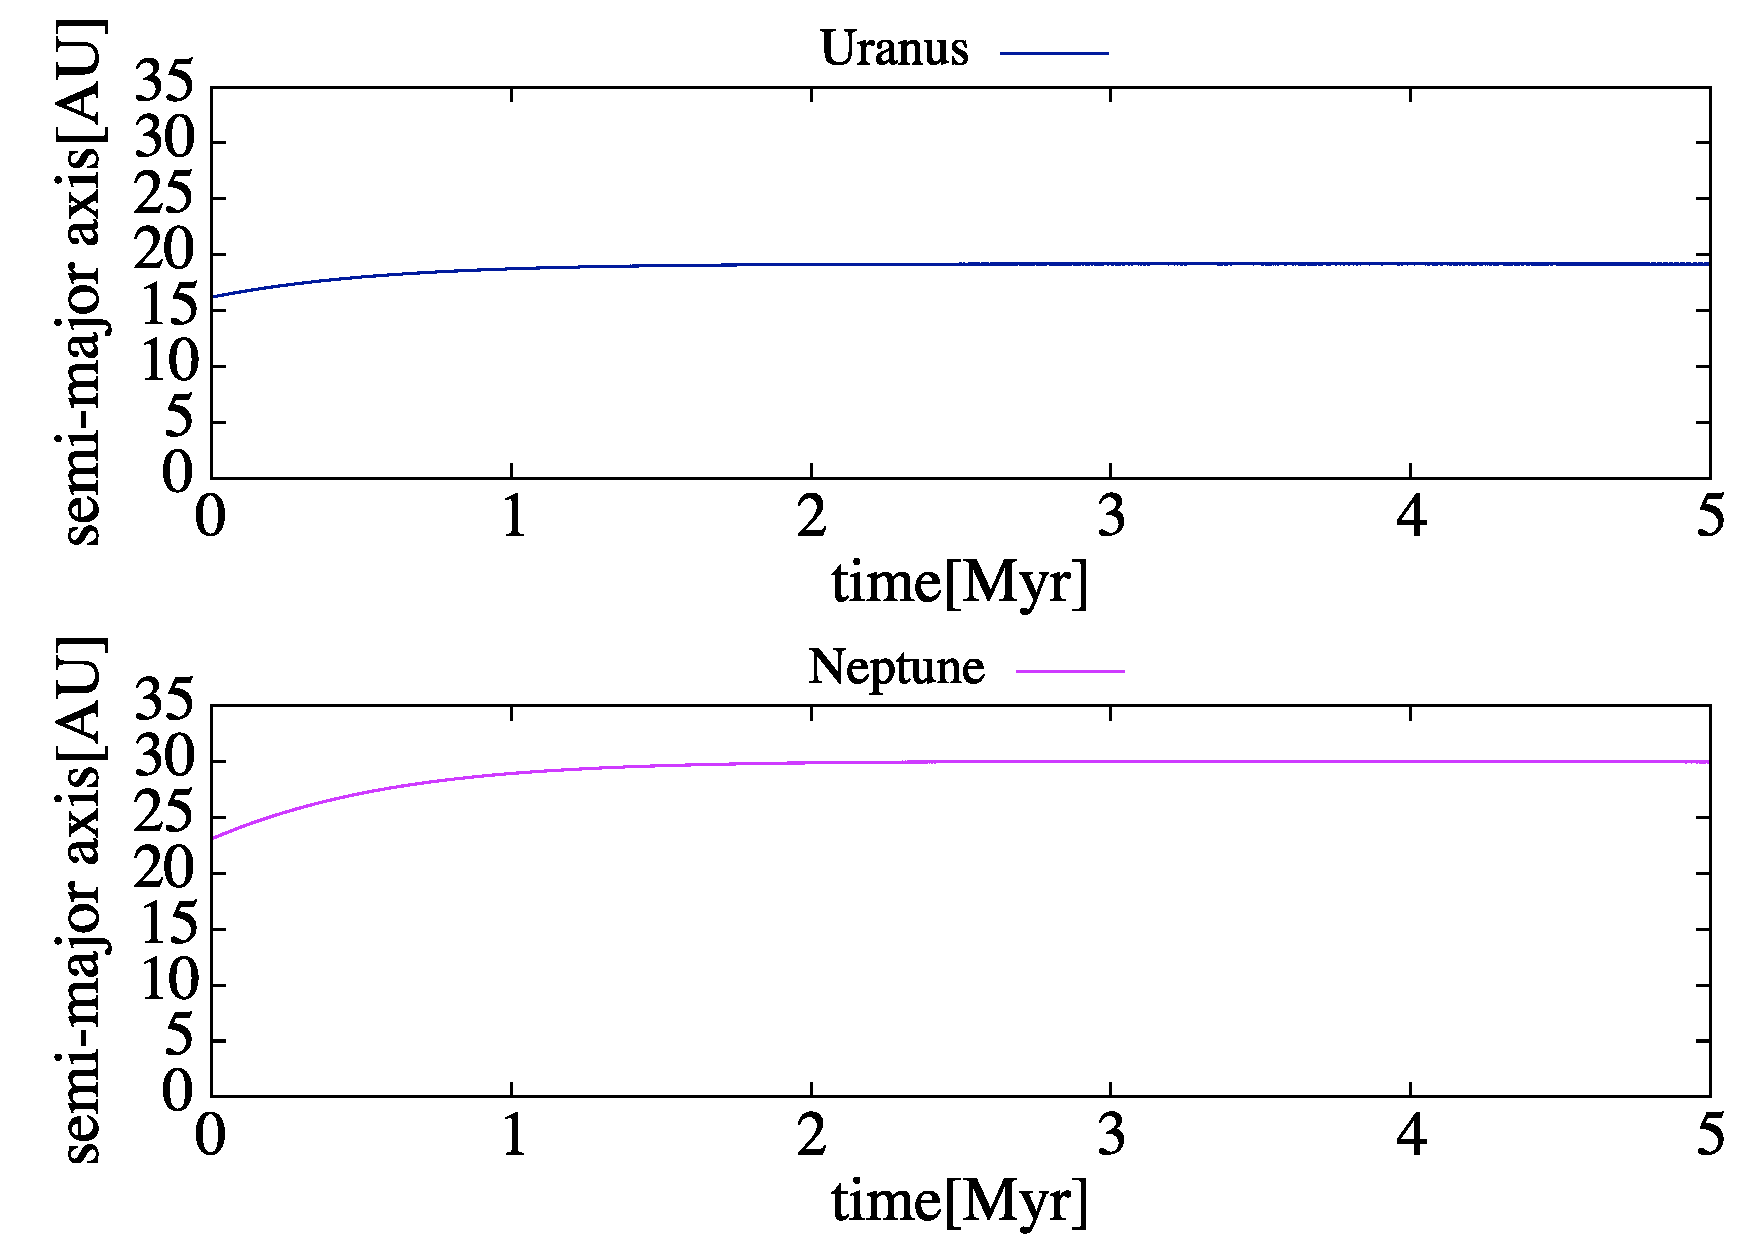
\includegraphics[width=8cm]{./image/Move500kyr_axis_5Myr_URANEP.pdf}
\end{minipage}
%
\end{tabular}
\caption{軌道長半径の変化.左が惑星移動なしの場合,右が惑星移動ありの場合,上から順に木星,土星,天王星,海王星である.\label{fig:axis}}
\end{figure}


\begin{figure}[H]
\begin{tabular}{ccc}
%左
\begin{minipage}[t]{0.45\hsize}
\centering
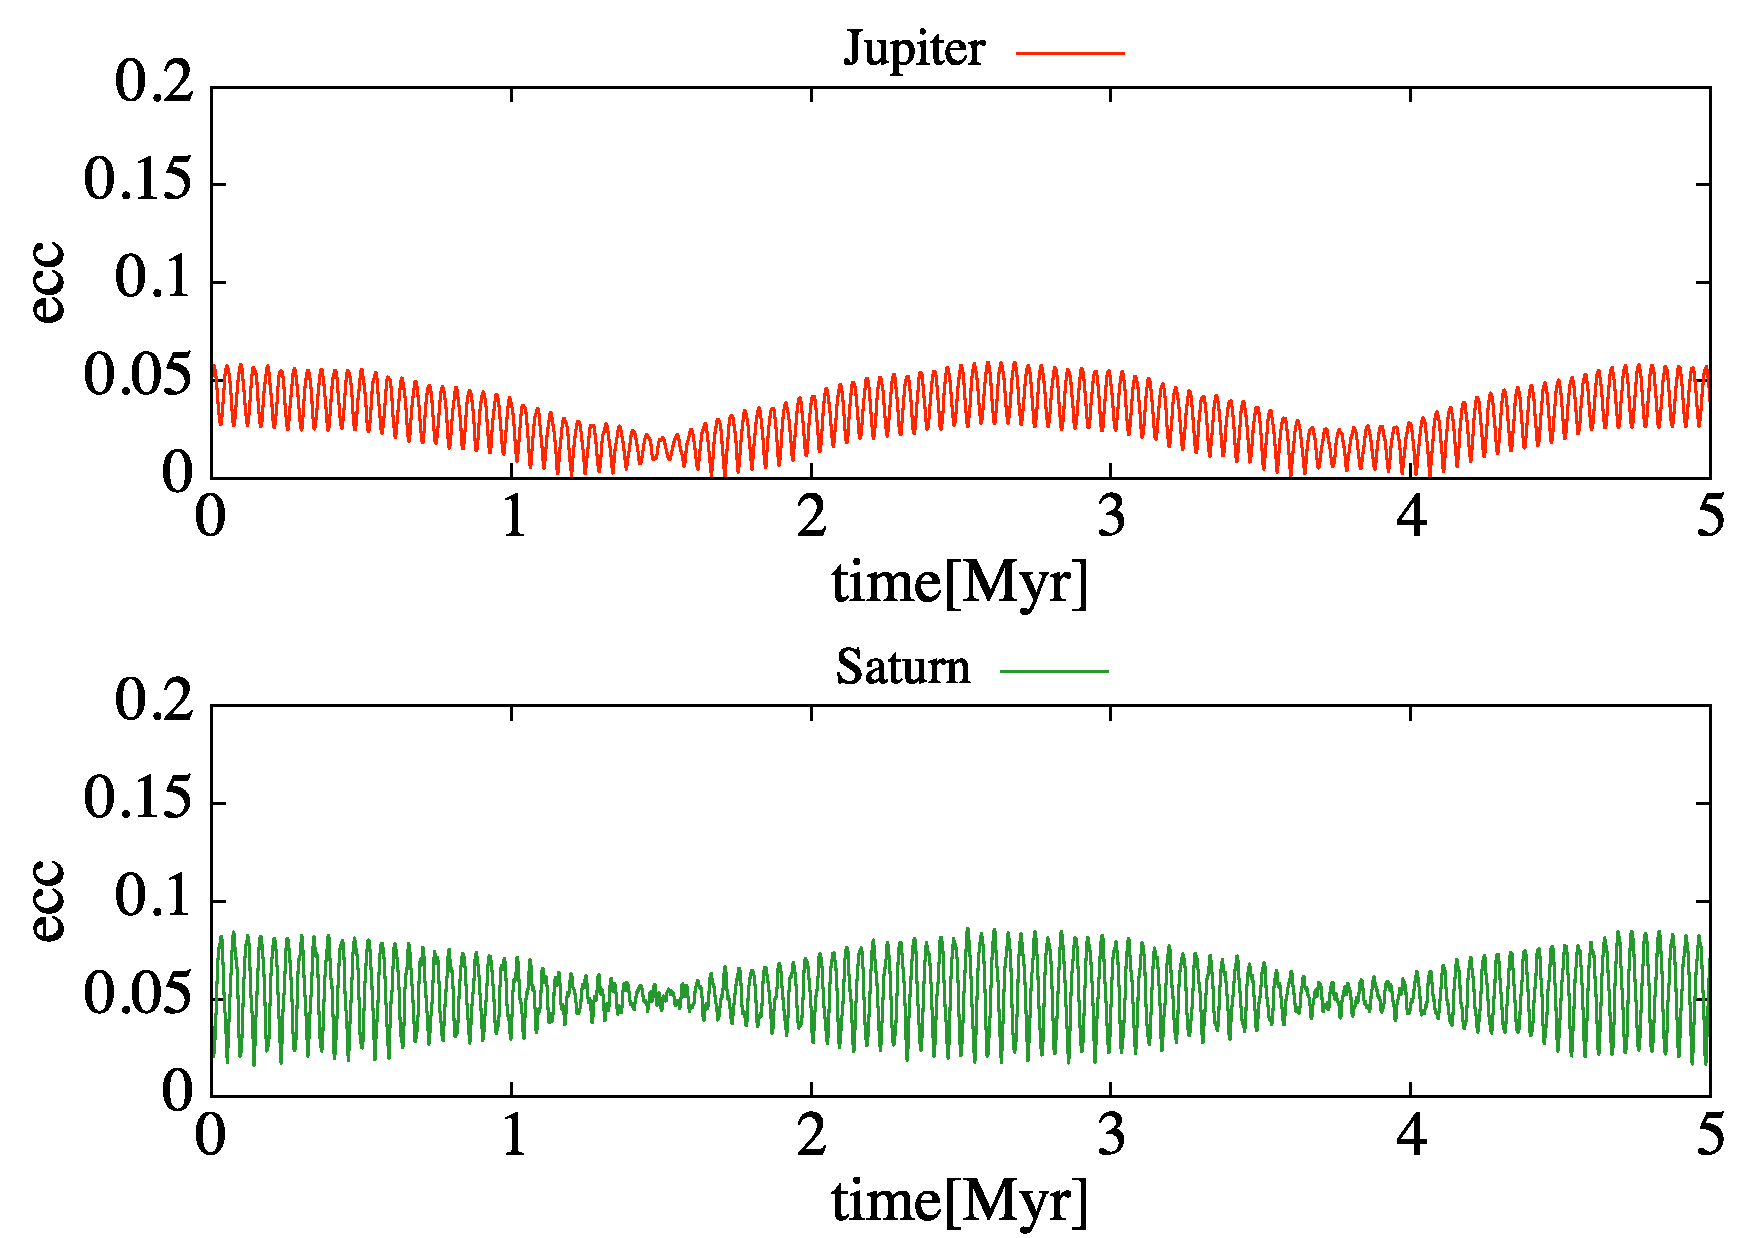
\includegraphics[width=8cm]{./image/NoMove_ecc_5Myr_JUPSAT.pdf}
\end{minipage} &
%調整
\begin{minipage}[t]{0.1\hsize}
\end{minipage} &
%右
\begin{minipage}[t]{0.45\hsize}
\centering
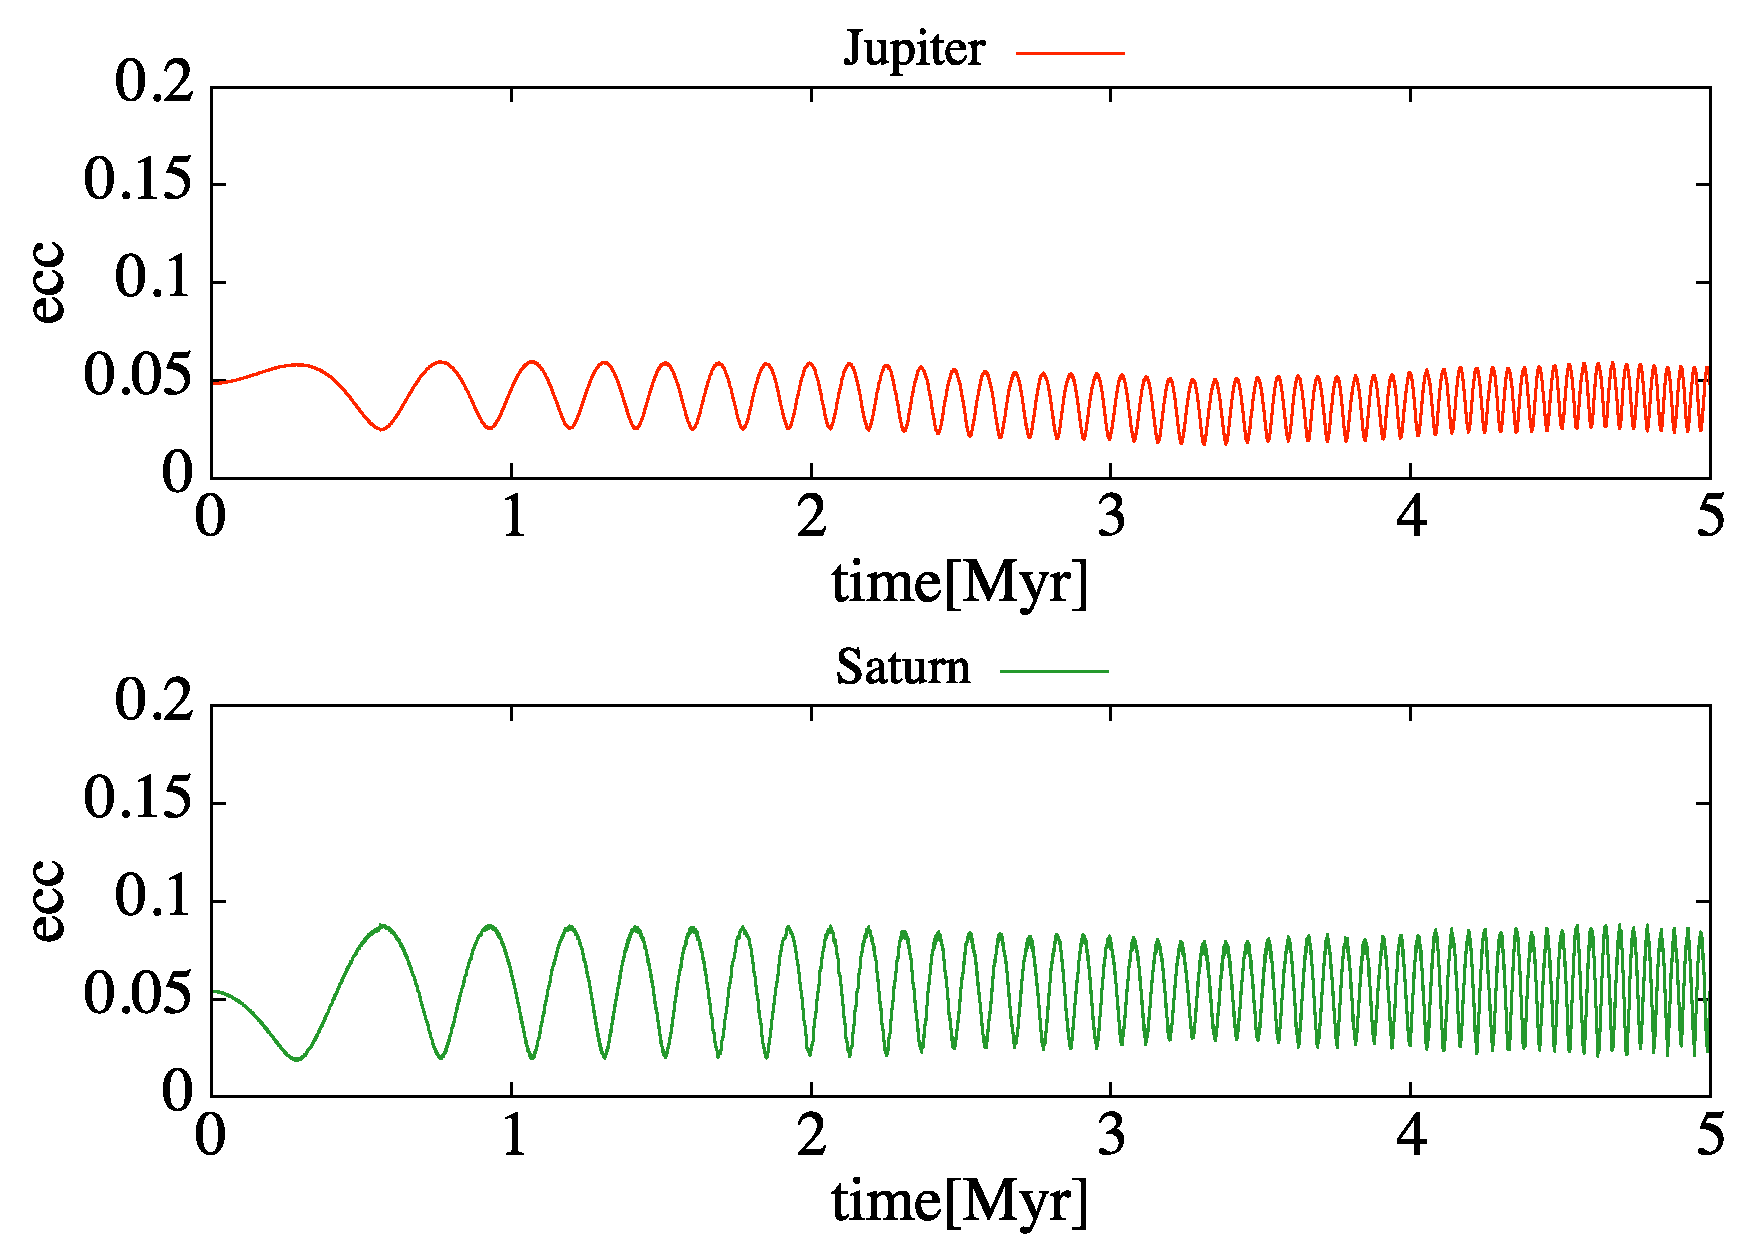
\includegraphics[width=8cm]{./image/Move500kyr_ecc_5Myr_JUPSAT.pdf}
\end{minipage}\\
%左
\begin{minipage}[t]{0.45\hsize}
\centering
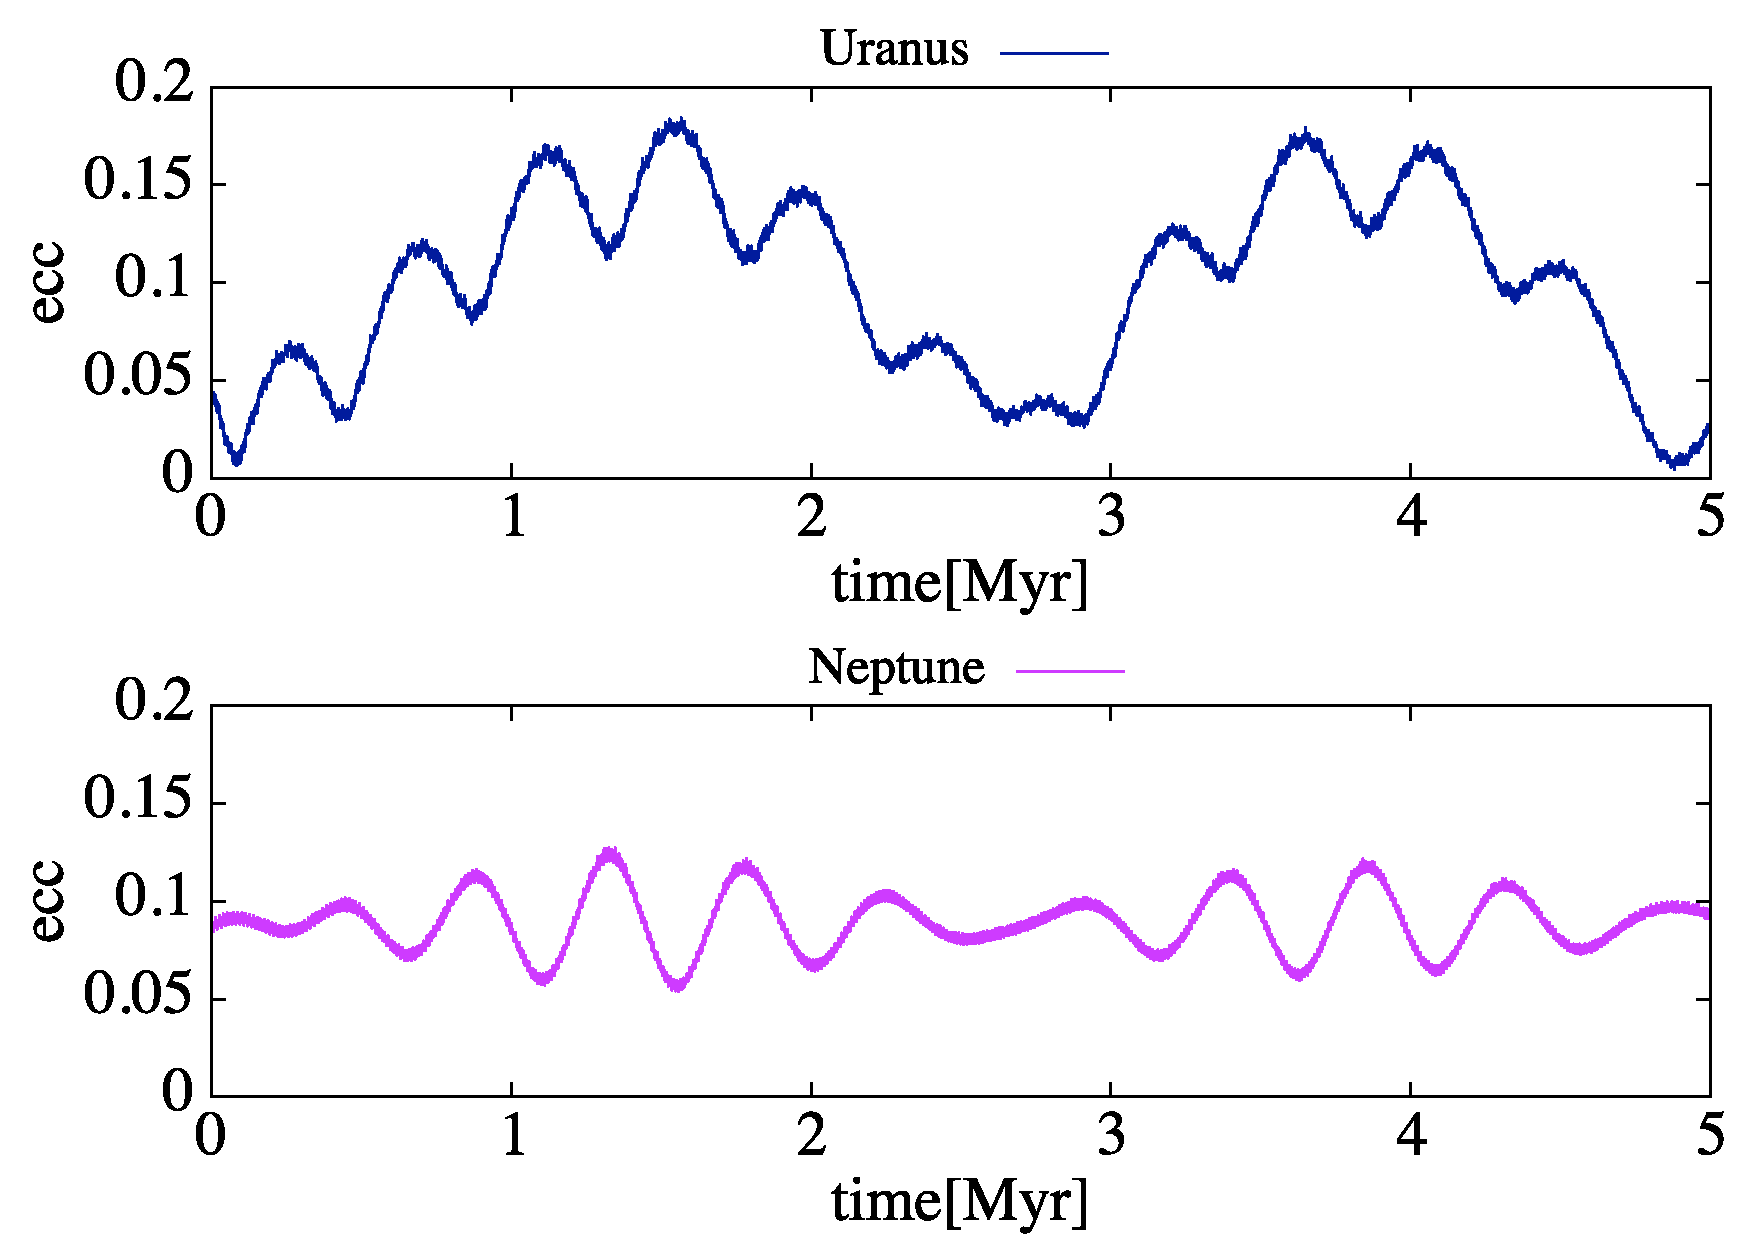
\includegraphics[width=8cm]{./image/NoMove_ecc_5Myr_URANEP.pdf}
\end{minipage} &
%調整
\begin{minipage}[t]{0.1\hsize}
\end{minipage} &
%右
\begin{minipage}[t]{0.45\hsize}
\centering
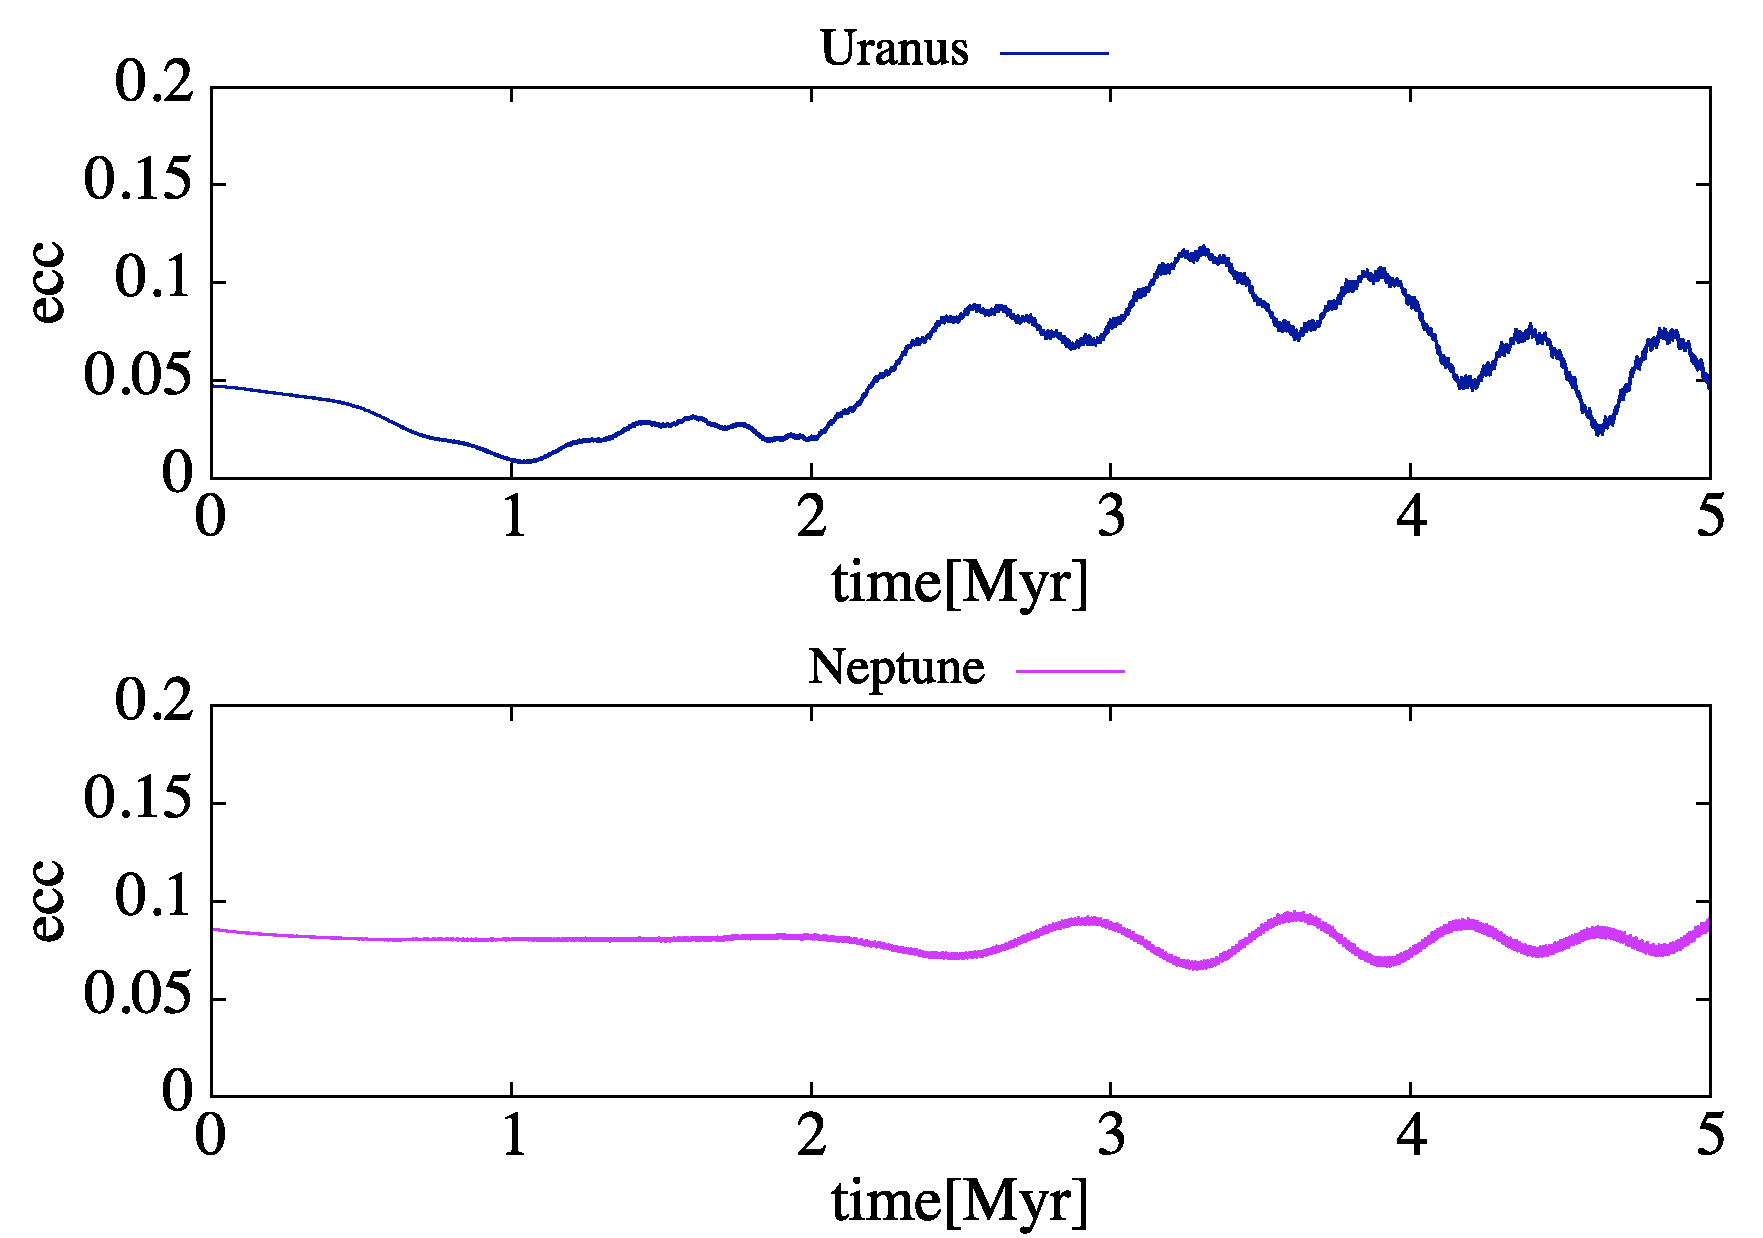
\includegraphics[width=8cm]{./image/Move500kyr_ecc_5Myr_URANEP.pdf}
\end{minipage}
%
\end{tabular}
\caption{離心率の変化.左が惑星移動なしの場合,右が惑星移動ありの場合,上から順に木星,土星,天王星,海王星である.\label{fig:ecc}}
\end{figure}


\begin{figure}[H]
\begin{tabular}{ccc}
%左
\begin{minipage}[t]{0.45\hsize}
\centering
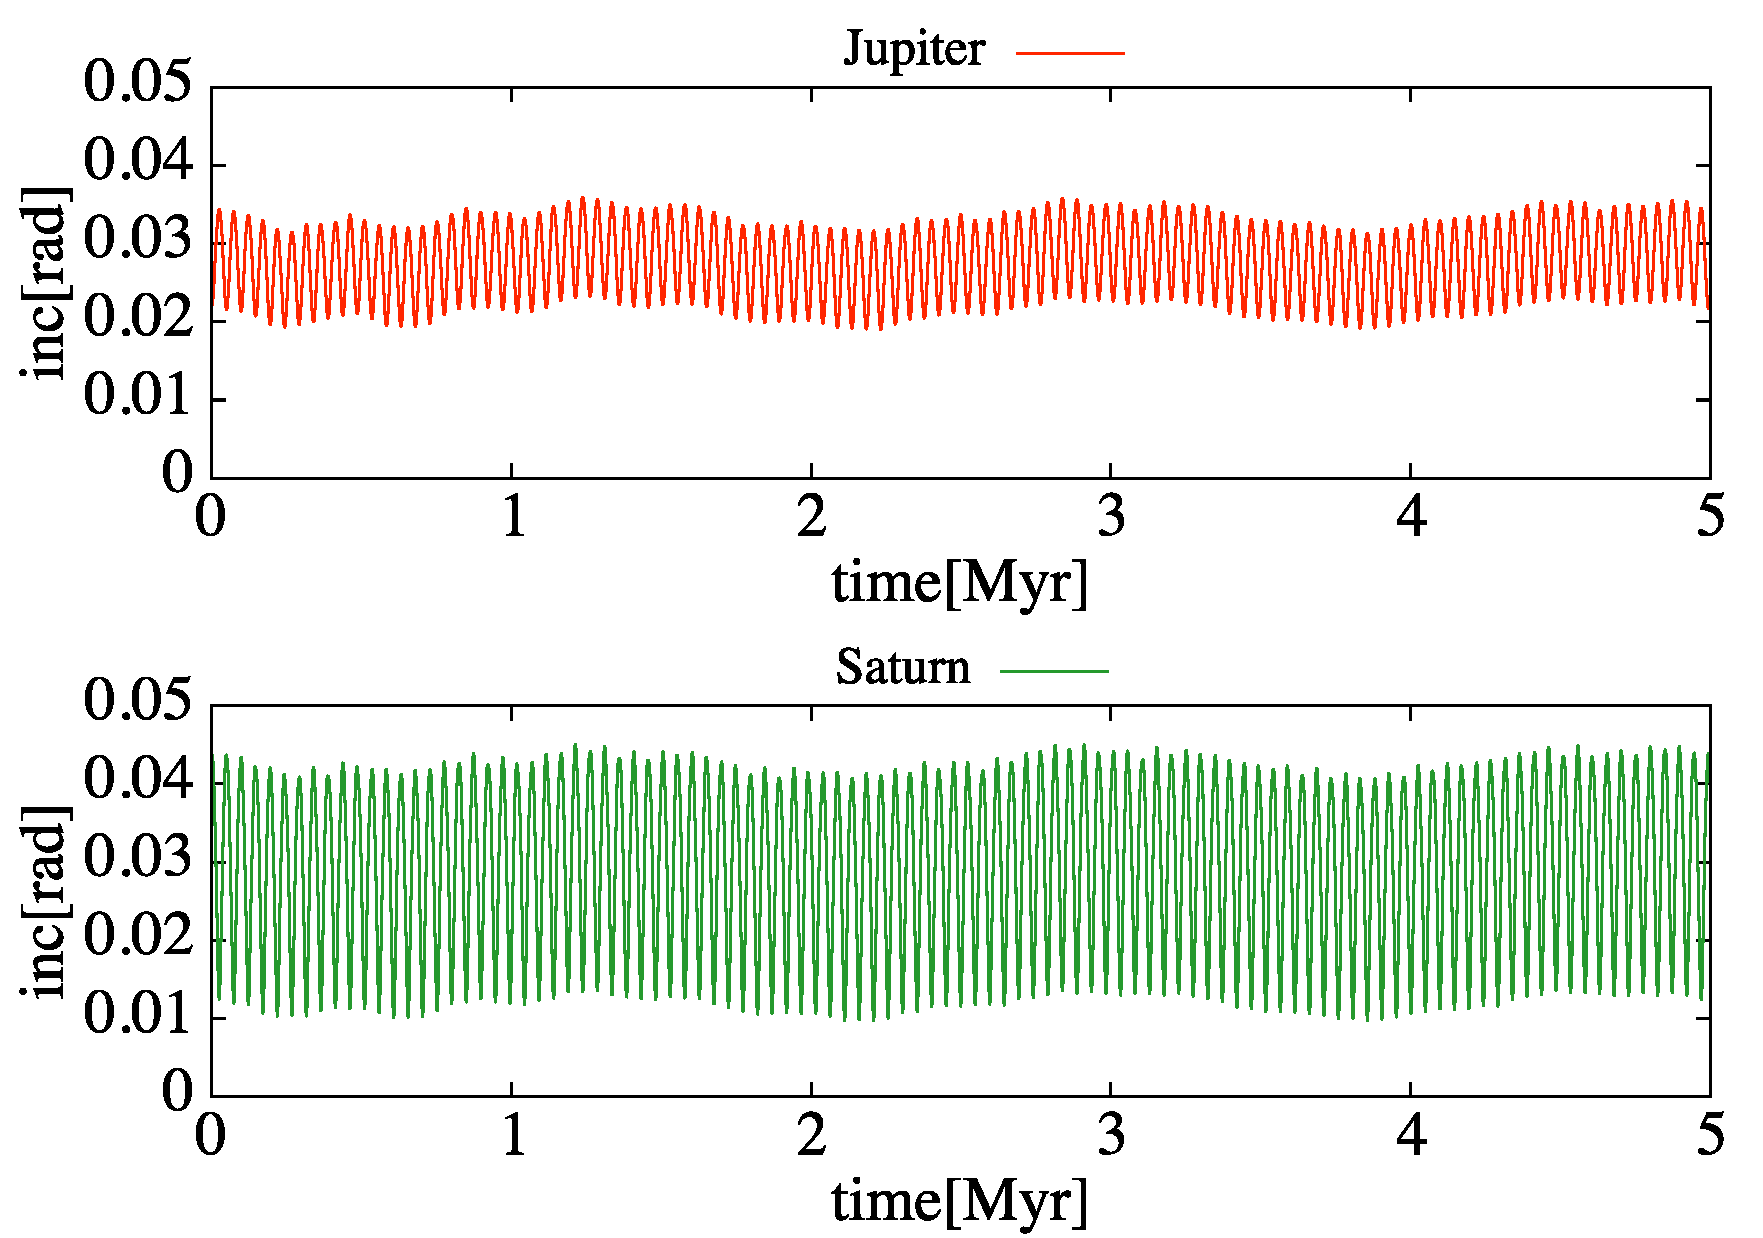
\includegraphics[width=8cm]{./image/NoMove_inc_5Myr_JUPSAT.pdf}
\end{minipage} &
%調整
\begin{minipage}[t]{0.1\hsize}
\end{minipage} &
%右
\begin{minipage}[t]{0.45\hsize}
\centering
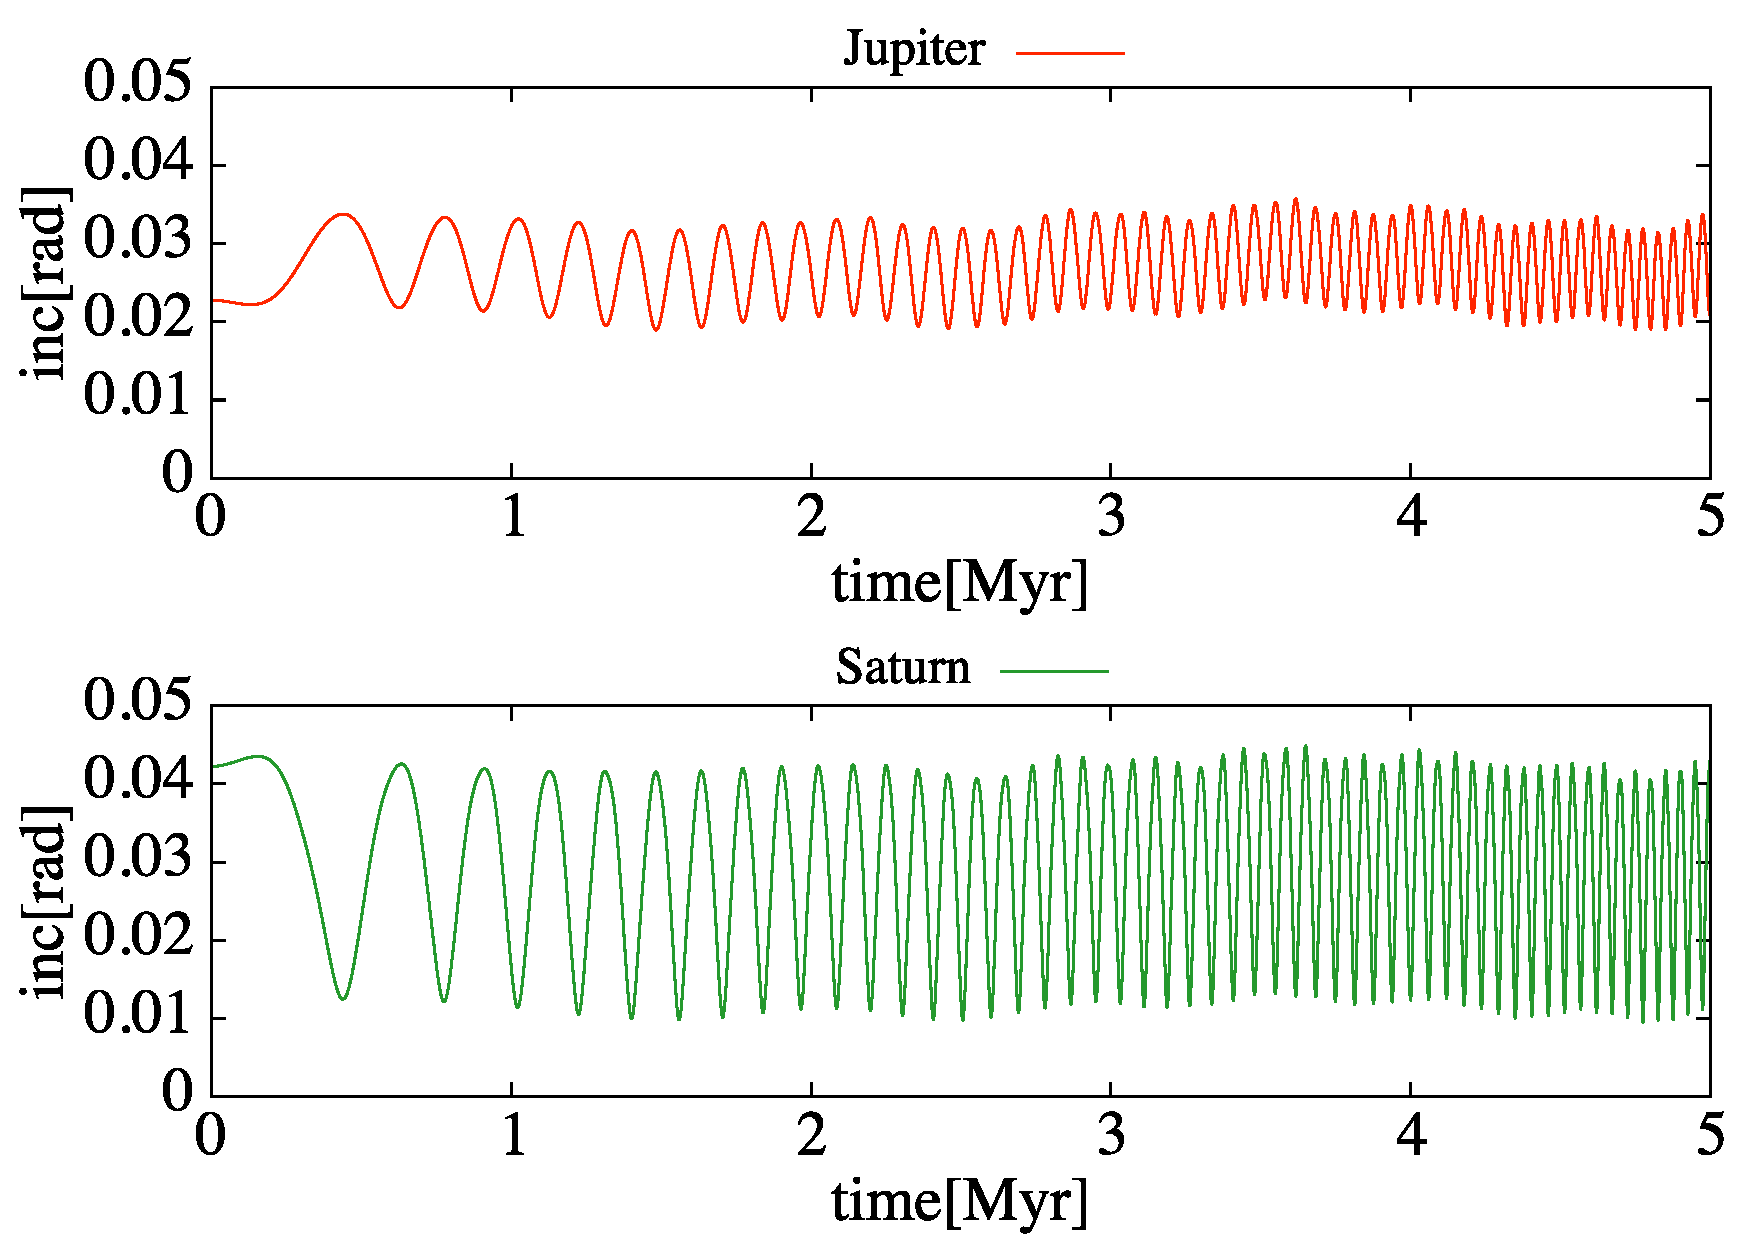
\includegraphics[width=8cm]{./image/Move500kyr_inc_5Myr_JUPSAT.pdf}
\end{minipage}\\
%左
\begin{minipage}[t]{0.45\hsize}
\centering
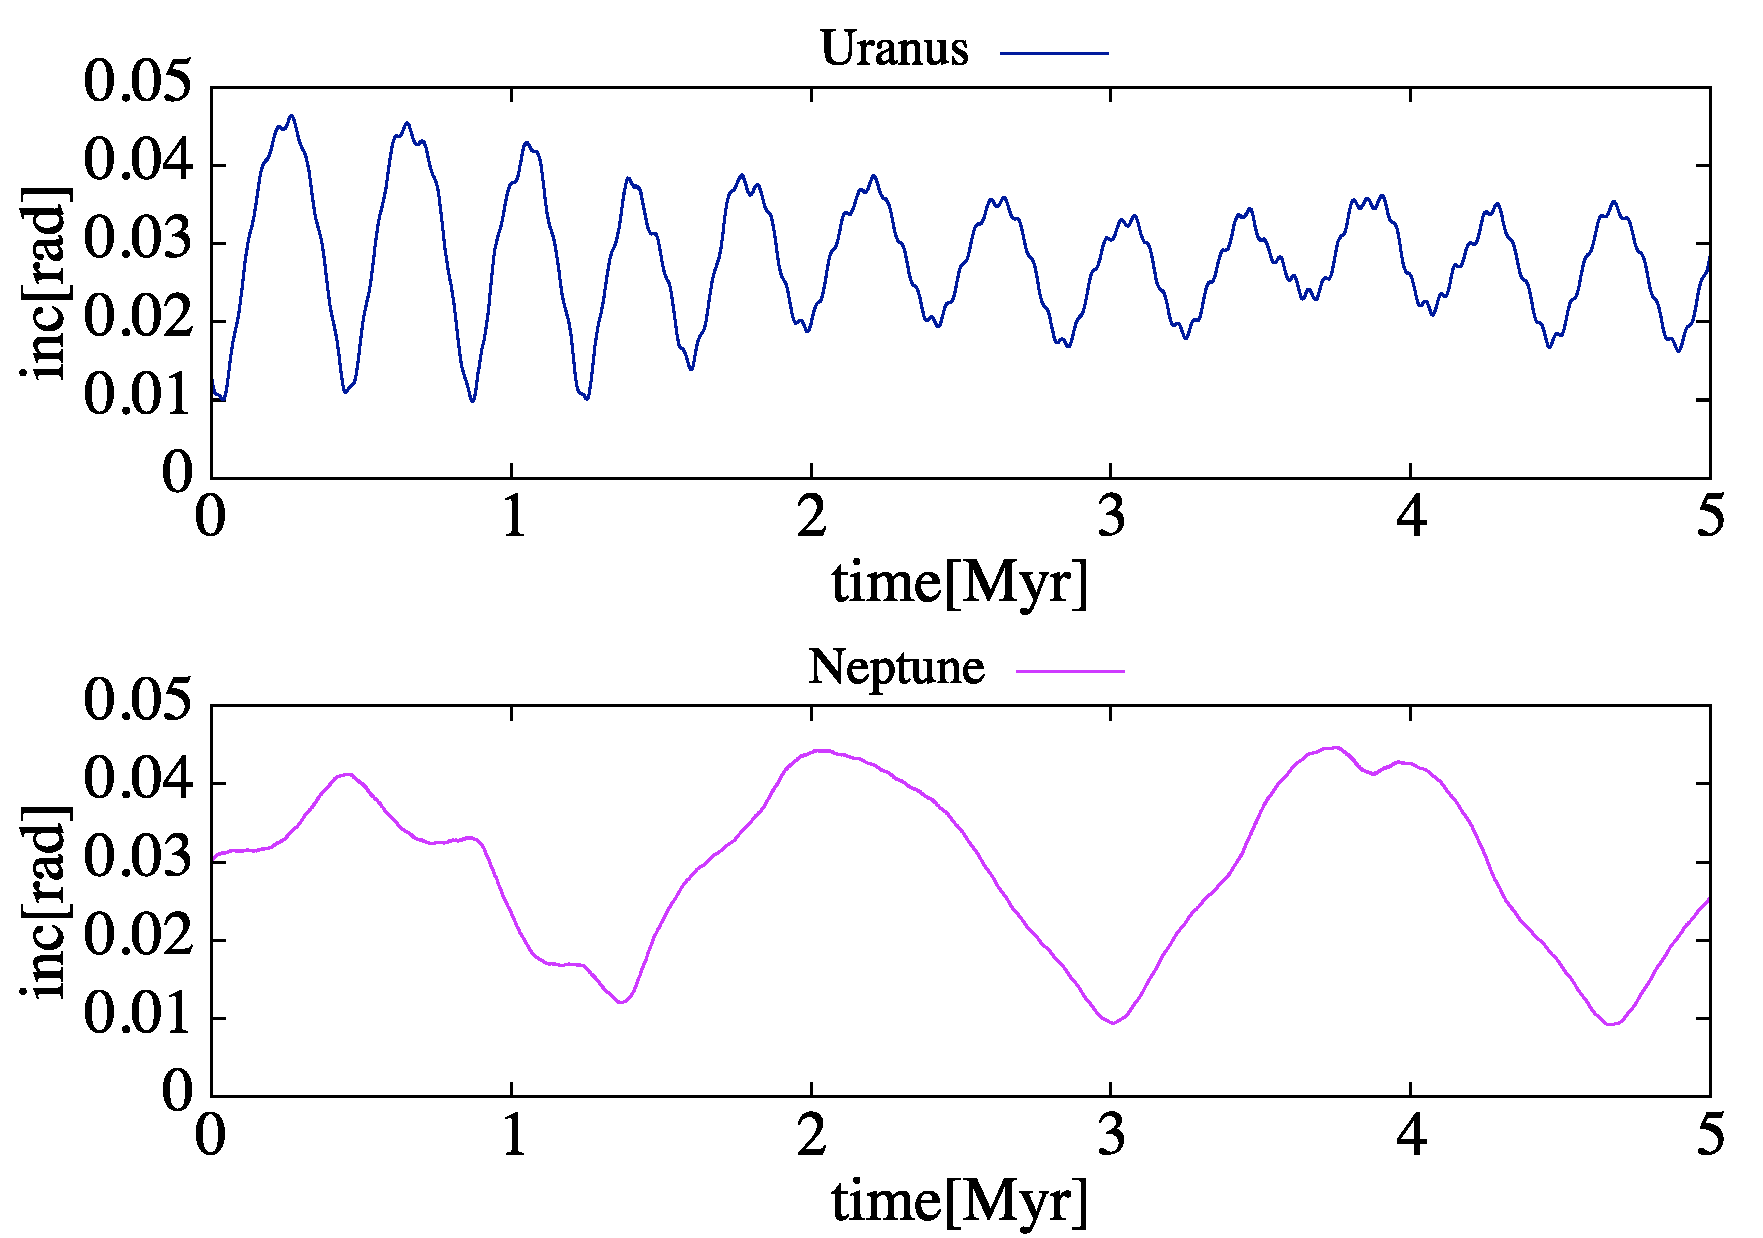
\includegraphics[width=8cm]{./image/NoMove_inc_5Myr_URANEP.pdf}
\end{minipage} &
%調整
\begin{minipage}[t]{0.1\hsize}
\end{minipage} &
%右
\begin{minipage}[t]{0.45\hsize}
\centering
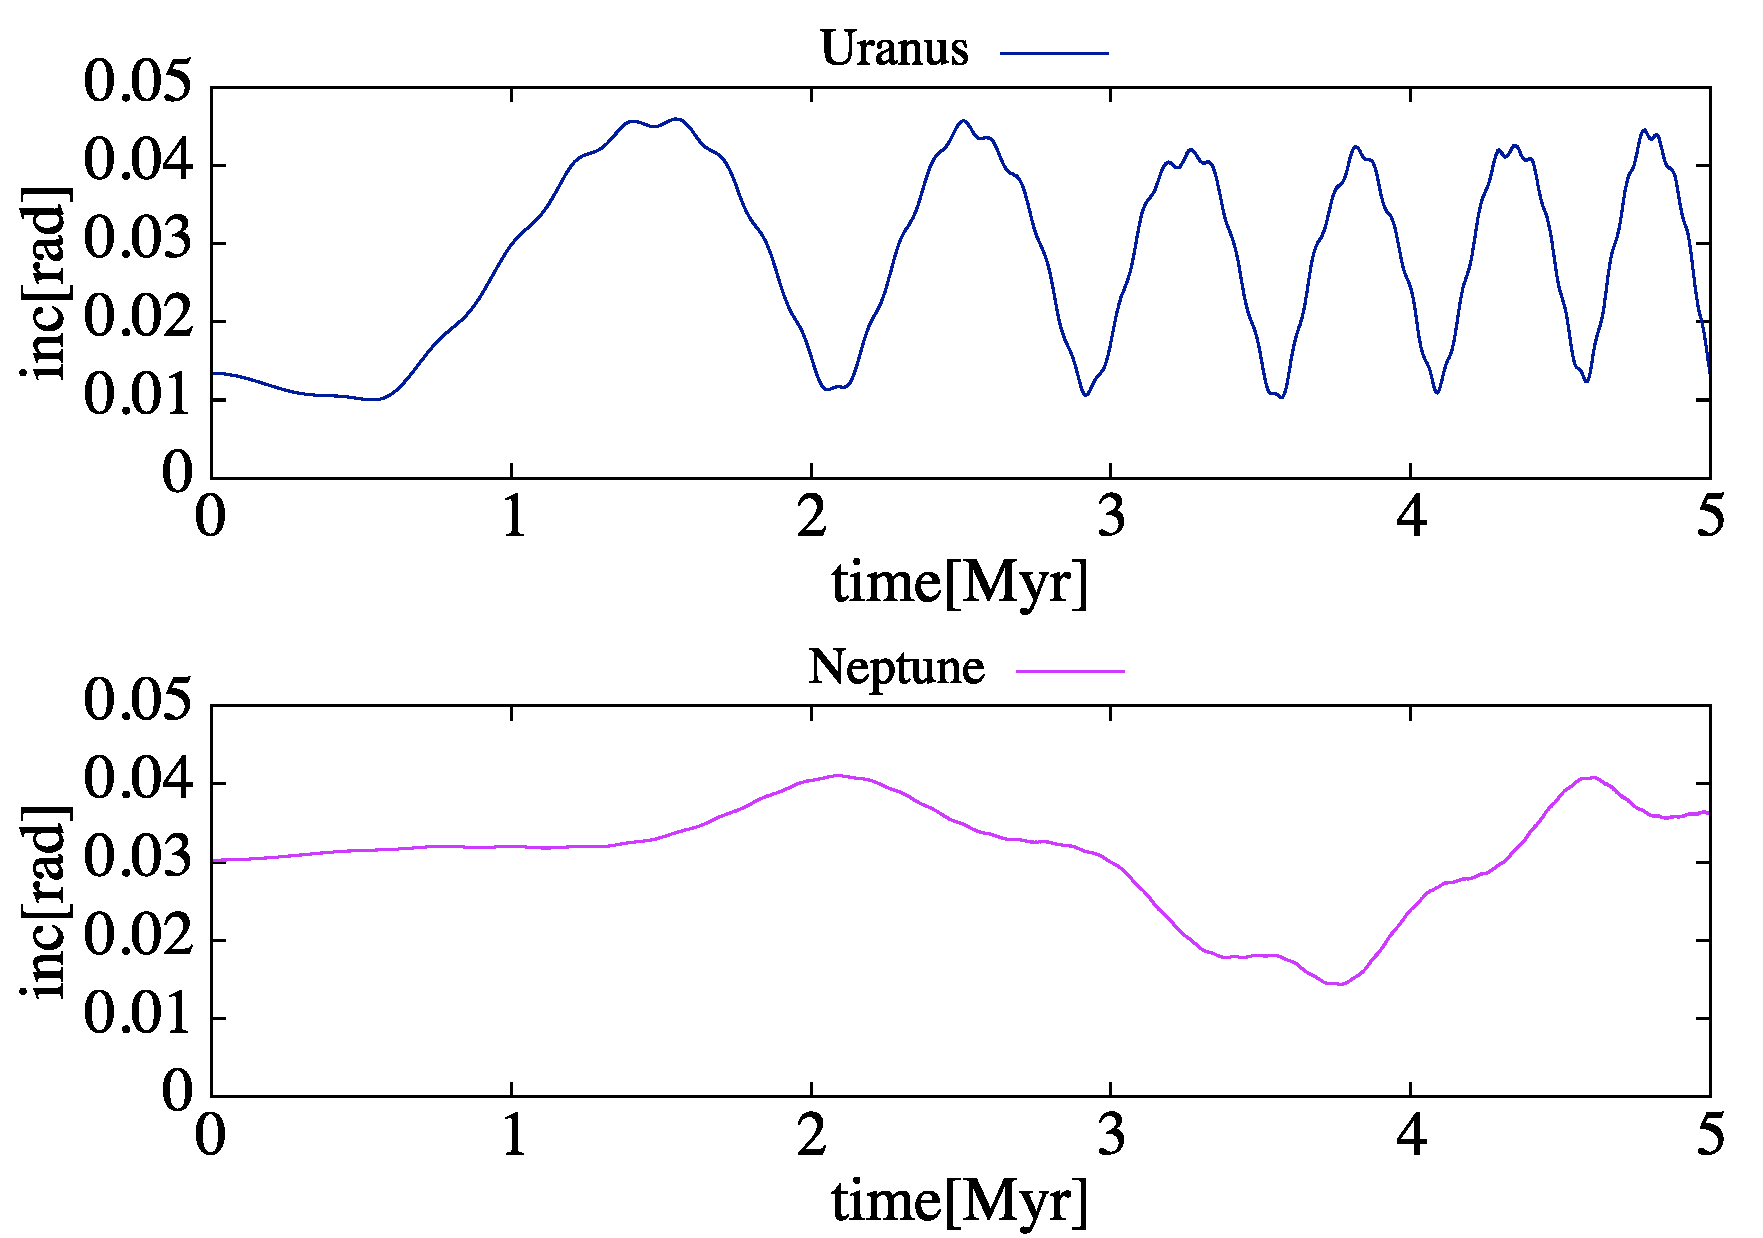
\includegraphics[width=8cm]{./image/Move500kyr_inc_5Myr_URANEP.pdf}
\end{minipage}
%
\end{tabular}
\caption{軌道傾斜角の変化.左が惑星移動なしの場合,右が惑星移動ありの場合,上から順に木星,土星,天王星,海王星である.\label{fig:inc}}
\end{figure}


\begin{figure}[H]
\begin{tabular}{ccc}
%左
\begin{minipage}[t]{0.45\hsize}
\centering
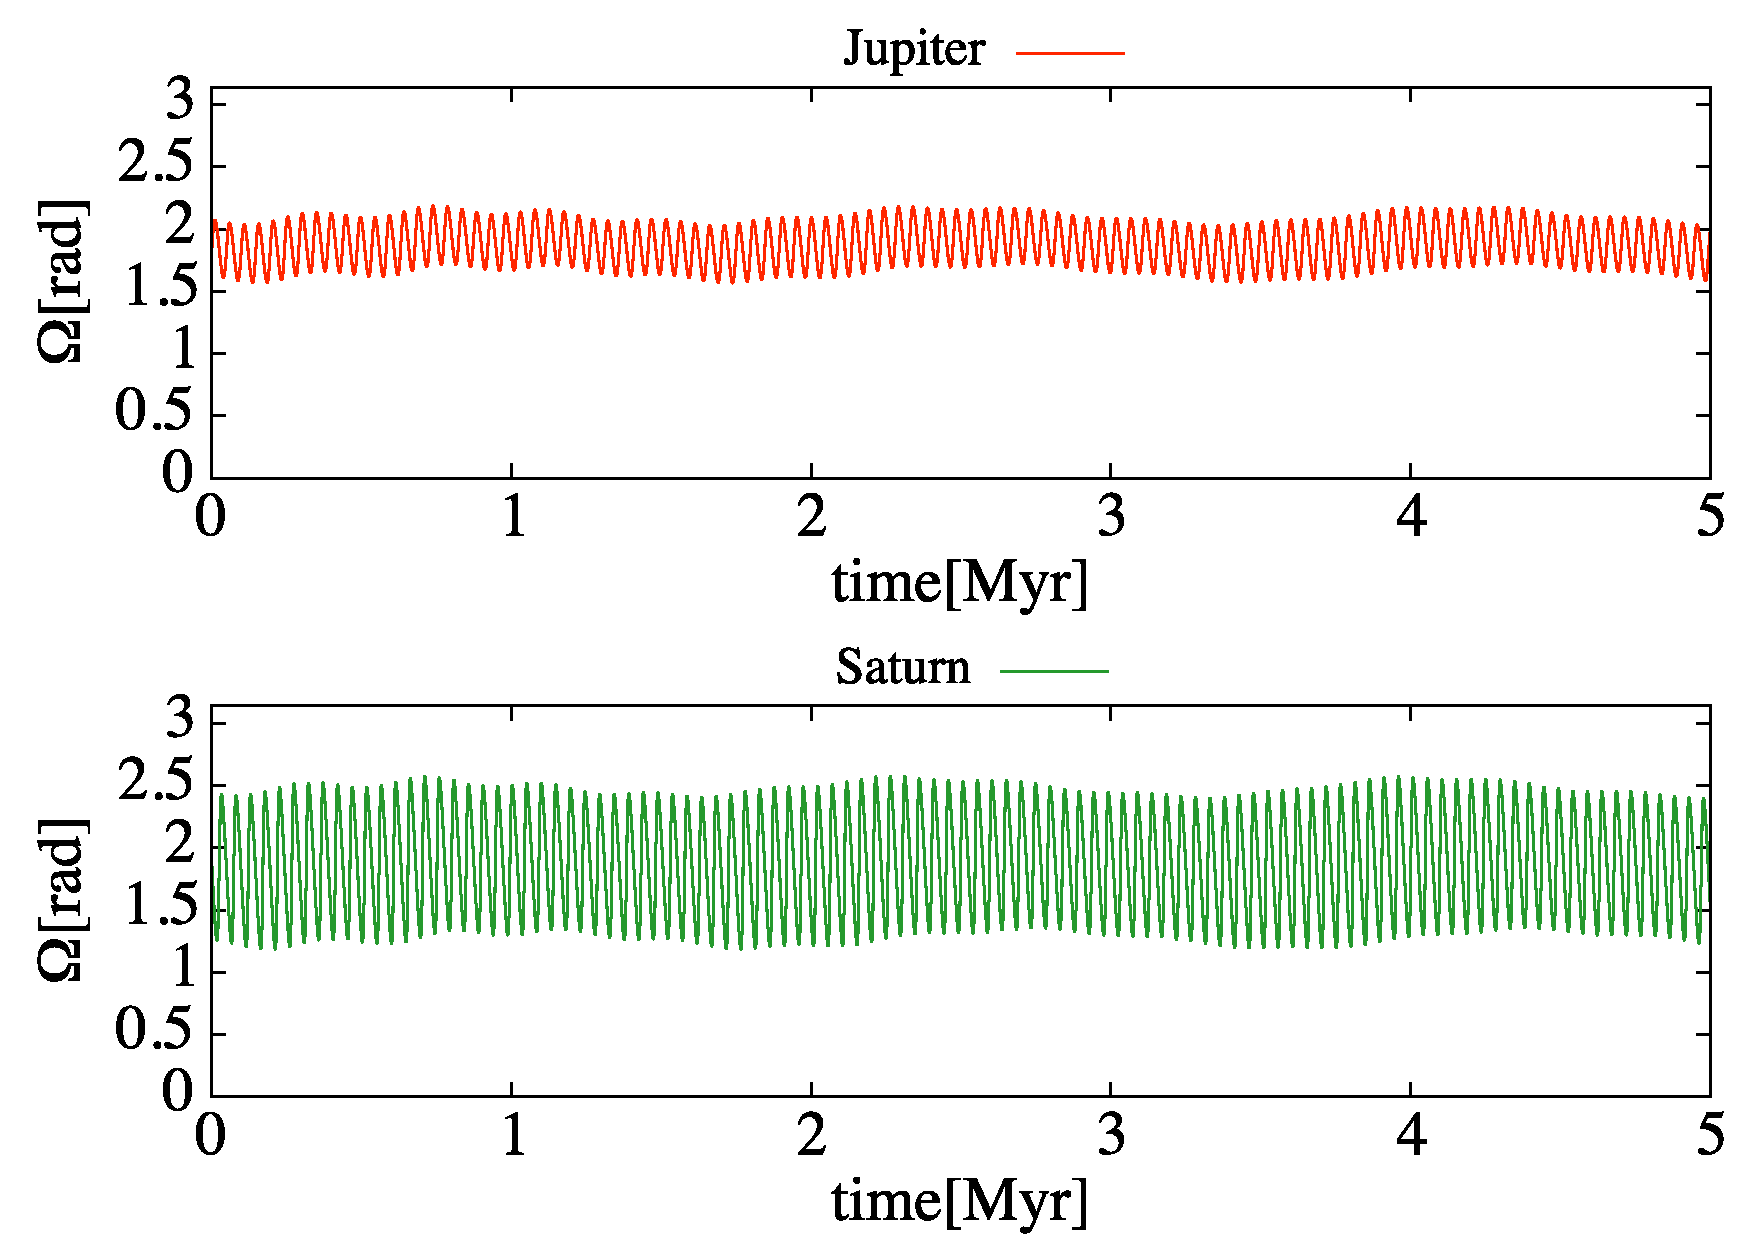
\includegraphics[width=8cm]{./image/NoMove_capitalOMEGA_5Myr_JUPSAT.pdf}
\end{minipage} &
%調整
\begin{minipage}[t]{0.1\hsize}
\end{minipage} &
%右
\begin{minipage}[t]{0.45\hsize}
\centering
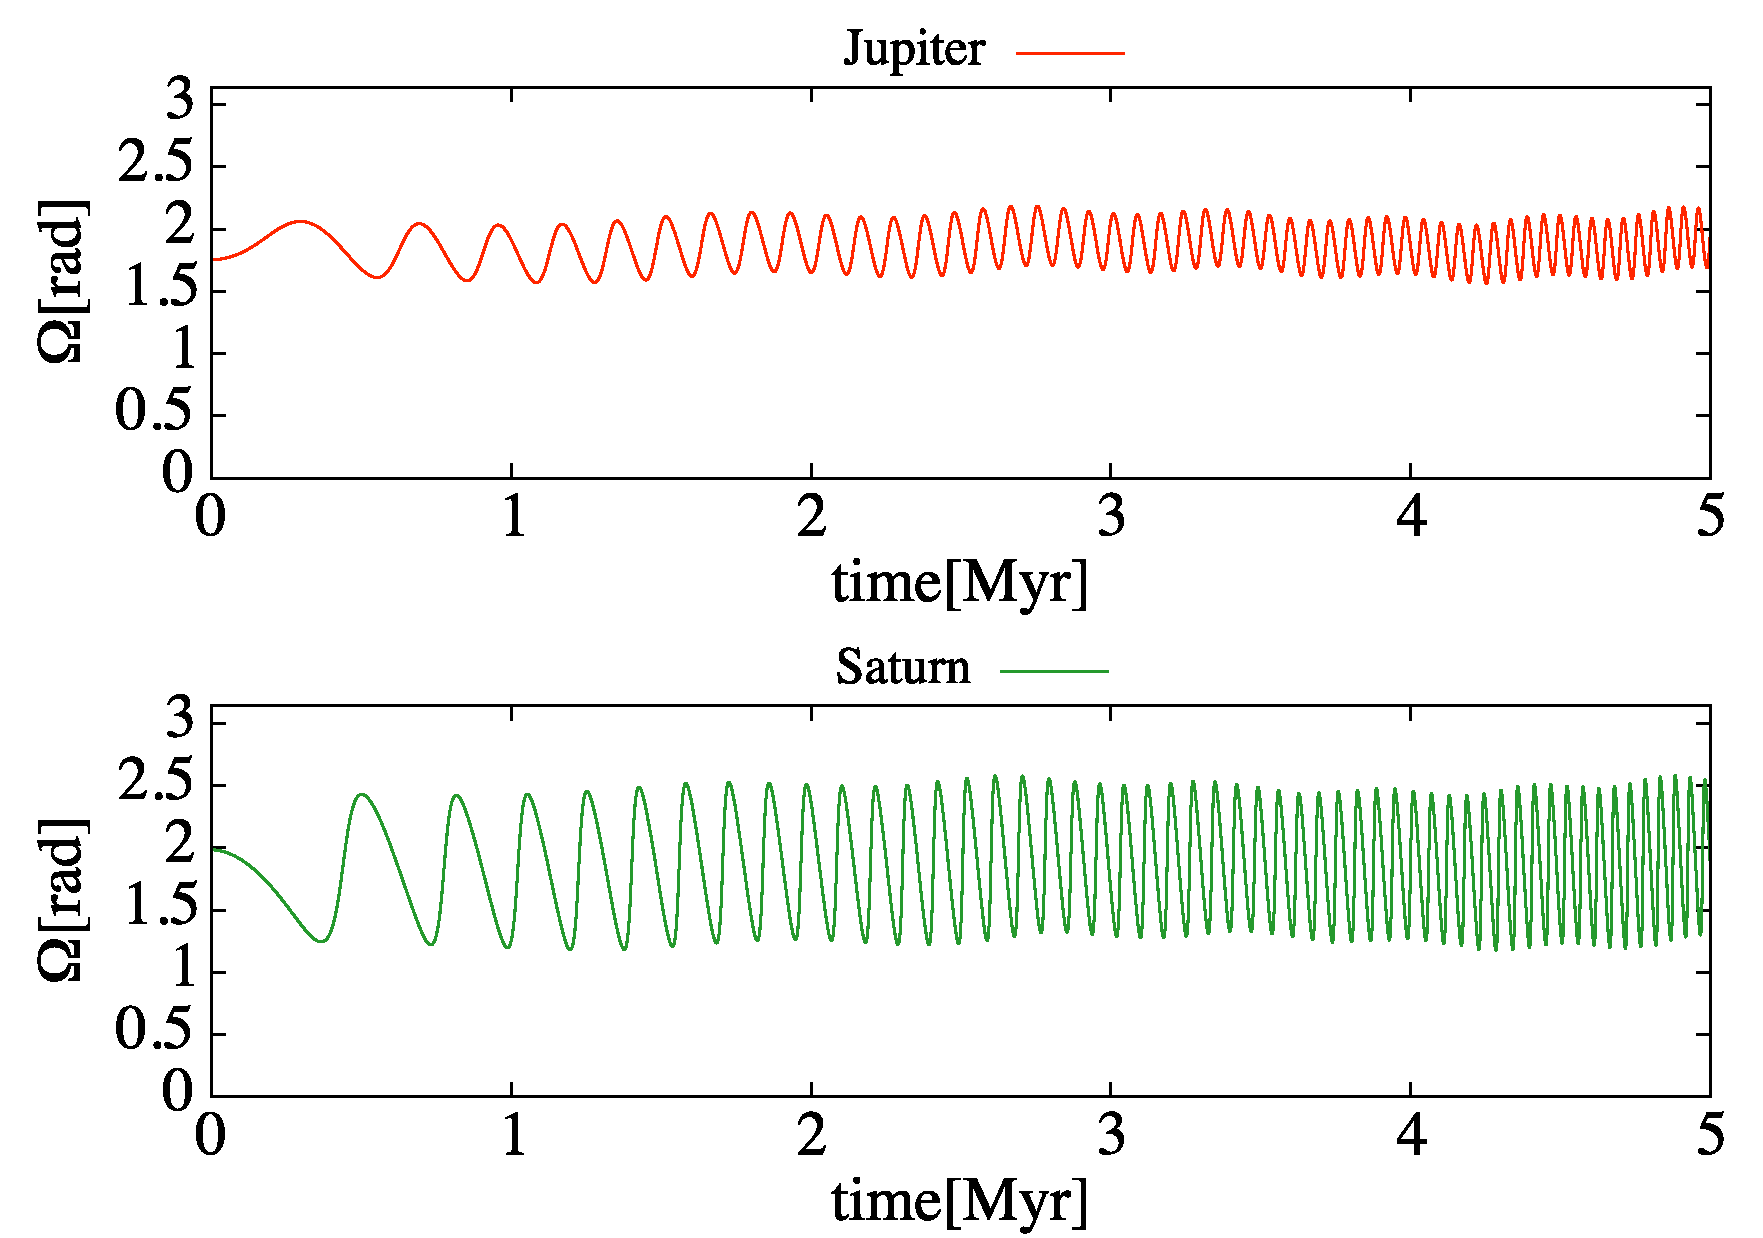
\includegraphics[width=8cm]{./image/Move500kyr_capitalOMEGA_5Myr_JUPSAT.pdf}
\end{minipage}\\
%左
\begin{minipage}[t]{0.45\hsize}
\centering
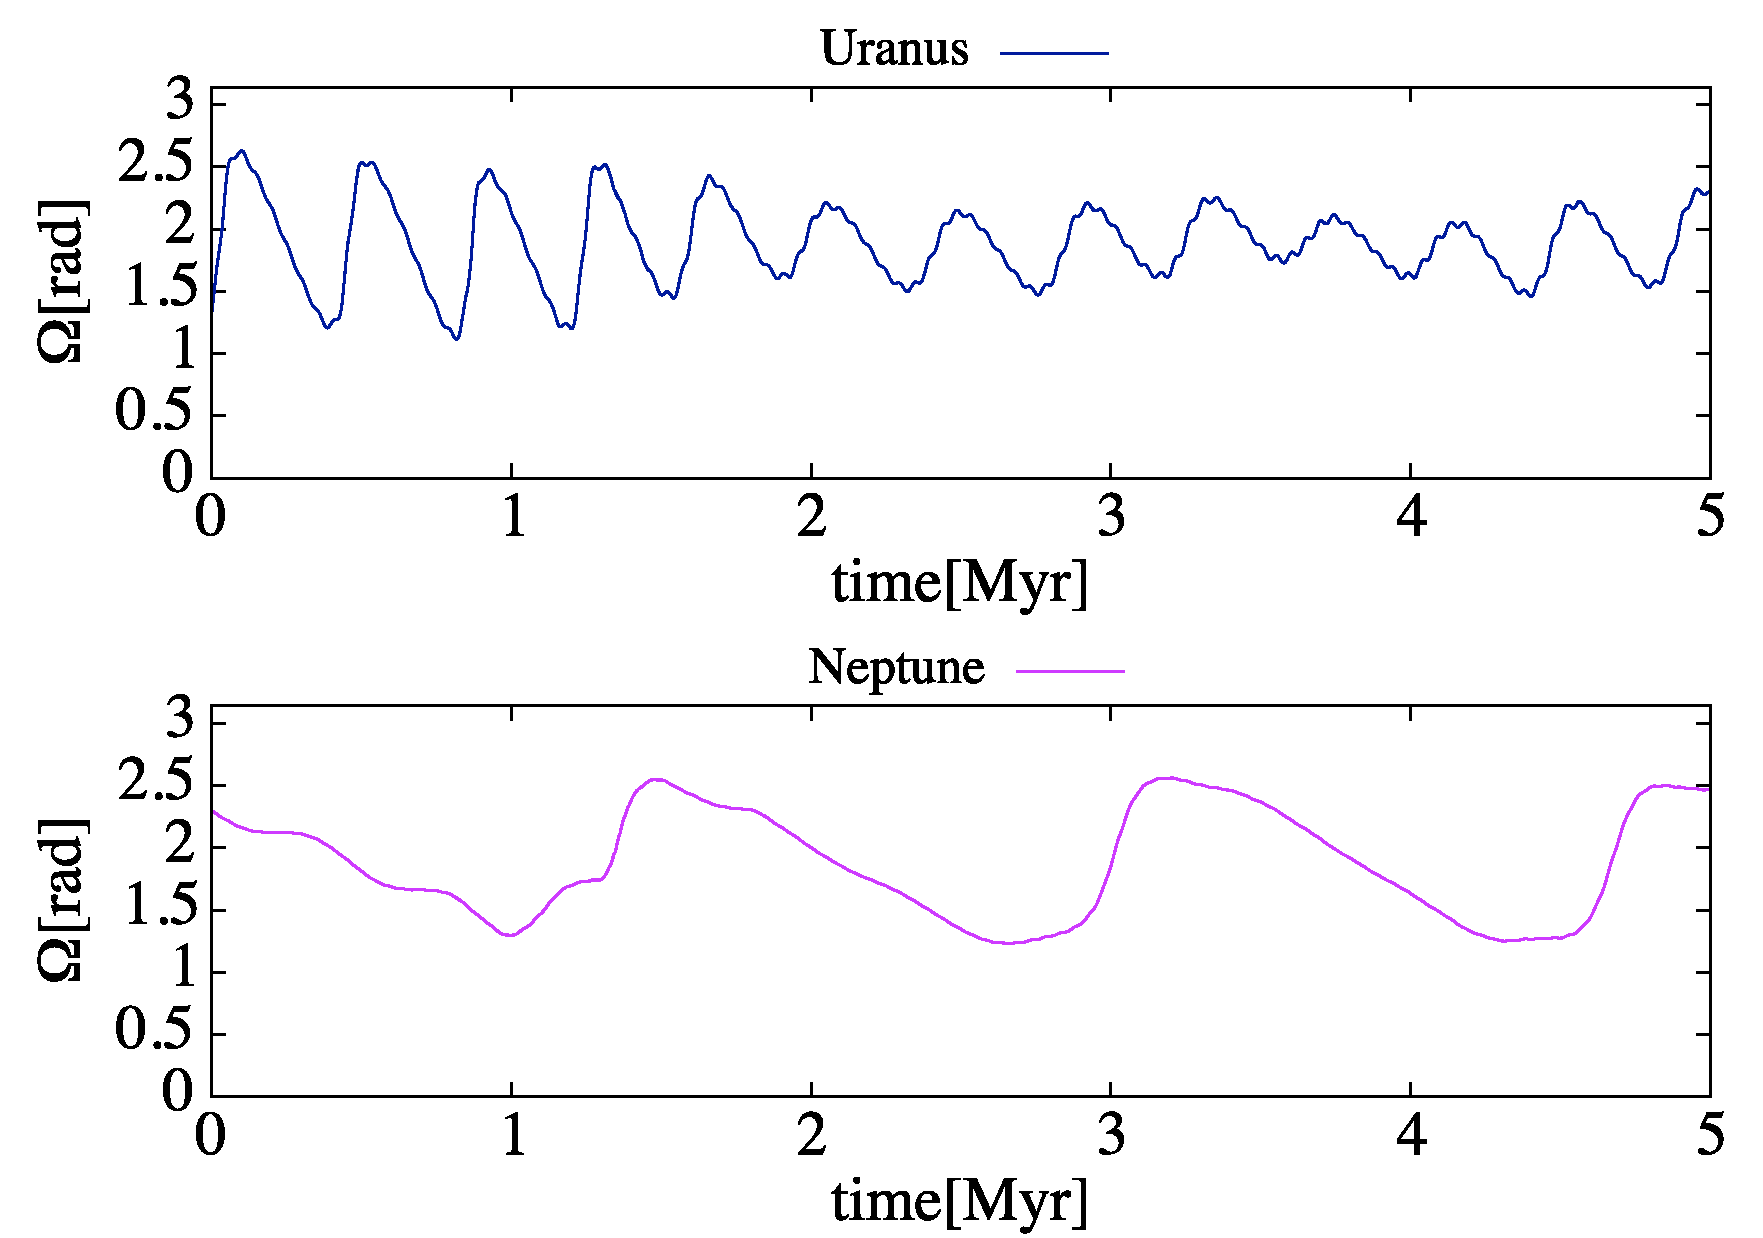
\includegraphics[width=8cm]{./image/NoMove_capitalOMEGA_5Myr_URANEP.pdf}
\end{minipage} &
%調整
\begin{minipage}[t]{0.1\hsize}
\end{minipage} &
%右
\begin{minipage}[t]{0.45\hsize}
\centering
\includegraphics[width=8cm]{./image/Move500kyr_capitalOMEGA_5Myr_URANEP.pdf}
\end{minipage}
%
\end{tabular}
\caption{昇交点経度の変化.左が惑星移動なしの場合,右が惑星移動ありの場合,上から順に木星,土星,天王星,海王星である.\label{fig:OMEGA}}
\end{figure}


\begin{figure}[H]
\begin{tabular}{ccc}
%左
\begin{minipage}[t]{0.45\hsize}
\centering
\includegraphics[width=8cm]{./image/NoMove_smallomega_5Myr_JUPSAT.pdf}
\end{minipage} &
%調整
\begin{minipage}[t]{0.1\hsize}
\end{minipage} &
%右
\begin{minipage}[t]{0.45\hsize}
\centering
\includegraphics[width=8cm]{./image/Move500kyr_smallomega_5Myr_JUPSAT.pdf}
\end{minipage}\\
%左
\begin{minipage}[t]{0.45\hsize}
\centering
\includegraphics[width=8cm]{./image/NoMove_smallomega_5Myr_URANEP.pdf}
\end{minipage} &
%調整
\begin{minipage}[t]{0.1\hsize}
\end{minipage} &
%右
\begin{minipage}[t]{0.45\hsize}
\centering
\includegraphics[width=8cm]{./image/Move500kyr_smallomega_5Myr_URANEP.pdf}
\end{minipage}
%
\end{tabular}
\caption{近日点引数の変化.左が惑星移動なしの場合,右が惑星移動ありの場合,上から順に木星,土星,天王星,海王星である.\label{fig:omega}}
\end{figure}


\begin{figure}[H]
\begin{tabular}{ccc}
%左
\begin{minipage}[t]{0.45\hsize}
\centering
\includegraphics[width=8cm]{./image/NoMove_curlypi_5Myr_JUPSAT.pdf}
\end{minipage} &
%調整
\begin{minipage}[t]{0.1\hsize}
\end{minipage} &
%右
\begin{minipage}[t]{0.45\hsize}
\centering
\includegraphics[width=8cm]{./image/Move500kyr_curlypi_5Myr_JUPSAT.pdf}
\end{minipage}\\
%左
\begin{minipage}[t]{0.45\hsize}
\centering
\includegraphics[width=8cm]{./image/NoMove_curlypi_5Myr_URANEP.pdf}
\end{minipage} &
%調整
\begin{minipage}[t]{0.1\hsize}
\end{minipage} &
%右
\begin{minipage}[t]{0.45\hsize}
\centering
\includegraphics[width=8cm]{./image/Move500kyr_curlypi_5Myr_URANEP.pdf}
\end{minipage}
%
\end{tabular}
\caption{近日点経度の変化.左が惑星移動なしの場合,右が惑星移動ありの場合,上から順に木星,土星,天王星,海王星である.\label{fig:varpi}}
\end{figure}



\subsubsection{永年共鳴の位置}
\ref{sec:2planet}節で扱った,2つの惑星の永年摂動を4つの惑星に拡張すると,
\begin{equation}
\begin{split}
{\cal R}_j = n_j^2 a_j^2 & \left[ \frac{1}{2} A_{jj} e_j^2 + \frac{1}{2} B_{jj} I_j^2 \right. \\
& + \left. \sum_{k = 1, k \not= j}^4 A_{jk} e_j e_k \cos (\varpi_j - \varpi_k) + \sum_{k = 1, k \not= j}^4 B_{jk} I_j I_k \cos (\Omega_j - \Omega_k) \right]. \\
\end{split} \label{}
\end{equation}
ここで,$j = 1, 2, 3, 4 (j \not= k)$ であり,
\begin{eqnarray}
A_{jj} & = & + n_j \frac{1}{4} \sum_{k = 1, k \not= j}^4 \frac{m_k}{m_c + m_j} \alpha_{jk} \bar{\alpha}_{jk} b_{3/2}^{(1)} (\alpha_{jk}), \\
A_{jk} & = & - n_j \frac{1}{4} \frac{m_k}{m_c + m_j} \alpha_{jk} \bar{\alpha}_{jk} b_{3/2}^{(2)} (\alpha_{jk}), \\
B_{jj} & = & - n_j \frac{1}{4} \sum_{k = 1, k \not= j}^4 \frac{m_k}{m_c + m_j} \alpha_{jk} \bar{\alpha}_{jk} b_{3/2}^{(1)} (\alpha_{jk}), \\
B_{jk} & = & + n_j \frac{1}{4} \frac{m_k}{m_c + m_j} \alpha_{jk} \bar{\alpha}_{jk} b_{3/2}^{(1)} (\alpha_{jk}). 
\end{eqnarray}
\begin{equation}
\alpha_{jk} = \left\{
\begin{array}{llll}
a_k / a_j & {\rm if} & a_j > a_k & \quad ({\rm internal \ perturber}), \\
a_j / a_k & {\rm if} & a_j < a_k & \quad ({\rm external \ perturber}).
\end{array}
\right.
\end{equation}
\begin{equation}
\bar{\alpha}_{jk} = \left\{
\begin{array}{llll}
1 & {\rm if} & a_j > a_k & \quad ({\rm internal \ perturber}), \\
a_j / a_k & {\rm if} & a_j < a_k & \quad ({\rm external \ perturber}).
\end{array}
\right.
\end{equation}
また,
\begin{equation}
h_j = e_j \sin \varpi_j, \quad k_j = e_j \cos \varpi_j,
\end{equation}
\begin{equation}
p_j = I_j \sin \Omega_j, \quad q_j = I_j \cos \Omega_j.
\end{equation}
と定義される変数を用いて,
\begin{equation}
\begin{split}
{\cal R}_j = n_j a_j^2 & \left[ \frac{1}{2} A_{jj} (h_j^2 + k_j^2) + \frac{1}{2} B_{jj} (p_j^2 + q_j^2) \right. \\
& + \left. \sum_{k = 1, k \not= j}^4 A_{jk} (h_j h_k + k_j k_k) + \sum_{k = 1, k \not= j}^4 B_{jk} (p_j p_k + q_j q_k) \right]. \\
\end{split} \label{}
\end{equation}
ラグランジュの惑星方程式の最低次までの近似形を用いると,この問題は4つの固有値問題にまとめられ,その解は,
\begin{equation}
h_j = \sum_{i = 1}^4 e_{ji} \sin (g_i t + \beta_i), \quad k_j = \sum_{i=1}^4 e_{ji} \cos (g_i t + \beta_i), \label{}
\end{equation}
\begin{equation}
p_j = \sum_{i = 1}^4 I_{ji} \sin (f_i t + \gamma_i), \quad q_j = \sum_{i=1}^4 I_{ji} \cos (f_i t + \gamma_i). \label{}
\end{equation}
ここで,振動数 $g_i (i = 1, 2, 3, 4)$ は行列 ${\rm A}$ の固有値,$e_{ji}$ は固有ベクトルの4つの要素に対応しており,また振動数 $f_i (i = 1, 2, 3, 4)$ は行列 ${\rm B}$ の固有値,$I_{ji}$ は固有ベクトルの4つの要素に対応している.位相 $\beta_i, \gamma_i$ は,固有ベクトルの振幅と同様に,初期条件によって決まる.任意の時間における質量 $m_j$ の惑星の離心率と軌道傾斜角の2乗の値は,
\begin{eqnarray}
e_j^2 & = & \left[ \sum_{i = 1}^4 e_{ji} \sin (g_i t + \beta_i) \right]^2 + \left[ \sum_{i = 1}^4 e_{ji} \cos (g_i t + \beta_i) \right]^2, \\
I_j^2 & = & \left[ \sum_{i = 1}^4 I_{ji} \sin (f_i t + \gamma_i) \right]^2 + \left[ \sum_{i = 1}^4 e_{ji} \cos (f_i t + \gamma_i) \right]^2.
\end{eqnarray}
同様に,$h_j, k_j, p_j, q_j$ の値から質量 $m_j$ の惑星の近日点経度や昇交点経度も求められる.

続いて,\ref{sec:free_forced}節で扱った自由要素と強制要素を,4つの惑星がある場合に拡張すると,
\begin{equation}
\begin{split}
{\cal R} = n a^2 & \left[ \frac{1}{2} A e^2 + \frac{1}{2} B I^2 \right. \\
& \left. + \sum_{j = 1}^4  A_j e e_j \cos (\varpi - \varpi_j) + \sum_{j = 1}^4 B_j I I_j \cos (\Omega - \Omega_j) \right]. \\
\end{split} \label{}
\end{equation} 
ここで,
\begin{eqnarray}
A & = & + n \frac{1}{4} \sum_{j = 1}^4 \frac{m_j}{m_c} \alpha_j \bar{\alpha}_j b_{3/2}^{(1)} (\alpha_j), \label{eq:A_test_4planet} \\
A_j & = & - n \frac{1}{4} \frac{m_j}{m_c} \alpha_j \bar{\alpha}_j b_{3/2}^{(2)} (\alpha_j), \label{eq:A_j_test_4planet} \\
B & = & - n \frac{1}{4} \sum_{j = 1}^4 \frac{m_j}{m_c} \alpha_j \bar{\alpha}_j b_{3/2}^{(1)} (\alpha_j), \label{eq:B_test_4planet} \\
B_j & = & + n \frac{1}{4} \frac{m_j}{m_c} \alpha_j \bar{\alpha}_j b_{3/2}^{(1)} (\alpha_j). \label{eq:B_j_test_4planet}
\end{eqnarray}
\begin{equation}
\alpha_j = \left\{
\begin{array}{lll}
a_j / a & {\rm if} & a_j < a, \\
a / a_j & {\rm if} & a_j > a,
\end{array}
\right.
\end{equation}
\begin{equation}
\bar{\alpha}_j = \left\{
\begin{array}{lll}
1 & {\rm if} & a_j < a, \\
a / a_j & {\rm if} & a_j > a.
\end{array}
\right.
\end{equation}
また,
\begin{eqnarray}
h = e \sin \varpi, & \quad & k = e \cos \varpi, \\
p = I \sin \Omega, & \quad & q = I \cos \Omega.
\end{eqnarray}
と定義される変数を用いて,
\begin{equation}
\begin{split}
{\cal R} = n a^2 & \left[ \frac{1}{2} A (h^2 + k^2) + \frac{1}{2} B (p^2 + q^2) \right. \\
& \left. + \sum_{j = 1}^4 A_j (h h_j + k k_j) + \sum_{j = 1}^4 B_j (p p_j + q q_j) \right]. \\
\end{split} \label{}
\end{equation}
ラグランジュの惑星方程式の最低次までの近似形を用いると,線形微分方程式にまとめられ,その解は,
\begin{eqnarray}
h = e_{\rm free} \sin (A t + \beta) + h_0 (t), & \quad & k = e_{\rm free} \cos (A t + \beta) + k_0 (t), \label{eq:hk_solution} \\
p = I_{\rm free} \sin (B t + \gamma) + p_0 (t), & \quad & q = I_{\rm free} \cos (B t + \gamma) + q_0 (t). \label{eq:pq_solution}
\end{eqnarray}
ここで,$e_{\rm free}, I_{\rm free}, \beta, \gamma$ は境界条件から決まる定数であり,
\begin{eqnarray}
h_0 (t) & = & - \sum_{i = 1}^4 \frac{\nu_i}{A - g_i} \sin (g_i t + \beta_i), \label{eq:h_0_4planet} \\
k_0 (t) & = & - \sum_{i = 1}^4 \frac{\nu_i}{A - g_i} \cos (g_i t + \beta_i), \label{eq:k_0_4planet} \\
p_0 (t) & = & - \sum_{i = 1}^4 \frac{\mu_i}{B - f_i} \sin (f_i t + \gamma_i), \label{eq:p_0_4planet} \\
q_0 (t) & = & - \sum_{i = 1}^4 \frac{\mu_i}{B - f_i} \cos (f_i t + \gamma_i). \label{eq:q_0_4planet}
\end{eqnarray}
\begin{equation}
\nu_i = \sum_{j = 1}^4 A_j e_{ji} \quad {\rm and} \quad \mu_i = \sum_{j=1}^4 B_j I_{ji}. \label{eq:nu_mu_4planet}
\end{equation}
強制離心率と強制軌道傾斜角は,
\begin{equation}
e_{\rm forced} = \sqrt{h_0^2 + k_0^2}, \quad I_{\rm forced} = \sqrt{p_0^2 + q_0^2} \label{eq:forced}
\end{equation}
と定義される.

式(\ref{eq:h_0_4planet})から式(\ref{eq:q_0_4planet})より,$A$ の値が $g_i$,$B$ の値が $f_i$ と一致する場合に発散が生じることは明らかである.図\ref{fig:PrecessionRate}は,それぞれの惑星の固有振動数 $g_i, f_i$(定数)と,テスト粒子の $A = g_t, B = f_t$ を軌道長半径の関数としてプロットしたものである.添字については,$t : テスト粒子$,$5 : 木星$,$6 : 土星$,$7 : 天王星$,$8 : 海王星$ としている(太陽系第 $i$ 惑星に対応させている).式(\ref{eq:A_test_4planet}),式(\ref{eq:B_test_4planet})の定義より,中心星を質点と扱う場合 $A = - B$ であるから,$g_t, - f_t$ は重なっている.
\begin{figure}[H]
\centering
\includegraphics[width=8cm]{./image/PrecessionRate_logAB.pdf}
\caption{惑星の固有振動数 $g_i, f_i$(定数)と,テスト粒子の $A = g_t, B = f_t$ を軌道長半径の関数としてプロットした.縦軸の歳差率の単位は「秒角/年」である.$g_t, - f_t$ が発散している位置はそれぞれの惑星の軌道長半径である.\label{fig:PrecessionRate}}
\end{figure}
この図から,$g_t = g_i$ となる交点の軌道長半径は離心率の永年共鳴の位置となることが分かり,その位置を $\nu_i$ と表記する( 式(\ref{eq:nu_mu_4planet})の $\nu_i$ と全く異なるので注意).同様に,$f_t = f_i$ となる交点の軌道長半径は軌道傾斜角の永年共鳴の位置となることが分かり,その位置を $\nu_{1i}$ と表記する.惑星の固有振動数 $g_i, f_i$ とテスト粒子の $A, B$ は軌道長半径に依存するため,惑星の移動に伴いどちらも時間変化し,ゆえに交点の位置 $\nu_i, \nu_{1i}$ も時間変化する.図\ref{fig:SecularResonanceAxis_ecc},図\ref{fig:SecularResonanceAxis_ecc_upto5AU}は離心率の永年共鳴の位置を数値計算で求めた結果である.
\begin{figure}[H]
\centering
\includegraphics[width=8cm]{./image/SecularResonanceAxis_ecc.pdf}
\caption{離心率の永年共鳴の位置の時間変化.添字は $5 : 木星$,$6 : 土星$,$7 : 天王星$,$8 : 海王星$.軌道長半径の範囲は0AU - 50AUである.\label{fig:SecularResonanceAxis_ecc}}
\end{figure}

\begin{figure}[H]
\centering
\includegraphics[width=8cm]{./image/SecularResonanceAxis_ecc_upto5AU.pdf}
\caption{離心率の永年共鳴の位置の時間変化(小惑星帯付近を拡大).添字は $5 : 木星$,$6 : 土星$,$7 : 天王星$,$8 : 海王星$.軌道長半径の範囲は0AU - 5AUである.\label{fig:SecularResonanceAxis_ecc_upto5AU}}
\end{figure}

土星による離心率の永年共鳴の位置 $\nu_6$ が小惑星帯領域(2AU - 4AU)の一部を通過していることが分かる.

続いて,図\ref{fig:SecularResonanceAxis_inc},図\ref{fig:SecularResonanceAxis_inc_upto5AU}は軌道傾斜角の永年共鳴の位置を数値計算で求めた結果である.

\begin{figure}[H]
\centering
\includegraphics[width=8cm]{./image/SecularResonanceAxis_inc.pdf}
\caption{軌道傾斜角の永年共鳴の位置の時間変化.添字は $15 : 木星$,$16 : 土星$,$17 : 天王星$,$18 : 海王星$.軌道長半径の範囲は0AU - 50AUである.\label{fig:SecularResonanceAxis_inc}}
\end{figure}

\begin{figure}[H]
\centering
\includegraphics[width=8cm]{./image/SecularResonanceAxis_inc_upto5AU.pdf}
\caption{軌道傾斜角の永年共鳴の位置の時間変化(小惑星帯付近を拡大).添字は $15 : 木星$,$16 : 土星$,$17 : 天王星$,$18 : 海王星$.軌道長半径の範囲は0AU - 5AUである.\label{fig:SecularResonanceAxis_inc_upto5AU}}
\end{figure}

土星による軌道傾斜角の永年共鳴の位置 $\nu_{16}$ が小惑星帯領域(2AU - 4AU)の一部を通過していることが分かる.

\subsection{カイパーベルト}
今度は,カイパーベルトについて詳しく見るために,小天体の代わりにテスト粒子を1000個用意してカイパーベルト領域においた計算を20\ Myr行った.テスト粒子の初期条件は,軌道長半径 $a = 28.0 {\rm AU} - 52.0 {\rm AU}$,離心率 $e = 0 - 0.05$,軌道傾斜角 $I = 0\ {\rm rad} - 0.05\ {\rm rad}$,その他の角度に関する軌道要素 $0\ {\rm rad} - 2 \pi\ {\rm rad}$ の範囲の中でランダムに決めた.

以下の図は時間 $t = 0\ {\rm yr}, 1 \times 10^3\ {\rm yr}, 1 \times 10^4\ {\rm yr}, 1 \times 10^5\ {\rm yr}, 1 \times 10^6\ {\rm yr}, 1 \times 10^7\ {\rm yr}, 2 \times 10^7\ {\rm yr}$ におけるテスト粒子と海王星の離心率と軌道傾斜角をプロットしたものである.整数比が上に書かれている破線は海王星との平均運動共鳴の位置であり,$\nu_i, \nu_{1i}$ が上に書かれている破線は永年共鳴の位置を表している.また曲線は,近日点距離が海王星の軌道長半径と一致するときの,軌道長半径と離心率の関係を表している.海王星の円について,横軸方向の半径の大きさは海王星のヒル半径(AU)と等しい.初期に惑星の質量が0としたため,$t = 0\ {\rm yr}$ での海王星の円と永年共鳴の位置は定義できない.

\begin{figure}[H]
\begin{tabular}{ccc}
%左
\begin{minipage}[t]{0.45\hsize}
\centering
\includegraphics[width=8cm]{./image/kuiper_ecc_0yr.pdf}
\end{minipage} &
%調整
\begin{minipage}[t]{0.1\hsize}
\end{minipage} &
%右
\begin{minipage}[t]{0.45\hsize}
\centering
\includegraphics[width=8cm]{./image/kuiper_inc_0yr.pdf}
\end{minipage}\\
%
\end{tabular}
\caption{$t = 0\ {\rm yr}$ におけるテスト粒子と海王星の離心率(左)と軌道傾斜角(右).\label{fig:kuiper_ecc_inc_0yr}}
\end{figure}

\begin{figure}[H]
\begin{tabular}{ccc}
%左
\begin{minipage}[t]{0.45\hsize}
\centering
\includegraphics[width=8cm]{./image/kuiper_ecc_1kyr.pdf}
\end{minipage} &
%調整
\begin{minipage}[t]{0.1\hsize}
\end{minipage} &
%右
\begin{minipage}[t]{0.45\hsize}
\centering
\includegraphics[width=8cm]{./image/kuiper_inc_1kyr.pdf}
\end{minipage}\\
%
\end{tabular}
\caption{$t = 1 \times 10^3\ {\rm yr}$ におけるテスト粒子と海王星の離心率(左)と軌道傾斜角(右).\label{fig:kuiper_ecc_inc_1kyr}}
\end{figure}

\begin{figure}[H]
\begin{tabular}{ccc}
%左
\begin{minipage}[t]{0.45\hsize}
\centering
\includegraphics[width=8cm]{./image/kuiper_ecc_10kyr.pdf}
\end{minipage} &
%調整
\begin{minipage}[t]{0.1\hsize}
\end{minipage} &
%右
\begin{minipage}[t]{0.45\hsize}
\centering
\includegraphics[width=8cm]{./image/kuiper_inc_10kyr.pdf}
\end{minipage}\\
%
\end{tabular}
\caption{$t = 1 \times 10^4\ {\rm yr}$ におけるテスト粒子と海王星の離心率(左)と軌道傾斜角(右).\label{fig:kuiper_ecc_inc_10kyr}}
\end{figure}

\begin{figure}[H]
\begin{tabular}{ccc}
%左
\begin{minipage}[t]{0.45\hsize}
\centering
\includegraphics[width=8cm]{./image/kuiper_ecc_100kyr.pdf}
\end{minipage} &
%調整
\begin{minipage}[t]{0.1\hsize}
\end{minipage} &
%右
\begin{minipage}[t]{0.45\hsize}
\centering
\includegraphics[width=8cm]{./image/kuiper_inc_100kyr.pdf}
\end{minipage}\\
%
\end{tabular}
\caption{$t = 1 \times 10^5\ {\rm yr}$ におけるテスト粒子と海王星の離心率(左)と軌道傾斜角(右).\label{fig:kuiper_ecc_inc_100kyr}}
\end{figure}

\begin{figure}[H]
\begin{tabular}{ccc}
%左
\begin{minipage}[t]{0.45\hsize}
\centering
\includegraphics[width=8cm]{./image/kuiper_ecc_1Myr.pdf}
\end{minipage} &
%調整
\begin{minipage}[t]{0.1\hsize}
\end{minipage} &
%右
\begin{minipage}[t]{0.45\hsize}
\centering
\includegraphics[width=8cm]{./image/kuiper_inc_1Myr.pdf}
\end{minipage}\\
%
\end{tabular}
\caption{$t = 1 \times 10^6\ {\rm yr}$ におけるテスト粒子と海王星の離心率(左)と軌道傾斜角(右).\label{fig:kuiper_ecc_inc_1Myr}}
\end{figure}

\begin{figure}[H]
\begin{tabular}{ccc}
%左
\begin{minipage}[t]{0.45\hsize}
\centering
\includegraphics[width=8cm]{./image/kuiper_ecc_10Myr.pdf}
\end{minipage} &
%調整
\begin{minipage}[t]{0.1\hsize}
\end{minipage} &
%右
\begin{minipage}[t]{0.45\hsize}
\centering
\includegraphics[width=8cm]{./image/kuiper_inc_10Myr.pdf}
\end{minipage}\\
%
\end{tabular}
\caption{$t = 1 \times 10^7\ {\rm yr}$ におけるテスト粒子と海王星の離心率(左)と軌道傾斜角(右).\label{fig:kuiper_ecc_inc_10Myr}}
\end{figure}

\begin{figure}[H]
\begin{tabular}{ccc}
%左
\begin{minipage}[t]{0.45\hsize}
\centering
\includegraphics[width=8cm]{./image/kuiper_ecc_20Myr.pdf}
\end{minipage} &
%調整
\begin{minipage}[t]{0.1\hsize}
\end{minipage} &
%右
\begin{minipage}[t]{0.45\hsize}
\centering
\includegraphics[width=8cm]{./image/kuiper_inc_20Myr.pdf}
\end{minipage}\\
%
\end{tabular}
\caption{$t = 2 \times 10^7\ {\rm yr}$ におけるテスト粒子と海王星の離心率(左)と軌道傾斜角(右).\label{fig:kuiper_ecc_inc_20Myr}}
\end{figure}

(カイパーベルトの観測データは離心率:図\ref{fig:obs_ecc}右,軌道傾斜角:図\ref{fig:obs_inc}右で説明している.)
\\

これらの図から,平均運動共鳴の位置で小天体が捕獲され,確かに離心率と軌道傾斜角が上がることが分かる.そして,海王星と軌道交差する離心率まで上げられた場合,ほとんどの粒子が海王星と近接遭遇してヒル圏内に入るか双曲線軌道になる.軌道交差をしているにも関わらず軌道が安定化している粒子は,少ない数ではあるが存在しており,これは観測データの特徴と一致する.さらに,2:1共鳴の位置では離心率,軌道傾斜角が小さいものがほとんどいなくなり,数が減らされている効果が見られる.また,観測データのうち軌道傾斜角で見られた,40AUから42AUの範囲で粒子が少ないという特徴も一致する.

離心率が十分小さいときの摂動論を使うと,永年共鳴では粒子の軌道長半径が変化せず,平均運動共鳴ではその共鳴の近傍で粒子の軌道長半径が振動するだけである.ところが,2:1共鳴の外側の軌道長半径で離心率が比較的大きい粒子が存在し,60AUを超す粒子も存在する.離心率が大きくなってこの摂動論が使えなくなり,2:1共鳴の捕獲から外れた後,等ヤコビ積分線に沿った運動に切り替わり,海王星と近接遭遇することがないような比較的安定した軌道に入ったためと考えられる.

以下の図は時間 $t = 0\ {\rm yr}, 1 \times 10^3\ {\rm yr}, 1 \times 10^4\ {\rm yr}, 1 \times 10^5\ {\rm yr}, 1 \times 10^6\ {\rm yr}, 1 \times 10^7\ {\rm yr}, 2 \times 10^7\ {\rm yr}$ におけるテスト粒子の軌道長半径に対する個数分布をプロットしたものである.

\begin{figure}[H]
\centering
\includegraphics[width=8cm]{./image/kuiper_histogram_0yr.pdf}
\caption{$t = 0\ {\rm yr}$ におけるテスト粒子の軌道長半径に対する個数分布.\label{fig:kuiper_histogram_0yr}}
\end{figure}

\begin{figure}[H]
\centering
\includegraphics[width=8cm]{./image/kuiper_histogram_1kyr.pdf}
\caption{$t = 1 \times 10^3\ {\rm yr}$ におけるテスト粒子の軌道長半径に対する個数分布.\label{fig:kuiper_histogram_1kyr}}
\end{figure}

\begin{figure}[H]
\centering
\includegraphics[width=8cm]{./image/kuiper_histogram_10kyr.pdf}
\caption{$t = 1 \times 10^4\ {\rm yr}$ におけるテスト粒子の軌道長半径に対する個数分布.\label{fig:kuiper_histogram_10kyr}}
\end{figure}

\begin{figure}[H]
\centering
\includegraphics[width=8cm]{./image/kuiper_histogram_100kyr.pdf}
\caption{$t = 1 \times 10^5\ {\rm yr}$ におけるテスト粒子の軌道長半径に対する個数分布.\label{fig:kuiper_histogram_100kyr}}
\end{figure}

\begin{figure}[H]
\centering
\includegraphics[width=8cm]{./image/kuiper_histogram_1Myr.pdf}
\caption{$t = 1 \times 10^6\ {\rm yr}$ におけるテスト粒子の軌道長半径に対する個数分布.\label{fig:kuiper_histogram_1Myr}}
\end{figure}

\begin{figure}[H]
\centering
\includegraphics[width=8cm]{./image/kuiper_histogram_10Myr.pdf}
\caption{$t = 1 \times 10^7\ {\rm yr}$ におけるテスト粒子の軌道長半径に対する個数分布.\label{fig:kuiper_histogram_10Myr}}
\end{figure}

\begin{figure}[H]
\centering
\includegraphics[width=8cm]{./image/kuiper_histogram_20Myr.pdf}
\caption{$t = 2 \times 10^7\ {\rm yr}$ におけるテスト粒子の軌道長半径に対する個数分布.\label{fig:kuiper_histogram_20Myr}}
\end{figure}

(カイパーベルトの個数分布の観測データは図\ref{fig:obs_histogram}右で説明している.)
\\

2:1共鳴の位置では,両脇と比べ明らかに粒子の個数が減っている.離心率が上げられ,海王星と近接遭遇したか,または等ヤコビ積分線に沿ってこの領域から消えたかのどちらかと考えられる.また,5:4, 4:3, 3:2共鳴の位置では粒子が捕獲されており,軌道が安定化した粒子のみが残っている.これらの共鳴付近の軌道長半径では,軌道が安定化しなかった粒子がごっそりと消えており,そのほとんどは海王星と軌道交差して近接遭遇したことが原因である.

また,20\ Myr分の計算では5:4共鳴に捕獲された粒子が少し残っているが,観測データでは5:4共鳴にほとんど粒子はいない.このことは,5:4共鳴の位置と天王星による離心率の永年共鳴の位置 $\nu_7$ がほとんど重なっており,永年共鳴によって軌道が安定化することはないため,もう少し時間が経つとこの5:4共鳴から粒子がいなくなると考えることで説明できる.

さらに,4:3共鳴と3:2共鳴の,海王星と軌道交差するのに必要な離心率を比べると,4:3共鳴の方がその離心率が小さく,軌道交差しやすい位置である.

すなわち永年共鳴が近くになく,摂動論が破綻するほど離心率が大きくなりすぎない3:2共鳴は安定化しやすいのではないかと考えられる.

\subsection{小惑星帯}
続いて,小惑星帯について詳しく見るために,小天体の代わりにテスト粒子を800個用意して小惑星帯領域においた計算を5\ Myr行った.テスト粒子の初期条件は,軌道長半径 $a = 2.00 {\rm AU} - 3.75 {\rm AU}$,離心率 $e = 0 - 0.05$,軌道傾斜角 $I = 0\ {\rm rad} - 0.05\ {\rm rad}$,その他の角度に関する軌道要素 $0\ {\rm rad} - 2 \pi\ {\rm rad}$ の範囲の中でランダムに決めた.

以下の図は時間 $t = 0\ {\rm yr}, 1 \times 10^3\ {\rm yr}, 1 \times 10^4\ {\rm yr}, 1 \times 10^5\ {\rm yr}, 1 \times 10^6\ {\rm yr}, 5 \times 10^6\ {\rm yr}$ におけるテスト粒子と木星の離心率と軌道傾斜角をプロットしたものである.整数比が上に書かれている破線は木星との平均運動共鳴の位置であり,$\nu_i, \nu_{1i}$ が上に書かれている破線は永年共鳴の位置を表している.また曲線は,遠日点距離が木星の軌道長半径と一致するときの,軌道長半径と離心率の関係を表している.木星の円について,横軸方向の半径の大きさは木星のヒル半径(AU)と等しい.初期に惑星の質量が0としたため,$t = 0\ {\rm yr}$ での木星の円と永年共鳴の位置は定義できない.


\begin{figure}[H]
\begin{tabular}{ccc}
%左
\begin{minipage}[t]{0.45\hsize}
\centering
\includegraphics[width=8cm]{./image/asteroid_ecc_0yr.pdf}
\end{minipage} &
%調整
\begin{minipage}[t]{0.1\hsize}
\end{minipage} &
%右
\begin{minipage}[t]{0.45\hsize}
\centering
\includegraphics[width=8cm]{./image/asteroid_inc_0yr.pdf}
\end{minipage}\\
%
\end{tabular}
\caption{$t = 0\ {\rm yr}$ におけるテスト粒子と木星の離心率(左)と軌道傾斜角(右).\label{fig:asteroid_ecc_inc_0yr}}
\end{figure}

\begin{figure}[H]
\begin{tabular}{ccc}
%左
\begin{minipage}[t]{0.45\hsize}
\centering
\includegraphics[width=8cm]{./image/asteroid_ecc_1kyr.pdf}
\end{minipage} &
%調整
\begin{minipage}[t]{0.1\hsize}
\end{minipage} &
%右
\begin{minipage}[t]{0.45\hsize}
\centering
\includegraphics[width=8cm]{./image/asteroid_inc_1kyr.pdf}
\end{minipage}\\
%
\end{tabular}
\caption{$t = 1 \times 10^3\ {\rm yr}$ におけるテスト粒子と木星の離心率(左)と軌道傾斜角(右).\label{fig:asteroid_ecc_inc_1kyr}}
\end{figure}

\begin{figure}[H]
\begin{tabular}{ccc}
%左
\begin{minipage}[t]{0.45\hsize}
\centering
\includegraphics[width=8cm]{./image/asteroid_ecc_10kyr.pdf}
\end{minipage} &
%調整
\begin{minipage}[t]{0.1\hsize}
\end{minipage} &
%右
\begin{minipage}[t]{0.45\hsize}
\centering
\includegraphics[width=8cm]{./image/asteroid_inc_10kyr.pdf}
\end{minipage}\\
%
\end{tabular}
\caption{$t = 1 \times 10^4\ {\rm yr}$ におけるテスト粒子と木星の離心率(左)と軌道傾斜角(右).\label{fig:asteroid_ecc_inc_10kyr}}
\end{figure}

\begin{figure}[H]
\begin{tabular}{ccc}
%左
\begin{minipage}[t]{0.45\hsize}
\centering
\includegraphics[width=8cm]{./image/asteroid_ecc_100kyr.pdf}
\end{minipage} &
%調整
\begin{minipage}[t]{0.1\hsize}
\end{minipage} &
%右
\begin{minipage}[t]{0.45\hsize}
\centering
\includegraphics[width=8cm]{./image/asteroid_inc_100kyr.pdf}
\end{minipage}\\
%
\end{tabular}
\caption{$t = 1 \times 10^5\ {\rm yr}$ におけるテスト粒子と木星の離心率(左)と軌道傾斜角(右).\label{fig:asteroid_ecc_inc_100kyr}}
\end{figure}

\begin{figure}[H]
\begin{tabular}{ccc}
%左
\begin{minipage}[t]{0.45\hsize}
\centering
\includegraphics[width=8cm]{./image/asteroid_ecc_1Myr.pdf}
\end{minipage} &
%調整
\begin{minipage}[t]{0.1\hsize}
\end{minipage} &
%右
\begin{minipage}[t]{0.45\hsize}
\centering
\includegraphics[width=8cm]{./image/asteroid_inc_1Myr.pdf}
\end{minipage}\\
%
\end{tabular}
\caption{$t = 1 \times 10^6\ {\rm yr}$ におけるテスト粒子と木星の離心率(左)と軌道傾斜角(右).\label{fig:asteroid_ecc_inc_1Myr}}
\end{figure}

\begin{figure}[H]
\begin{tabular}{ccc}
%左
\begin{minipage}[t]{0.45\hsize}
\centering
\includegraphics[width=8cm]{./image/asteroid_ecc_5Myr.pdf}
\end{minipage} &
%調整
\begin{minipage}[t]{0.1\hsize}
\end{minipage} &
%右
\begin{minipage}[t]{0.45\hsize}
\centering
\includegraphics[width=8cm]{./image/asteroid_inc_5Myr.pdf}
\end{minipage}\\
%
\end{tabular}
\caption{$t = 5 \times 10^6\ {\rm yr}$ におけるテスト粒子と木星の離心率(左)と軌道傾斜角(右).\label{fig:asteroid_ecc_inc_5Myr}}
\end{figure}

(小惑星帯の観測データは離心率:図\ref{fig:obs_ecc}左,軌道傾斜角:図\ref{fig:obs_inc}左で説明している.)
\\

これらの図から,カイパーベルトのときと同様に,平均運動共鳴の位置で小天体が捕獲され,確かに離心率と軌道傾斜角が上がることが分かる.しかし,観測データで見られた,平均運動共鳴の位置で小天体の個数が少なく,また離心率が0から0.3まで,軌道傾斜角が0から0.3\ radまで均等に分布するという特徴が現れていない.計算時間が5\ Myr分しかできていないことを考えると,この数値計算結果は軌道進化の途中であり,5\ Myrの後もまだ離心率,軌道傾斜角は上げられ続けるものだと思われる.平均運動共鳴の位置に捕獲されたテスト粒子も,そのうち木星と近接遭遇してこの領域から消えてしまうと思われる.

一方,土星による離心率の永年共鳴の位置 $\nu_6$ がおよそ2.6AUから1.8AUまで移動するが,それに伴ってその範囲のテスト粒子の離心率が急激に上がっていることが分かる.同様に,土星による軌道傾斜角の永年共鳴の位置 $\nu_{16}$ がおよそ2.7AUから2.0AUまで移動するが,それに伴ってその範囲のテスト粒子の軌道傾斜角が急激に上がっていることが分かる.この効果は,ある軌道長半径で起きる局所的な離心率,軌道傾斜角の上昇とは異なるため,平均運動共鳴による効果ではなく,すなわち永年共鳴が通過した効果だと断定できる.こうしてテスト粒子の離心率が上げられることで,粒子は木星と近接遭遇をし,この領域から粒子が減らされると考えられる.


以下の図は時間 $t = 0\ {\rm yr}, 1 \times 10^3\ {\rm yr}, 1 \times 10^4\ {\rm yr}, 1 \times 10^5\ {\rm yr}, 1 \times 10^6\ {\rm yr}, 5 \times 10^6\ {\rm yr}$ におけるテスト粒子の軌道長半径に対する個数分布をプロットしたものである.

\begin{figure}[H]
\centering
\includegraphics[width=8cm]{./image/asteroid_histogram_0yr.pdf}
\caption{$t = 0\ {\rm yr}$ におけるテスト粒子の軌道長半径に対する個数分布.\label{fig:asteroid_histogram_0yr}}
\end{figure}

\begin{figure}[H]
\centering
\includegraphics[width=8cm]{./image/asteroid_histogram_1kyr.pdf}
\caption{$t = 1 \times 10^3\ {\rm yr}$ におけるテスト粒子の軌道長半径に対する個数分布.\label{fig:asteroid_histogram_1kyr}}
\end{figure}

\begin{figure}[H]
\centering
\includegraphics[width=8cm]{./image/asteroid_histogram_10kyr.pdf}
\caption{$t = 1 \times 10^4\ {\rm yr}$ におけるテスト粒子の軌道長半径に対する個数分布.\label{fig:asteroid_histogram_10kyr}}
\end{figure}

\begin{figure}[H]
\centering
\includegraphics[width=8cm]{./image/asteroid_histogram_100kyr.pdf}
\caption{$t = 1 \times 10^5\ {\rm yr}$ におけるテスト粒子の軌道長半径に対する個数分布.\label{fig:asteroid_histogram_100kyr}}
\end{figure}

\begin{figure}[H]
\centering
\includegraphics[width=8cm]{./image/asteroid_histogram_1Myr.pdf}
\caption{$t = 1 \times 10^6\ {\rm yr}$ におけるテスト粒子の軌道長半径に対する個数分布.\label{fig:asteroid_histogram_1Myr}}
\end{figure}

\begin{figure}[H]
\centering
\includegraphics[width=8cm]{./image/asteroid_histogram_5Myr.pdf}
\caption{$t = 5 \times 10^6\ {\rm yr}$ におけるテスト粒子の軌道長半径に対する個数分布.\label{fig:asteroid_histogram_5Myr}}
\end{figure}

(小惑星帯の個数分布の観測データは図\ref{fig:obs_histogram}左で説明している.)
\\

計算を5\ Myr分しかしていないため,平均運動共鳴の位置でギャップが完全に形成されることはなかったが,3:1, 5:2共鳴の場所は粒子が減らされる効果がわずかに見えている.また,2:1共鳴ではテスト粒子をひきずって捕獲したことにより一時的に個数が増えているが,他の平均運動共鳴の位置に比べ木星と軌道交差するのに必要な離心率が小さく,より近接遭遇しやすくなっているため,この位置のテスト粒子はもう少し時間をかけるとこの領域から消えていくと考えられる.したがって,観測データの特徴に近い結果が得られた.

\section{今後の課題}
全計算時間について,カイパーベルト領域で2000万年分,小惑星帯領域で500万年分しか計算しておらず,太陽系の年齢(約46億年)を考えると短い.特に小惑星帯領域は,もう少し長い計算をすれば平均運動共鳴の位置で粒子が減らされる効果をはっきりと見ることができたと考えられる.

本研究に用いた「4次のエルミート法」,「独立タイムステップ」の計算コードは,カイパーベルト領域の計算にはそれほど時間がかからないが,小惑星帯領域の計算ではとても時間がかかった.具体的には,カイパーベルト領域にテスト粒子100個を用意して2000万年分計算すると約7時間,小惑星帯領域にテスト粒子100個を用意して500万年分計算すると約160時間であった(500万年分あたりの計算時間では約91.4倍異なる).これは小惑星帯とカイパーベルトは軌道長半径が20倍ほど異なり,軌道周期が約89.4倍異なることを考慮すると妥当である.しかし,試しに小惑星帯でテスト粒子の数を変えて1万年分だけ計算を行い,粒子数と実行時間の関係をプロットすると,べきが変化していることが分かった(図\ref{fig:Nbody_test}参照).
\begin{figure}[H]
\centering
\includegraphics[width=8cm]{./image/Nbody_test.pdf}
\caption{小惑星帯にテスト粒子をN個用意して1万年分計算したときの粒子数と実行時間の関係.実行時間$T \propto N^{\gamma}$ と仮定し,$N = 1 - 10, 10 - 50, 50 - 1000$ の3つの範囲でフィッティングした. \label{fig:Nbody_test}}
\end{figure}
粒子数が増えるに従ってべきが大きくなっている.つまりこの計算コードでは,一度に1000個のテスト粒子で計算するよりも,10個のテスト粒子の計算を100回した方が約50倍早いことが分かる.

このままのコードを使って小惑星帯について詳しく数値計算をするとした場合,計算時間と粒子数の兼ね合いを考えると,先行研究のようにパラメータを変えていくつもの数値計算を比較検証していくことは厳しいと思われる.コードを並列計算向けにしたり,または新しくN体計算のオープンソースコードを試すなどして,この問題に取り組んでいきたい.

\section{まとめと議論}
先行研究のような惑星移動モデルを模擬し数値計算を行うことで,観測で見られるような,小惑星帯領域とカイパーベルト領域の小天体の特徴的な分布をある程度再現できることが分かった.これらの領域には太陽系の惑星移動の痕跡が残されているため,惑星の移動距離や質量変化などのさまざまなパラメータを決定していく上で,観測による新たな小天体の発見と,より観測にフィットする惑星移動モデルを用いた数値計算の両方が必要となる.


\chapter*{謝辞}
\addcontentsline{toc}{chapter}{謝辞}
本卒業論文は筆者が名古屋大学理学部物理学科理論宇宙物理学研究室(Ta研)に在籍中の研究成果をまとめたものである.指導教官としてご指導を戴いた小林浩助教をはじめ,犬塚修一郎教授,井上剛志准教授に深謝の意を表する.また日頃より有益なご討論ご助言を戴いた同研究室の皆様に感謝の意を表する.


%%%%%%%%%%%%%%%%%%%%%%%%%%%%%%%%%%%%%%%%%%%%%
\begin{thebibliography}{99}
  \bibitem{Malhotra} Malhotra, R., 1995. The Origin of Pluto's Orbit: Implications for the Solar System Beyond Neptune. Astron. J. {\bf 110}, 420 - 429.
  \bibitem{Minton} Minton, D. A. \& Malhotra, R., 2009. A record of planet migration in the main asteroid belt. Nature {\bf 457}, 1109-1111
  \bibitem{SSD} Murray, C. D. \& Dermott, S. F., 1999. Solar System Dynamics. Cambridge University Press
  \bibitem{Fernandez} Fernandez, J. A. \& Ip, W. H., 1984. Some dynamical aspects of the accretion of Uranus and Neptune - The exchange of orbital angular momentum with planetesimals. Icarus {\bf 58}, 109 - 120.
  \bibitem{Kobayashi} 小林浩, 2008. 太陽系外縁天体の起源と進化. 遊・星・人:日本惑星科学会誌 {\bf 17(1)}, 22 - 28.
  \bibitem{Nagasawa} 長沢真樹子, 2008. 永年共鳴と惑星系の進化. 遊・星・人:日本惑星科学会誌 {\bf 17(4)}, 223 - 231.  
  \bibitem{Nbody} 跡部恵子, 酒井圭, 小南淳子, 小林浩, 武田隆顕, 井田茂, 2003. 微惑星系 $\cdot$ 惑星リング系のN体計算. 東京工業大学地球惑星科学専攻井田研究室
  \bibitem{simulation} 富坂幸治, 花輪知幸, 牧野淳一郎, 2007. シリーズ現代の天文学 14 シミュレーション天文学. 日本評論社
  \bibitem{tenntai} 木下宙, 1998. 天体と軌道の力学. 東京大学出版会

  
\end{thebibliography}
%%%%%%%%%%%%%%%%%%%%%%%%%%%%%%%%%%%%%%%%%%%%%

\end{document}